\chapter{Discrete Choice Foundations and the Vertical Model}\label{ch:discrete}
\chaptermark{Discrete Choice and the Vertical Model}

A car buyer compares the size, power and fuel economy of a few dozen models, looks at their prices, and buys one
of them or keeps her old car. A demand model for such a market must say how her choice responds to the price and
the attributes of every model. It must aggregate many such choices into market shares. It must also have few enough
parameters that market data can pin them down, and it must predict demand at prices and for sets of products that
the data have never shown.

This chapter builds the discrete choice framework that empirical industrial organization uses for this purpose.
Products are bundles of characteristics, and each consumer buys the product that gives her the highest utility.
Market demand for a product is the mass of consumers for whom it is the best option, so it depends on the whole
distribution of tastes. The number of parameters grows with the number of characteristics and with the dimension
of consumer heterogeneity. In the product-space systems of \cref{ch:aids} it grows with the square of the number of
products. The framework is the foundation of the logit, nested logit and random coefficients models of
\cref{ch:logit,ch:blp}.

The chapter has three parts. The first develops the theory. \Cref{sec:06-charspace} explains what the
characteristics approach buys and what it costs, including the difficulty of finding instruments when firms choose
their characteristics. \Cref{sec:06-rum} sets out random utility models and aggregates choices into market shares.
It also discusses the outside good, the normalizations of utility, and the inversion from shares to mean utilities.
\Cref{sec:06-tiev} derives the closed forms of the type-I extreme value model: the logit, the log-sum formula and the
generalized extreme value family. \Cref{sec:06-models} then places the classical models of product differentiation in
this framework and compares them.

The second part studies the \emph{vertical model}, in which consumers agree on a ranking of products by quality and
differ only in their price sensitivity. \Cref{sec:06-vertical} derives every step of the model in closed form: the
frontier of products that sell, the cutoffs, the shares, their inversion, the substitution patterns and the markups.
\Cref{sec:06-bresnahan} studies its leading application. \citet{Bresnahan1987} uses the model to ask whether the
American automobile boom of 1955 was a price war. His paper is the first structural test of conduct in a market with
differentiated products.

The third part asks what the idiosyncratic shock of logit-type models assumes about the world. \Cref{sec:06-epsilon}
shows that with the shock the product space is never exhausted. Every new product adds surplus, even an exact copy of an
existing one. In the logit, markups stay bounded away from zero however crowded the market becomes. With normal shocks
they tend to zero, slowly, so the floor depends on the upper tail of the shock distribution. Pure characteristics
models, which drop the shock, behave differently. \Cref{sec:06-purechar} studies how \citet{BerryPakes2007} estimate
them from market data. \Cref{sec:06-hedonic} studies the hedonic approach of \citet{Rosen1974} and its adaptation to
oligopolistic markets by \citet{BajariBenkard2005}.

The chapter draws on earlier material. The multi-product pricing condition, the existence results for price
equilibria and the representative-consumer foundations of the logit come from \cref{ch:diffprod}. The identification
of conduct in homogeneous-goods markets, which Bresnahan's test extends, is the subject of \cref{ch:conduct}.
Maximum likelihood, the generalized method of moments and model selection tests are covered in
\cref{sec:A-mle,sec:A-gmm}, and extreme value distributions and contraction mappings in
\cref{sec:B-ev,sec:B-fixedpoint}. Looking ahead,
the ownership matrix of \cref{sec:06-vpricing} is the object that merger simulation changes (\cref{ch:mergers}). The
welfare formulas of \cref{sec:06-logsum,sec:06-epsilon} are the starting point for valuing new goods in
\cref{ch:newgoods}. \Cref{app:problems} fits the vertical model to data simulated from a random coefficients logit and
compares it with the models of \cref{ch:logit,ch:blp}.

\definecolor{c06p1blue}{HTML}{2A78D6}
\definecolor{c06p1orange}{HTML}{EB6834}
\definecolor{c06p1gray}{HTML}{52514E}

\section{Demand in characteristic space}\label{sec:06-charspace}

\subsection{Products as bundles of characteristics}\label{sec:06-bundles}

The demand systems of \cref{ch:aids} are written in product space. Each good carries its own parameters,
and the model states directly how the demand for one good responds to the price of another. This chapter
develops the alternative. In the \emph{characteristics approach}, a product is a bundle of characteristics,
and consumers have preferences over the characteristics rather than over the products themselves
\citep{Lancaster1966,Gorman1980}. A car is a combination of size, engine power, fuel economy and brand. A
breakfast cereal is a combination of sugar, fiber, texture and taste. Two products are close substitutes when
they offer similar characteristics at similar prices.

The empirical form of the approach is a \emph{discrete choice} model \citep{McFadden1974}. Each consumer buys
at most one unit of one product, or buys nothing. Consumers differ in their tastes, so they choose different
products, and in the aggregate every product is chosen by someone. The market demand for a product is the
mass of consumers for whom that product is the best option. Aggregate demand therefore depends on the entire
distribution of consumer tastes. A single representative taste cannot summarize it, because the products that
compete for the marginal consumers determine the substitution patterns.

\subsection{Product space and characteristic space}\label{sec:06-ps-cs}

The first advantage of the characteristics approach is dimensionality. Consider a linear demand system
$q = a + Ap$ for $J$ products, where $q$ and $p$ are $J$-vectors. The $J\times J$ matrix $A$ contains $J^2$
price coefficients. With $J = 50$ brands the system has \num{2500} price coefficients, and a log-linear system
has the same count \citep[footnote 1]{BerryPakes2007}.\footnote{Throughout the chapter, page, footnote, equation
and table numbers of \citet{BerryPakes2007} refer to the author manuscript dated July 2, 2007 (41 pages). They do
not refer to the pagination of the article in the \emph{International Economic Review} 48(4), 1193--1225.} The
restrictions of consumer theory and the separability
assumptions of \cref{ch:aids} reduce this number, but the count still grows with $J$. In a characteristics
model the number of parameters grows with the number $K$ of characteristics and with the dimension of consumer
heterogeneity. A model in which each of $K$ characteristics has a mean taste and a standard deviation of tastes
has $2K$ taste parameters, whatever the number of products.

The second advantage concerns new products. A product that is a new combination of existing characteristics
can be placed in the estimated demand system before it is launched. A new car whose size and engine power lie
inside the range of existing models is an example. Products with new characteristics are a different matter.
The first electric cars offered a driving range, a charging time and an absence of fuel costs that no existing
car had. The data on existing cars contain no information on how consumers value those characteristics, so the
model cannot predict their demand.

The characteristics approach has several drawbacks.
\begin{enumerate}
  \item It needs more data. The researcher must observe the relevant characteristics of every product, and
  the richer models also use information on consumers.
  \item Estimation is harder. Market shares are integrals over the distribution of tastes, so estimation
  involves nonlinear optimization and often simulation.
  \item The functional forms can have restrictive or odd implications. The leading example is the ``too many
  characteristics'' problem of logit-type models, studied in \cref{sec:06-epsilon}.
  \item Single-choice models cannot generate complementarity. \Cref{cor:06-wdz} shows that any two goods in a
  single-choice additive random utility model are substitutes.
  \item Some attributes cannot be measured. The relevant attributes of books, films or recipes are hard to code
  as a short vector of characteristics.
\end{enumerate}
The last point underlies the objection of \citet[sec.~5.5]{Hausman1997}. He describes each brand of cereal by
its own indicator variable, because ``no reasonable metric exists to describe `how close' attributes are'' for
products such as Apple-Cinnamon Cheerios. \Cref{ch:newgoods} returns to this debate.

\subsection{Two branches of theory}\label{sec:06-branches}

The theory of competition in characteristic space has two branches. The first takes the set of products as
given and studies price competition. Its central question is the existence of a price equilibrium. The
general answer is due to \citet{CaplinNalebuff1991}.\footnote{The copy we use is Cowles Foundation Discussion Paper
937 of February 1990, the working-paper version of the article. Page numbers refer to that version.} They obtain a
pure-strategy Bertrand-Nash price equilibrium for any number of single-product firms and any configuration of
products (their Theorem~2, p.~14). Two assumptions deliver it. Their assumption A1 requires each consumer's utility
to be linear in an $n$-dimensional vector $a$ of consumer characteristics (p.~4). It is enough that A1 and the
next assumption hold for some parameterization of preferences (p.~6).

Their assumption A2 requires the density $f$ of consumer types $a$ to be \emph{$\rho$-concave} with
$\rho = -\frac{1}{n+1}$ (p.~5). A density $f$ is $\rho$-concave if $f^\rho$ is concave when $\rho > 0$, $\ln f$ is
concave when $\rho = 0$, and $f^\rho$ is convex when $\rho < 0$. A $\rho$-concave function is also $\rho'$-concave for
every $\rho' < \rho$. Log-concavity is the case $\rho = 0$, so every log-concave density satisfies A2, and A2 is the
weaker condition. It also covers the multivariate $t$ distribution with at least one degree of freedom, which
includes the multivariate Cauchy. Caplin and Nalebuff list the lognormal as a distribution that A2 excludes
(p.~6). The exclusion applies to dispersed lognormals.\footnote{With one taste dimension, $n = 1$ and A2 requires
$f^{-\frac{1}{2}}$ to be convex. Let $\ln a \sim N(0, \sigma^2)$ and $y = \ln a$. Then
$f(a)^{\rho} = C\exp(\phi(y))$ with $\phi(y) = -\rho y - \frac{\rho y^2}{2\sigma^2}$ and a constant $C > 0$. Two
applications of the chain rule give
$\frac{d^2}{da^2}f^{\rho} = \frac{f^{\rho}}{a^2}\big[\phi'(y)^2 - \phi'(y) + \phi''(y)\big]$. The term
$\phi'^2 - \phi'$ reaches its minimum $-\frac{1}{4}$ at $\phi' = \frac{1}{2}$, and $\phi'$ takes every real value.
With $\phi'' = -\frac{\rho}{\sigma^2}$ and $\rho = -\frac{1}{2}$, the density meets A2 if and only if
$\frac{1}{2\sigma^2} \ge \frac{1}{4}$, that is, $\sigma^2 \le 2$.} The proof aggregates individual demands with
theorems of Pr\'ekopa and Borell. Under A1 and A2 the reciprocal $\frac{1}{D(p)}$ of each firm's demand is convex in
its own price, so profit is quasi-concave in own price (their Proposition~4, p.~14). Kakutani's fixed point theorem
then delivers the equilibrium. They also give conditions for uniqueness. The framework covers location models,
characteristics models and probabilistic choice models such as the logit. \Cref{ch:diffprod} states and uses these
results.

The second branch lets firms choose their positions in characteristic space, with or without a later stage of
price competition. \citet{Hotelling1929} placed firms on a line and \citet{Salop1979} on a circle.
\citet{DAspremontGabszewiczThisse1979} showed that firms in Hotelling's model differentiate as much as they can
when they anticipate price competition. \citet{ShakedSutton1982} found the same force in quality choice.
\Cref{sec:06-hotelling,sec:06-vdef} state these results. The empirical literature is almost entirely about the
first branch. Empirical models of product choice are
rarer, and that gap matters for identification, as the next subsection explains.

\subsection{Endogenous characteristics and instruments}\label{sec:06-charinst}

Empirical demand models in characteristic space lead to an estimating equation of the form
\begin{equation}\label{eq:06-delta}
\delta_{jt} = x_{jt}\beta - \alpha p_{jt} + \xi_{jt}.
\end{equation}
Here $\delta_{jt}$ is the mean utility of product $j$ in market $t$. The row vector $x_{jt}$ collects its $K$
observed characteristics. The price is $p_{jt}$, and $\xi_{jt}$ is product quality that consumers and firms
observe but the econometrician does not. \Cref{sec:06-inversion-idea} explains how $\delta_{jt}$ is recovered from market
shares. Firms set prices knowing $\xi_{jt}$, so price is correlated with the error, and \cref{eq:06-delta}
must be estimated with instruments (\cref{ch:logit}).

Two families of instruments dominate. The first consists of cost shifters, variables that move marginal cost
but not utility. The second consists of functions of the characteristics of other products, such as the sums
$\sum_{k \in \mathcal{J}_f, k \neq j} x_{kt}$ and $\sum_{k \notin \mathcal{J}_f} x_{kt}$ over the firm's other
products and over rivals' products \citep{BerryLevinsohnPakes1995}. These functions shift the markup of
product $j$, because they measure how crowded its neighborhood is. When firms set prices by the multi-product
first-order condition, the effect of other products' characteristics on the price of $j$ also depends on who owns
those products. \citet[p.~29]{AckerbergEtAl2007} trace this reasoning back at least to \citet{Bresnahan1987}. He
stressed that markups are lower in ``crowded'' parts of the product space, and higher when ``nearby'' products have
the same owner.\footnote{Page numbers of \citet{AckerbergEtAl2007} refer to the author manuscript of June 14, 2006,
prepared for the \emph{Handbook of Econometrics}.} \Cref{sec:06-bresnahan} shows both effects at work in his model.
The validity of these instruments rests on the mean independence condition
\begin{equation}\label{eq:06-meanind}
\E\left[\xi_{jt} \,\middle|\, x_{1t}, \dots, x_{J_t t}\right] = 0 .
\end{equation}
Characteristics-based instruments are inefficient, and they are probably inconsistent. Most researchers know
this and use them for lack of better alternatives. The two problems are distinct.

The first problem is consistency. Condition \eqref{eq:06-meanind} treats characteristics as exogenous. Firms
choose characteristics, however, and they know $\xi_{jt}$ when they design products. The design team even has
some control over $\xi_{jt}$ itself \citep[p.~30]{AckerbergEtAl2007}. A carmaker that knows its
new model has an attractive design may also give it a larger engine. Rivals may position their products close
to a successful product. In both cases $x_{jt}$ is correlated with $\xi_{jt}$, the moment condition fails, and
the instrumental variables estimator is inconsistent. Predetermination does not repair the problem. A
characteristic chosen before prices does not respond to shocks realized at the pricing stage. It still
responds to any component of $\xi_{jt}$ that the firm could foresee at the design stage. Condition
\eqref{eq:06-meanind} needs a timing and information assumption: the firm fixes $x_{jt}$ before it learns
$\xi_{jt}$, and $\xi_{jt}$ is unpredictable at that time. This is where the second branch of theory meets
identification. If product positioning is endogenous, characteristics cannot serve as instruments without a
model of how they were chosen.

The second problem is efficiency. Suppose \eqref{eq:06-meanind} holds. Then every function of the
characteristics is a valid instrument, and sums of rival characteristics are an arbitrary choice.
\citet{Chamberlain1987} derives the efficient instrument for a conditional moment restriction
$\E[\xi_{jt}(\theta_0) \mid z_t] = 0$, where $z_t$ collects the exogenous variables of market $t$. Under
conditional homoskedasticity it is proportional to
\begin{equation}\label{eq:06-optiv}
D(z_t) = \E\left[\frac{\partial \xi_{jt}(\theta_0)}{\partial \theta} \,\middle|\, z_t\right].
\end{equation}
Ad hoc sums of characteristics do not reproduce this function. In addition, characteristics vary little
across markets and over time, so instruments built from them are often weak. \Cref{ch:blp} discusses
approximations to \eqref{eq:06-optiv}.

We now make the characteristics approach precise. \Cref{sec:06-rum} writes it as a random utility model and
aggregates individual choices into market shares. \Cref{sec:06-tiev} derives the closed forms that one
distribution of the idiosyncratic shock delivers. These two sections supply the language in which every
demand model of this chapter and of \cref{ch:logit,ch:blp} is written.

\section{Random utility and aggregation to market shares}\label{sec:06-rum}

\subsection{The random utility model}\label{sec:06-rum-setup}

We consider a market with consumers $i = 1, \dots, I$ and products $j = 0, 1, \dots, J$. Product $0$ is the
\emph{outside good}, the option of buying none of the inside products $\mathcal{J} = \{1, \dots, J\}$. We
suppress the market index $t$ when no confusion arises. Consumer $i$ obtains utility
\begin{equation}\label{eq:06-utility}
u_{ij} = U(x_j, p_j, \xi_j, \nu_i; \theta), \qquad j = 0, 1, \dots, J,
\end{equation}
from product $j$. Here $\nu_i$ is a vector of consumer tastes drawn from a distribution $F$, and $\theta$ is a
vector of demand parameters. The conduct parameter of \cref{ch:conduct} does not appear in this chapter. Firm
conduct enters through the ownership or cooperation matrix $\Omega$ instead (\cref{sec:06-bresnahan}). The
consumer buys product $j$ if and only if $u_{ij} \ge u_{ik}$ for every $k$.

\begin{definition}[Random utility model and market shares]\label{def:06-rum}
A \emph{random utility model} specifies the utility function \eqref{eq:06-utility} and the taste distribution
$F$. The \emph{acceptance set} of product $j$ is the set of tastes for which $j$ is optimal,
\begin{equation}\label{eq:06-acceptance}
A_j(\theta) = \left\{\nu : U(x_j, p_j, \xi_j, \nu; \theta) \ge U(x_k, p_k, \xi_k, \nu; \theta)
\text{ for all } k = 0, 1, \dots, J\right\}.
\end{equation}
The \emph{market share} of product $j$ is the probability mass of its acceptance set,
\begin{equation}\label{eq:06-share}
s_j(\theta) = \int \indic\{\nu \in A_j(\theta)\}\,\dd F(\nu) = \Pr\big(\nu_i \in A_j(\theta)\big).
\end{equation}
With $M$ potential buyers in the market, the demand for product $j$ is $q_j = M s_j(\theta)$.
\end{definition}

The acceptance sets of two products can overlap only at tastes where the consumer is indifferent between them.
We rule out such ties with positive probability.

\begin{assumption}[No ties]\label{ass:06-noties}
For every pair $j \neq k$,
$\Pr\big(U(x_j, p_j, \xi_j, \nu_i; \theta) = U(x_k, p_k, \xi_k, \nu_i; \theta)\big) = 0$.
\end{assumption}

The assumption holds in the models of this book. In an additive model $u_{ij} = V_{ij} + \epsilon_{ij}$ with a
continuously distributed vector $\epsilon_i$, a tie requires $\epsilon_{ij} - \epsilon_{ik} = V_{ik} - V_{ij}$,
an event of probability zero. In the vertical model of \cref{sec:06-vertical}, two products tie for a single
value of the scalar taste, which has probability zero when $F$ is continuous. Under \cref{ass:06-noties} the
acceptance sets partition the taste space up to a null set, and
\begin{equation*}
\sum_{j=0}^{J} s_j(\theta) = 1 .
\end{equation*}
The market size $M$ counts the potential buyers, including those who choose the outside good. It is never
observed directly. The researcher must assume it, for example as the number of households in a market, and
the choice affects the estimates through the outside share $s_0 = 1 - \sum_{j \ge 1}\frac{q_j}{M}$.

\casehead{The latent variable formulation}
\citet[sec.~3.1]{McFadden1984} places the random utility model inside a broader class of qualitative response
models. Let $m$ responses be indexed by $j = 1, \dots, m$. A vector of latent variables
$y^* = x\beta - \epsilon$ takes values in $\R^h$, and $\epsilon$ has distribution $F(\epsilon \mid x)$. A
partition $A_1, \dots, A_m$ of $\R^h$ defines a generalized indicator: response $j$ is observed if and only if
$y^* \in A_j$. The response probability is
\begin{equation}\label{eq:06-latent}
P_j = \Pr(x\beta - \epsilon \in A_j \mid x) = F\big(\{x\beta\} - A_j \mid x\big),
\qquad \{x\beta\} - A_j = \{\epsilon : x\beta - \epsilon \in A_j\}
\end{equation}
\citep[eq.~3.2, p.~1403]{McFadden1984}. Utility maximization is the case $h = m$ in which $y_j^*$ is the
utility of alternative $j$ and $A_j$ is the set of latent vectors whose $j$-th component is largest. The same
apparatus covers ordered responses, where a scalar latent variable falls between thresholds, and vectors of
binary responses, where the sets $A_j$ are products of half-lines \citep[pp.~1403--1404]{McFadden1984}.

Two observations of \citet{McFadden1984} frame the rest of this chapter. The first concerns the meaning of
the disturbance. It may represent factors known to the decision maker but not to the econometrician. It may
also represent randomness in the decision protocol itself, so that the same person facing the same options
could choose differently. \citet[p.~1412]{McFadden1984} notes that the two readings cannot ordinarily be
distinguished, unless the decision protocol is observable or individuals face many decisions in experiments.
The second concerns the direction of modeling. One could write down a convenient probability model and then
ask whether a population of utility maximizers could have generated it. For consumers, the known sufficient
conditions for this are quite restrictive \citep[p.~1406]{McFadden1984}. The additive random utility models
of \cref{sec:06-arum} avoid the question by construction: they start from utilities and derive the
probabilities.

\casehead{What the shock represents}
In applications the idiosyncratic term has several readings. It may capture consumer characteristics that the
econometrician does not observe, such as the distance from a consumer's home to a dealer. It may capture
product characteristics that consumers value differently. It may absorb measurement error in prices or
characteristics, or the approximation error of a parametric utility function. Finally, it may reflect
psychological biases or optimization errors. The last reading matters for welfare. The welfare formulas of
\cref{sec:06-logsum} count the realized shock as utility. If the shock is a mistake, those formulas overstate
the benefit of choice, a point taken up in \cref{sec:06-epsilon} and \cref{ch:newgoods}.

\casehead{Why a structural error is needed}
The product-level term $\xi_j$ plays the role of the error in a classical demand and supply model. Without it,
a model with a few parameters cannot fit $J$ observed shares, because products with identical observed
characteristics would have identical predicted shares. With it, the model fits the data, and the source of
price endogeneity becomes explicit: firms see $\xi_j$ when they set prices. \Cref{ch:logit} treats the
resulting instrumental variables problem in full.

\casehead{Single-unit purchases}
The model assumes that each consumer buys one unit of one product. This is a good approximation for durable
goods bought one at a time, such as cars, airline tickets and houses. It is a poor approximation for groceries.
A household buys several units and several varieties of cereal or yogurt on a single trip, so a single-choice
model misses both the quantity decision and any complementarity between varieties. Extensions handle
multiple discrete choices \citep{Hendel1999}, treated in \cref{ch:logit}, and bundles of complementary goods
\citep{Gentzkow2007}, treated in \cref{ch:newgoods}.

\subsection{The outside good}\label{sec:06-outside}

Most demand models in characteristic space include an outside good. Three reasons favor it, and one cost
comes with it.
\begin{enumerate}
  \item It allows the demand for the whole category to respond to prices. Without it, a common price increase
  leaves total category demand unchanged (\cref{prop:06-outside}).
  \item It provides the location normalization of utility. Inside utilities are measured relative to the
  utility of not buying (\cref{prop:06-normalization}).
  \item It is needed for welfare analysis. A new product can draw consumers who previously bought nothing,
  and its value depends on how many do.
  \item It has a cost. Shares of the outside good require a definition of market size, which is an
  assumption.
\end{enumerate}

\begin{proposition}[Demand without an outside good]\label{prop:06-outside}
Suppose consumers choose only among the inside products $j = 1, \dots, J$, with
\begin{equation*}
u_{ij} = x_j\beta + \xi_j - \alpha_i p_j + \mu_{ij} + \epsilon_{ij},
\end{equation*}
where $\alpha_i > 0$, and $\mu_{ij}$ and $\epsilon_{ij}$ do not depend on prices. For every scalar $c$ and
every product $j$, $s_j(p + c\mathbf{1}) = s_j(p)$, where $\mathbf{1}$ is the $J$-vector of ones. Hence total
category demand equals $M$ at all prices. Moreover, consider a firm that owns all $J$ products and has constant
marginal costs $mc_j$. Its profit satisfies $\Pi(p + c\mathbf{1}) = \Pi(p) + cM$, which is unbounded in $c$, so
the firm has no finite profit-maximizing price vector.
\end{proposition}

\begin{proof}
Raising every price by $c$ changes each utility of consumer $i$ by the same amount:
\begin{equation*}
u_{ij}(p + c\mathbf{1}) = u_{ij}(p) - \alpha_i c \qquad \text{for all } j.
\end{equation*}
The utility differences $u_{ij} - u_{ik}$ are unchanged, so every consumer makes the same choice and every share
is unchanged. Total demand is $M\sum_{j=1}^J s_j = M$. For the profit of the multi-product firm,
\begin{align*}
\Pi(p + c\mathbf{1}) &= \sum_{j=1}^J (p_j + c - mc_j)\,M s_j(p + c\mathbf{1}) \\
&= \sum_{j=1}^J (p_j - mc_j)\,M s_j(p) + cM\sum_{j=1}^J s_j(p) \\
&= \Pi(p) + cM .
\end{align*}
The last expression grows without bound as $c \to \infty$.
\end{proof}

The result depends on two features: the absence of an outside option and utility that is linear in price.
With an outside good $u_{i0} = \epsilon_{i0}$ whose price is normalized to zero, a common price increase lowers
every inside utility relative to the outside option, and the inside shares fall. With income effects, a
common price increase changes utility differences, because the marginal utility of money changes with the
money left over. The outside good is the natural fix, and every discrete choice model in the rest of the book includes one.

\subsection{Normalizations and what is identified}\label{sec:06-normalization}

Utility is ordinal. Only the ranking of alternatives matters for choice, so many utility functions generate the
same choices. The next proposition states the invariance that drives the normalizations used in practice.

\begin{proposition}[Invariance of choices]\label{prop:06-normalization}
Let $\tilde u_{ij} = a_i + b_i u_{ij}$ for $j = 0, 1, \dots, J$, where $a_i$ and $b_i > 0$ may depend on the
consumer, on her tastes and on anything common to all alternatives, but not on $j$. Then consumer $i$ makes the
same choice under $\tilde u$ as under $u$, and every acceptance set and every market share is unchanged.
\end{proposition}

\begin{proof}
For any pair $j, k$,
\begin{equation*}
\tilde u_{ij} \ge \tilde u_{ik}
\iff a_i + b_i u_{ij} \ge a_i + b_i u_{ik}
\iff u_{ij} \ge u_{ik},
\end{equation*}
where the last step divides by $b_i > 0$. The optimal choice is therefore the same for every taste vector. The
acceptance sets \eqref{eq:06-acceptance} and the shares \eqref{eq:06-share} are unchanged.
\end{proof}

The same argument applies to any strictly increasing transformation that is common to the alternatives. Two
normalizations follow.
\begin{enumerate}
  \item \emph{Location.} Setting $a_i = -u_{i0}$ and $b_i = 1$ gives $\tilde u_{i0} = 0$. Inside utilities are
  then measured relative to the outside good. When the outside utility contains a random term,
  $u_{i0} = V_{i0} + \epsilon_{i0}$, the usual normalization sets only its deterministic part to zero,
  $V_{i0} = 0$.
  \item \emph{Scale.} Setting $b_i = \frac{1}{\sigma_\epsilon}$ in a model $u_{ij} = V_{ij} + \sigma_\epsilon
  \epsilon_{ij}$ removes the scale of the shock. The parameter vectors $(\beta, \alpha, \sigma_\epsilon)$ and
  $(c\beta, c\alpha, c\sigma_\epsilon)$ with $c > 0$ are observationally equivalent. We must fix one of them,
  either the variance of the shock or one coefficient. In the vertical model of \cref{sec:06-vertical} the
  analogous step fixes the mean of the price sensitivity $\nu_i$.
\end{enumerate}
A consumer-specific scale $b_i$ is also not identified separately from tastes. A model in which the scale of
utility varies across consumers is observationally equivalent to a random coefficients model in which all of a
consumer's coefficients move in proportion.

\begin{remark}[Variables that do not vary across alternatives]\label{rem:06-invariant}
A consumer attribute that enters all utilities in the same way cancels from every comparison. In
$u_{ij} = x_j\beta + z_i\gamma + \epsilon_{ij}$, the term $z_i\gamma$ drops out, and $\gamma$ is not identified
from choices \citep[p.~1412]{McFadden1984}. Consumer attributes matter only through interactions with
alternative-specific terms. Examples are an income-price interaction, or the specification
$z_i\gamma_j$ with alternative-specific coefficients. The latter needs a normalization such as $\gamma_0 = 0$
\citep[eq.~3.16, p.~1413]{McFadden1984}. The same logic restricts the multinomial probit of
\cref{sec:06-probit}. Only the covariance matrix of utility differences matters, and it is identified only up to
scale. With $J+1$ alternatives the differences relative to one alternative have a $J\times J$ covariance matrix
with $\frac{J(J+1)}{2}$ distinct elements, and one of them is fixed by the scale normalization.
\end{remark}

\casehead{Income}
Income enters utility through a function $f(y_i, p_j)$ of income $y_i$ and price,
\begin{equation}\label{eq:06-income}
u_{ij} = f(y_i, p_j) + \delta_j + \mu_{ij} + \epsilon_{ij}.
\end{equation}
In this subsection $\delta_j$ collects only the non-price part of mean utility, because price enters through $f$.
Economic sense suggests $f_y > 0$, $f_p < 0$ and $f_{py} \ge 0$. The first says that money left over raises
utility. The second says that price lowers it. The third says that the marginal disutility of price falls with
income, so richer consumers are less price sensitive. \Citet{BerryLevinsohnPakes1995} use
$f(y_i, p_j) = \alpha\ln(y_i - p_j)$, for which
\begin{align*}
f_y &= \frac{\alpha}{y_i - p_j} > 0, \\
f_p &= -\frac{\alpha}{y_i - p_j} < 0, \\
f_{py} &= \frac{\partial}{\partial y_i}\left(-\frac{\alpha}{y_i - p_j}\right) = \frac{\alpha}{(y_i - p_j)^2} > 0 .
\end{align*}
The price sensitivity $-f_p$ falls as income rises. The quasi-linear form $f(y_i, p_j) = \alpha(y_i - p_j)$
has $f_{py} = 0$. The term $\alpha y_i$ is then common to all alternatives, including the outside good with
$u_{i0} = \alpha y_i + \epsilon_{i0}$, and it cancels by \cref{prop:06-normalization}. Income matters for
choices only when $f_{py} \neq 0$ or when income interacts with other terms.

\subsection{Additive random utility and the social surplus function}\label{sec:06-arum}

Most empirical models separate utility into a part that depends on observables and parameters and an additive
random part.

\begin{definition}[Additive random utility model]\label{def:06-arum}
An \emph{additive random utility model} (ARUM) has
\begin{equation}\label{eq:06-arum}
u_{ij} = V_{ij} + \epsilon_{ij}, \qquad j = 0, 1, \dots, J,
\end{equation}
where $V_{ij}$ is a deterministic function of product attributes, consumer attributes and parameters. The
vector $\epsilon_i = (\epsilon_{i0}, \dots, \epsilon_{iJ})$ has a joint density, finite means, and is independent
of $V_i = (V_{i0}, \dots, V_{iJ})$. The choice probabilities are
\begin{equation*}
P_j(V_i) = \Pr\big(V_{ij} + \epsilon_{ij} > V_{ik} + \epsilon_{ik} \text{ for all } k \neq j\big).
\end{equation*}
The \emph{social surplus function} is the expected maximum utility,
\begin{equation}\label{eq:06-G}
G(V) = \E\Big[\max_{j = 0, \dots, J}\,(V_j + \epsilon_j)\Big].
\end{equation}
\end{definition}

Random coefficients fit this definition conditional on the taste draw. With
$u_{ij} = \delta_j + \mu_{ij} + \epsilon_{ij}$, we set $V_{ij} = \delta_j + \mu_{ij}$ for a given draw $\nu_i$,
and the market share averages $P_j(V_i)$ over the distribution of $\nu_i$. The next theorem is the
foundation of welfare analysis with discrete choice models.

\begin{theorem}[Williams, Daly and Zachary]\label{thm:06-wdz}
Under \cref{def:06-arum}, the social surplus function has the following properties.
\begin{enumerate}[label=(\roman*)]
  \item $G$ is finite and convex, and $G(V + c\mathbf{1}) = G(V) + c$ for every scalar $c$.
  \item $G$ is differentiable, and $\frac{\partial G(V)}{\partial V_j} = P_j(V)$ for every $j$.
\end{enumerate}
\end{theorem}

\begin{proof}
Write $m(V, \epsilon) = \max_j (V_j + \epsilon_j)$, so that $G(V) = \E[m(V, \epsilon)]$.

\emph{Finiteness.} Since $|m(V, \epsilon)| \le \sum_j |V_j| + \sum_j |\epsilon_j|$ and each $\epsilon_j$ has a finite
mean, $G(V)$ is finite.

\emph{Translation.} Adding $c$ to every $V_j$ adds $c$ to every term inside the maximum:
\begin{equation*}
m(V + c\mathbf{1}, \epsilon) = \max_j (V_j + c + \epsilon_j) = c + m(V, \epsilon).
\end{equation*}
Taking expectations gives $G(V + c\mathbf{1}) = G(V) + c$.

\emph{Convexity.} For fixed $\epsilon$, $V \mapsto m(V, \epsilon)$ is the maximum of the affine functions
$V \mapsto V_j + \epsilon_j$, so it is convex. For $\lambda \in [0,1]$,
\begin{equation*}
m(\lambda V + (1-\lambda)V', \epsilon) \le \lambda m(V, \epsilon) + (1-\lambda) m(V', \epsilon).
\end{equation*}
Taking expectations preserves the inequality, so $G$ is convex.

\emph{Derivative.} Fix $j$ and let $e_j$ be the $j$-th unit vector. Because $\epsilon$ has a density, the
event that two alternatives tie has probability zero. Fix a realization $\epsilon$ without ties. If $j$ is the
unique maximizer, then for $h$ small enough $j$ remains the maximizer, and
$m(V + he_j, \epsilon) - m(V, \epsilon) = h$. If $j$ is not the maximizer, then for $h$ small enough the
maximum does not change. Hence
\begin{equation*}
\lim_{h \to 0}\frac{m(V + he_j, \epsilon) - m(V, \epsilon)}{h} = \indic\{j \text{ maximizes } V_k + \epsilon_k\}
\end{equation*}
for almost every $\epsilon$. The maximum changes by at most $|h|$ when one argument changes by $h$, so the
difference quotient is bounded by one in absolute value. By dominated convergence,
\begin{equation*}
\frac{\partial G(V)}{\partial V_j}
= \E\left[\lim_{h\to 0}\frac{m(V + he_j, \epsilon) - m(V, \epsilon)}{h}\right]
= \Pr\big(j \text{ maximizes } V_k + \epsilon_k\big) = P_j(V).
\end{equation*}
A convex function whose partial derivatives exist at a point is differentiable at that point, which completes
the proof.
\end{proof}

The result is due to \citet{Williams1977} and \citet{DalyZachary1978}, and \citet{McFadden1981} developed it.
Its corollaries are the discrete choice counterparts of the integrability conditions of consumer theory.

\begin{corollary}[Properties of choice probabilities]\label{cor:06-wdz}
Under \cref{def:06-arum}, the following hold.
\begin{enumerate}[label=(\alph*)]
  \item $\sum_{j=0}^J P_j(V) = 1$.
  \item $P_j(V + c\mathbf{1}) = P_j(V)$, so $\sum_{k=0}^J \frac{\partial P_j}{\partial V_k} = 0$ wherever $P_j$ is
  differentiable.
  \item $\frac{\partial P_j}{\partial V_k} \le 0$ for $k \neq j$, and $\frac{\partial P_j}{\partial V_j} \ge 0$.
  \item If $G$ is twice continuously differentiable,
  $\frac{\partial P_j}{\partial V_k} = \frac{\partial P_k}{\partial V_j}$ for all $j, k$.
\end{enumerate}
\end{corollary}

\begin{proof}
For (a), differentiate the translation property of \cref{thm:06-wdz} with respect to $c$:
$\sum_j \frac{\partial G}{\partial V_j} = 1$. For (b), the event that $j$ is chosen does not change when all
$V_k$ rise by $c$. Differentiating $P_j(V + c\mathbf{1}) = P_j(V)$ with respect to $c$ gives the sum. For (c),
raising $V_k$ with $k \neq j$ shrinks the event $\{V_j + \epsilon_j > V_l + \epsilon_l \text{ for all } l \neq j\}$,
so $P_j$ weakly falls. The own derivative then satisfies
$\frac{\partial P_j}{\partial V_j} = -\sum_{k\neq j}\frac{\partial P_j}{\partial V_k} \ge 0$ by (b). For (d),
$\frac{\partial P_j}{\partial V_k} = \frac{\partial^2 G}{\partial V_k\,\partial V_j}
= \frac{\partial^2 G}{\partial V_j\,\partial V_k} = \frac{\partial P_k}{\partial V_j}$ by Young's theorem.
\end{proof}

\Cref{thm:06-wdz} plays the role of Roy's identity: choice probabilities are the gradient of a surplus function.
Part (d) of the corollary is the counterpart of Slutsky symmetry. Part (c) shows that all alternatives are
substitutes in a single-choice model: an increase in the attractiveness of $k$ can only lower the probability
of choosing $j$. Since price lowers $V_k$, this means $\frac{\partial s_j}{\partial p_k} \ge 0$ for all
$k \neq j$, which is the absence of complementarity noted in \cref{sec:06-ps-cs}. \Citet{McFadden1981} also
proves a converse. Under sign conditions on its higher mixed partial derivatives, a function with the properties
of \cref{thm:06-wdz} is the social surplus function of some ARUM. For the hierarchical models of
\cref{sec:06-gev}, \citet[p.~1425]{McFadden1984} introduces a generating function $H$ whose logarithmic
derivatives are the response probabilities. He notes that it ``can be interpreted as a measure of social
utility''.

\casehead{Welfare}
The social surplus function measures welfare in money when utility is quasi-linear. Let
\begin{equation}\label{eq:06-quasilinear}
V_{ij} = \alpha(y_i - p_j) + w_j, \qquad p_0 = 0, \quad w_0 = 0,
\end{equation}
where $w_j$ collects the non-price terms. Consider a change in the environment from $(p^0, w^0)$ to
$(p^1, w^1)$, with deterministic utilities $V^0$ and $V^1$. The change may also add or remove products. The
\emph{compensating variation} $CV(\epsilon)$ of a consumer with shock vector $\epsilon$ is the income that can
be taken from her after the change while leaving her original maximum utility intact. A negative value is a
payment to her. It solves
\begin{equation*}
\max_j\big[\alpha(y_i - CV - p^1_j) + w^1_j + \epsilon_j\big] = \max_j\big[V^0_j + \epsilon_j\big].
\end{equation*}
The left side equals $\max_j(V^1_j + \epsilon_j) - \alpha\, CV$. Solving,
\begin{equation*}
CV(\epsilon) = \frac{1}{\alpha}\Big[\max_j(V^1_j + \epsilon_j) - \max_j(V^0_j + \epsilon_j)\Big].
\end{equation*}
Taking expectations over $\epsilon$ gives the expected compensating variation of \citet{SmallRosen1981},
\begin{equation}\label{eq:06-smallrosen}
\E[CV] = \frac{1}{\alpha}\big[G(V^1) - G(V^0)\big].
\end{equation}
Expected consumer surplus is therefore $\frac{G(V)}{\alpha}$ up to an additive constant. By
\cref{thm:06-wdz} its derivative with respect to a price is
$\frac{1}{\alpha}\frac{\partial G}{\partial V_k}\frac{\partial V_k}{\partial p_k} = -P_k$, the expected demand for
$k$. A price change thus has the familiar welfare cost of the area to the left of the demand curve. Without
quasi-linearity the marginal utility of money varies with income, and the welfare change has no closed form.
\Cref{sec:06-logsum} evaluates \eqref{eq:06-smallrosen} in closed form for the logit.

\subsection{A first example: two goods with additive shocks}\label{sec:06-twogoods}

The geometry of acceptance sets is easiest to see with two inside goods. Let
\begin{equation*}
u_{i0} = 0, \qquad u_{ij} = \delta_j + \epsilon_{ij}, \quad j = 1, 2,
\end{equation*}
where $(\epsilon_{i1}, \epsilon_{i2})$ has a joint density $g$. The consumer compares three utilities, and the
$(\epsilon_1, \epsilon_2)$ plane splits into three regions.
\begin{itemize}
  \item She buys nothing if $\delta_1 + \epsilon_1 < 0$ and $\delta_2 + \epsilon_2 < 0$, that is, if
  $\epsilon_1 < -\delta_1$ and $\epsilon_2 < -\delta_2$.
  \item She buys good 1 if $\delta_1 + \epsilon_1 > 0$ and $\delta_1 + \epsilon_1 > \delta_2 + \epsilon_2$, that
  is, if $\epsilon_1 > -\delta_1$ and $\epsilon_2 < \epsilon_1 + \delta_1 - \delta_2$.
  \item She buys good 2 if $\epsilon_2 > -\delta_2$ and $\epsilon_2 > \epsilon_1 + \delta_1 - \delta_2$.
\end{itemize}
The three boundaries meet at the corner point $(-\delta_1, -\delta_2)$. One ray runs down from the corner along
$\epsilon_1 = -\delta_1$ and separates goods 0 and 1. One ray runs left along $\epsilon_2 = -\delta_2$ and
separates goods 0 and 2. The third ray runs up and to the right along the $45$-degree line
$\epsilon_2 = \epsilon_1 + \delta_1 - \delta_2$ and separates goods 1 and 2. \Cref{fig:06-twogoods} draws the
partition. The shares are the probability masses of the regions:
\begin{align*}
s_0 &= \int_{-\infty}^{-\delta_1}\int_{-\infty}^{-\delta_2} g(\epsilon_1, \epsilon_2)\,\dd\epsilon_2\,\dd\epsilon_1, \\
s_1 &= \int_{-\delta_1}^{\infty}\int_{-\infty}^{\epsilon_1 + \delta_1 - \delta_2} g(\epsilon_1, \epsilon_2)\,\dd\epsilon_2\,\dd\epsilon_1, \\
s_2 &= 1 - s_0 - s_1 .
\end{align*}
With independent shocks and marginal \emph{cumulative distribution functions} (CDFs) $F_1$ and $F_2$ with densities
$f_1$ and $f_2$, these reduce to
$s_0 = F_1(-\delta_1)F_2(-\delta_2)$ and
$s_1 = \int_{-\delta_1}^{\infty} f_1(\epsilon)F_2(\epsilon + \delta_1 - \delta_2)\,\dd\epsilon$.

\begin{figure}[htbp]
\centering
\begin{tikzpicture}[scale=1.1]
  \fill[c06p1blue!14] (-1.3,-3) rectangle (-0.5,-1);
  \fill[c06p1blue!14] (-1.3,-1) -- (-0.5,-1) -- (3,2.5) -- (3,3) -- (2.7,3) -- cycle;
  \draw[-{Stealth[length=2.2mm]}, c06p1gray] (-3.4,0) -- (3.5,0) node[right, black] {$\epsilon_{i1}$};
  \draw[-{Stealth[length=2.2mm]}, c06p1gray] (0,-3.4) -- (0,3.5) node[above, black] {$\epsilon_{i2}$};
  \draw[very thick, c06p1blue] (-0.5,-1) -- (-0.5,-3.2);
  \draw[very thick, c06p1blue] (-0.5,-1) -- (-3.2,-1);
  \draw[very thick, c06p1blue] (-0.5,-1) -- (3.2,2.7);
  \fill[c06p1blue] (-0.5,-1) circle (1.6pt);
  \draw[thick, dashed, c06p1orange] (-1.3,-1) -- (-1.3,-3.2);
  \draw[thick, dashed, c06p1orange] (-1.3,-1) -- (2.9,3.2);
  \fill[c06p1orange] (-1.3,-1) circle (1.6pt);
  \node[font=\small] at (-2.4,-2.5) {buy 0};
  \node[font=\small] at (1.9,-2.4) {buy 1};
  \node[font=\small] at (-1.9,1.6) {buy 2};
  \draw[c06p1gray, thin] (-0.45,-1.05) -- (0.35,-1.55) node[anchor=north west, font=\footnotesize, black, inner sep=1pt] {$(-\delta_1, -\delta_2)$};
  \node[font=\footnotesize, anchor=south east, c06p1orange!80!black] at (-1.32,-0.95) {$(-\delta_1', -\delta_2)$};
  \node[font=\footnotesize, rotate=45, anchor=south] at (2.0,1.55) {$\epsilon_{2} = \epsilon_{1} + \delta_1 - \delta_2$};
  \node[font=\footnotesize, rotate=90, anchor=north] at (-0.45,-2.35) {$\epsilon_{1} = -\delta_1$};
  \node[font=\footnotesize, anchor=north] at (-2.45,-1.05) {$\epsilon_{2} = -\delta_2$};
\end{tikzpicture}
\caption{Acceptance sets in the two-goods model $u_{ij} = \delta_j + \epsilon_{ij}$, $u_{i0} = 0$. Solid lines are
the boundaries for $\delta_1 = 0.5$ and $\delta_2 = 1$. Dashed lines are the boundaries after $\delta_1$ rises to
$\delta_1' = 1.3$. The boundary $\epsilon_2 = -\delta_2$ does not move. The shaded areas are the tastes that
switch to good 1, from good 0 (lower strip) and from good 2 (upper band).}
\label{fig:06-twogoods}
\end{figure}

Raising $\delta_1$ moves the corner point to the left and shifts the $45$-degree boundary up. Region 1 grows at
the expense of both other regions. How much it takes from each depends on the density $g$ near the moving
boundaries. With independent standard Gumbel shocks, the shares take the logit form of
\cref{prop:06-logit}. For $\delta_1 = 0.5$ and $\delta_2 = 1$ the shares of goods 0, 1 and 2 are $0.186$,
$0.307$ and $0.507$. After $\delta_1$ rises to $1.3$ they are $0.135$, $0.497$ and $0.368$. Goods 0 and 2 each
keep the same fraction, $0.727$, of their original share. This proportional loss is the independence of
irrelevant alternatives property of \cref{sec:06-gev}. A density with more mass near the $45$-degree ray would
make good 2 the closer substitute and change the split.

\subsection{From individual choices to data}\label{sec:06-estimation-micro}

\casehead{Micro data}
Suppose we observe the choices of $n$ consumers. Let $y_{ij} = 1$ if consumer $i$ chooses $j$ and
$y_{ij} = 0$ otherwise, and let $x_i$ collect the attributes of the consumer and of the alternatives she faces.
Let
$P_j(x_i, \theta)$ be the model's choice probability. With independent observations the normalized
log-likelihood is
\begin{equation}\label{eq:06-ll}
L_n(\theta) = \frac{1}{n}\sum_{i=1}^n \sum_{j=0}^J y_{ij}\ln P_j(x_i, \theta)
\end{equation}
\citep[eqs.~3.5--3.6, p.~1407]{McFadden1984}. \citet[sec.~3.2]{McFadden1984} gives regularity conditions under
which the maximum likelihood estimator is consistent and asymptotically normal. Informally they are the
following. The response probabilities are measurable in $x$ and continuous in $\theta$, and the true value
$\theta_0$ is interior. A global identification condition holds: for every $r > 0$ there is a $\kappa > 0$
such that $|\theta - \theta_0| \ge r$ implies
\begin{equation}\label{eq:06-ident}
\int \sum_{j} P_j(x, \theta_0)\ln\frac{P_j(x, \theta_0)}{P_j(x, \theta)}\,\dd p(x) \ge \kappa ,
\end{equation}
where $p(x)$ is the distribution of the explanatory variables. The left side is the expected Kullback-Leibler
divergence between the true and the candidate response probabilities. The condition says that no other
parameter value fits the population as well as $\theta_0$. Further conditions bound the probabilities and their
first derivatives near $\theta_0$, and require a nonsingular information matrix
\begin{equation*}
\mathcal{I}(\theta_0) = \int \sum_j P_j(x, \theta_0)\,
\frac{\partial \ln P_j(x, \theta_0)}{\partial \theta}\frac{\partial \ln P_j(x, \theta_0)}{\partial \theta^\T}\,\dd p(x).
\end{equation*}
Under these conditions McFadden's Theorems 1 to 3 establish three results \citep[p.~1408]{McFadden1984}. Any
sequence of approximate maximizers of $L_n$ converges almost surely to $\theta_0$. A unique root of the
likelihood equations eventually exists and is consistent. Finally,
$\sqrt{n}(\hat\theta - \theta_0)$ converges to a normal distribution with covariance matrix
$\mathcal{I}(\theta_0)^{-1}$. The theorems require no second or third derivatives. They also do not imply
that every root of the first-order conditions is consistent \citep[p.~1409]{McFadden1984}.

The \emph{multinomial logit}, derived in \cref{sec:06-logitprob}, illustrates the conditions. Let $P_j(x_i, \theta) = \frac{e^{x_{ij}\theta}}{\sum_k e^{x_{ik}\theta}}$,
where $x_{ij}$ is a $1\times K$ row of attributes of alternative $j$ for consumer $i$. The contribution of
consumer $i$ to the log-likelihood is
\begin{equation*}
\ell_i(\theta) = \sum_j y_{ij}x_{ij}\theta - \ln\sum_k e^{x_{ik}\theta},
\end{equation*}
where we used $\sum_j y_{ij} = 1$. Differentiating,
\begin{equation}\label{eq:06-score}
\frac{\partial \ell_i(\theta)}{\partial \theta}
= \sum_j y_{ij}x_{ij}^\T - \sum_k P_k(x_i, \theta)x_{ik}^\T
= \sum_j y_{ij}\big(x_{ij} - \bar x_i(\theta)\big)^\T,
\end{equation}
with $\bar x_i(\theta) = \sum_k P_k(x_i, \theta)x_{ik}$ \citep[eq.~3.11, p.~1409]{McFadden1984}. The
derivative of $\bar x_i(\theta)^\T$ is
$\sum_k P_k x_{ik}^\T(x_{ik} - \bar x_i)= \sum_k P_k(x_{ik} - \bar x_i)^\T(x_{ik} - \bar x_i)$, so the Hessian is
\begin{equation}\label{eq:06-hessian}
\frac{\partial^2 \ell_i(\theta)}{\partial\theta\,\partial\theta^\T}
= -\sum_k P_k(x_i, \theta)\big(x_{ik} - \bar x_i(\theta)\big)^\T\big(x_{ik} - \bar x_i(\theta)\big).
\end{equation}
It is negative semidefinite for every $\theta$, because for every $v \in \R^K$
\begin{equation*}
v^\T\frac{\partial^2 \ell_i(\theta)}{\partial\theta\,\partial\theta^\T}v
= -\sum_k P_k(x_i, \theta)\big((x_{ik} - \bar x_i(\theta))v\big)^2 \le 0 .
\end{equation*}
The deviations always satisfy $\sum_k P_k(x_{ik} - \bar x_i) = 0$, so they are linearly dependent. One consumer's
Hessian is therefore singular whenever $K$ is at least the number of alternatives. Summed over consumers, the Hessian is
negative definite unless some $v \ne 0$ satisfies $(x_{ik} - \bar x_i)v = 0$ for every $i$ and $k$. That happens
exactly when $x_{ik}v$ is the same for all alternatives of every consumer, a condition that does not depend on
$\theta$. The logit log-likelihood is therefore globally concave, and any
stationary point is the global maximum \citep[pp.~1409 and 1413]{McFadden1984}. The first-order condition
$\sum_i \sum_j y_{ij}(x_{ij} - \bar x_i(\hat\theta)) = 0$ is a moment-matching condition. The average attributes
of the chosen alternatives equal the averages predicted by the model. When $x_{ij}$ contains a dummy for each
alternative, the corresponding equations read $\sum_i y_{ij} = \sum_i P_j(x_i, \hat\theta)$. The alternative
constants then fit the observed shares exactly, an idea that returns in \cref{sec:06-inversion-idea}.

\casehead{Market data}
Industrial organization usually works with market data: prices, characteristics and quantities $q_{jt}$ in many
markets $t$. The observed shares are $s_{jt} = \frac{q_{jt}}{M_t}$. If $M_t$ consumers choose independently with
probabilities $\sigma_{jt}$, the observed share is an average of $M_t$ Bernoulli draws, and its standard deviation
is
\begin{equation}\label{eq:06-samplingerror}
\operatorname{sd}(s_{jt}) = \sqrt{\frac{\sigma_{jt}(1 - \sigma_{jt})}{M_t}} .
\end{equation}
The relative error $\frac{\operatorname{sd}(s_{jt})}{\sigma_{jt}}$ is about $\frac{1}{\sqrt{M_t\sigma_{jt}}}$, so it
depends on the number of buyers $M_t\sigma_{jt}$. With a million potential buyers and a true share of $0.0001$, a
product has about 100 buyers, and its observed share has a relative standard deviation of about 10 percent. With
a share of $0.01$ the relative error falls to about 1 percent. Small shares are therefore measured with
noticeable error even in large markets, which matters when the model is inverted to recover $\xi_{jt}$
(\cref{sec:06-purechar} and \citealp{BerryLintonPakes2004}).

A likelihood for market data is harder to write than \eqref{eq:06-ll}. The model share
$\sigma_j(x_t, p_t, \xi_t; \theta)$ depends on the unobserved $\xi_t$, and equilibrium prices depend on $\xi_t$ as
well. A likelihood would need the joint distribution of prices and $\xi_t$, which requires a full model of
pricing. The inversion strategy avoids this step.

\subsection{The inversion strategy}\label{sec:06-inversion-idea}

The inversion strategy turns a nonlinear demand model into a linear instrumental variables problem. Write the
model shares in market $t$ as functions of the vector of mean utilities $\delta_t = (\delta_{1t}, \dots, \delta_{J_t t})$
and of the parameters $\theta_2$ that govern the consumer-specific terms $\mu_{ijt}$,
\begin{equation}\label{eq:06-sigma}
s_t = \sigma(\delta_t; \theta_2).
\end{equation}
The strategy has three steps.
\begin{enumerate}
  \item For a given $\theta_2$, solve the system $s_t = \sigma(\delta_t; \theta_2)$ for the mean utilities that
  match the observed shares exactly: $\delta_t(\theta_2) = \sigma^{-1}(s_t; \theta_2)$.
  \item Write the recovered mean utilities as the linear model \eqref{eq:06-delta},
  $\delta_{jt}(\theta_2) = x_{jt}\beta - \alpha p_{jt} + \xi_{jt}$. The structural error $\xi_{jt}$ enters
  linearly, like the error of a regression.
  \item Estimate $(\beta, \alpha)$, and $\theta_2$ if present, from moment conditions
  $\E[z_{jt}\xi_{jt}(\theta)] = 0$ with instruments $z_{jt}$ for price.
\end{enumerate}
In the plain logit, $\sigma_j(\delta_t) = \frac{e^{\delta_{jt}}}{1 + \sum_k e^{\delta_{kt}}}$. Dividing by the outside share
$\sigma_0 = \frac{1}{1 + \sum_k e^{\delta_{kt}}}$ gives $\frac{s_{jt}}{s_{0t}} = e^{\delta_{jt}}$, so
\begin{equation*}
\delta_{jt} = \ln s_{jt} - \ln s_{0t} .
\end{equation*}
This is the inversion of \citet{Berry1994}, studied in \cref{ch:logit}.

The first step requires that $\sigma(\cdot\,; \theta_2)$ be invertible. Existence and uniqueness of the inverse
are properties of the demand model. \citet{Berry1994} proved invertibility for a broad class of models with
an additive shock. \citet{BerryGandhiHaile2013} gave general conditions they call \emph{connected substitutes}.
Raising the mean utility of one good weakly lowers the demand for every other good. In addition, every subset
of inside goods substitutes strictly toward some good outside the subset, possibly the outside good. The
chapter meets four instances of the strategy. The vertical model has a closed-form inverse
(\cref{sec:06-vinversion}). The logit inverts in one line (\cref{ch:logit}). Random coefficients models invert by
a contraction mapping (\cref{ch:blp}). The pure characteristics model needs a more delicate argument
(\cref{sec:06-bp-inverse}).

\section{Type-I extreme value algebra and the logit model}\label{sec:06-tiev}

The logit model owes its popularity to one distribution. Suppose the shocks $\epsilon_{ij}$ are independent
draws from the type-I extreme value distribution. Then the integral over the maximum that defines a market
share has a closed form, and so does the expected maximum utility. This section derives these closed forms and their
generalizations. The logit's elasticities, its substitution patterns and the Berry inversion are in
\cref{ch:logit}.

\subsection{The Gumbel distribution}\label{sec:06-gumbel}

The \emph{type-I extreme value} or \emph{Gumbel} distribution with location $\eta$ and scale $\sigma_\epsilon > 0$
has CDF and density
\begin{equation}\label{eq:06-gumbel}
F(x) = \exp\left(-e^{-\frac{x - \eta}{\sigma_\epsilon}}\right), \qquad
f(x) = \frac{1}{\sigma_\epsilon}\,e^{-\frac{x - \eta}{\sigma_\epsilon}}\exp\left(-e^{-\frac{x - \eta}{\sigma_\epsilon}}\right).
\end{equation}
The \emph{standard} Gumbel has $\eta = 0$ and $\sigma_\epsilon = 1$, so $F(x) = \exp(-e^{-x})$ and
$f(x) = e^{-x}\exp(-e^{-x})$. If $\epsilon$ is standard Gumbel, then $\eta + \sigma_\epsilon\epsilon$ has CDF
\eqref{eq:06-gumbel}.

\casehead{Moments}
We derive the moments of the standard Gumbel from its moment generating function. For $t < 1$,
\begin{equation*}
\E\big[e^{t\epsilon}\big] = \int_{-\infty}^{\infty} e^{tx}\,e^{-x}\exp\big(-e^{-x}\big)\,\dd x .
\end{equation*}
Substitute $w = e^{-x}$. Then $x = -\ln w$, $e^{tx} = w^{-t}$, $e^{-x} = w$ and $\dd x = -\frac{\dd w}{w}$. As
$x$ runs from $-\infty$ to $\infty$, $w$ runs from $\infty$ to $0$. Hence
\begin{align*}
\E\big[e^{t\epsilon}\big] &= \int_{\infty}^{0} w^{-t}\,w\,e^{-w}\left(-\frac{\dd w}{w}\right) \\
&= \int_0^\infty w^{-t}e^{-w}\,\dd w \\
&= \Gamma(1 - t),
\end{align*}
where $\Gamma$ is the gamma function. Let $\gamma_E \approx 0.5772$ denote Euler's constant. The digamma function
$\psi = \frac{\Gamma'}{\Gamma}$ satisfies $\psi(1) = -\gamma_E$ and $\psi'(1) = \frac{\pi^2}{6}$, and
$\Gamma'' = \Gamma(\psi^2 + \psi')$ (\cref{app:math}). With $\Gamma(1) = 1$ these give $\Gamma'(1) = -\gamma_E$ and
$\Gamma''(1) = \gamma_E^2 + \frac{\pi^2}{6}$. Differentiating the moment generating function at $t = 0$,
\begin{align*}
\E[\epsilon] &= \frac{\dd}{\dd t}\Gamma(1 - t)\Big|_{t=0} = -\Gamma'(1) = \gamma_E, \\
\E[\epsilon^2] &= \frac{\dd^2}{\dd t^2}\Gamma(1 - t)\Big|_{t=0} = \Gamma''(1) = \gamma_E^2 + \frac{\pi^2}{6}, \\
\Var(\epsilon) &= \E[\epsilon^2] - \big(\E[\epsilon]\big)^2 = \frac{\pi^2}{6} \approx 1.645 .
\end{align*}
For general location and scale, the mean is $\eta + \sigma_\epsilon\gamma_E$ and the variance is
$\frac{\sigma_\epsilon^2\pi^2}{6}$. The distribution is skewed to the right. The log density $-x - e^{-x}$ has
derivative $-1 + e^{-x}$, which vanishes at $x = 0$, so the mode is $0$. The median solves
$\exp(-e^{-x}) = \frac{1}{2}$, which gives $x = -\ln\ln 2 \approx 0.367$. Mode, median and mean are ordered
$0 < 0.367 < 0.577$, and the coefficient of skewness is about $1.14$. Panel (a) of \cref{fig:06-gumbel}
compares the standard Gumbel with a normal density with the same mean and variance.

The algebra of the logit rests on two lemmas. The first says that the Gumbel family is closed under
maximization.

\begin{lemma}[Max-stability]\label{lem:06-maxstable}
Let $\epsilon_0, \dots, \epsilon_J$ be independent standard Gumbel variables and $V_0, \dots, V_J$ constants. Then
$\max_j (V_j + \epsilon_j)$ is Gumbel with location $\ln\sum_{j=0}^J e^{V_j}$ and scale one. Equivalently,
$\max_j(V_j + \epsilon_j) = \ln\sum_j e^{V_j} + \epsilon^*$, where $\epsilon^*$ is standard Gumbel.
\end{lemma}

\begin{proof}
The maximum is at most $x$ if and only if every term is at most $x$. By independence,
\begin{align*}
\Pr\Big(\max_j (V_j + \epsilon_j) \le x\Big) &= \prod_{j=0}^J \Pr(\epsilon_j \le x - V_j) \\
&= \prod_{j=0}^J \exp\big(-e^{-(x - V_j)}\big) \\
&= \exp\Big(-e^{-x}\sum_{j=0}^J e^{V_j}\Big) \\
&= \exp\Big(-e^{-\left(x - \ln\sum_j e^{V_j}\right)}\Big).
\end{align*}
The last expression is the Gumbel CDF \eqref{eq:06-gumbel} with $\eta = \ln\sum_j e^{V_j}$ and
$\sigma_\epsilon = 1$.
\end{proof}

With scale $\sigma_\epsilon$, the same steps show that $\max_j(V_j + \sigma_\epsilon\epsilon_j)$ is Gumbel with
location $\sigma_\epsilon\ln\sum_j e^{\frac{V_j}{\sigma_\epsilon}}$ and scale $\sigma_\epsilon$. The second lemma
concerns differences.

\begin{lemma}[Differences of Gumbels are logistic]\label{lem:06-logistic}
Let $\epsilon_1$ and $\epsilon_2$ be independent standard Gumbel variables. Then
\begin{equation*}
\Pr(\epsilon_1 - \epsilon_2 \le z) = \frac{1}{1 + e^{-z}} \equiv \Lambda(z),
\end{equation*}
the standard logistic CDF. Its density is $\Lambda(z)\big(1 - \Lambda(z)\big)$, which is symmetric about zero,
and its variance is $\frac{\pi^2}{3}$.
\end{lemma}

\begin{proof}
Condition on $\epsilon_2 = e$ and integrate:
\begin{align*}
\Pr(\epsilon_1 - \epsilon_2 \le z)
&= \int_{-\infty}^{\infty} F(z + e)\,f(e)\,\dd e \\
&= \int_{-\infty}^{\infty} \exp\big(-e^{-z}e^{-e}\big)\,e^{-e}\exp\big(-e^{-e}\big)\,\dd e \\
&= \int_{-\infty}^{\infty} e^{-e}\exp\big(-e^{-e}(1 + e^{-z})\big)\,\dd e .
\end{align*}
Substitute $t = e^{-e}$, so that $\dd t = -e^{-e}\,\dd e$ and $t$ runs from $\infty$ to $0$:
\begin{equation*}
\Pr(\epsilon_1 - \epsilon_2 \le z) = \int_0^\infty \exp\big(-t(1 + e^{-z})\big)\,\dd t = \frac{1}{1 + e^{-z}} .
\end{equation*}
Differentiating gives the density $\frac{e^{-z}}{(1 + e^{-z})^2} = \Lambda(z)(1 - \Lambda(z))$, which is unchanged
when $z$ is replaced by $-z$. By independence the variance is $\Var(\epsilon_1) + \Var(\epsilon_2) = \frac{\pi^2}{3}$.
\end{proof}

The logistic distribution looks like a normal distribution with fatter tails. Its excess kurtosis is $1.2$,
against zero for the normal. Panel (b) of \cref{fig:06-gumbel} compares the two at equal variance. The
densities are close near the center, while the log-scale inset shows the much thicker logistic tails. For
example, the logistic gives $\Pr(Z > 6) \approx 0.0025$, about five times the value $0.00047$ for a normal
variable with the same variance. The binary logit and probit of \citet[eqs.~2.5--2.6, p.~1397]{McFadden1984} use
the two CDFs $\Lambda$ and the standard normal $\Phi$. The probit normalizes the error variance to one and the
logit to $\frac{\pi^2}{3}$, so matched on variance the logit coefficients are about
$\frac{\pi}{\sqrt{3}} \approx 1.81$ times the probit coefficients. McFadden notes that the two models are rarely
distinguishable empirically \citep[p.~1398, footnote 1]{McFadden1984}.

\begin{figure}[htbp]
\centering
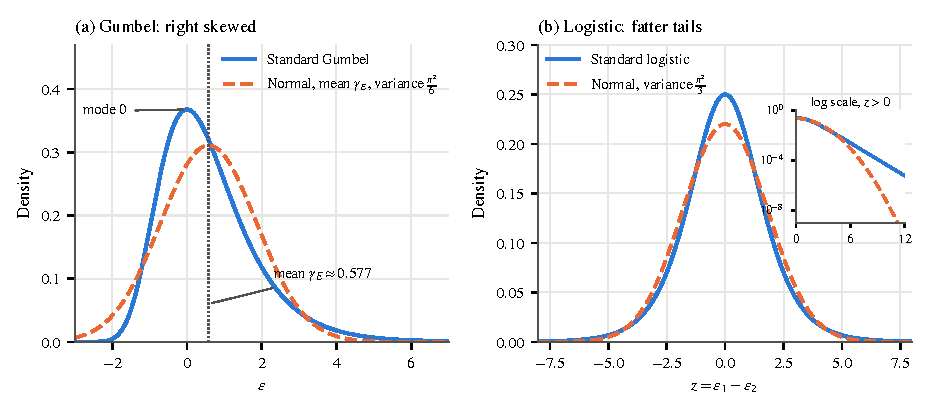
\includegraphics[width=\textwidth]{figures/ch06/gumbel_logistic.pdf}
\caption{Extreme value algebra. (a) The standard Gumbel density (mode $0$, mean $\gamma_E$) against a normal
density with the same mean and variance $\frac{\pi^2}{6}$. (b) The standard logistic density, the distribution of
the difference of two independent standard Gumbels, against a normal density with the same variance
$\frac{\pi^2}{3}$. The inset plots both densities on a log scale for $z > 0$.}
\label{fig:06-gumbel}
\end{figure}

\subsection{Logit choice probabilities}\label{sec:06-logitprob}

\begin{proposition}[Logit choice probabilities]\label{prop:06-logit}
Let $u_{ij} = V_{ij} + \sigma_\epsilon\epsilon_{ij}$ for $j = 0, 1, \dots, J$, with $\epsilon_{ij}$ independent and
identically distributed standard Gumbel and $\sigma_\epsilon > 0$. Then
\begin{equation}\label{eq:06-logit}
P_{ij} = \frac{\exp\left(\frac{V_{ij}}{\sigma_\epsilon}\right)}{\sum_{k=0}^J \exp\left(\frac{V_{ik}}{\sigma_\epsilon}\right)} .
\end{equation}
With $V_{i0} = 0$, $V_{ij} = \delta_j$ for $j \ge 1$ and $\sigma_\epsilon = 1$, the market share is
\begin{equation*}
s_j = \frac{e^{\delta_j}}{1 + \sum_{k=1}^J e^{\delta_k}} .
\end{equation*}
\end{proposition}

\begin{proof}[First proof (direct integration)]
Drop the index $i$ and fix $j$. Product $j$ is chosen when $V_j + \sigma_\epsilon\epsilon_j \ge V_k + \sigma_\epsilon\epsilon_k$
for every $k$, that is, when $\epsilon_k \le \epsilon_j + a_k$ with $a_k = \frac{V_j - V_k}{\sigma_\epsilon}$. Note that
$a_j = 0$. Condition on $\epsilon_j = e$. By independence,
\begin{align*}
P_j &= \int_{-\infty}^{\infty} f(e)\prod_{k\neq j}F(e + a_k)\,\dd e \\
&= \int_{-\infty}^{\infty} e^{-e}\exp\big(-e^{-e}\big)\prod_{k\neq j}\exp\big(-e^{-e}e^{-a_k}\big)\,\dd e \\
&= \int_{-\infty}^{\infty} e^{-e}\exp\Big(-e^{-e}\sum_{k=0}^J e^{-a_k}\Big)\,\dd e ,
\end{align*}
where the factor $\exp(-e^{-e})$ from the density supplies the term $k = j$, since $e^{-a_j} = 1$. Let
$A = \sum_{k=0}^J e^{-a_k} = \sum_{k=0}^J \exp\left(\frac{V_k - V_j}{\sigma_\epsilon}\right)$. Substitute $t = e^{-e}$,
with $\dd t = -e^{-e}\,\dd e$:
\begin{equation*}
P_j = \int_0^\infty e^{-At}\,\dd t = \frac{1}{A}
= \frac{\exp\left(\frac{V_j}{\sigma_\epsilon}\right)}{\sum_{k=0}^J \exp\left(\frac{V_k}{\sigma_\epsilon}\right)} . \qedhere
\end{equation*}
\end{proof}

\begin{proof}[Second proof (max-stability)]
Divide utilities by $\sigma_\epsilon$, which does not change choices (\cref{prop:06-normalization}). Let
$W_k = \frac{V_k}{\sigma_\epsilon}$. By \cref{lem:06-maxstable} applied to the alternatives other than $j$,
\begin{equation*}
\max_{k\neq j}(W_k + \epsilon_k) = L_{-j} + \epsilon^*, \qquad L_{-j} = \ln\sum_{k\neq j}e^{W_k},
\end{equation*}
where $\epsilon^*$ is standard Gumbel and independent of $\epsilon_j$. Product $j$ is chosen when
$W_j + \epsilon_j \ge L_{-j} + \epsilon^*$, that is, when $\epsilon^* - \epsilon_j \le W_j - L_{-j}$. By
\cref{lem:06-logistic},
\begin{equation*}
P_j = \Lambda(W_j - L_{-j}) = \frac{1}{1 + e^{L_{-j} - W_j}} = \frac{e^{W_j}}{e^{W_j} + \sum_{k\neq j}e^{W_k}} ,
\end{equation*}
which is \eqref{eq:06-logit}.
\end{proof}

\casehead{Income, constants and the normalization}
Terms common to all alternatives cancel from \eqref{eq:06-logit}. Consider
\begin{equation*}
u_{ij} = \bar u + \alpha(y_i - p_j) + x_j\beta + \xi_j + \sigma_\epsilon\epsilon_{ij}, \qquad
u_{i0} = \bar u + \alpha y_i + \sigma_\epsilon\epsilon_{i0},
\end{equation*}
with a common constant $\bar u$. The factor $\exp\big(\frac{\bar u + \alpha y_i}{\sigma_\epsilon}\big)$ appears in the
numerator and in every term of the denominator, so it cancels:
\begin{equation*}
P_{ij} = \frac{\exp\left(\frac{x_j\beta + \xi_j - \alpha p_j}{\sigma_\epsilon}\right)}
{1 + \sum_{k=1}^J\exp\left(\frac{x_k\beta + \xi_k - \alpha p_k}{\sigma_\epsilon}\right)} .
\end{equation*}
The probabilities depend on the parameters only through $\frac{\beta}{\sigma_\epsilon}$, $\frac{\alpha}{\sigma_\epsilon}$
and $\frac{\xi_j}{\sigma_\epsilon}$. Only one of the price coefficient and the scale of the shock can be normalized.
The usual choice sets $\sigma_\epsilon = 1$ and estimates $\alpha$, so that
$\delta_j = x_j\beta - \alpha p_j + \xi_j$ is measured in units of the shock. The alternative sets $\alpha = 1$
and estimates $\sigma_\epsilon$, so that utility is measured in dollars and $\sigma_\epsilon$ is the dollar scale of
the taste shocks. Writing $u_{ij} = (y_i - p_j) + \delta_j + \epsilon_{ij}$ with a standard Gumbel shock imposes
both normalizations at once. That specification assumes the standard deviation of the taste shock equals
$\frac{\pi}{\sqrt 6} \approx 1.28$ dollars, a restriction that the data cannot test once the price coefficient is fixed.

\casehead{The two limits of the scale}
Write \eqref{eq:06-logit} as
$P_j = \Big[\sum_k \exp\Big(\frac{V_k - V_j}{\sigma_\epsilon}\Big)\Big]^{-1}$. As $\sigma_\epsilon \to 0$, every term
with $V_k < V_j$ vanishes and every term with $V_k > V_j$ explodes. If $V_j$ is the unique maximum, then
$P_j \to 1$. If some $V_k$ exceeds $V_j$, then $P_j \to 0$. Choice becomes deterministic, and the consumer picks
$\arg\max_k V_k$. As $\sigma_\epsilon \to \infty$, every term tends to one, and $P_j \to \frac{1}{J+1}$. Choice
becomes uniform and ignores the attributes. The scale $\sigma_\epsilon$, or its inverse
$\mu_\epsilon = \frac{1}{\sigma_\epsilon}$, is the bridge to the ``modified BLP'' model of \citet{BerryPakes2007}.
BLP abbreviates the random coefficients logit of Berry, Levinsohn and Pakes \citep{BerryLevinsohnPakes1995}, the
subject of \cref{ch:blp}. The modified BLP model adds $\sigma_\epsilon\epsilon_{ij}$ to a pure characteristics model, and it approaches the pure
characteristics model as $\sigma_\epsilon \to 0$ (\cref{sec:06-epsilon}).

\begin{remark}[The logit as a model of tastes for products]\label{rem:06-tastesforproducts}
\citet[p.~1412]{McFadden1984} observes that the multinomial logit is a special case of a random coefficients
model in which only the coefficients of alternative-specific dummy variables are random. Write
\begin{equation*}
u_{ij} = V_{ij} + \sum_{k=0}^J \epsilon_{ik}\,d_{jk}, \qquad d_{jk} = \indic\{j = k\}.
\end{equation*}
The dummy $d_{jk}$ is a ``characteristic'' that only product $k$ possesses, and $\epsilon_{ik}$ is consumer $i$'s
random taste for it. \citet{BerryPakes2007} attribute this reading to \citet{CaplinNalebuff1991} and call such
models models with ``tastes for products''. Under this reading the dimension of the characteristic space grows
with the number of products. \Cref{sec:06-epsilon} shows that this growth drives the logit's implications for
markups and welfare as products are added.
\end{remark}

\subsection{Expected maximum utility and the log-sum formula}\label{sec:06-logsum}

\begin{proposition}[Log-sum formula]\label{prop:06-logsum}
Under the assumptions of \cref{prop:06-logit},
\begin{equation}\label{eq:06-logsum}
\E\Big[\max_k u_{ik}\Big] = \sigma_\epsilon\ln\sum_{k=0}^J\exp\left(\frac{V_{ik}}{\sigma_\epsilon}\right) + \sigma_\epsilon\gamma_E .
\end{equation}
Its gradient with respect to $(V_{i0}, \dots, V_{iJ})$ is the vector of logit probabilities
\eqref{eq:06-logit}. In addition, the distribution of the maximum utility does not depend on which alternative
attains it: for every $j$ and $x$,
\begin{equation}\label{eq:06-maxindep}
\Pr\Big(j \text{ chosen and } \max_k u_{ik} \le x\Big) = P_{ij}\,\Pr\Big(\max_k u_{ik} \le x\Big).
\end{equation}
\end{proposition}

\begin{proof}
Write $\max_k(V_k + \sigma_\epsilon\epsilon_k) = \sigma_\epsilon\max_k\big(\frac{V_k}{\sigma_\epsilon} + \epsilon_k\big)$. By
\cref{lem:06-maxstable}, $\max_k\big(\frac{V_k}{\sigma_\epsilon} + \epsilon_k\big)$ is Gumbel with location
$\ln\sum_k e^{\frac{V_k}{\sigma_\epsilon}}$ and scale one, so its mean is that location plus $\gamma_E$.
Multiplying by $\sigma_\epsilon$ gives \eqref{eq:06-logsum}. Differentiating,
\begin{equation*}
\frac{\partial}{\partial V_j}\left[\sigma_\epsilon\ln\sum_k e^{\frac{V_k}{\sigma_\epsilon}}\right]
= \sigma_\epsilon\cdot\frac{1}{\sigma_\epsilon}\,\frac{e^{\frac{V_j}{\sigma_\epsilon}}}{\sum_k e^{\frac{V_k}{\sigma_\epsilon}}} = P_j ,
\end{equation*}
as \cref{thm:06-wdz} requires.

For \eqref{eq:06-maxindep}, set $\sigma_\epsilon = 1$ without loss of generality. When $j$ is chosen, the maximum
equals $V_j + \epsilon_j$. Repeating the first proof of \cref{prop:06-logit} with the extra restriction
$V_j + e \le x$,
\begin{align*}
\Pr\Big(j \text{ chosen and } \max_k u_k \le x\Big)
&= \int_{-\infty}^{x - V_j} e^{-e}\exp\big(-Ae^{-e}\big)\,\dd e \\
&= \int_{e^{-(x - V_j)}}^{\infty} e^{-At}\,\dd t \\
&= \frac{1}{A}\exp\big(-Ae^{-(x - V_j)}\big),
\end{align*}
with $A = \sum_k e^{V_k - V_j}$. Since $\frac{1}{A} = P_j$ and $Ae^{V_j} = \sum_k e^{V_k}$, the last expression equals
$P_j\exp\big(-e^{-x}\sum_k e^{V_k}\big)$. By the proof of \cref{lem:06-maxstable} the second factor is
$\Pr(\max_k u_k \le x)$.
\end{proof}

Equation \eqref{eq:06-maxindep} says that the identity of the chosen alternative and the level of the maximum
utility are independent. Consumers who choose a product with low $V_j$ have, on average, a large
$\epsilon_j$ that exactly compensates. All buyers therefore enjoy the same expected utility, whatever they bought.
In the two-goods example of \cref{sec:06-twogoods}, the expected maximum utility is $\ln(1 + e^{0.5} + e) + \gamma_E \approx 2.26$.
A simulation with two million draws gives conditional means of $2.26$ for each of the three choices.

\casehead{Logit consumer surplus}
Combine \eqref{eq:06-logsum} with the welfare formula \eqref{eq:06-smallrosen}. Let
$u_{ij} = \alpha(y_i - p_j) + x_j\beta + \xi_j + \epsilon_{ij}$ for $j \ge 1$ and $u_{i0} = \alpha y_i + \epsilon_{i0}$,
with $\sigma_\epsilon = 1$ and $\delta_j = x_j\beta - \alpha p_j + \xi_j$. Then
$\E[\max_k u_{ik}] = \alpha y_i + \ln\big(1 + \sum_k e^{\delta_k}\big) + \gamma_E$, and dividing by the marginal utility
of income gives the expected consumer surplus
\begin{equation}\label{eq:06-logitcs}
CS_i = \frac{1}{\alpha}\ln\Big(1 + \sum_{k=1}^J e^{\delta_k}\Big) + C ,
\end{equation}
where $C = y_i + \frac{\gamma_E}{\alpha}$ is a constant that drops out of every comparison. For a change from a
choice set $\mathcal{J}^0$ with mean utilities $\delta^0$ to a choice set $\mathcal{J}^1$ with mean utilities $\delta^1$,
\begin{equation}\label{eq:06-logitdcs}
\Delta CS_i = \frac{1}{\alpha}\left[\ln\Big(1 + \sum_{k\in\mathcal{J}^1}e^{\delta^1_k}\Big)
- \ln\Big(1 + \sum_{k\in\mathcal{J}^0}e^{\delta^0_k}\Big)\right].
\end{equation}
Because $1 + \sum_k e^{\delta_k} = \frac{1}{s_0}$ in the logit, \eqref{eq:06-logitcs} can be written
$CS_i = -\frac{1}{\alpha}\ln s_0 + C$, and \eqref{eq:06-logitdcs} becomes
$\Delta CS_i = \frac{1}{\alpha}\ln\frac{s_0^0}{s_0^1}$. In the logit, the outside share and the price coefficient
alone determine the welfare change. In the two-goods example the rise in $\delta_1$ from $0.5$ to $1.3$
lowers $s_0$ from $0.186$ to $0.135$, a gain of $\ln\frac{0.186}{0.135} \approx 0.32$ utils, or
$\frac{0.32}{\alpha}$ dollars. Differentiating \eqref{eq:06-logitcs} with respect to $p_j$ gives
$-\frac{1}{\alpha}\cdot\frac{\alpha e^{\delta_j}}{1 + \sum_k e^{\delta_k}} = -s_j$, the logit version of the Roy
identity noted after \cref{cor:06-wdz}. The logit elasticities and the Berry inversion are in \cref{ch:logit},
and the welfare value of new goods is in \cref{ch:newgoods}. \Cref{sec:06-epsilon} shows that
\eqref{eq:06-logitdcs} assigns positive value to every added product, including an exact copy of an existing one.

\subsection{Luce's axiom, IIA and the generalized extreme value family}\label{sec:06-gev}

\casehead{The choice axiom and IIA}
\citet{Luce1959} proposed an axiom for probabilistic choice. Let $P(j \mid C)$ be the probability of choosing
$j$ from a set $C$. The \emph{choice axiom} requires $P(j \mid C) = P(j \mid A)\,P(A \mid C)$ for every subset
$A \subseteq C$ that contains $j$, where $P(A \mid C) = \sum_{k\in A}P(k \mid C)$. When all probabilities are
positive, the axiom implies that there are scale values $w_k > 0$ with
$P(j \mid C) = \frac{w_j}{\sum_{k \in C} w_k}$. The logit is the case $w_k = e^{V_k}$. The axiom is
equivalent to the \emph{independence of irrelevant alternatives} (IIA): the odds of choosing $j$ over $k$ do not
depend on the other alternatives. In the logit,
\begin{equation}\label{eq:06-iia}
\frac{P_j}{P_k} = \exp\left(\frac{V_j - V_k}{\sigma_\epsilon}\right) ,
\end{equation}
which depends only on $j$ and $k$. \citet[eq.~3.17, p.~1413]{McFadden1984} states the property for a model in
which $V_j = x_j\theta$ depends only on the attributes of $j$: $\ln\frac{P_j}{P_k} = (x_j - x_k)\theta$, independent
of the attributes of every other alternative.

IIA has three consequences. First, the probabilities for a smaller or larger choice set follow from
\eqref{eq:06-logit} by deleting or adding terms in the denominator. A model estimated on existing alternatives
can then forecast the demand for a new one, provided the new alternative brings no new parameters
\citep[p.~1414]{McFadden1984}. Second, the cross-elasticity of the probability of $j$ with respect to an attribute
of $k$ is the same for every $j \neq k$ (p.~1414). A rise in the price of $k$ sends its customers to the other
alternatives in proportion to their shares, as the two-goods example showed. Third, ranked data can be used.
The probability of a complete ranking is the product of logit probabilities of choosing the best alternative
from successively smaller sets \citep{Marschak1960}. \citet[p.~1414]{McFadden1984} calls IIA ``theoretically
implausible in many applications'', while noting that the logit often fits and predicts well in practice.

\begin{remark}[Why Gumbel]\label{rem:06-yellott}
Is the Gumbel distribution the only way to obtain Luce's axiom from random utility? \citet{Yellott1977} studies
random utility models with independent and identically distributed errors from a location family. He shows
that in this class the choice axiom holds for all choice sets of at least three alternatives only if the errors
are Gumbel. We
state the result without proof. It explains why the logit and the independent Gumbel model are the same
object.
\end{remark}

\begin{remark}[Universal logit]\label{rem:06-universal}
IIA comes from restricting $V_j$ to depend on the attributes of $j$ alone. The logistic functional form does
not imply it by itself. Suppose instead that $V_j = z_j(x)\theta$ may depend on the attributes $x$ of all
alternatives. Then the logit form
\begin{equation*}
P_j = \frac{e^{z_j(x)\theta}}{\sum_k e^{z_k(x)\theta}}
\end{equation*}
can approximate any continuous positive response probability model on a compact set, to any desired accuracy
\citep[eq.~3.18, pp.~1414--1415]{McFadden1984}. This \emph{universal logit} can describe any pattern of
cross-elasticities. The approximation may be computationally impractical, and it makes consistency with
utility maximization hard to impose or verify. Its main use is to suggest specification tests (p.~1415).
\end{remark}

The most common test of IIA uses the property that the logit parameters are the same on any subset of the
choice set. Let $\hat\beta_C$ and $\hat V_C$ be the estimates and their estimated covariance matrix from the full
choice set $C$, and $\hat\beta_D$ and $\hat V_D$ those from a subset $D$. Under IIA both estimators are consistent
and the full-set estimator is efficient, so
\begin{equation}\label{eq:06-hmtest}
S = (\hat\beta_D - \hat\beta_C)^\T(\hat V_D - \hat V_C)^{-1}(\hat\beta_D - \hat\beta_C)
\end{equation}
is asymptotically chi-squared with degrees of freedom equal to the rank of $\hat V_D - \hat V_C$
\citep[eq.~3.23, pp.~1417--1418]{McFadden1984}. \citet{HausmanMcFadden1984} analyze the test. McFadden warns
that it is an omnibus test and that it has little power unless the departures from the logit are substantial.
\Cref{ch:logit} applies it.

\begin{remark}[Aggregating alternatives]\label{rem:06-aggregation}
The logit form survives aggregation of alternatives into types \citep[eqs.~3.19--3.20, p.~1415]{McFadden1984}.
Suppose type $g$ contains $M_g$ elemental alternatives with attributes $x_{gj}$ and mean attributes
$\bar x_g$. The probability of choosing some alternative of type $g$ is
\begin{align*}
\sum_{j \in g}P_{gj} &= \frac{\sum_{j \in g}e^{x_{gj}\theta}}{\sum_h\sum_{l \in h}e^{x_{hl}\theta}}, \qquad
\sum_{j\in g}e^{x_{gj}\theta} = \exp\big(\bar x_g\theta + \ln M_g + \omega_g\big),
\end{align*}
where $\omega_g = \ln\Big[\frac{1}{M_g}\sum_{j\in g}e^{(x_{gj} - \bar x_g)\theta}\Big]$ corrects for heterogeneity
within the type and is zero when the alternatives in $g$ are identical. Choice among types is therefore a logit
with utility $\bar x_g\theta + \ln M_g + \omega_g$. The term $\ln M_g$ shows how the logit counts products. Doubling
the number of alternatives of a type, with the new ones identical to the old, adds $\ln 2$ to the utility of
the type. This is the tastes-for-products reading of \cref{rem:06-tastesforproducts} at
work.
\end{remark}

\begin{remark}[Sampling alternatives]\label{rem:06-sampling}
IIA has a practical use when the choice set is large, as when households choose among thousands of houses. The
denominator of each logit probability then sums over every alternative. \citet[sec.~3.6, pp.~1416--1417]{McFadden1984}
shows that the logit can be estimated from a sampled subset of alternatives for each consumer. Let $C$ be the full
choice set, and let consumer $i$ choose $j_i \in C$. The researcher draws a subset $\mathcal{D}_i \subseteq C$ that
contains $j_i$, under a known protocol that selects $\mathcal{D}$ with probability $r(\mathcal{D} \mid j_i, x_i)$. We
write $r$ for McFadden's $\pi$, which this book reserves for profit. The protocol must have the \emph{positive
conditioning property}: $r(\mathcal{D}_i \mid k, x_i) > 0$ for every $k \in \mathcal{D}_i$. Had any member of
$\mathcal{D}_i$ been chosen, the protocol could have produced the same subset.

The probability that consumer $i$ chose $k$, given the sampled subset, follows from Bayes' rule:
\begin{equation*}
\Pr(j_i = k \mid \mathcal{D}_i, x_i)
= \frac{P_k(x_i, \theta)\, r(\mathcal{D}_i \mid k, x_i)}{\sum_{l \in \mathcal{D}_i} P_l(x_i, \theta)\, r(\mathcal{D}_i \mid l, x_i)} .
\end{equation*}
The sum runs over $\mathcal{D}_i$ only, because the protocol never produces a subset that excludes the chosen
alternative. We substitute the logit $P_k(x_i, \theta) = \frac{e^{x_{ik}\theta}}{\sum_{m \in C}e^{x_{im}\theta}}$. The
full-set denominator appears in every term and cancels, which leaves
\begin{equation}\label{eq:06-sampled-logit}
\Pr(j_i = k \mid \mathcal{D}_i, x_i)
= \frac{\exp\big(x_{ik}\theta + \ln r(\mathcal{D}_i \mid k, x_i)\big)}{\sum_{l \in \mathcal{D}_i}\exp\big(x_{il}\theta + \ln r(\mathcal{D}_i \mid l, x_i)\big)} .
\end{equation}
This is a logit on $\mathcal{D}_i$ with $\ln r(\mathcal{D}_i \mid k, x_i)$ added to each utility. Positive conditioning
keeps every logarithm finite. The average of $\ln\Pr(j_i \mid \mathcal{D}_i, x_i)$ over consumers is McFadden's modified
log-likelihood (his eq.~3.22). Under positive conditioning and a standard identification condition, its maximizer is
consistent for $\theta$. It is a conditional likelihood, so the inverse of its information matrix estimates the
covariance matrix as usual (p.~1417).

The correction cancels when $r(\mathcal{D}_i \mid k, x_i)$ is the same for every $k \in \mathcal{D}_i$, the
\emph{uniform conditioning property}. McFadden's example draws the chosen alternative and one other alternative at
random (his eq.~3.21):
\begin{equation*}
r(\mathcal{D} \mid j_i, x_i) = \begin{cases} \frac{1}{|C| - 1} & \text{if } \mathcal{D} = \{j_i, k\} \text{ with } k \neq j_i,\\
0 & \text{otherwise,}\end{cases}
\end{equation*}
where $|C|$ is the number of alternatives. Either member of $\mathcal{D}_i$, had it been chosen, would have produced
$\mathcal{D}_i$ with the same probability. The logit can then be estimated from binary choices between the chosen
alternative and one random rival. The argument needs IIA. The full-set denominator cancels only because the ratio
$\frac{P_k}{P_l}$ does not depend on the alternatives outside $\mathcal{D}_i$.
\end{remark}

\casehead{Generalized extreme value models}
\citet{McFadden1978} found a class of joint distributions for the shocks that keeps closed forms while
relaxing IIA. Models in this class are called \emph{generalized extreme value} (GEV) models.

\begin{theorem}[Generalized extreme value models]\label{thm:06-gev}
Let $H : \R^{J+1}_+ \to \R_+$ satisfy three conditions.
\begin{enumerate}[label=(G\arabic*)]
  \item $H$ is homogeneous of degree one: $H(\lambda y) = \lambda H(y)$ for $\lambda > 0$.
  \item $H(y) \to \infty$ as $y_j \to \infty$, for any $j$.
  \item For any $r$ distinct indices $j_1, \dots, j_r$, the mixed partial derivative
  $\frac{\partial^r H}{\partial y_{j_1}\cdots\partial y_{j_r}}$ is nonnegative if $r$ is odd and nonpositive if $r$
  is even.
\end{enumerate}
Then the following hold.
\begin{enumerate}[label=(\alph*)]
  \item $F(\epsilon_0, \dots, \epsilon_J) = \exp\big(-H(e^{-\epsilon_0}, \dots, e^{-\epsilon_J})\big)$ is the CDF of a
  multivariate extreme value distribution whose marginals are Gumbel.
  \item In the ARUM $u_j = V_j + \epsilon_j$ with $\epsilon$ distributed as in (a), the choice probabilities are
  \begin{equation}\label{eq:06-gevprob}
  P_j = \frac{y_j H_j(y)}{H(y)} = \frac{\partial\ln H(e^{V_0}, \dots, e^{V_J})}{\partial V_j},
  \qquad y = (e^{V_0}, \dots, e^{V_J}),
  \end{equation}
  where $H_j$ is the partial derivative of $H$ with respect to its $j$-th argument.
  \item The social surplus function is $G(V) = \ln H(e^{V_0}, \dots, e^{V_J}) + \gamma_E$.
\end{enumerate}
\end{theorem}

\begin{proof}
Part (a) is the theorem of \citet{McFadden1978}, restated by \citet[eqs.~3.29--3.31, p.~1421]{McFadden1984}.
We take it as given. Its marginals follow by sending the other arguments to infinity:
$F_j(\epsilon_j) = \exp\big(-e^{-\epsilon_j}H(e_j)\big)$, a Gumbel CDF with location $\ln H(e_j)$, where $e_j$ is the
$j$-th unit vector.

For (c), the maximum is at most $x$ if and only if $\epsilon_k \le x - V_k$ for every $k$. Using (a) and then
homogeneity with $\lambda = e^{-x}$,
\begin{equation*}
\Pr\Big(\max_k(V_k + \epsilon_k) \le x\Big) = \exp\Big(-H\big(e^{V_0 - x}, \dots, e^{V_J - x}\big)\Big)
= \exp\Big(-e^{-\left(x - \ln H(y)\right)}\Big).
\end{equation*}
The maximum is Gumbel with location $\ln H(y)$, so its mean is $\ln H(y) + \gamma_E$.

For (b), the density of the event that $j$ is chosen with $\epsilon_j = e$ is $\frac{\partial F}{\partial\epsilon_j}$
evaluated at $\epsilon_k = e + V_j - V_k$ for all $k$. Differentiating $F$,
\begin{equation*}
\frac{\partial F}{\partial \epsilon_j}(\epsilon) = F(\epsilon)\,H_j(e^{-\epsilon_0}, \dots, e^{-\epsilon_J})\,e^{-\epsilon_j}.
\end{equation*}
At the evaluation point, $e^{-\epsilon_k} = \lambda y_k$ with $\lambda = e^{-e - V_j} = \frac{e^{-e}}{y_j}$. Homogeneity of
degree one implies $H(\lambda y) = \lambda H(y)$, and its derivative $H_j$ is homogeneous of degree zero, so
$H_j(\lambda y) = H_j(y)$. Hence
\begin{align*}
P_j &= \int_{-\infty}^{\infty}\exp\Big(-\frac{e^{-e}}{y_j}H(y)\Big)H_j(y)\,e^{-e}\,\dd e \\
&= H_j(y)\int_0^\infty\exp\Big(-t\,\frac{H(y)}{y_j}\Big)\,\dd t
= \frac{y_jH_j(y)}{H(y)},
\end{align*}
where the second line substitutes $t = e^{-e}$. Finally,
$\frac{\partial\ln H(e^{V})}{\partial V_j} = \frac{H_j(y)\,e^{V_j}}{H(y)}$, which is the same expression. It equals the
derivative of $G$ in (c), as \cref{thm:06-wdz} requires.
\end{proof}

The logit is the generating function $H(y) = \sum_j y_j$. It satisfies (G1) and (G2), its first derivatives
equal one, and its higher mixed derivatives vanish. Then $F(\epsilon) = \prod_j\exp(-e^{-\epsilon_j})$, the shocks
are independent, and \eqref{eq:06-gevprob} gives $P_j = \frac{y_j}{\sum_k y_k}$. McFadden's version,
$H(y) = \big(\sum_j y_j^{\frac{1}{\lambda}}\big)^{\lambda}$ with $0 < \lambda \le 1$, gives the logit with scale $\lambda$
\citep[eq.~3.32, p.~1421]{McFadden1984}.

The nested logit is the leading member of the family that relaxes IIA. Partition the inside products into nests
$g = 1, \dots, G$, and place the outside good in its own nest. With nesting parameter $\sigma \in [0, 1)$, let
\begin{equation}\label{eq:06-nestedH}
H(y) = y_0 + \sum_{g=1}^G\Big(\sum_{j\in g}y_j^{\frac{1}{1-\sigma}}\Big)^{1-\sigma}.
\end{equation}
Write $D_g = \sum_{k\in g}y_k^{\frac{1}{1-\sigma}}$. For $j$ in nest $g$, the derivative is
$H_j = D_g^{-\sigma}\,y_j^{\frac{\sigma}{1-\sigma}}$, so $y_jH_j = D_g^{-\sigma}y_j^{\frac{1}{1-\sigma}}$ and
\begin{equation*}
P_j = \frac{y_j^{\frac{1}{1-\sigma}}}{D_g}\cdot\frac{D_g^{1-\sigma}}{y_0 + \sum_{h=1}^G D_h^{1-\sigma}} .
\end{equation*}
The first factor is the probability of choosing $j$ within its nest, and the second is the probability of
choosing nest $g$. With $\sigma = 0$ the model is the logit. As $\sigma$ approaches one, the products within a
nest become close substitutes. \citet[sec.~3.10, pp.~1422--1425]{McFadden1984} develops the general
hierarchical version, the nested multinomial logit, with an ``independence'' parameter at each node, here
$1 - \sigma$. He notes that estimates of these parameters outside the unit interval indicate a misspecified tree
(pp.~1425--1426), and that the likelihood is not concave in all parameters (p.~1426). \Cref{ch:logit} develops
the nested logit, its elasticities and its estimation.

\subsection{The multinomial probit}\label{sec:06-probit}

The \emph{multinomial probit} assumes jointly normal shocks, $\epsilon_i \sim N(0, \Sigma_\epsilon)$, with a
$(J+1)\times(J+1)$ covariance matrix $\Sigma_\epsilon$. Product $j$ is chosen when
$\epsilon_{ik} - \epsilon_{ij} \le V_{ij} - V_{ik}$ for every $k \neq j$. The vector of these $J$ differences is
normal with covariance matrix $B_j\Sigma_\epsilon B_j^\T$, where $B_j$ is the $J\times(J+1)$ matrix that
subtracts $\epsilon_{ij}$ from the other shocks. The choice probability is a $J$-dimensional normal orthant
probability, which has no closed form \citep[sec.~3.8]{McFadden1984}. A version with an economic
interpretation sets $u_{ij} = x_{ij}a_i$ with normally distributed taste weights $a_i \sim N(\beta, \Omega_a)$, so
that utilities have covariance $x_i\Omega_a x_i^\T$ across alternatives (p.~1418).

The probit has the flexibility that the logit lacks. With correlated shocks it does not have IIA, and it
permits very general patterns of cross-elasticities (p.~1418). The cost is computation. McFadden reports that
probabilities with up to three alternatives cost about as much to compute as logit probabilities (p.~1418).
With five or more alternatives and an unrestricted covariance matrix, they were usually too costly for iterative
estimation at the time. The probit log-likelihood is also not known to be concave (p.~1419). One remedy restricts the
covariance with a factor structure,
\begin{equation*}
\epsilon_{ij} = \zeta_{ij} + \sum_{l=1}^{L}\gamma_{jl}v_{il},
\end{equation*}
with independent normal $\zeta_{ij}$ and $v_{il}$ \citep[eq.~3.25, p.~1419]{McFadden1984}. The loading $\gamma_{jl}$ can
be read as the level in alternative $j$ of an unobserved characteristic $l$, and $v_{il}$ as the consumer's random
taste for it. This is a random coefficients model on unobserved characteristics. Simulation methods developed
since then make probit models with many alternatives feasible \citep{Train2009}.

The independent probit, with $\Sigma_\epsilon$ the identity matrix, has essentially the same restrictions on
substitution as the logit, and \citet[p.~1420]{McFadden1984} sees little reason to prefer one over the other.
The lesson matters for the rest of the book. The logit's substitution problems come from shocks that are
independent across products, which leave products with no notion of similarity. The shape of the Gumbel
distribution plays little role. Fixing the problems requires correlation in tastes across similar products. Nesting supplies it within
groups (\cref{ch:logit}), and random coefficients on characteristics supply it along each characteristic
(\cref{ch:blp}).

\subsection{Choosing a functional form}\label{sec:06-forms}

\citet[sec.~3.3]{McFadden1984} judges functional forms by computational practicality and by flexibility in
representing similarity across alternatives. He groups the concrete forms into three families. Logit models
descend from \citet{Luce1959}. Probit models descend from \citet{Thurstone1927}. Elimination models, in which
alternatives are screened out until one remains, descend from \citet{Tversky1972}. His verdict (p.~1410) is that
the multinomial logit scores well on simplicity and computation but poorly on flexibility. The multinomial
probit is simple and flexible but scores poorly on computation. The nested logit and the factor-structure probit
try to achieve both. He adds that functional forms allowing similar substitution patterns tend to fit existing
data comparably. This observation anticipates the strategy of modern empirical work. The choice of a model is
mainly a choice of substitution patterns, and the distribution of the idiosyncratic shock matters mostly through
its implications for computation and welfare.

\begin{remark}[A representative-consumer foundation]\label{rem:06-representative}
Logit demand also arises from a single representative consumer \citep{AndersonDePalmaThisse1988,AndersonDePalmaThisse1992}.
Suppose the consumer allocates one unit of consumption across the alternatives $j = 0, 1, \dots, J$ to maximize
\begin{equation*}
\sum_{j=0}^J \delta_j q_j - \sum_{j=0}^J q_j\ln q_j \qquad \text{subject to} \qquad \sum_{j=0}^J q_j = 1,
\end{equation*}
with $\delta_0 = 0$. The entropy term rewards spreading consumption across products. The first-order conditions
$\delta_j - \ln q_j - 1 - \lambda = 0$, with multiplier $\lambda$, give $q_j \propto e^{\delta_j}$, and the constraint
yields $q_j = \frac{e^{\delta_j}}{1 + \sum_{k\ge 1}e^{\delta_k}}$, the logit shares. A weight $\sigma_\epsilon$ on the entropy
term produces the logit with scale $\sigma_\epsilon$. The two foundations, a population of consumers with Gumbel
shocks and a representative consumer with a taste for variety, give the same aggregate demand.
\Cref{ch:diffprod} gives the full derivation and shows that the constant elasticity of substitution (CES) demand system is a logit in log prices.
\end{remark}

\section{Models of product differentiation as random utility models}\label{sec:06-models}

The random utility model of \cref{sec:06-rum} is a general language for demand. A model of product
differentiation fills in two objects of that language. The first is the utility function
$U(x_j, p_j, \xi_j, \nu_i; \theta)$. The second is the distribution $F$ of the consumer tastes $\nu_i$. The
classical models of the theory literature (address models, ideal-point models, vertical models) and the
logit-type models of empirical work differ only in these two choices. This section places them in one
framework. The comparison matters because each specification fixes, before any data are used, which
products compete with which. Those restrictions drive every counterfactual the model produces.
\Cref{tab:06-taxonomy} at the end of the section collects the comparison.

\subsection{Horizontal and vertical differentiation}\label{sec:06-horvert}

Products are \emph{differentiated} when consumers do not regard them as perfect substitutes. Two polar
forms of differentiation organize the theory. They differ in whether consumers agree on how to rank the
products when prices are equal.

\begin{definition}[Vertical and horizontal differentiation]\label{def:06-vertical}
Let a consumer of type $\nu$ obtain utility $U(x_j, p, \nu)$ from product $j$ sold at price $p$. The
products are \emph{vertically differentiated} if at any common price every consumer ranks them in the
same order. Formally, for all products $j$ and $k$, all prices $p$, and all types $\nu$ and $\nu'$,
\begin{equation*}
  U(x_j, p, \nu) > U(x_k, p, \nu) \iff U(x_j, p, \nu') > U(x_k, p, \nu').
\end{equation*}
The products are \emph{horizontally differentiated} if at some common price two types rank some pair of
products differently.
\end{definition}

Under vertical differentiation a scalar index summarizes the common ranking. We call it \emph{quality}
and write it $\delta_j$. Consumers agree that higher quality is better. They disagree only about how much
extra money the extra quality is worth. Under horizontal differentiation no such index exists. At the same
price some consumers prefer a sweetened breakfast cereal and others a plain one, and neither group is
mistaken. Most markets mix the two forms. Every buyer prefers a luxury sedan to an economy sedan at the
same price, while buyers disagree about a sedan and a pickup truck.

The models below share a property that makes their demand systems tractable when tastes are
one-dimensional.

\begin{definition}[Single crossing]\label{def:06-singlecrossing}
Let the type $\nu$ be a scalar. Utility has the \emph{single-crossing property} if, for every pair of
products $j \ne k$ and all prices, the difference $U(x_j, p_j, \nu) - U(x_k, p_k, \nu)$ changes sign at
most once as $\nu$ increases. A sufficient condition is that the difference be strictly monotone in $\nu$.
\end{definition}

Under single crossing the utilities of two products, viewed as functions of the type, cross at most once.
The types that prefer $j$ to $k$ then form a half-line. The types that choose $j$ from the whole menu
form an interval, the intersection of such half-lines. Market shares become differences of the CDF $F$
evaluated at interval end points. Both the Hotelling model with quadratic transport costs and the
vertical model have this property. It is the reason their demand systems have closed forms, and the
reason each product competes only with its immediate neighbors.

\subsection{Address models: Hotelling and Salop}\label{sec:06-hotelling}

In an \emph{address model} each product has a location $x_j$ in a space of characteristics, and each
consumer has an ideal location in the same space. A consumer who buys a product away from her ideal
suffers a disutility that rises with the distance. \citet{Hotelling1929} introduced the idea with
consumers spread along a line. In random utility form, with quadratic distance costs,
\begin{equation}\label{eq:06-hotelling-u}
  u_{ij} = \bar u + (y_i - p_j) - \tau\, d(x_j, \nu_i)^2,
\end{equation}
where $\bar u$ is a utility constant common to all consumers, $y_i$ is income, $\nu_i$ is the consumer's
ideal location, and $d$ is distance. The coefficient $\tau > 0$ is the \emph{transport cost}. We reserve
$\theta$ for the generic parameter vector of \cref{sec:06-rum}, so the transport cost is always $\tau$.
The taste $\nu_i$ is now a location, and its distribution $F$ plays the role that the error distribution
plays in an additive random utility model. Products are horizontally differentiated. At equal prices
each consumer ranks products by distance, and consumers at different locations disagree.

\begin{example}[Hotelling duopoly with quadratic transport costs]\label{ex:06-hotelling}
Two firms sit at the ends of the unit interval, $x_1 = 0$ and $x_2 = 1$, and produce at common marginal
cost $c$. A mass $M$ of consumers is uniform on $[0,1]$, so $F(\nu) = \nu$. A consumer who buys nothing
obtains $y_i$. We assume $\bar u$ is large enough that every consumer buys one unit (full coverage).
Income and $\bar u$ then enter both inside utilities and cancel from the comparison.

The first step finds the indifferent consumer. A consumer at $\nu$ prefers firm 1 if
$-p_1 - \tau\nu^2 > -p_2 - \tau(1-\nu)^2$. The indifferent type $\nu^*$ solves
\begin{align*}
  p_1 + \tau(\nu^*)^2 &= p_2 + \tau(1-\nu^*)^2,\\
  \tau\big[(\nu^*)^2 - (1-\nu^*)^2\big] &= p_2 - p_1,\\
  \tau(2\nu^* - 1) &= p_2 - p_1,
\end{align*}
so that
\begin{equation}\label{eq:06-hotelling-cut}
  \nu^* = \frac{1}{2} + \frac{p_2 - p_1}{2\tau}.
\end{equation}
The utility difference $u_{i1} - u_{i2} = p_2 - p_1 + \tau(1 - 2\nu_i)$ falls in $\nu_i$ (single
crossing), so every consumer to the left of $\nu^*$ buys from firm 1.

The second step writes demand. Firm 1 sells $q_1 = M F(\nu^*) = M\nu^*$ and firm 2 sells
$q_2 = M(1 - \nu^*)$. These formulas hold when $0 < \nu^* < 1$, that is, when $|p_2 - p_1| < \tau$.
Demand is linear in prices, with $\frac{\partial q_1}{\partial p_1} = -\frac{M}{2\tau}$.

The third step finds best responses. Firm 1 maximizes $\pi_1 = (p_1 - c)M\nu^*(p_1, p_2)$, a concave
quadratic in $p_1$. Its first-order condition is
\begin{equation*}
  M\Big[\nu^* - \frac{p_1 - c}{2\tau}\Big] = 0.
\end{equation*}
Substituting \eqref{eq:06-hotelling-cut} gives $\frac{1}{2} + \frac{p_2 - p_1}{2\tau} = \frac{p_1 - c}{2\tau}$.
Multiplying by $2\tau$ and collecting terms gives the best response
\begin{equation*}
  p_1 = \frac{p_2 + c + \tau}{2}.
\end{equation*}

The fourth step imposes symmetry. With $p_1 = p_2 = p$, the best response becomes $p = \frac{p + c + \tau}{2}$,
so
\begin{equation}\label{eq:06-hotelling-eq}
  p_1 = p_2 = c + \tau, \qquad \nu^* = \frac{1}{2}, \qquad \pi_1 = \pi_2 = \frac{M\tau}{2}.
\end{equation}
The markup equals the transport cost. As $\tau \to 0$ the two products become perfect substitutes and
the price falls to marginal cost, the Bertrand outcome of \cref{ch:theory}. Full coverage holds in this
equilibrium when the consumer at $\nu = \frac{1}{2}$ prefers buying, $\bar u - c - \tau - \frac{\tau}{4}
\ge 0$, that is, $\bar u \ge c + \frac{5\tau}{4}$. The equilibrium is the case $x_1 = 0$, $x_2 = 1$ of
\cref{prop:04-hotelling}. Linear transport costs with the firms at the end points give the same indifferent
consumer and the same prices (\cref{sec:04-hotelling-linear}).
\end{example}

The quadratic form of the transport cost keeps demand continuous. With linear costs
$\tau\, d(x_j, \nu_i)$, demand jumps when one firm cuts its price far enough below its rival's to capture
the consumers at the rival's own location. \citet{DAspremontGabszewiczThisse1979} show that no pure-strategy
price equilibrium then exists when the two firms are located near the center of the line at distinct points
(\cref{prop:04-dgt}). With quadratic costs a price equilibrium exists for every pair of locations. In the two-stage game in which firms first choose locations and then prices, the firms move to
the two ends of the line, because distance softens price competition. \Cref{prop:04-hotelling} derives this
maximal differentiation in the location stage, and \cref{sec:04-hotelling-quad} shows that it exceeds the
efficient differentiation.

\citet{Salop1979} removed the end points of the line by placing consumers on a circle. Consider $N$ firms
spaced evenly on a circle of circumference one, each with marginal cost $c$. Transport cost is linear with
coefficient $\tau$. A mass $M$ of consumers is uniform on the circle, and every consumer buys. Take a firm that
charges $p$ while its two neighbors, each at distance $\frac{1}{N}$, charge $\bar p$. A consumer at distance $z$
from the firm, on the arc toward a neighbor, is indifferent when
\begin{equation*}
  p + \tau z = \bar p + \tau\Big(\frac{1}{N} - z\Big),
  \qquad\text{so}\qquad
  z = \frac{1}{2N} + \frac{\bar p - p}{2\tau}.
\end{equation*}
The firm serves consumers on both arcs, so its demand is
\begin{equation*}
  q = 2Mz = M\Big[\frac{1}{N} + \frac{\bar p - p}{\tau}\Big] \qquad\text{for } |\bar p - p| \le \frac{\tau}{N}.
\end{equation*}
Demand depends on the prices of the two neighbors and on no other price. By \cref{prop:04-salop}, the symmetric
equilibrium price is $p = c + \frac{\tau}{N}$, so the markup falls as products crowd the circle. With a fixed cost
of entry, free entry yields twice the efficient number of firms. Every consumer buys, so the markup is a
transfer, and the only distortion is in the number of firms. An entrant takes business from its neighbors,
while society gains only the saving in transport costs \citep[sec.~7.1.2]{Tirole1988}. Entry remains excessive
with quadratic transport costs (\cref{sec:04-salop}). Each firm in the Salop model competes only with its two
neighbors, a feature it shares with the vertical model below.

\subsection{The ideal-point model}\label{sec:06-idealpoint}

The address model extends to $K$ characteristics. In the \emph{ideal-point model}
\citep{AndersonDePalmaThisse1992} consumer $i$ has an ideal level $\nu_{ik}$ of each characteristic $k$,
and utility is
\begin{equation}\label{eq:06-idealpoint}
  u_{ij} = f(y_i, p_j) + \delta_j - \sum_{k=1}^K \alpha_k (x_{jk} - \nu_{ik})^2, \qquad \alpha_k > 0.
\end{equation}
Here $f(y_i, p_j)$ is the utility of the income left after the purchase, with $f_y > 0$, $f_p < 0$ and
$f_{py} \ge 0$ as in \cref{sec:06-normalization}. The term $\delta_j$ is a product effect common to all
consumers, and $\alpha_k$ is the weight of distance along dimension $k$. We write the distance term with
a minus sign and positive weights, so that utility falls with distance.\footnote{Some presentations
write the distance term with a plus sign. The weights must then be negative for distance to be costly.
We use the minus sign with positive weights.} The next result shows that
the ideal-point model is a special case of the pure characteristics model introduced below.

\begin{proposition}[Ideal points are random coefficients]\label{prop:06-idealpoint}
Under \eqref{eq:06-idealpoint},
\begin{equation}\label{eq:06-idealpoint-expanded}
  u_{ij} = f(y_i, p_j) + \Big[\delta_j - \sum_{k=1}^K \alpha_k x_{jk}^2\Big]
           + \sum_{k=1}^K 2\alpha_k\nu_{ik}\, x_{jk} - \sum_{k=1}^K \alpha_k\nu_{ik}^2 .
\end{equation}
Consequently, the following hold.
\begin{enumerate}[label=(\roman*)]
  \item Comparisons among inside products depend on the tastes only through the interactions
        $\nu_{ik}x_{jk}$. The model is a random coefficients model without an idiosyncratic shock. Its mean
        utility is $\delta_j - \sum_k \alpha_k x_{jk}^2$, and characteristic $x_{jk}$ carries the random
        coefficient $2\alpha_k\nu_{ik}$.
  \item The term $-\sum_k \alpha_k\nu_{ik}^2$ is the same for every inside product, so it cancels from
        every comparison among them. Relative to an outside good with utility $f(y_i, 0)$, it acts as a
        random coefficient on a characteristic that equals one for every inside product.
\end{enumerate}
\end{proposition}

\begin{proof}
Expand each square:
\begin{equation*}
  (x_{jk} - \nu_{ik})^2 = x_{jk}^2 - 2x_{jk}\nu_{ik} + \nu_{ik}^2 .
\end{equation*}
Multiply by $-\alpha_k$ and sum over $k$:
\begin{equation*}
  -\sum_k \alpha_k (x_{jk} - \nu_{ik})^2 = -\sum_k \alpha_k x_{jk}^2 + \sum_k 2\alpha_k\nu_{ik}x_{jk}
  - \sum_k \alpha_k\nu_{ik}^2 .
\end{equation*}
Substituting into \eqref{eq:06-idealpoint} gives \eqref{eq:06-idealpoint-expanded}. For two inside
products $j$ and $l$,
\begin{equation*}
  u_{ij} - u_{il} = f(y_i, p_j) - f(y_i, p_l) + \Big[\delta_j - \sum_k \alpha_k x_{jk}^2\Big]
  - \Big[\delta_l - \sum_k \alpha_k x_{lk}^2\Big] + \sum_k 2\alpha_k\nu_{ik}(x_{jk} - x_{lk}),
\end{equation*}
in which $\nu_{ik}^2$ no longer appears. This proves (i) and the first part of (ii). The difference
$u_{ij} - u_{i0}$ keeps the term $-\sum_k \alpha_k\nu_{ik}^2$, which is the product of a consumer-specific
coefficient and the constant one. This proves the rest of (ii).
\end{proof}

\citet[eq.~6]{BerryPakes2007} make the same point. They write the ideal-point model with a distance
between the consumer's location and the product's location. With Euclidean distance, they note, expanding
the squares leaves a mean utility that depends on characteristics. The individual term is then built from
interactions of consumer and product characteristics. The quadratic term
$-\alpha_k x_{jk}^2$ in mean utility is what distinguishes ideal points from linear random coefficients.
It makes the value of a characteristic peak at the consumer's ideal and decline beyond it. With linear
random coefficients and tastes $\nu_{ik}$ of both signs, consumers also disagree about the direction in
which a characteristic is good, which is another form of horizontal differentiation.

\subsection{Two families of empirical models}\label{sec:06-classes}

The empirical models of this book fall into two families. The first is the \emph{pure characteristics
model} \citep{BerryPakes2007}, in which consumers have tastes for characteristics and for nothing else:
\begin{equation}\label{eq:06-pc-class}
  u_{ij} = f(y_i, p_j) + \delta_j + \sum_{k=1}^K \sigma_k \nu_{ik} x_{jk}.
\end{equation}
Here $\nu_{ik}$ is a standardized taste for characteristic $k$ and $\sigma_k \ge 0$ its dispersion, the
$k$-th diagonal element of the matrix $\Sigma$ in the random coefficients notation of \cref{ch:blp}. The
model is also called the \emph{pure hedonic} model. By \cref{prop:06-idealpoint}, the ideal-point model
belongs to this family once its quadratic terms are counted among the characteristics and a constant
inside-good characteristic is added. The second family adds an idiosyncratic shock $\epsilon_{ij}$:
\begin{equation}\label{eq:06-blp-class}
  u_{ij} = f(y_i, p_j) + \delta_j + \sum_{k=1}^K \sigma_k \nu_{ik} x_{jk} + \epsilon_{ij},
\end{equation}
with $\epsilon_{ij}$ i.i.d.\ across products and consumers. With type-I extreme value shocks this is the
random coefficients logit model of \citet{BerryLevinsohnPakes1995}, the subject of \cref{ch:blp}. With
$\sigma_k = 0$ for all $k$ it is the logit model of \cref{sec:06-tiev}.

The function $f$ carries income effects. In the quasi-linear case $f(y_i, p_j) = \alpha(y_i - p_j)$ income
enters every alternative equally and cancels, and the price coefficient $\alpha$ is common to all
consumers. \citet{BerryLevinsohnPakes1995} use $f(y_i, p_j) = \alpha\ln(y_i - p_j)$, which makes richer
consumers less price sensitive ($f_{py} > 0$). The properties of $f$ are derived in
\cref{sec:06-normalization}.

The key difference between \eqref{eq:06-pc-class} and \eqref{eq:06-blp-class} is the shock
$\epsilon_{ij}$. With $\epsilon_{ij}$ in the model, the product space can never be exhausted. Each new
product arrives with a fresh draw of $\epsilon_{ij}$ for every consumer, which guarantees it a positive
share and some market power wherever it is placed. In the pure characteristics model a new product placed
next to an existing one is a near-perfect substitute for it. \Cref{sec:06-epsilon} develops the
consequences for markups and for the welfare value of new products. The vertical model, to which we now
turn, is the pure characteristics model with a single characteristic, quality, and a single random
coefficient, on price.

\subsection{The vertical model as a random utility model}\label{sec:06-vdef}

The \emph{vertical model} specifies
\begin{equation}\label{eq:06-vertical-u}
  u_{ij} = \delta_j - \nu_i p_j, \qquad \nu_i > 0,
\end{equation}
with outside good $u_{i0} = 0$. The products are vertically differentiated in the sense of
\cref{def:06-vertical}. At any common price $p$, $u_{ij} - u_{ik} = \delta_j - \delta_k$ for every consumer,
so all consumers rank products by $\delta_j$. Consumers differ only in their \emph{price sensitivity}
$\nu_i$, the utility cost of a dollar. A consumer with high $\nu_i$ dislikes paying and buys cheap,
low-quality products. A consumer with low $\nu_i$ pays a lot for quality. The cabins of an airline (first,
business, economy) fit this description. Every traveler prefers the front cabin at equal prices, and
travelers sort across cabins by willingness to pay. Storage or memory tiers of an otherwise identical device are a
second example.

Dividing \eqref{eq:06-vertical-u} by $\nu_i > 0$ gives an equivalent form. With $v_i = \frac{1}{\nu_i}$,
\begin{equation}\label{eq:06-vertical-v}
  \frac{u_{ij}}{\nu_i} = v_i\delta_j - p_j .
\end{equation}
Here $v_i$ is the consumer's willingness to pay for a unit of quality. A consumer-specific positive
rescaling of utility leaves choices unchanged (\cref{sec:06-normalization}), so the two forms imply the
same demand. The form \eqref{eq:06-vertical-v} is the one used by \citet{MussaRosen1978} and by
\citet{Bresnahan1987}, who attributes the demand system to \citet{PrescottVisscher1977}. In this form the
consumer buys the product with the lowest ``total price'' $p_j - v_i\delta_j$.

The vertical model has the single-crossing property. For two products with $p_k > p_j$,
\begin{equation}\label{eq:06-vertical-sc}
  u_{ij} - u_{ik} = (\delta_j - \delta_k) + \nu_i(p_k - p_j)
\end{equation}
is strictly increasing in $\nu_i$. The preference for the cheaper product rises with price sensitivity.
More generally, consider any model with a scalar type in which all consumers agree on the quality ranking.
It is vertical and single crossing whenever the marginal rate of substitution between quality and money
is monotone in the type. \citet{GabszewiczThisse1979} obtain such a model from income differences. In their specification
$u_{ij} = \delta_j(y_i - p_j)$, and a consumer with income $y$ prefers $j$ to $k$ (with $\delta_j > \delta_k$
and $p_j > p_k$) if and only if
\begin{equation*}
  \delta_j(y - p_j) > \delta_k(y - p_k)
  \iff y(\delta_j - \delta_k) > \delta_j p_j - \delta_k p_k
  \iff y > \frac{\delta_j p_j - \delta_k p_k}{\delta_j - \delta_k} .
\end{equation*}
Richer consumers buy higher quality, and the cutoffs now live in income space. \citet{ShakedSutton1982}
embed this demand system in a two-stage game. Firms first choose qualities and then compete in prices,
and in equilibrium they choose distinct qualities to relax price competition. \citet{MussaRosen1978}
study a monopolist that offers a menu of qualities to consumers with utility $v_i\delta - p$. The
monopolist screens consumers by quality and supplies every type except the highest a quality below the
efficient level. These theory results take the vertical structure as given. \Cref{sec:06-vertical}
develops its demand side for estimation.

\subsection{The logit as a model of differentiation}\label{sec:06-logitdiff}

The logit model $u_{ij} = \delta_j - \alpha p_j + \epsilon_{ij}$, with $\epsilon_{ij}$ i.i.d.\ type-I extreme
value (\cref{prop:06-logit}), is also a model of differentiation. Each product carries its own taste
dimension. \Cref{rem:06-tastesforproducts} reads the shock $\epsilon_{ij}$ as consumer $i$'s random taste for
a characteristic that only product $j$ possesses, the product's own dummy variable. Under this reading, which
\citet{BerryPakes2007} attribute to \citet{CaplinNalebuff1991}, the characteristic space of the logit has one
dimension per product. Adding a product adds a dimension, so every product owns a
neighborhood of taste space that no rival can enter. This is the formal content of the statement that
the product space is never exhausted.

The logit treats every pair of products as equally distant. Consumers who leave a product spread over the
others in proportion to their shares, the independence of irrelevant alternatives property examined in
\cref{sec:06-gev} and \cref{ch:logit}. \citet{AndersonDePalmaThisse1989} give the logit a deterministic address
representation, with no random utility shock. Their consumers have ideal points as in \eqref{eq:06-idealpoint}, with
utility linear in price and a common weight on every characteristic. With $J$ products and no outside good, each
demand rises strictly with every rival price, at every price vector, only if the products span at least $J-1$
dimensions \citep[Proposition~1]{AndersonDePalmaThisse1989}. We follow \citet{AndersonDePalmaThisse1989} and place
product $J$ at the origin and each product $j<J$ at the same distance along the axis of characteristic $j$. These
locations span exactly $J-1$ dimensions. We also give the products equal quality. Logit demand then arises from a
unique density of ideal points, which has a single peak at the point equidistant from all products
\citep[Propositions~2 and~4]{AndersonDePalmaThisse1989}. Other locations that span $J-1$ dimensions also give a
unique density, though a different one \citep[p.~26]{AndersonDePalmaThisse1989}.
The nested logit adds a taste common to the products of a group, and the random coefficients logit adds
tastes for characteristics. Both keep the product-specific shock. \Cref{tab:06-taxonomy} summarizes how
the models differ.

\begin{table}[htbp]
\centering
\caption{Discrete choice models of product differentiation compared}\label{tab:06-taxonomy}
\footnotesize
\renewcommand{\arraystretch}{1.3}
\begin{tabularx}{\textwidth}{@{}>{\raggedright\arraybackslash}p{3.0cm}>{\raggedright\arraybackslash}p{1.55cm}>{\raggedright\arraybackslash}X>{\raggedright\arraybackslash}p{1.1cm}>{\raggedright\arraybackslash}p{2.05cm}>{\raggedright\arraybackslash}p{2.0cm}@{}}
\toprule
Model and utility & Dimension of heterogeneity & Who substitutes with whom & Closed-form shares & Markups as products crowd the space & Surplus from an added clone \\
\midrule
Hotelling, Salop\newline $-p_j - \tau\, d(x_j,\nu_i)^2$ & 1 (location) & Neighbors on the line or circle & Yes & Fall to zero ($\frac{\tau}{N}$ in Salop) & Zero \\
Ideal point\newline $\delta_j - p_j$\newline $-\sum_k \alpha_k(x_{jk}-\nu_{ik})^2$ & $K$ (ideal points) & Products close in characteristic space & No & Fall to zero & Zero \\
Pure characteristics\newline $\delta_j - \alpha p_j + \sum_k \sigma_k\nu_{ik}x_{jk}$ & $K$ (tastes for characteristics) & Products close in characteristics and price & No & Fall to zero & Zero \\
Vertical\newline $\delta_j - \nu_i p_j$ & 1 (price sensitivity) & Price neighbors only & Yes & Fall to zero for neighbors owned by rivals & Zero \\
Logit\newline $\delta_j - \alpha p_j + \epsilon_{ij}$ & $J$ (one taste per product) & All products, in proportion to shares & Yes & Bounded below by $\frac{1}{\alpha}$ & Positive \\
Nested logit\newline $\delta_j - \alpha p_j + \zeta_{ig}$\newline $+\,(1-\sigma)\epsilon_{ij}$ & $J$ plus one per nest & Mostly within the nest, in proportion to shares & Yes & Bounded below by $\frac{1-\sigma}{\alpha}$ & Positive \\
Random coefficients logit\newline $\delta_j - \alpha p_j + \sum_k \sigma_k\nu_{ik}x_{jk}$\newline $+\,\epsilon_{ij}$ & $K$ plus $J$ & Mostly toward products with similar characteristics & No & Bounded away from zero & Positive \\
\bottomrule
\end{tabularx}
\par\smallskip
\begin{minipage}{\textwidth}
\footnotesize Notes: Utilities omit income, which cancels under quasi-linearity. $\tau$ is the transport cost,
$d$ a distance, $\nu_i$ the consumer's type, and $\sigma_k$ the dispersion of the taste for characteristic
$k$. In the nested logit, $\sigma \in [0,1)$ is the nesting parameter and $\zeta_{ig}$ is a taste for nest $g$
whose distribution makes $\zeta_{ig} + (1-\sigma)\epsilon_{ij}$ type-I extreme value. Markup bounds are for single-product
firms facing an outside good. ``Surplus from an added clone'' is the gain in expected consumer surplus,
at fixed prices, from adding an exact copy of an existing product. \Cref{sec:06-epsilon} derives the logit
entries, and \cref{ch:logit,ch:blp} treat the nested and random coefficients logit.
\end{minipage}
\end{table}

\section{The vertical model}\label{sec:06-vertical}

The vertical model is the simplest model in characteristic space that delivers closed-form demand, an
exact inversion from market shares to qualities, and a transparent supply side. It is the demand system of
the first structural test of conduct in a differentiated-products industry \citep{Bresnahan1987}, the
case study of \cref{sec:06-bresnahan}. It is also the building block from which \citet{BerryPakes2007}
compute shares in the pure characteristics model (\cref{sec:06-purechar}). This section develops the
model for a general taste distribution $F$, then specializes to exponential and uniform tastes. Every
derivation is carried out in the notation of \eqref{eq:06-vertical-u}.

\subsection{Setup and the ordering of products}\label{sec:06-vsetup}

\begin{assumption}[Vertical model]\label{ass:06-vertical}
\leavevmode
\begin{enumerate}[label=(\roman*)]
  \item A market has $M$ consumers and $J$ inside products. Consumer $i$ obtains $u_{ij} = \delta_j - \nu_i p_j$
        from product $j$, where $\delta_j$ is the product's quality and $p_j > 0$ its price.
  \item The outside good $j = 0$ has $\delta_0 = p_0 = 0$, so $u_{i0} = 0$.
  \item The price sensitivities $\nu_i$ are i.i.d.\ draws from a distribution with continuous and strictly
        increasing CDF $F$ on $(0,\infty)$ and density $f = F' > 0$. We set $F(x) = 0$ for $x \le 0$.
  \item Each consumer buys one unit of the product with the highest utility.
  \item Inside prices are distinct.
\end{enumerate}
\end{assumption}

Part (iii) makes ties a probability-zero event, so choices are well defined for almost every consumer. The
quality $\delta_j$ summarizes everything consumers value about product $j$, observed and unobserved. In
estimation we write $\delta_j = x_j\beta + \xi_j$. Part (v) is generic. If two products had the same price,
every consumer would buy the higher-quality one, and the other would sell nothing. The price sensitivity
is the only dimension of consumer heterogeneity. Consumers agree on how characteristics combine into
quality and disagree only on the marginal utility of money.

\begin{lemma}[Ordering]\label{lem:06-ordering}
Under \cref{ass:06-vertical}, if $p_j > p_k$ and product $j$ sells a positive quantity, then
$\delta_j > \delta_k$. Hence the products with positive sales, together with the outside good, can be
indexed so that
\begin{equation}\label{eq:06-ordering}
  0 = p_0 < p_1 < \dots < p_J \qquad\text{and}\qquad 0 = \delta_0 < \delta_1 < \dots < \delta_J .
\end{equation}
\end{lemma}

\begin{proof}
Suppose $p_j > p_k$ and $\delta_j \le \delta_k$. For every $\nu > 0$,
\begin{equation*}
  u_j(\nu) - u_k(\nu) = (\delta_j - \delta_k) - \nu(p_j - p_k) \le -\nu(p_j - p_k) < 0 .
\end{equation*}
Every consumer strictly prefers $k$ to $j$, so $j$ sells nothing. The contrapositive is the first claim.
Applying it with $k = 0$ shows that every product with positive sales has $\delta_j > 0$. Applying it to
every pair of products with positive sales orders their qualities as their prices.
\end{proof}

Among products that sell, price and quality rise together. A product that charges more than a rival and
offers less quality loses every consumer to that rival. We say it is \emph{dominated outright}. A subtler
form of domination is possible. A product can offer more quality than every cheaper product and still sell
nothing, because a combination of two rivals beats it for every consumer. The geometry of the
$(p, \delta)$ plane makes this precise.

\begin{proposition}[The quality-price frontier]\label{prop:06-frontier}
Let $\mathcal P = \{(p_0, \delta_0), (p_1, \delta_1), \dots, (p_J, \delta_J)\}$ be the points of the
$(p, \delta)$ plane occupied by the outside good and the $J$ products, with prices distinct but qualities
arbitrary. Under \cref{ass:06-vertical} the following hold.
\begin{enumerate}[label=(\roman*)]
  \item A consumer of type $\nu$ chooses product $j$ if and only if every other point of $\mathcal P$ lies
        strictly below the line through $(p_j, \delta_j)$ with slope $\nu$.
  \item Product $j \ge 1$ sells a positive quantity if and only if $(p_j, \delta_j)$ is a vertex of the
        \emph{quality-price frontier}. The frontier is the rising part of the upper boundary of the
        convex hull of $\mathcal P$.
  \item Equivalently, delete the products that sell nothing and index the rest by price. Then the slopes
        $\bar\nu_j = \frac{\delta_j - \delta_{j-1}}{p_j - p_{j-1}}$, $j = 1, \dots, J$, satisfy
        $\bar\nu_1 > \bar\nu_2 > \dots > \bar\nu_J > 0$.
\end{enumerate}
\end{proposition}

\begin{proof}
For (i), type $\nu$ chooses $j$ if and only if $\delta_j - \nu p_j > \delta_k - \nu p_k$ for all $k \ne j$.
Rearranging, this holds if and only if
\begin{equation*}
  \delta_k < \delta_j + \nu(p_k - p_j) \qquad \text{for all } k \ne j .
\end{equation*}
The right side is the height at $p_k$ of the line through $(p_j, \delta_j)$ with slope $\nu$.

For (ii), consider lines through $(p_j, \delta_j)$ that lie strictly above every other point of
$\mathcal P$. Such a line exists if and only if $(p_j, \delta_j)$ is a vertex of the upper boundary of the
convex hull of $\mathcal P$. Let $a_j$ be the slope of the hull edge to the left of that vertex. Let $b_j$ be
the slope of the edge to its right, with $b_j = -\infty$ at the right end of the hull. Concavity of the
upper boundary gives $a_j > b_j$. A line through the vertex lies strictly above all other points if and
only if its slope lies in the open interval $(b_j, a_j)$. By (i), the types that choose $j$ form the set
$(b_j, a_j) \cap (0, \infty)$. Because $F$ has a positive density on $(0,\infty)$, this set has positive
probability if and only if $a_j > 0$. In words, the vertex must lie on the rising part of the hull. The
share is then $F(a_j) - F(\max\{b_j, 0\})$. A point that lies on a hull edge without being a
vertex is chosen at most by the single type whose slope equals that edge's slope, a probability-zero
event.

For (iii), the products that sell are the vertices of the rising part of the hull. Indexed by price, the
edges between consecutive vertices have strictly decreasing slopes, because the upper boundary is
strictly concave at each vertex. The last slope is positive because the hull rises up to the
highest-quality product. Conversely, suppose the slopes of the chain through the remaining points are
positive and strictly decreasing. Then the chain is strictly concave and rising, so every point on it is a
vertex of the frontier.
\end{proof}

\Cref{fig:06-frontier} draws the frontier. The slopes of its edges are the \emph{cutoffs} studied in
\cref{sec:06-vcutoffs}. A product strictly below the frontier sells nothing. We say it is
\emph{dominated out of the market}. Two cases arise in the figure. Product $a$ is dominated outright by
product 1, which is cheaper and better. Product $b$ has more quality than every cheaper product, yet it
lies below the chord between products 2 and 3. Any consumer who would consider $b$ prefers either 2 or 3.
The frontier is computed by a scan over products sorted by price, the monotone-chain construction of the
convex hull.

\begin{enumerate}[label=Step \arabic*.,leftmargin=*]
  \item Sort the products by price and place the outside good $(0,0)$ first.
  \item Delete every product whose quality does not exceed the quality of every cheaper product, including
        the outside good. These products are dominated outright (\cref{lem:06-ordering}).
  \item Scan the remaining products in increasing order of price, keeping a list of frontier candidates
        that starts with the outside good. Before adding a new product, compare two slopes: the slope
        from the second-to-last candidate to the last, and the slope from the last candidate to the new
        product. If the first is less than or equal to the second, the last candidate lies on or below the
        chord, so delete it. Repeat the check until it fails, then add the new product.
  \item The final list is the frontier. Its products sell positive quantities, and the slopes between
        consecutive products are the cutoffs $\bar\nu_1 > \dots > \bar\nu_J$.
\end{enumerate}

\begin{figure}[htbp]
\centering
\begin{tikzpicture}[x=3cm,y=1.8cm,>=Stealth]
  \draw[->] (0,0) -- (3.75,0) node[below left] {price $p$};
  \draw[->] (0,0) -- (0,3.35) node[above] {quality $\delta$};
  \foreach \x/\y in {1/1.6, 2/2.4, 3.2/2.9} { \draw[densely dotted, gray] (\x,0) -- (\x,\y); }
  \node[below] at (1,0) {$p_1$};
  \node[below] at (2,0) {$p_2$};
  \node[below] at (3.2,0) {$p_3$};
  \draw (0,1.6) -- (-0.04,1.6) node[left] {$\delta_1$};
  \draw (0,2.4) -- (-0.04,2.4) node[left] {$\delta_2$};
  \draw (0,2.9) -- (-0.04,2.9) node[left] {$\delta_3$};
  \draw[very thick] (0,0) -- (1,1.6) -- (2,2.4) -- (3.2,2.9);
  \fill (0,0) circle (2pt) node[below right] {$0$};
  \fill (1,1.6) circle (2pt) node[above left] {$1$};
  \fill (2,2.4) circle (2pt) node[above left] {$2$};
  \fill (3.2,2.9) circle (2pt) node[above] {$3$};
  \draw[dashed, gray] (1,1.6) -- (1.62,1.6);
  \draw[thick, fill=white] (1.5,1.4) circle (2pt) node[below right] {$a$};
  \draw[thick, fill=white] (2.6,2.5) circle (2pt) node[below right] {$b$};
  \node[below right] at (0.5,0.78) {slope $\bar\nu_1$};
  \node[above left] at (1.47,2.0) {slope $\bar\nu_2$};
  \node[above] at (2.55,2.72) {slope $\bar\nu_3$};
\end{tikzpicture}
\caption{The quality-price frontier. Points are products in the $(p, \delta)$ plane, with the outside good
at the origin. The bold line is the rising part of the upper boundary of the convex hull, and its vertices
$1$, $2$ and $3$ are the products that sell. The slope of the edge ending at product $j$ is the cutoff
$\bar\nu_j = \frac{\delta_j - \delta_{j-1}}{p_j - p_{j-1}}$. Product $a$ is dominated outright by product 1
(higher price, lower quality). Product $b$ offers more quality than every cheaper product but lies below
the chord between products 2 and 3, so it sells nothing. The products are $(p_j, \delta_j) = (1, 1.6)$,
$(2, 2.4)$, $(3.2, 2.9)$, with $a = (1.5, 1.4)$ and $b = (2.6, 2.5)$.}
\label{fig:06-frontier}
\end{figure}

\subsection{Cutoffs and single crossing}\label{sec:06-vcutoffs}

From now on we index only the products on the frontier, in increasing order of price, as in
\eqref{eq:06-ordering}. A consumer compares each product first with its two price neighbors. She prefers
$j$ to the next more expensive product $j+1$ if and only if
\begin{align*}
  \delta_j - \nu p_j &> \delta_{j+1} - \nu p_{j+1}\\
  \iff \nu(p_{j+1} - p_j) &> \delta_{j+1} - \delta_j\\
  \iff \nu &> \frac{\delta_{j+1} - \delta_j}{p_{j+1} - p_j}.
\end{align*}
She prefers $j$ to the next cheaper product $j-1$ if and only if
\begin{align*}
  \delta_j - \nu p_j &> \delta_{j-1} - \nu p_{j-1}\\
  \iff \delta_j - \delta_{j-1} &> \nu(p_j - p_{j-1})\\
  \iff \nu &< \frac{\delta_j - \delta_{j-1}}{p_j - p_{j-1}}.
\end{align*}
Both thresholds are slopes of frontier edges. We define the \emph{cutoffs}
\begin{equation}\label{eq:06-cutoff}
  \bar\nu_j = \frac{\delta_j - \delta_{j-1}}{p_j - p_{j-1}}, \qquad j = 1, \dots, J,
  \qquad\text{with}\qquad \bar\nu_0 = \infty, \quad \bar\nu_{J+1} = 0 .
\end{equation}
The cutoff $\bar\nu_j$ is the type indifferent between $j-1$ and $j$. It measures the extra quality per
extra dollar gained by moving up from $j-1$ to $j$. In particular $\bar\nu_1 = \frac{\delta_1}{p_1}$ is the
type indifferent between buying product 1 and buying nothing. On the frontier the cutoffs are strictly
decreasing (\cref{prop:06-frontier}).

\begin{proposition}[Choice intervals]\label{prop:06-cutoffs}
Under \cref{ass:06-vertical}, let all $J$ products lie on the frontier, so that
$\bar\nu_1 > \bar\nu_2 > \dots > \bar\nu_J > 0$. Then consumer $i$ chooses product $j \in \{0, 1, \dots, J\}$
if and only if
\begin{equation}\label{eq:06-choice-interval}
  \bar\nu_{j+1} < \nu_i < \bar\nu_j .
\end{equation}
In particular, the two comparisons with the price neighbors are sufficient for the choice of $j$.
\end{proposition}

\begin{proof}
By \eqref{eq:06-vertical-sc}, for $k > j$ the difference $u_j(\nu) - u_k(\nu)$ is strictly increasing in $\nu$
(single crossing). The two equivalences above state that $j \succ j+1$ if and only if $\nu > \bar\nu_{j+1}$,
and $j \succ j-1$ if and only if $\nu < \bar\nu_j$.

Necessity. If $i$ chooses $j$, then $j$ beats both neighbors, so $\bar\nu_{j+1} < \nu_i < \bar\nu_j$. For
$j = 0$ only the comparison with product 1 applies, and it gives $\nu_i > \bar\nu_1$. For $j = J$ only the
comparison with $J - 1$ applies, and $\nu_i > 0 = \bar\nu_{J+1}$ holds by assumption.

Sufficiency. Suppose $\bar\nu_{j+1} < \nu_i < \bar\nu_j$. Consider first the more expensive products. For
every $m \ge j + 1$ the cutoffs decrease, so $\bar\nu_m \le \bar\nu_{j+1} < \nu_i$. Hence $m - 1 \succ m$ for
every such $m$, and the chain
\begin{equation*}
  u_j(\nu_i) > u_{j+1}(\nu_i) > \dots > u_J(\nu_i)
\end{equation*}
shows that $j$ beats every more expensive product. Consider next the cheaper products. For every
$m \le j$, $\bar\nu_m \ge \bar\nu_j > \nu_i$. Hence $m \succ m - 1$, and the chain
\begin{equation*}
  u_j(\nu_i) > u_{j-1}(\nu_i) > \dots > u_0(\nu_i)
\end{equation*}
shows that $j$ beats every cheaper product. Types exactly at a cutoff have probability zero.
\end{proof}

The proof uses the decreasing cutoffs at every step. If instead $\bar\nu_j \le \bar\nu_{j+1}$ for some $j$,
the interval in \eqref{eq:06-choice-interval} is empty and product $j$ sells nothing. In the $(p,\delta)$
plane such a product lies on or below the chord between $j - 1$ and $j + 1$, as \cref{prop:06-frontier}
says. Consumers sort by price sensitivity. The least price-sensitive consumers buy the top product, and
the most price-sensitive buy nothing. \Cref{fig:06-ulines} shows the construction with utility lines.

\begin{figure}[htbp]
\centering
\begin{subfigure}[b]{0.52\textwidth}
\centering
\begin{tikzpicture}[x=2.85cm,y=1.12cm,>=Stealth]
  \begin{scope}
    \clip (0,-0.35) rectangle (2.2,3.15);
    \draw[thin] (0,1.6) -- (2.2,-0.6);
    \draw[thin] (0,2.4) -- (1.7,-1.0);
    \draw[thin] (0,2.9) -- (1.21875,-1.0);
    \draw[thin, gray, dashed] (0,2.5) -- (1.3462,-1.0);
  \end{scope}
  \draw[->] (0,0) -- (2.3,0) node[below] {$\nu$};
  \draw[->] (0,-0.35) -- (0,3.25) node[above] {$u_j(\nu)$};
  \draw[very thick] (0,2.9) -- (0.416667,1.566667) -- (0.8,0.8) -- (1.6,0) -- (2.2,0);
  \node[left] at (0,1.6) {$\delta_1$};
  \node[left] at (0,2.4) {$\delta_2$};
  \node[left] at (0,2.92) {$\delta_3$};
  \draw (0,-0.85) -- (2.2,-0.85);
  \foreach \c in {0.416667, 0.8, 1.6} {
    \draw[densely dashed, gray] (\c,-0.85) -- (\c,{max(0,2.9-3.2*\c,2.4-2*\c,1.6-\c)});
    \draw (\c,-0.78) -- (\c,-0.92);
  }
  \draw (0,-0.78) -- (0,-0.92);
  \node[below] at (0.416667,-0.9) {$\bar\nu_3$};
  \node[below] at (0.8,-0.9) {$\bar\nu_2$};
  \node[below] at (1.6,-0.9) {$\bar\nu_1$};
  \node[above] at (0.208,-0.85) {\small $3$};
  \node[above] at (0.608,-0.85) {\small $2$};
  \node[above] at (1.2,-0.85) {\small $1$};
  \node[above] at (1.9,-0.85) {\small $0$};
\end{tikzpicture}
\caption{Utility lines and the upper envelope}
\end{subfigure}\hfill
\begin{subfigure}[b]{0.45\textwidth}
\centering
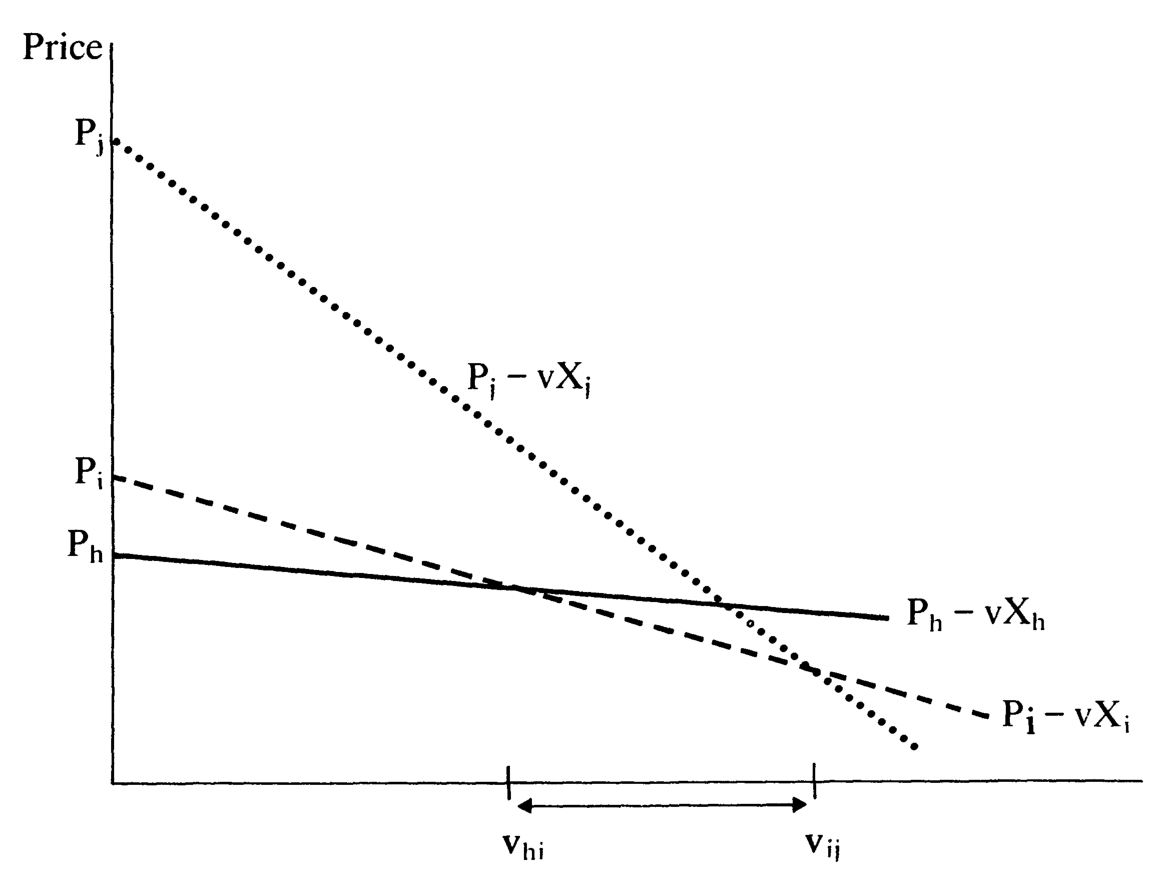
\includegraphics[width=\linewidth]{figures/ch06/bresnahan1987_fig1.png}
\caption{Total price lines in Bresnahan's form}
\end{subfigure}
\caption{Utility lines and cutoffs in the vertical model. (a) The utility $u_j(\nu) = \delta_j - \nu p_j$ of each
product is a line with intercept $\delta_j$ and slope $-p_j$, and the outside good is the horizontal axis.
The products are those of \cref{fig:06-frontier}. The bold upper envelope gives the chosen product, and
adjacent lines cross at the cutoffs $\bar\nu_3 < \bar\nu_2 < \bar\nu_1$, here $0.42$, $0.8$ and $1.6$. The
strip below the axis shows the product chosen on each interval of $\nu$. The dashed gray line is product
$b$, which never reaches the envelope. (b) The same construction in the form
$\frac{u_{ij}}{\nu_i} = v_i\delta_j - p_j$ used by \citet{Bresnahan1987}. A consumer with taste for quality
$v = \frac{1}{\nu}$ buys the product with the lowest total price $P - vX$, where Bresnahan writes $P$ for price and $X$ for
quality. Product $i$ is bought on the
marked interval $[v_{hi}, v_{ij}]$. Because $v$ is the reciprocal of $\nu$, the order of products along the
horizontal axis is reversed. Source: Bresnahan (1987), Figure 1.}
\label{fig:06-ulines}
\end{figure}

Without the frontier assumption, the same logic gives a single formula that holds for any qualities
\citep[eqs.~14--17]{BerryPakes2007}. Keep all products ordered by price, but let qualities be arbitrary.
Product $j$ beats product $k$ if and only if $\nu(p_j - p_k) < \delta_j - \delta_k$. For a cheaper product
$k < j$, dividing by $p_j - p_k > 0$ gives $\nu < \frac{\delta_j - \delta_k}{p_j - p_k}$. For a more expensive
product $k > j$, dividing by $p_j - p_k < 0$ reverses the inequality and gives
$\nu > \frac{\delta_k - \delta_j}{p_k - p_j}$. Product $j$ is chosen if and only if
$\underline\nu_j(\delta, p) < \nu < \bar\nu_j(\delta, p)$, where
\begin{equation}\label{eq:06-bp-cutoffs}
  \bar\nu_j(\delta, p) = \min_{k < j} \frac{\delta_j - \delta_k}{p_j - p_k}, \qquad
  \underline\nu_j(\delta, p) = \max_{k > j} \frac{\delta_k - \delta_j}{p_k - p_j},
\end{equation}
with the conventions $\bar\nu_0(\delta, p) = \infty$ and $\underline\nu_J(\delta, p) = 0$. The share of
product $j$ is
\begin{equation}\label{eq:06-bp-share}
  s_j = \big[F(\bar\nu_j(\delta, p)) - F(\underline\nu_j(\delta, p))\big]\,
        \indic\big\{\bar\nu_j(\delta, p) > \underline\nu_j(\delta, p)\big\}.
\end{equation}
\citet{BerryPakes2007} write these cutoffs as $\overline\Delta_j$ and $\underline\Delta_j$ and the price
sensitivity as $\alpha_i$.

\begin{remark}[General and adjacent cutoffs]\label{rem:06-general-cutoffs}
Formula \eqref{eq:06-bp-share} has three useful properties. First, for a product on the frontier,
$\bar\nu_j(\delta,p) = \bar\nu_j$ and $\underline\nu_j(\delta,p) = \bar\nu_{j+1}$, the adjacent cutoffs of
\eqref{eq:06-cutoff}. The slope of the chord from $j$ back to a cheaper frontier product $k$ is an average
of the edge slopes $\bar\nu_{k+1}, \dots, \bar\nu_j$. Each of these is at least $\bar\nu_j$, so the minimum is
attained at $k = j - 1$. Points below the frontier give chords at least as steep, so they do not change the minimum.
The same argument applies to the maximum. Second, the formula assigns a zero share to every product off the
frontier, so one expression serves for every parameter value. This matters in estimation, where a trial
parameter value can reorder qualities. Third, the vertical model predicts exact zero shares for some
parameter values, which models with an idiosyncratic shock never do. Since observed shares are positive,
the true parameters must place every product with positive sales on the frontier. Deleting the products
dominated outright is not enough to impose this. Product $b$ in \cref{fig:06-frontier} beats every cheaper
product in quality and still sells nothing.
\end{remark}

\subsection{Market shares}\label{sec:06-vshares}

Integrating the choice intervals over the taste distribution gives the demand system.

\begin{proposition}[Vertical market shares]\label{prop:06-vshares}
Under \cref{ass:06-vertical}, with all $J$ products on the frontier, the market shares are
\begin{equation}\label{eq:06-vshares}
  s_j = F(\bar\nu_j) - F(\bar\nu_{j+1}), \quad j = 1, \dots, J, \qquad
  s_0 = 1 - F(\bar\nu_1) = 1 - F\Big(\frac{\delta_1}{p_1}\Big),
\end{equation}
with $F(\bar\nu_{J+1}) = F(0) = 0$. Quantities are $q_j = M s_j$.
\end{proposition}

\begin{proof}
By \cref{prop:06-cutoffs}, $s_j = \Pr(\bar\nu_{j+1} < \nu_i < \bar\nu_j)$. Since $F$ is continuous, the end points
carry no mass, and $s_j = F(\bar\nu_j) - F(\bar\nu_{j+1})$. For the outside good, $s_0 = \Pr(\nu_i > \bar\nu_1) =
1 - F(\bar\nu_1)$. For the top product, $s_J = F(\bar\nu_J) - F(0) = F(\bar\nu_J)$. Summing over
$j = 0, \dots, J$ telescopes to one.
\end{proof}

Four features of \eqref{eq:06-vshares} recur below. Shares depend on qualities and prices only through
the $J$ cutoffs. The share of product $j$ depends only on its own price and the prices of its two
neighbors. The outside share depends only on the price and quality of the cheapest product. Zero shares
are possible, for any product off the frontier. \Cref{fig:06-nuaxis} draws the shares as areas under the
density.

\begin{figure}[htbp]
\centering
\begin{tikzpicture}
\begin{axis}[
  width=0.8\textwidth, height=5.6cm,
  xmin=0, xmax=3.05, ymin=0, ymax=1.12,
  axis lines=left,
  xlabel={price sensitivity $\nu$}, ylabel={$f(\nu)$},
  xtick={0.416667,0.8,1.6}, xticklabels={$\bar\nu_3$,$\bar\nu_2$,$\bar\nu_1$},
  ytick={0,0.5,1},
  clip=false,
]
  \addplot[name path=dens, thick, domain=0:3, samples=150] {exp(-x)};
  \path[name path=base] (axis cs:0,0) -- (axis cs:3,0);
  \addplot[fill=blue!45] fill between[of=dens and base, soft clip={domain=0:0.416667}];
  \addplot[fill=blue!28] fill between[of=dens and base, soft clip={domain=0.416667:0.8}];
  \addplot[fill=blue!14] fill between[of=dens and base, soft clip={domain=0.8:1.6}];
  \addplot[fill=gray!18] fill between[of=dens and base, soft clip={domain=1.6:3}];
  \draw[thin] (axis cs:0.416667,0) -- (axis cs:0.416667,{exp(-0.416667)});
  \draw[thin] (axis cs:0.8,0) -- (axis cs:0.8,{exp(-0.8)});
  \draw[thin] (axis cs:1.6,0) -- (axis cs:1.6,{exp(-1.6)});
  \node at (axis cs:0.2,0.33) {$s_3$};
  \node at (axis cs:0.61,0.25) {$s_2$};
  \node at (axis cs:1.2,0.15) {$s_1$};
  \node at (axis cs:2.05,0.06) {$s_0$};
  \node[anchor=west] at (axis cs:1.0,0.75) {$f(\nu) = e^{-\nu}$};
\end{axis}
\end{tikzpicture}
\caption{Market shares as areas under the taste density. The density is exponential with mean one, and the
cutoffs are those of \cref{fig:06-ulines}, $\bar\nu_3 = 0.42$, $\bar\nu_2 = 0.8$ and $\bar\nu_1 = 1.6$. The least
price-sensitive consumers buy the top product. The shares are $s_3 = 0.341$, $s_2 = 0.210$, $s_1 = 0.247$
and $s_0 = 0.202$.}
\label{fig:06-nuaxis}
\end{figure}

\begin{example}[Uniform tastes for quality]\label{ex:06-uniform}
\citet{Bresnahan1987} works with the form \eqref{eq:06-vertical-v} and assumes that the taste for quality
$v_i = \frac{1}{\nu_i}$ is uniform on $[0, \bar v]$ with density $\kappa$, so the market has $M = \kappa\bar v$
consumers.\footnote{Bresnahan writes quality as $x$, the taste density as $\delta$, and the upper bound
as $V_{\max}$. We write $\delta_j$, $\kappa$ and $\bar v$ to keep the notation of this chapter.} In
$v$-space the cutoff between $j-1$ and $j$ is the reciprocal of \eqref{eq:06-cutoff},
\begin{equation*}
  v_{j-1,j} = \frac{1}{\bar\nu_j} = \frac{p_j - p_{j-1}}{\delta_j - \delta_{j-1}},
\end{equation*}
and consumers with $v > v_{j-1,j}$ prefer $j$ \citep[eq.~4]{Bresnahan1987}. The implied CDF of
$\nu = \frac{1}{v}$ is
\begin{equation*}
  F(\nu) = \Pr\Big(v \ge \frac{1}{\nu}\Big) = 1 - \frac{1}{\bar v\,\nu}, \qquad \nu \ge \frac{1}{\bar v},
\end{equation*}
and zero below $\frac{1}{\bar v}$. Substituting into \eqref{eq:06-vshares},
\begin{equation*}
  s_j = \Big[1 - \frac{1}{\bar v\,\bar\nu_j}\Big] - \Big[1 - \frac{1}{\bar v\,\bar\nu_{j+1}}\Big]
      = \frac{1}{\bar v}\big(v_{j,j+1} - v_{j-1,j}\big),
\end{equation*}
so that $q_j = M s_j = \kappa\,(v_{j,j+1} - v_{j-1,j})$, or
\begin{equation}\label{eq:06-vuniform-demand}
  q_j = \kappa\Big[\frac{p_{j+1} - p_j}{\delta_{j+1} - \delta_j} - \frac{p_j - p_{j-1}}{\delta_j - \delta_{j-1}}\Big],
  \qquad
  q_J = \kappa\Big[\bar v - \frac{p_J - p_{J-1}}{\delta_J - \delta_{J-1}}\Big].
\end{equation}
These are equations (10) and (11) of \citet{Bresnahan1987}. Demand is linear in prices because the
cutoffs in $v$-space are linear in prices. The support of $\nu$ starts at $\frac{1}{\bar v}$ instead of
zero, so the top product sells only if $v_{J-1,J} < \bar v$. Bresnahan assumes that the consumer with the
highest taste, $\bar v$, always buys a car. In his application the alternative to a new car is a used
car of quality $\delta_{\mathrm u}$ and price $p_{\mathrm u}$, which replaces the origin as the point
$(p_0, \delta_0)$ (\cref{sec:06-vext}).
\end{example}

\subsection{Inverting market shares}\label{sec:06-vinversion}

Estimation requires the reverse map, from observed shares to qualities (\cref{sec:06-inversion-idea}). In
the vertical model the inverse exists, is unique, and has a closed form. Let
\begin{equation}\label{eq:06-cumshare}
  S_j = \sum_{k \ge j} s_k, \qquad j = 1, \dots, J,
\end{equation}
be the \emph{cumulative share from the top}, the share of consumers who buy product $j$ or a more
expensive product.

\begin{proposition}[Inversion]\label{prop:06-vinversion}
Under \cref{ass:06-vertical}, let the prices satisfy $0 < p_1 < \dots < p_J$ and let the observed shares
$s_j = \frac{q_j}{M}$ be positive for $j = 1, \dots, J$, with $s_0 = 1 - \sum_j s_j > 0$. There is exactly
one quality vector $\delta$ under which all $J$ products lie on the frontier and the predicted shares
\eqref{eq:06-vshares} equal the observed shares. It is given by
\begin{align}
  \bar\nu_j &= F^{-1}(S_j), \label{eq:06-vinv-cut}\\
  \delta_j &= \delta_{j-1} + (p_j - p_{j-1})\,F^{-1}(S_j), \qquad \delta_0 = 0, \label{eq:06-vinv-rec}\\
  \delta_j &= \sum_{m=1}^{j} (p_m - p_{m-1})\, F^{-1}\Big(\sum_{k \ge m} s_k\Big). \label{eq:06-vinv-sum}
\end{align}
\end{proposition}

\begin{proof}
The first step sums shares from the top. Under \eqref{eq:06-vshares},
\begin{equation*}
  S_j = \sum_{k=j}^{J} \big[F(\bar\nu_k) - F(\bar\nu_{k+1})\big] = F(\bar\nu_j) - F(\bar\nu_{J+1}) = F(\bar\nu_j).
\end{equation*}
The second step proves uniqueness. Because $F$ is continuous and strictly increasing on $(0,\infty)$, its
inverse $F^{-1}$ is well defined on $(0,1)$. Each $S_j$ lies in $(0,1)$, since $s_J > 0$ and
$1 - S_1 = s_0 > 0$. Hence $\bar\nu_j = F^{-1}(S_j)$ is the only cutoff consistent with the data. The
definition \eqref{eq:06-cutoff} gives $\delta_j - \delta_{j-1} = (p_j - p_{j-1})\bar\nu_j$, which is
\eqref{eq:06-vinv-rec}. Starting from $\delta_0 = 0$ and iterating gives \eqref{eq:06-vinv-sum}, so every
quality is pinned down.

The third step proves existence. Define $\delta$ by \eqref{eq:06-vinv-sum}. All shares are positive, so
$S_1 > S_2 > \dots > S_J > 0$. Because $F^{-1}$ is strictly increasing, $\bar\nu_1 > \bar\nu_2 > \dots > \bar\nu_J
> 0$. Qualities then increase with price and the cutoffs decrease, so by \cref{prop:06-frontier} every
product lies on the frontier. \Cref{prop:06-vshares} gives predicted shares
$F(\bar\nu_j) - F(\bar\nu_{j+1}) = S_j - S_{j+1} = s_j$.
\end{proof}

Several consequences follow. The price ordering determines the quality ordering, so the data reveal the
ranking of products without any parameter. Every vector of positive shares is rationalized by some quality
vector, whatever the increasing distribution $F$. A single market's prices and shares therefore never
reject the vertical model. Its testable content comes from restrictions across products and markets, such
as $\delta_{jt} = x_{jt}\beta + \xi_{jt}$, and from the supply side.

The result is an instance of the general invertibility theory of \citet{BerryGandhiHaile2013}. On the set
of qualities at which every product sells, raising $\delta_j$ raises $\bar\nu_j$ and lowers $\bar\nu_{j+1}$.
It therefore raises $s_j$, lowers $s_{j-1}$ and $s_{j+1}$ (or $s_0$ when $j = 1$), and leaves every other
share unchanged. Inside goods are weak substitutes in this sense. The chain $0, 1, \dots, J$ of strict
substitution between neighbors connects every inside good to the outside good. These are the ``connected
substitutes'' conditions under which \citet{BerryGandhiHaile2013} prove that demand is invertible. The
proof above exploits the special structure and also delivers the inverse in closed form.

Market size enters through every share. Holding unit sales fixed, a larger $M$ lowers every cumulative
share $S_j$, which lowers every cutoff and every quality. A market with more nonbuyers is rationalized by
products that are worse relative to the outside good. The choice of $M$ is an assumption, and it
matters for the level of the recovered qualities.

\begin{example}[Exponential tastes]\label{ex:06-exponential}
Let $F(\nu) = 1 - e^{-\lambda\nu}$ with $\lambda > 0$, so that $\E[\nu_i] = \frac{1}{\lambda}$. Solving
$u = 1 - e^{-\lambda\nu}$ for $\nu$ gives
\begin{equation*}
  F^{-1}(u) = -\frac{1}{\lambda}\ln(1 - u).
\end{equation*}
Substituting into \eqref{eq:06-vinv-sum},
\begin{equation}\label{eq:06-vexp-delta}
  \delta_j = -\frac{1}{\lambda}\sum_{m=1}^{j}(p_m - p_{m-1})\ln(1 - S_m),
  \qquad 1 - S_m = s_0 + \sum_{l < m} s_l ,
\end{equation}
where $1 - S_m$ is the share of consumers who buy the outside good or a product cheaper than $m$. Now let
there be markets $t = 1, \dots, T$, and let $(m)$ denote the $m$-th cheapest product of market $t$. For the
product $j$ that occupies position $k$ in market $t$, define the observable
\begin{equation}\label{eq:06-vexp-y}
  y_{jt} \equiv -\sum_{m=1}^{k}\big(p_{(m)t} - p_{(m-1)t}\big)\ln(1 - S_{mt}),
\end{equation}
which uses prices and shares only. By \eqref{eq:06-vexp-delta}, $y_{jt} = \lambda\delta_{jt}$. Substituting
$\delta_{jt} = x_{jt}\beta + \xi_{jt}$ gives the estimable equation
\begin{equation}\label{eq:06-vexp-reg}
  y_{jt} = x_{jt}(\lambda\beta) + \lambda\xi_{jt} .
\end{equation}
\end{example}

\begin{proposition}[Scale of tastes]\label{prop:06-vscale}
In \cref{ex:06-exponential}, $\lambda$ is not identified. For every $c > 0$ the parameters
$(\lambda, \beta, \xi)$ and $(\frac{\lambda}{c}, c\beta, c\xi)$ imply the same choice for every consumer and
hence the same shares. More generally, for any $F$, the pairs $(F(\cdot), \delta)$ and
$(F(\frac{\cdot}{c}), c\delta)$ are observationally equivalent.
\end{proposition}

\begin{proof}
Let $\nu$ have CDF $F$ and define $\nu' = c\nu$. Then $\Pr(\nu' \le x) = \Pr(\nu \le \frac{x}{c}) = F(\frac{x}{c})$.
A consumer of type $\nu$ facing qualities $\delta$ compares $\delta_j - \nu p_j$ across products. Multiplying
by $c > 0$ gives
\begin{equation*}
  c\delta_j - (c\nu)p_j = c\delta_j - \nu' p_j ,
\end{equation*}
which ranks products in the same order. So a consumer of type $\nu'$ facing qualities $c\delta$ makes the
same choice as a consumer of type $\nu$ facing $\delta$. Integrating over types, the shares under
$(F(\frac{\cdot}{c}), c\delta)$ equal those under $(F, \delta)$. For the exponential distribution,
$F(\frac{x}{c}) = 1 - e^{-\frac{\lambda}{c}x}$ is exponential with parameter $\frac{\lambda}{c}$, and
$c\delta_j = x_j(c\beta) + c\xi_j$.
\end{proof}

The economic content is that choices reveal quality only in units of willingness to pay. Doubling every
quality and doubling every consumer's price sensitivity describes the same consumers making the same
choices. This is the scale normalization of \cref{sec:06-normalization} in the vertical model. We set
$\lambda = 1$, so that $\E[\nu_i] = 1$. A consumer with the mean price sensitivity then values one unit of
quality at one dollar, and \eqref{eq:06-vexp-reg} becomes $y_{jt} = x_{jt}\beta + \xi_{jt}$.

With $\lambda = 1$ the demand parameters are identified under two conditions. The first is the moment
condition $\E[x_{jt}^\top\xi_{jt}] = 0$, and the second is full rank of $\E[x_{jt}^\top x_{jt}]$. Then
$\beta = \E[x_{jt}^\top x_{jt}]^{-1}\E[x_{jt}^\top y_{jt}]$, and the OLS regression of $y_{jt}$ on $x_{jt}$ is
consistent. Price is not a regressor. It enters only the construction of $y_{jt}$, an exact function of
observed prices and shares. Firms that observe $\xi_{jt}$ set higher prices for better products, so
$p_{jt}$ and $\xi_{jt}$ are correlated. This correlation does not bias the regression, because the vertical
model has no price coefficient left to estimate. The normalized distribution $F$ plays the role of the
price coefficient. It states how many consumers have each price sensitivity, and nothing about it remains
unknown. Standard errors should be clustered by market. The values $y_{jt}$ of products in the same market
are built from the same cumulative shares. Any sampling error in observed shares, or any misspecification of $F$,
therefore enters the errors of all products in a market and accumulates along the price ladder.

The same feature is the model's main weakness. With $F$ fully specified, every substitution pattern is
determined by functional form and by the observed prices and shares (\cref{prop:06-vmarkup-data} below).
Exogenous variation in prices is never used to learn how demand responds to prices. Two further cautions
apply. The moment condition fails if firms choose characteristics with knowledge of $\xi_{jt}$
(\cref{sec:06-charspace}). If $F$ is misspecified, $y_{jt}$ differs from $\delta_{jt}$ by a function of
prices and shares, and the regression error inherits that function.

\begin{remark}[Shape parameters and instruments]\label{rem:06-vshape}
Suppose that after the scale normalization $F$ still has an unknown shape parameter. An example is
$\ln\nu_i \sim N(0, \sigma^2)$, whose median is fixed at one. With $\Phi$ the standard normal CDF,
$F_\sigma^{-1}(u) = \exp(\sigma\Phi^{-1}(u))$, and the inversion gives
\begin{equation*}
  \delta_{jt}(\sigma) = \sum_{m=1}^{k}\big(p_{(m)t} - p_{(m-1)t}\big)\exp\big(\sigma\,\Phi^{-1}(S_{mt})\big).
\end{equation*}
For any trial value of $\sigma$, OLS of $\delta_{jt}(\sigma)$ on $x_{jt}$ produces residuals orthogonal to
$x_{jt}$. The $K$ moments $\E[x_{jt}^\top\xi_{jt}] = 0$ therefore cannot determine the $K + 1$ parameters
$(\beta, \sigma)$. Identification of $\sigma$ requires at least one excluded instrument $z_{jt}$. This is a variable
uncorrelated with $\xi_{jt}$ that moves prices or shares, such as a cost shifter or a characteristic of
rival products. Stack the instruments in $Z_{jt} = (x_{jt}, z_{jt})$ and define
$\xi_{jt}(\sigma, \beta) = \delta_{jt}(\sigma) - x_{jt}\beta$. The GMM estimator uses
$\E[Z_{jt}^\top\xi_{jt}(\sigma,\beta)] = 0$. For fixed $\sigma$ the estimate of $\beta$ is the linear IV
estimator
\begin{equation*}
  \hat\beta(\sigma) = (X^\top Z W Z^\top X)^{-1} X^\top Z W Z^\top\delta(\sigma),
\end{equation*}
where $X$, $Z$ and $\delta(\sigma)$ stack the observations and $W$ is a weighting matrix. Concentrating out
$\beta$ leaves a search over $\sigma$ alone,
\begin{equation*}
  \hat\sigma = \argmin_{\sigma}\; g_N(\sigma)^\top W g_N(\sigma), \qquad
  g_N(\sigma) = \frac{1}{N}\sum_{j,t} Z_{jt}^\top\big(\delta_{jt}(\sigma) - x_{jt}\hat\beta(\sigma)\big).
\end{equation*}
This is the structure of the estimator for the nonlinear parameters $\theta_2$ in \cref{ch:blp}. Price
endogeneity now matters. Prices enter $\delta_{jt}(\sigma)$ in a way that depends on $\sigma$, so the
instruments must move prices independently of $\xi_{jt}$. Standard errors are again clustered by market.
\end{remark}

The uniform model of \cref{ex:06-uniform} inverts in the same way. Summing \eqref{eq:06-vuniform-demand} from
the top gives $\sum_{k \ge j} q_k = \kappa(\bar v - v_{j-1,j})$. Dividing by $M = \kappa\bar v$ gives
$v_{j-1,j} = \bar v(1 - S_j)$, so
\begin{equation*}
  \delta_j - \delta_{j-1} = \frac{p_j - p_{j-1}}{\bar v(1 - S_j)} .
\end{equation*}
Given the market size, $\bar v$ only sets the units of quality, in line with \cref{prop:06-vscale}.

\subsection{Substitution patterns}\label{sec:06-vsubst}

We now hold qualities fixed and differentiate shares with respect to prices. Each price enters only the
two cutoffs that involve its product. Differentiating \eqref{eq:06-cutoff},
\begin{align*}
  \frac{\partial\bar\nu_j}{\partial p_j} &= -\frac{\delta_j - \delta_{j-1}}{(p_j - p_{j-1})^2} = -\frac{\bar\nu_j}{p_j - p_{j-1}},
  &
  \frac{\partial\bar\nu_j}{\partial p_{j-1}} &= \frac{\delta_j - \delta_{j-1}}{(p_j - p_{j-1})^2} = \frac{\bar\nu_j}{p_j - p_{j-1}},
\end{align*}
and, shifting the index,
\begin{equation*}
  \frac{\partial\bar\nu_{j+1}}{\partial p_j} = \frac{\bar\nu_{j+1}}{p_{j+1} - p_j},
  \qquad
  \frac{\partial\bar\nu_{j+1}}{\partial p_{j+1}} = -\frac{\bar\nu_{j+1}}{p_{j+1} - p_j}.
\end{equation*}
A higher own price lowers the upper cutoff of $j$ and raises its lower cutoff, so the interval of buyers
shrinks from both ends. It is convenient to define
\begin{equation}\label{eq:06-gj}
  g_j = f(\bar\nu_j)\,\frac{\bar\nu_j}{p_j - p_{j-1}} > 0, \quad j = 1, \dots, J, \qquad g_{J+1} = 0 .
\end{equation}
The number $g_j$ is the density of consumers at the boundary between $j - 1$ and $j$, times the speed at
which that boundary moves when either price changes.

\begin{proposition}[Price derivatives]\label{prop:06-vderiv}
Under \cref{ass:06-vertical}, with all products on the frontier and qualities held fixed,
\begin{align}
  \frac{\partial s_j}{\partial p_j} &= -g_j - g_{j+1}
     = -\frac{f(\bar\nu_j)\bar\nu_j}{p_j - p_{j-1}} - \frac{f(\bar\nu_{j+1})\bar\nu_{j+1}}{p_{j+1} - p_j}, \label{eq:06-vown}\\
  \frac{\partial s_j}{\partial p_{j-1}} &= g_j, \qquad \frac{\partial s_j}{\partial p_{j+1}} = g_{j+1}, \qquad
  \frac{\partial s_j}{\partial p_k} = 0 \ \text{ for } |k - j| \ge 2, \label{eq:06-vcross}\\
  \frac{\partial s_0}{\partial p_1} &= g_1, \qquad \frac{\partial s_0}{\partial p_k} = 0 \ \text{ for } k \ge 2.
  \label{eq:06-voutside}
\end{align}
The second term of \eqref{eq:06-vown} is absent for the top product. The $J \times J$ Jacobian $\Delta^s$ with
$\Delta^s_{jk} = \frac{\partial s_j}{\partial p_k}$ is tridiagonal and symmetric, with
$\Delta^s_{j,j+1} = \Delta^s_{j+1,j} = g_{j+1}$. Each column of the $(J+1) \times J$ matrix that adds the outside-good
row sums to zero.
\end{proposition}

\begin{proof}
Write $s_j = F(\bar\nu_j) - F(\bar\nu_{j+1})$. The price $p_j$ enters $\bar\nu_j$ and $\bar\nu_{j+1}$ only, so by the
chain rule
\begin{equation*}
  \frac{\partial s_j}{\partial p_j} = f(\bar\nu_j)\frac{\partial\bar\nu_j}{\partial p_j} - f(\bar\nu_{j+1})\frac{\partial\bar\nu_{j+1}}{\partial p_j}
  = -f(\bar\nu_j)\frac{\bar\nu_j}{p_j - p_{j-1}} - f(\bar\nu_{j+1})\frac{\bar\nu_{j+1}}{p_{j+1} - p_j}.
\end{equation*}
The price $p_{j-1}$ enters $s_j$ only through $\bar\nu_j$, so $\frac{\partial s_j}{\partial p_{j-1}} =
f(\bar\nu_j)\frac{\bar\nu_j}{p_j - p_{j-1}} = g_j$. The price $p_{j+1}$ enters $s_j$ only through $\bar\nu_{j+1}$,
so
\begin{equation*}
  \frac{\partial s_j}{\partial p_{j+1}} = -f(\bar\nu_{j+1})\frac{\partial\bar\nu_{j+1}}{\partial p_{j+1}}
  = f(\bar\nu_{j+1})\frac{\bar\nu_{j+1}}{p_{j+1} - p_j} = g_{j+1}.
\end{equation*}
No other price enters $s_j$. For the outside good, $s_0 = 1 - F(\bar\nu_1)$ with $\bar\nu_1 = \frac{\delta_1}{p_1}$,
so $\frac{\partial s_0}{\partial p_1} = f(\bar\nu_1)\frac{\bar\nu_1}{p_1} = g_1$. Symmetry follows by comparing
$\Delta^s_{j,j+1} = g_{j+1}$ with $\Delta^s_{j+1,j} = \frac{\partial s_{j+1}}{\partial p_j} = g_{j+1}$, the second identity
in \eqref{eq:06-vcross} applied to product $j+1$. Column $k$ has the entries $g_k$ in row $k - 1$ (the outside
row when $k = 1$), $-g_k - g_{k+1}$ in row $k$, and $g_{k+1}$ in row $k + 1$. They sum to zero.
\end{proof}

Symmetry has a simple reading. The number $g_{j+1}$ measures the consumers at the boundary between $j$
and $j + 1$. A small rise in $p_j$ moves these marginal consumers from $j$ to $j + 1$, and an equal rise in
$p_{j+1}$ moves the same consumers back. The flow across a shared boundary is the same in both directions.
Symmetry also follows from the envelope argument behind \cref{thm:06-wdz}. Dividing utility by $\nu_i$ gives
$\frac{u_{ij}}{\nu_i} = \frac{\delta_j}{\nu_i} - p_j$, which is quasi-linear in money for each consumer.
Aggregate consumer surplus $CS(p) = M\,\E\big[\max_j(\frac{\delta_j}{\nu_i} - p_j)\big]$ therefore satisfies
$\frac{\partial CS}{\partial p_j} = -q_j$, and the symmetry of its second derivatives gives
$\frac{\partial q_j}{\partial p_k} = \frac{\partial q_k}{\partial p_j}$. The zero column sums say that a price
change only reallocates the $M$ consumers among the alternatives.

The structure of $\Delta^s$ has further consequences used in \cref{sec:06-vpricing}. In row $j$ with
$2 \le j \le J$, the off-diagonal entries $g_j$ and $g_{j+1}$ sum to $|\Delta^s_{jj}|$. In the first row,
$|\Delta^s_{11}| = g_1 + g_2$ exceeds the single off-diagonal entry $g_2$, because product 1 also loses consumers
to the outside good. So $\Delta^s$ is weakly diagonally dominant, strictly so in the first row. Because $\Delta^s$ is
tridiagonal with nonzero off-diagonal entries, it is also irreducible. An irreducible matrix that is weakly
diagonally dominant with at least one strictly dominant row is nonsingular \citep[ch.~6]{BermanPlemmons1994}.
\Cref{lem:06-mmatrix} in \cref{sec:06-bres-equilibrium} states and proves this fact in the form we need.

The \emph{diversion ratio} from $j$ to $k$ is the fraction of the consumers lost by $j$ after a price
increase who switch to $k$ (\cref{ch:diffprod}). We write it $D_{jk} = -\frac{\Delta^s_{kj}}{\Delta^s_{jj}}$. Here
\begin{equation*}
  D_{j,j-1} = \frac{g_j}{g_j + g_{j+1}}, \qquad
  D_{j,j+1} = \frac{g_{j+1}}{g_j + g_{j+1}},
\end{equation*}
and all other diversion ratios are zero. Every consumer who leaves $j$ goes to a price neighbor, with the
outside good counting as the lower neighbor of product 1.

We write the elasticity of the share of $j$ with respect to the price of $k$ as
$\varepsilon_{jk} = \frac{\partial s_j}{\partial p_k}\frac{p_k}{s_j}$. The diagonal entries are negative, and the
own-price elasticity in the positive convention of the book is $\varepsilon_j = -\varepsilon_{jj} =
\frac{(g_j + g_{j+1})p_j}{s_j}$. The outside good has the single nonzero elasticity
$\varepsilon_{01} = \frac{g_1 p_1}{s_0}$.

Closeness in price means closeness in substitution. Holding a cutoff fixed, the cross derivative
$g_{j+1} = f(\bar\nu_{j+1})\frac{\bar\nu_{j+1}}{p_{j+1} - p_j}$ grows without bound as $p_{j+1} - p_j \to 0$, and the
own derivatives of both products grow with it. In the data the cutoff is pinned down by shares through
$\bar\nu_{j+1} = F^{-1}(S_{j+1})$. Two products that sell at nearly the same price are therefore read as
near-perfect substitutes, whatever the products are. With uniform tastes the derivatives are constant.
Using $f(\nu) = \frac{1}{\bar v\nu^2}$ from \cref{ex:06-uniform},
\begin{equation*}
  M g_j = \kappa\bar v\cdot\frac{1}{\bar v\,\bar\nu_j^2}\cdot\frac{\bar\nu_j}{p_j - p_{j-1}}
        = \frac{\kappa}{\bar\nu_j(p_j - p_{j-1})} = \frac{\kappa}{\delta_j - \delta_{j-1}} .
\end{equation*}
Hence $\frac{\partial q_j}{\partial p_j} = -\kappa\big(\frac{1}{\delta_j - \delta_{j-1}} + \frac{1}{\delta_{j+1} - \delta_j}\big)$
and $\frac{\partial q_{j\pm1}}{\partial p_j} = \frac{\kappa}{|\delta_{j\pm1} - \delta_j|}$. Demand is linear, and the
quality gap measures how close two products are. In Bresnahan's words, the products are perfect
substitutes ``in the limit as $x_i$ goes to $x_h$,'' where $x$ is his notation for quality
\citep[p.~462]{Bresnahan1987}.

Is this a reasonable model of substitution? The restriction that only price neighbors substitute is
strong. A price cut on a mid-size sedan has no effect on a model two steps away on the price ladder,
however similar the two cars are physically. Conversely, a minivan and a sports car at the same price are
treated as close substitutes because they are neighbors on the ladder. The restriction is natural where
quality is essentially one-dimensional, as with airline cabins or storage tiers. It is also the source of
the power of the conduct test in \cref{sec:06-bresnahan}. Where products differ along several dimensions,
it can mislead badly.

A simulated illustration shows how badly (\cref{app:problems}). Market data are generated by a random
coefficients logit model in 100 markets, each offering between four and nine of ten products. The vertical
model with exponential tastes and $\lambda = 1$ is then fitted to these data. In one market the fitted own-price
elasticities $\varepsilon_{jj}$ range from $-358.4$ to $-16.8$, while the true $\varepsilon_{jj}$ range from $-3.85$
to $-2.57$. The largest
elasticities belong to products whose price neighbor sells at almost the same price. The two products with the
largest elasticities in that market are price neighbors whose prices differ by only 0.019. Across all markets, the median gap between
adjacent prices is 0.057, and 58 of the 554 gaps are below 0.01. The vertical model can explain why
consumers split across products with similar prices only by placing those products almost on top of each
other in quality. Under multi-product Nash pricing it then implies a mean markup of 0.048, against a true
mean markup of 0.386.

\subsection{Pricing and recovering marginal costs}\label{sec:06-vpricing}

Firms indexed by $f$ own disjoint sets of products $\mathcal J_f$ and produce at constant marginal costs
$mc_j$. Firm
$f$ chooses the prices of its products to maximize $M\sum_{k \in \mathcal J_f}(p_k - mc_k)s_k(p)$. The
first-order condition for $p_j$, $j \in \mathcal J_f$, is
\begin{equation*}
  s_j + \sum_{k \in \mathcal J_f}(p_k - mc_k)\frac{\partial s_k}{\partial p_j} = 0 .
\end{equation*}
With the ownership matrix $\Omega$ ($\Omega_{jk} = 1$ if $j$ and $k$ have the same owner) and $\odot$ the
element-wise product, the conditions stack into
\begin{equation}\label{eq:06-vfoc-matrix}
  s + (\Omega \odot \Delta^{s\top})(p - mc) = 0
  \qquad\Longrightarrow\qquad
  mc = p + (\Omega \odot \Delta^{s\top})^{-1}s ,
\end{equation}
the multi-product markup formula of \cref{ch:diffprod}. By \cref{prop:06-vderiv}, the condition for product
$j$ involves only its neighbors. Writing $m_j = p_j - mc_j$ for the markup,
\begin{equation}\label{eq:06-vfoc}
  s_j - (g_j + g_{j+1})\,m_j + \Omega_{j,j+1}\,g_{j+1}\,m_{j+1} + \Omega_{j,j-1}\,g_j\,m_{j-1} = 0,
\end{equation}
with $\Omega_{1,0} = 0$ because the outside good earns no markup. A single-product firm sets
$m_j = \frac{s_j}{g_j + g_{j+1}}$, which is the inverse elasticity rule $\frac{m_j}{p_j} = \frac{1}{\varepsilon_j}$.
Equation \eqref{eq:06-vfoc} is the general-$F$ version of the conduct equation that \citet{Bresnahan1987}
estimates (\cref{sec:06-bresnahan}).

\begin{corollary}[Only neighbors' ownership matters]\label{cor:06-neighbors}
Under the conditions of \cref{prop:06-vderiv}, the matrix $\Omega \odot \Delta^{s\top}$ is block diagonal. Each
block corresponds to a maximal run of consecutive products with the same owner. Two ownership structures
that agree on which adjacent pairs share an owner imply the same first-order conditions, and hence the
same markups and implied marginal costs. Moreover, $\Omega \odot \Delta^{s\top}$ is nonsingular, and the markups
$m = -(\Omega \odot \Delta^{s\top})^{-1}s$ are positive.
\end{corollary}

\begin{proof}
Because $\Delta^{s\top}$ is tridiagonal, $(\Omega \odot \Delta^{s\top})_{jk} = \Omega_{jk}\Delta^s_{kj}$ vanishes unless $|j - k| \le 1$.
For $|j - k| = 1$ it equals $g_{\max\{j,k\}}$ if the two products share an owner and zero otherwise. So the
matrix depends on $\Omega$ only through the entries $\Omega_{j,j+1}$, and it breaks into blocks at every
adjacent pair with different owners. Within a block that starts at product $a$, the first row has diagonal
entry $-(g_a + g_{a+1})$ and off-diagonal entry $g_{a+1}$, so it is strictly diagonally dominant by
$g_a > 0$. The other rows are weakly dominant, as in the discussion after \cref{prop:06-vderiv}. Each block
is tridiagonal with nonzero off-diagonal entries, hence irreducible. The negative of each block therefore
has a positive diagonal, nonpositive off-diagonal entries, nonnegative row sums and a strictly positive
first row sum. By \cref{lem:06-mmatrix}(a) it is a nonsingular M-matrix whose inverse has positive entries. Since $s > 0$, the markups $m = \big(-(\Omega \odot \Delta^{s\top})\big)^{-1}s$ are
positive.
\end{proof}

The corollary is a sharp prediction. A firm that owns products 1 and 3 but not product 2 prices exactly
as two independent firms would. Joint ownership raises markups only when it links products that
compete for the same marginal consumers.

The vertical model has a second, more surprising property. When $F$ is known up to scale, the markups
require no demand estimate at all.

\begin{proposition}[Markups from prices and shares]\label{prop:06-vmarkup-data}
Under \cref{ass:06-vertical}, suppose $F(\nu) = F_1(\lambda\nu)$ for a known CDF $F_1$ with density $f_1$
and an unknown scale $\lambda > 0$. Then the Jacobian $\Delta^s$, the markups $-(\Omega \odot \Delta^{s\top})^{-1}s$ and the
implied marginal costs depend only on observed prices and shares. They depend on no demand parameter,
including $\lambda$ and $\beta$. With exponential tastes,
\begin{equation}\label{eq:06-vexp-g}
  \bar\nu_j = -\frac{1}{\lambda}\ln(1 - S_j), \qquad f(\bar\nu_j) = \lambda(1 - S_j), \qquad
  g_j = \frac{-(1 - S_j)\ln(1 - S_j)}{p_j - p_{j-1}} .
\end{equation}
\end{proposition}

\begin{proof}
By \cref{prop:06-vinversion}, $\bar\nu_j = F^{-1}(S_j) = \frac{1}{\lambda}F_1^{-1}(S_j)$. The density is
$f(\nu) = \lambda f_1(\lambda\nu)$. Hence
\begin{equation*}
  f(\bar\nu_j)\,\bar\nu_j = \lambda f_1\big(F_1^{-1}(S_j)\big)\cdot\frac{1}{\lambda}F_1^{-1}(S_j)
  = f_1\big(F_1^{-1}(S_j)\big)\,F_1^{-1}(S_j),
\end{equation*}
and $g_j = \frac{f_1(F_1^{-1}(S_j))F_1^{-1}(S_j)}{p_j - p_{j-1}}$ depends on prices and shares only.
\Cref{prop:06-vderiv} builds $\Delta^s$ from the $g_j$, and \eqref{eq:06-vfoc-matrix} builds the markups and
marginal costs from $\Delta^s$, $s$ and $p$. For the exponential case, $F_1(x) = 1 - e^{-x}$, so
$F_1^{-1}(u) = -\ln(1 - u)$ and $f_1(F_1^{-1}(u)) = e^{\ln(1-u)} = 1 - u$.
\end{proof}

The scale drops out for a reason. Markups are measured in dollars, while the scale normalization concerns
the units of utility, so no choice of units can change them. The proposition has two practical
consequences. First, the supply side can be estimated without any demand estimate. The implied marginal
cost of each product is a known function of the data. Second, demand and supply share no parameter. When
the demand error $\xi_{jt}$ and the cost error $\omega_{jt}$ are independent, estimating the two equations
separately loses no efficiency. The flip side is the caution raised in \cref{sec:06-vinversion}. The
model reads market power off the spacing of prices and the cumulative shares, never off exogenous price
variation.

The supply equations take two forms, one per conduct assumption. Under marginal-cost pricing,
\begin{equation}\label{eq:06-vsupply-mc}
  p_{jt} = x_{jt}\gamma_1 + \gamma_2 z_{jt} + \omega_{jt} .
\end{equation}
Under multi-product Nash pricing,
\begin{equation}\label{eq:06-vsupply-nash}
  p_{jt} + \big[(\Omega_t \odot \Delta_t^{s\top})^{-1}s_t\big]_j = x_{jt}\gamma_1 + \gamma_2 z_{jt} + \omega_{jt} .
\end{equation}
Here $z_{jt}$ is a cost shifter excluded from demand, and $\gamma_1$ and $\gamma_2$ are cost coefficients,
unrelated to Euler's constant $\gamma_E$. Under either assumption the left side is data, so OLS under
$\E[\omega_{jt} \mid x_{jt}, z_{jt}] = 0$ estimates the cost parameters. The conduct assumption determines how
large the markup is, and so how much of the price variation across products is attributed to cost.
Comparing the two specifications is the logic of the conduct test in \cref{sec:06-bresnahan}.

\begin{remark}[Existence of a price equilibrium]\label{rem:06-vexist}
\citet[footnote~6]{Bresnahan1987} observes that a price equilibrium always exists in quality models of
this kind, while it can fail in location models. With uniform tastes, consider product $j$ as its own price
falls. Its interval of buyers widens, and at some price the next product $j + 1$ is dominated out of the
market. Demand for $j$ stays continuous at that price, because the interval of $j + 1$ shrinks continuously
to zero. The slope of demand changes from $-\kappa\big(\frac{1}{\delta_{j+1} - \delta_j} + \frac{1}{\delta_j - \delta_{j-1}}\big)$
to $-\kappa\big(\frac{1}{\delta_{j+2} - \delta_j} + \frac{1}{\delta_j - \delta_{j-1}}\big)$. The second is smaller in
absolute value, because $\delta_{j+2} - \delta_j > \delta_{j+1} - \delta_j$. So demand is flatter below the kink
than above it, and the derivative $\frac{\partial q_j}{\partial p_j}$ falls as $p_j$ rises. Demand is concave in own
price across the kink, and the same holds where the lower neighbor drops out. Profit $(p_j - mc_j)q_j$ is
then concave in $p_j$ on the range of prices at which $j$ sells with a positive markup, and it is zero beyond
that range. Profit is therefore quasi-concave, and standard fixed-point arguments give an equilibrium. In the Hotelling model with linear costs, demand jumps when a firm captures the rival's
location, and existence can fail (\cref{sec:06-hotelling}). \citet[Theorem~2]{CaplinNalebuff1991} cover general taste
densities with single-product firms. Utility must be linear in the taste parameter, as in \eqref{eq:06-vertical-v}
with type $v_i$. The density of $v_i$ must be $\rho$-concave with $\rho = -\frac{1}{2}$, the case $n = 1$ of their
assumption A2. This means that $\frac{1}{\sqrt{f}}$ is convex, a condition that every log-concave density meets
(\cref{sec:06-branches} and \cref{ch:diffprod}).
\end{remark}

\begin{example}[A worked example]\label{ex:06-vnumeric}
Three products and an outside good face exponential tastes with $\lambda = 1$. Observed prices are
$p = (1.0, 1.5, 2.5)$ and observed shares are $s = (0.20, 0.15, 0.10)$, so $s_0 = 0.55$. \Cref{tab:06-vnumeric}
reports every step, computed to more digits than shown.

The first step inverts the shares. Cumulative shares are $S = (0.45, 0.25, 0.10)$. By \eqref{eq:06-vexp-g},
the cutoffs are $\bar\nu_1 = -\ln 0.55 = 0.598$, $\bar\nu_2 = -\ln 0.75 = 0.288$ and $\bar\nu_3 = -\ln 0.90 = 0.105$.
They decrease, as \cref{prop:06-vinversion} guarantees, so all three products are on the frontier. The
recursion \eqref{eq:06-vinv-rec} gives
\begin{align*}
  \delta_1 &= 1.0 \times 0.598 = 0.598,\\
  \delta_2 &= 0.598 + 0.5 \times 0.288 = 0.742,\\
  \delta_3 &= 0.742 + 1.0 \times 0.105 = 0.847 .
\end{align*}
Recomputing the shares at these qualities with \eqref{eq:06-bp-share} returns the observed shares
exactly. Simulating two million consumers returns them up to simulation error.

The second step computes substitution. The densities at the cutoffs are $f(\bar\nu_j) = 1 - S_j = (0.55, 0.75,
0.90)$. Formula \eqref{eq:06-gj} gives $g_1 = \frac{0.55 \times 0.598}{1.0} = 0.329$, $g_2 = \frac{0.75 \times 0.288}{0.5}
= 0.432$ and $g_3 = \frac{0.90 \times 0.105}{1.0} = 0.095$. These fill the Jacobian through
\cref{prop:06-vderiv}. Product 2 has the most elastic demand, $\varepsilon_2 = 5.26$. It sits between two
neighbors, and its lower neighbor is only 0.5 away in price. Product 3, at the top, has a single
neighbor and the least elastic demand, $\varepsilon_3 = 2.37$. The outside good responds only to $p_1$.

The third step backs out markups and marginal costs under three ownership structures, holding the observed
prices and shares fixed. Under (a) single-product firms, $m_j = \frac{s_j}{g_j + g_{j+1}}$, which gives
markups of $0.263$, $0.285$ and $1.055$. Under (b) joint ownership of products 1 and 2, the boundary between
them, where $g_2 = 0.432$ is large, is internalized. The implied markups of 1 and 2 roughly triple to
$0.794$ and $0.936$. The markup of product 3 is unchanged at $1.055$, since its own first-order condition
does not change. Under (c) a single owner of all three products, the implied markups are $1.369$, $1.948$
and $3.002$. They exceed the prices, so the implied marginal costs are negative. The observed prices are
too low to be monopoly prices under this demand system, and conduct (c) is rejected by the requirement
that costs be nonnegative. Finally, joint ownership of products 1 and 3 alone reproduces the numbers of
case (a) to every digit, as \cref{cor:06-neighbors} predicts.
\end{example}

\begin{table}[htbp]
\centering
\caption{Worked example of the vertical model with exponential tastes}\label{tab:06-vnumeric}
\small
\begin{tabular}{@{}lrrrrrrr@{}}
\toprule
\multicolumn{8}{@{}l}{\emph{Panel A. Inversion}}\\
Product $j$ & $p_j$ & $s_j$ & $S_j$ & $\bar\nu_j$ & $f(\bar\nu_j)$ & $\delta_j$ & $g_j$ \\
\midrule
1 & 1.0 & 0.20 & 0.45 & 0.598 & 0.55 & 0.598 & 0.329 \\
2 & 1.5 & 0.15 & 0.25 & 0.288 & 0.75 & 0.742 & 0.432 \\
3 & 2.5 & 0.10 & 0.10 & 0.105 & 0.90 & 0.847 & 0.095 \\
\midrule
\multicolumn{8}{@{}l}{\emph{Panel B. Share derivatives $\frac{\partial s_j}{\partial p_k}$ and elasticities $\varepsilon_{jk}$}}\\
 & \multicolumn{3}{c}{Derivative with respect to} & & \multicolumn{3}{c}{Elasticity with respect to}\\
\cmidrule(lr){2-4}\cmidrule(lr){6-8}
 & $p_1$ & $p_2$ & $p_3$ & & $p_1$ & $p_2$ & $p_3$ \\
\midrule
Product 1    & $-0.760$ & $0.432$  & $0$      & & $-3.802$ & $3.236$  & $0$ \\
Product 2    & $0.432$  & $-0.526$ & $0.095$  & & $2.877$  & $-5.263$ & $1.580$ \\
Product 3    & $0$      & $0.095$  & $-0.095$ & & $0$      & $1.422$  & $-2.371$ \\
Outside good & $0.329$  & $0$      & $0$      & & $0.598$  & $0$      & $0$ \\
\midrule
\multicolumn{8}{@{}l}{\emph{Panel C. Implied markups $m_j$ and marginal costs $mc_j$ at the observed prices}}\\
 & \multicolumn{3}{c}{Markup $m_j$} & & \multicolumn{3}{c}{Marginal cost $mc_j$}\\
\cmidrule(lr){2-4}\cmidrule(lr){6-8}
Ownership & 1 & 2 & 3 & & 1 & 2 & 3 \\
\midrule
(a) Single-product firms   & 0.263 & 0.285 & 1.055 & & 0.737 & 1.215 & 1.445 \\
(b) Products 1 and 2 joint & 0.794 & 0.936 & 1.055 & & 0.206 & 0.564 & 1.445 \\
(c) One firm owns all      & 1.369 & 1.948 & 3.002 & & $-0.369$ & $-0.448$ & $-0.502$ \\
\bottomrule
\end{tabular}
\par\smallskip
\begin{minipage}{0.95\textwidth}
\footnotesize Notes: Tastes are exponential with $\lambda = 1$ and the outside share is $s_0 = 0.55$. In Panel A,
$S_j = \sum_{k \ge j} s_k$, $\bar\nu_j = -\ln(1 - S_j)$, $f(\bar\nu_j) = 1 - S_j$, $\delta_j$ follows \eqref{eq:06-vinv-rec},
and $g_j$ follows \eqref{eq:06-gj}. In Panel B, rows are shares and columns are prices, and
$\varepsilon_{jk} = \frac{\partial s_j}{\partial p_k}\frac{p_k}{s_j}$. In Panel C, $m = -(\Omega \odot \Delta^{s\top})^{-1}s$ and
$mc = p - m$. Joint ownership of products 1 and 3 gives the numbers of row (a).
\end{minipage}
\end{table}

\subsection{Extensions}\label{sec:06-vext}

The basic model extends in several directions that the rest of the chapter uses.

\begin{remark}[An outside alternative with quality]\label{rem:06-vext-used}
The outside good need not sit at the origin. In the market for new cars, a consumer who buys no new car
keeps or buys a used car. \citet[eq.~2]{Bresnahan1987} gives this alternative a quality $\delta_{\mathrm u}$
and a price $p_{\mathrm u}$, so the outside option is the point $(p_{\mathrm u}, \delta_{\mathrm u})$ of the
$(p,\delta)$ plane. Every result of this section goes through with $(p_0, \delta_0) = (p_{\mathrm u},
\delta_{\mathrm u})$. The lowest cutoff becomes $\bar\nu_1 = \frac{\delta_1 - \delta_{\mathrm u}}{p_1 - p_{\mathrm u}}$,
and in Bresnahan's form the demand for the lowest-quality new car is
\begin{equation*}
  q_1 = \kappa\Big[\frac{p_2 - p_1}{\delta_2 - \delta_1} - \frac{p_1 - p_{\mathrm u}}{\delta_1 - \delta_{\mathrm u}}\Big]
\end{equation*}
\citep[eq.~9]{Bresnahan1987}. In Bresnahan's words, ``it is exactly as if there were some other `product'
below the lowest-quality product'' \citep[p.~463]{Bresnahan1987}.
\end{remark}

\begin{remark}[Quality measured with error]\label{rem:06-vext-error}
Suppose consumers know each product's quality but the econometrician observes only a noisy proxy,
$\delta_j = \delta(x_j) + \eta_j$ with $\eta_j$ unobserved. Each consumer still substitutes only between price
neighbors. The demand predicted by the econometrician, averaged over $\eta$, depends on several neighbors,
because the frontier itself is uncertain. Measurement error in quality thus spreads substitution across
more products, a step toward random coefficients models. \Cref{sec:06-bresnahan} uses this device as a
robustness check.
\end{remark}

\begin{remark}[Income heterogeneity]\label{rem:06-vext-income}
In the specification $u_{ij} = \delta_j(y_i - p_j)$ of \citet{GabszewiczThisse1979}, the type is income.
\Cref{sec:06-vdef} shows that the cutoff between $j - 1$ and $j$ is the income
$\frac{\delta_j p_j - \delta_{j-1}p_{j-1}}{\delta_j - \delta_{j-1}}$. With an income distribution in place of
$F$, shares, the inversion and the derivatives follow the same steps, with higher incomes buying higher
qualities.
\end{remark}

\begin{remark}[A building block for the pure characteristics model]\label{rem:06-vext-pc}
Let $u_{ij} = x_j\beta_i - \alpha_i p_j + \xi_j$ with random coefficients $\beta_i$ on the characteristics and
$\alpha_i$ on price. Conditional on $\beta_i$, this is a vertical model in the price sensitivity $\alpha_i$,
with qualities $x_j\beta_i + \xi_j$. Shares are therefore a mixture of vertical shares
\eqref{eq:06-bp-share} over the distribution of $\beta_i$ \citep[eq.~18]{BerryPakes2007}. The general
cutoffs \eqref{eq:06-bp-cutoffs} are essential here, because the frontier changes with $\beta_i$.
\Cref{sec:06-bp-shares} develops the computation.
\end{remark}

\begin{remark}[Natural oligopolies]\label{rem:06-vext-ss}
When firms choose qualities before prices, vertical differentiation limits the number of firms that can
survive. A duopoly example of \citet[sec.~7.5.1]{Tirole1988}, which follows \citet{GabszewiczThisse1979}
and \citet{ShakedSutton1982}, shows the mechanism. Utility is $v\delta_j - p_j$, with $v$ uniform on
$[\underline v, \bar v]$ and $\bar v = \underline v + 1$. Both firms have unit cost $c$, qualities satisfy
$\delta_1 < \delta_2$, and $h = \delta_2 - \delta_1$. Suppose qualities are high enough that every consumer
buys. The type indifferent between the two products is $v^* = \frac{p_2 - p_1}{h}$, so
$q_1 = v^* - \underline v$ and $q_2 = \bar v - v^*$. The first-order conditions for maximizing
$(p_1 - c)q_1$ and $(p_2 - c)q_2$ are
\begin{equation*}
  p_1 = \frac{p_2 + c - \underline v h}{2}, \qquad p_2 = \frac{p_1 + c + \bar v h}{2} .
\end{equation*}
Substituting the second condition into the first and solving gives
\begin{equation*}
  p_1 - c = \frac{(\bar v - 2\underline v)h}{3}, \qquad p_2 - c = \frac{(2\bar v - \underline v)h}{3},
\end{equation*}
with quantities $q_1 = \frac{\bar v - 2\underline v}{3}$ and $q_2 = \frac{2\bar v - \underline v}{3}$. Profits are
\begin{equation*}
  \pi_1 = \frac{(\bar v - 2\underline v)^2 h}{9}, \qquad \pi_2 = \frac{(2\bar v - \underline v)^2 h}{9} .
\end{equation*}
Both profits rise with the quality gap $h$. If qualities are chosen at no cost from a fixed interval
before prices are set, the two firms therefore locate at its two ends. The low-quality firm sells a
positive quantity only if $\bar v > 2\underline v$. When $\bar v \le 2\underline v$, consumers are too similar,
and price competition drives the low-quality firm from the market even though entry is free. \citet{ShakedSutton1983} generalize this force into a
\emph{finiteness result}. Suppose that every consumer would buy the highest quality if all qualities sold at unit
cost. Then only a bounded number of firms can have positive market shares, however large the market
becomes. The condition requires that unit costs not rise too quickly with quality. It is more likely to hold
when the cost of quality falls mainly on research and development or other fixed costs. Tirole contrasts the result with the Salop model, in which the number of firms grows without bound
as fixed costs fall.
\end{remark}

\section{Case study: the 1955 automobile price war}\label{sec:06-bresnahan}

The vertical model entered empirical industrial organization through a study of conduct.
\citet{Bresnahan1987} asks whether the American automobile boom of 1955 was a price war. The paper embeds the
vertical model of \cref{sec:06-vertical} in an oligopoly model with multi-product firms. It solves the model under
two conduct hypotheses, collusion and Bertrand-Nash competition, and estimates each version by maximum likelihood
for the model years 1954, 1955 and 1956. Non-nested tests then ask which hypothesis the data favor in each year. No
cost data enter. Conduct is identified from the fine structure of the cross-section of products. What matters is
which products are close neighbors in quality, and whether a close neighbor belongs to the same firm or to a rival.

The section follows the order of a full case study. We state the question and the facts
(\cref{sec:06-bres-question,sec:06-bres-facts}), describe the data (\cref{sec:06-bres-data}), and set out the
model (\cref{sec:06-bres-model}). We then prove the equilibrium properties on which the test rests. Markups rise
whenever a pair of neighbors starts to cooperate, collusive markups have a closed form, and Bertrand markups of
close rivals vanish. Estimation, the non-nested test, the estimates, the counterfactual and the robustness checks
follow (\cref{sec:06-bres-estimation,sec:06-bres-cox,sec:06-bres-estimates,sec:06-bres-fit,sec:06-bres-robust}).
The section closes with identification, critiques and the contribution of the paper
(\cref{sec:06-bres-ident,sec:06-bres-limits,sec:06-bres-contribution}).

\subsection{The question and why it matters}\label{sec:06-bres-question}

In the 1955 model year, American passenger car production was about 45 percent higher than in the two
surrounding years, while quality-adjusted prices were lower \citep[p.~457]{Bresnahan1987}. Aggregate demand models
fit that year poorly. \citet[pp.~168--169]{Chow1960}, a leading study of automobile demand, reports that ``the
year 1955 is an exception'' to the rule of small residuals. Its 1955 residual is ``twice as large as the standard
error'' (quoted in \citealp[footnote~1]{Bresnahan1987}). Paul Samuelson stated the puzzle more
sharply. He ``would flunk any econometrics paper that claimed to provide an explanation of 1955 auto
sales.''\footnote{Bresnahan reports the classroom remark and attributes the anecdote to Robert E. Hall
\citep[footnote~2]{Bresnahan1987}.}

Higher output at a lower price is the signature of a supply shift. A pure demand shock moves the market along an
upward-sloping supply relation and raises price, so it cannot produce a price trough in a boom on its own.
Bresnahan therefore looks for a supply shock, and he proposes one of a specific form. His hypothesis is a one-year
breakdown of tacit collusion among the automakers. Under this hypothesis firms priced to maximize joint profits in
the 1954 and 1956 model years and competed in prices in the 1955 model year. The 1955 boom was then, in part, a
price war.

The paper matters for three reasons. First, it is the first structural test of conduct in a differentiated-products
industry, and it works without any data on costs. \citet[p.~844]{BerryLevinsohnPakes1995} call it ``perhaps the
first attempt at simultaneously modeling and estimating the demand and oligopoly pricing sides of the market.''
Conduct is encoded in a cooperation matrix $\Omega$, the same object that merger simulation changes when two firms
combine (\cref{ch:mergers}). Second, it shows that conduct can change over time within one industry. This links it
to the empirical study of collusion (\cref{ch:collusion-evidence}), where \citet{Porter1983} documents switches
between collusive and non-collusive periods in a railroad cartel from time-series data. Bresnahan instead uses the
cross-section of products within each year.

Third, a price war in a boom year speaks to theories of collusion over the business cycle
(\cref{ch:collusion-theory}). In \citet{RotembergSaloner1986}, collusion is hardest to sustain when current demand
is high relative to future demand, so collusive prices fall in booms. They read Bresnahan's results as support for
their theory, because 1955 was a boom year.\footnote{The 1984 NBER working-paper version of
\citet{RotembergSaloner1986} discusses Bresnahan's study in its section on evidence.} In
\citet{GreenPorter1984}, by contrast, price wars follow unexpectedly low demand. The 1955 episode fits the first
theory better. Bresnahan does not test either theory. His contribution is to show that the conduct of 1955 differed
from that of the neighboring years. He later judged that such evidence had not separated the theories, and he doubted that further studies of the
same kind would. Rotemberg and
Saloner combine the regime switches that \citet{Porter1983} reports with the pattern of conduct that
\citet{Bresnahan1987} finds. \citet[p.~1025]{Bresnahan1989} sees ``little in these investigations that
differentiates among the various theories.'' The timing of changes in conduct is harder to estimate than its
average level. A study of what starts and ends price wars has as many observations as there are price wars, far
fewer than the number of periods.

\subsection{Setting and aggregate facts}\label{sec:06-bres-facts}

The American industry of the mid-1950s consisted of three large firms, General Motors (GM), Ford and Chrysler, and
a fringe of smaller producers that included American Motors (AMC). Firms sell several models each. The time unit
is the \emph{model year}: the row labelled 1955 in the tables covers the fourth quarter of 1954 through the third
quarter of 1955. Bresnahan treats the model year as a short run in a precise sense. Within it, firms set prices and
quantities, but their product lines are predetermined. With fixed costs of product development, products are
imperfect substitutes in equilibrium. Even the ``competitive'' model therefore has market power. The label refers
to noncooperative conduct. Even competing firms are not price takers \citep[p.~458]{Bresnahan1987}.

\begin{table}[htbp]
\centering
\caption{Aggregate indicators of the automobile market, model years 1953--1957}
\label{tab:06-bres-facts}
\small
\begin{tabular}{@{}lrrrrr@{}}
\toprule
 & 1953 & 1954 & 1955 & 1956 & 1957 \\
\midrule
\multicolumn{6}{@{}l}{\textit{Automobile market (Bresnahan's Table I)}} \\
(1) Production, millions of units & 6.13 & 5.51 & 7.94 & 5.80 & 6.12 \\
(2) Real price: CPI for new cars relative to the CPI & 1.01 & 0.99 & 0.95 & 0.97 & 0.98 \\
(3) Quality-adjusted price (Cagan), percent change & NA & NA & $-2.5$ & 6.3 & 6.1 \\
(4) Real sales, billions of 1957 dollars & 14.5 & 13.9 & 18.4 & 15.7 & 16.2 \\
(5) Quantity index, (4) divided by (2), 1957 $=100$ & 86.8 & 84.9 & 117.2 & 97.9 & 100.0 \\
\addlinespace
\multicolumn{6}{@{}l}{\textit{Outside the automobile market (Bresnahan's Table II)}} \\
(6) Per capita disposable personal income & 1623 & 1609 & 1659 & 1717 & 1732 \\
(7) Three-month Treasury bill rate, percent & 1.9 & 0.9 & 1.7 & 2.6 & 3.2 \\
(8) Non-auto durables spending, billions of 1957 dollars & 14.5 & 14.5 & 16.1 & 17.1 & 17.0 \\
(9) Accounting profits of the automakers & 2.58 & 2.25 & 3.91 & 2.21 & 2.38 \\
\bottomrule
\end{tabular}

\smallskip
\begin{minipage}{0.95\textwidth}
\footnotesize
\emph{Notes:} Reproduced from \citet[Tables I and II, p.~459]{Bresnahan1987}. Rows are model years. Nominal values
are deflated with the GNP deflator. Row (3) is the percentage change in Cagan's (1971) quality-adjusted price
index, which uses only physically unchanged models. Row (4) is auto output in constant dollars from the National
Income and Product Accounts. The source's note for row (6) reads ``billions of 1957 dollars'', which cannot apply to
a per capita figure. The values are 1957 dollars per person. Row (9) is the profit of the five largest automobile
companies. The note that should give its units is not printed in the source.
\end{minipage}
\end{table}

\Cref{tab:06-bres-facts} shows why 1955 is anomalous. Production jumped to 7.94 million cars. This is 44 percent
above 1954, 37 percent above 1956, and 40.4 percent above the average of the two years. Bresnahan's round figure of
45 percent is close to the comparison with 1954. At the same time the real
price of new cars hit its trough of 0.95. Quality adjustment does not change the picture. The quality-adjusted index
of \citet{Cagan1971} fell by 2.5 percent in 1955 and rose by 6.3 percent in 1956. Bresnahan notes that the hedonic
index of \citet{Griliches1964} behaves similarly.

Row (4) adds a second fact. Real sales in value terms rose by 32 percent between 1954 and 1955, much less than the
44 percent rise in units. The implicit quantity index of row (5) rose by more than real sales. Bresnahan reads this
as a one-year shift of buyers toward smaller, lower-value cars, and he points to production by price group in
\emph{Ward's Automotive Yearbook} (his footnote~3). The shift matters later, because the price war hypothesis
predicts that competition intensifies most in the small-car segment.

Rows (6) to (8) show that demand factors explain part of the boom. Per capita income rose by 3.1 percent in 1955.
The Treasury bill rate of 1.7 percent was below its 1956 and 1957 levels. Spending on other durables rose by 11
percent in 1955, but it did not fall in 1956, while automobile output collapsed. Bresnahan concludes that some of
the 1955 increase was due to demand, but that a full demand-side explanation would ``need to be fairly fancy''
\citep[p.~460]{Bresnahan1987}.

Row (9) invites a wrong inference. Accounting profits jumped from 2.25 to 3.91 in 1955, which seems to suggest
less competition. Automobile production, however, has large fixed costs for plant and product development. These
are joint costs of production over many years, and accounting practice spreads them smoothly over time. High-volume
years therefore look profitable in the accounting sense whatever happens to economic margins. There is no stable
time-series relation between accounting profits and price-cost margins. This is why Bresnahan estimates margins
from a structural model. His conclusion makes the general point that accounting-based measures of market power are
unsuitable for studies of single industries \citep[p.~479]{Bresnahan1987}.

Bresnahan calls the window of 1954 to 1956 ``not entirely arbitrary''.\footnote{Korean War price and quantity controls
were lifted in February and March 1953. Bresnahan dates the start of foreign competition ``of any consequence'' to
Volkswagen's entry in 1957. No labor-based work stoppage lasted more than ten days within the period
\citep[p.~472, footnote~13]{Bresnahan1987}. Volkswagen's own company history records that the Dutch
businessman Ben Pon brought two Volkswagen cars to New York in 1949. It also records that Volkswagen of America was
established in 1955 to organize dealers and provide parts and service \citep{VolkswagenHistory}. Bresnahan's 1957 date therefore marks the point at which imports became a consequential competitor. It is
later than the first sales of Volkswagen cars in the United States.} It starts after the end of wartime controls,
ends before foreign competition became consequential in his account, and contains no long strike. Each of the three
years is estimated separately, and no restriction links the parameters across years.

\subsection{Data and the quantity aggregation problem}\label{sec:06-bres-data}

The unit of observation is a physically distinct car model in a model year. Since demand elasticities in the model
are driven by quality differences between products, the definition of a product is central. Model names are not
useful for this purpose, because naming conventions vary across firms and over time.\footnote{Independent
manufacturers sometimes doubled the number of model names offered for sale with only trivial changes in the set of
physical products. Bresnahan notes that this was usually a warning sign of impending exit \citep[footnote~8]{Bresnahan1987}.}
Bresnahan treats two models as distinct in three cases. They are of different makes, they have different engines,
frames or body types, or they differ in weight or length by more than one percent. Pontiac and Chevrolet are different
makes in this sense, although GM produces both. Only hardtop and four-door sedan bodies enter, with two-door sedans
standing in for models without a four-door version. The result is about 80 to 85 models per year, against
140 to 150 at the finest possible disaggregation (pp.~468 and 480).

Prices are list prices in mid-April of the model year, the ``PA'' prices of \citet{OhtaGriliches1976}. Options are
excluded, except heaters where the information is available, and power steering and brakes are included only when
standard. No correction for dealer discounts is made, because the discount was constant across models before 1959.
List prices appear in tables in the three trade journals \emph{Ward's}, \emph{Automotive News} and
\emph{Automotive Industries}, and in the Company Pages of \emph{Ward's}. The \emph{Ward's} and \emph{Automotive News}
tables failed to match on about two percent of all prices. In every such case the other two sources gave a three-way
match \citep[p.~480]{Bresnahan1987}.

The physical characteristics are those of the hedonic study of \citet{OhtaGriliches1976}. They are length (bumper
to bumper, in thousands of inches), curb weight (in thousands of pounds), advertised maximum brake horsepower (in
hundreds), the number of cylinders, and a hardtop dummy. We collect them in the row vector $x_j$ of
\cref{sec:06-charspace}. Quantities are model-year production. They come from \emph{Automotive News},
\emph{Ward's} and \citet{Heasley1977}, with gaps filled from monthly production and the dates of model changeover.
Production ties each number to a physical product, but it does not correspond exactly to a market. Fleet sales and
end-of-year bargains, in particular, cannot be treated adequately.

Production is often reported more coarsely than the product definition. In the 1954 data, for example, Chrysler
reports production for the V-8 DeSoto, but both the Firedome and the Fireflite were sold with the V-8 engine. The
solution is to aggregate predicted quantities to the level of the data. Let observed quantities be indexed by
$m = 1,\dots,N_q$ and let $\mathcal I_m$ be the set of models whose production is reported jointly as $q_m$, with
$k_m = |\mathcal I_m|$ models in it. The residual for observation $m$ is
\begin{equation}\label{eq:06-bres-aggregation}
  q_m - \sum_{j\in\mathcal I_m} q_j^*,
\end{equation}
where $q_j^*$ is the model's prediction for model $j$. If each model's quantity error has variance $\sigma_q^2$
and errors are independent across models, the aggregated error has variance $k_m\sigma_q^2$. Coarser aggregation
thus produces heteroskedasticity of a known form, which the likelihood of \cref{sec:06-bres-estimation} handles by
weighting.

\subsection{The model}\label{sec:06-bres-model}

We write Bresnahan's model in the notation of this chapter. His quality $x$ is our $\delta$, and his physical
characteristics $z$ are our $x$. His taste density $\delta$ is our $\kappa$, and his upper endpoint $V_{\max}$ is our
$\bar v$. His used-car quality and price $(\gamma, E)$ are our $(\delta_{\mathrm u}, p_{\mathrm u})$. His
marginal-cost scale $\mu$ is our $\psi$, and his cooperation matrix $H$ is our $\Omega$. His number of models $n$ is
our $J$.

\begin{assumption}[Bresnahan's environment]\label{ass:06-bres}
\leavevmode
\begin{enumerate}[label=(\roman*)]
\item \emph{Unit demand.} Each consumer buys one new car or none. A consumer who buys no new car obtains a used car,
the outside option.
\item \emph{Utility.} A consumer with taste for quality $v$ and income $y$ obtains
\begin{equation}\label{eq:06-bres-utility}
\begin{aligned}
  u(\delta_j, y, v) &= v\,\delta_j + y - p_j &&\text{from new car } j,\\
  u(\delta_{\mathrm u}, y, v) &= v\,\delta_{\mathrm u} + y - p_{\mathrm u} &&\text{from the used car.}
\end{aligned}
\end{equation}
\item \emph{Tastes.} The taste $v$ is uniformly distributed on $[0,\bar v]$ with density $\kappa$. The number of
potential buyers is $M = \kappa\bar v$.
\item \emph{Costs.} Model $j$ costs $C(\delta_j, q_j) = FC(\delta_j) + mc(\delta_j)\,q_j$ with
$mc(\delta) = \psi e^{\delta}$ and $\psi > 0$. The fixed cost $FC(\delta_j)$ is sunk at the pricing stage.
\item \emph{Used-car price.} $p_{\mathrm u} = mc(\delta_{\mathrm u})$.
\item \emph{Product set.} Qualities are fixed and ordered, $\delta_{\mathrm u} < \delta_1 < \dots < \delta_J$, and the
last quality step costs less than the highest taste for quality,
$\frac{mc(\delta_J) - mc(\delta_{J-1})}{\delta_J - \delta_{J-1}} < \bar v$.
\end{enumerate}
\end{assumption}

Parts (i) to (iii) are the vertical model of \cref{ass:06-vertical}, except that the price sensitivity has support
$[\frac{1}{\bar v}, \infty)$ and the outside option is a used car, as we show below. Part (v) is a restriction that
Bresnahan imposes in estimation, because the used-car price and quality were hard to tell apart in the data
(p.~468). Part (vi) says that the consumer with the highest valuation of quality values the last quality step at
more than its cost. By convexity of $mc$, $\bar v > mc'(\delta_J)$ is a sufficient condition. Part (vi) guarantees
that every product sells when prices equal marginal costs.

\subsubsection{Demand}\label{sec:06-bres-demand}

A consumer of type $v$ buys the product with the lowest ``total price'' $p_j - v\delta_j$, since income enters
utility additively. Consider two products $h$ and $i$ with $\delta_i > \delta_h$. The consumer is indifferent when
\begin{equation*}
  p_i - v\,\delta_i = p_h - v\,\delta_h .
\end{equation*}
Solving for $v$ gives the cutoff type
\begin{equation}\label{eq:06-bres-cutoff}
  v_{hi} = \frac{p_i - p_h}{\delta_i - \delta_h},
\end{equation}
and every type above $v_{hi}$ strictly prefers the higher-quality product $i$. With products ordered by quality and
all of them on the frontier, product $j$ is bought by the types in $[v_{j-1,j}, v_{j,j+1}]$. The used car enters as
a product $0$ with quality $\delta_{\mathrm u}$ and price $p_{\mathrm u}$. Comparing the two utilities in
\eqref{eq:06-bres-utility} gives the cutoff $v_{01} = \frac{p_1 - p_{\mathrm u}}{\delta_1 - \delta_{\mathrm u}}$,
which has exactly the form of \eqref{eq:06-bres-cutoff}. At the top, the type $\bar v$ buys the best car. Multiplying
the length of each interval by the density $\kappa$ gives Bresnahan's demand system (his eqs.~9--11):
\begin{equation}\label{eq:06-bres-demand}
\begin{aligned}
  q_1 &= \kappa\left[\frac{p_2 - p_1}{\delta_2 - \delta_1} - \frac{p_1 - p_{\mathrm u}}{\delta_1 - \delta_{\mathrm u}}\right],\\
  q_j &= \kappa\left[\frac{p_{j+1} - p_j}{\delta_{j+1} - \delta_j} - \frac{p_j - p_{j-1}}{\delta_j - \delta_{j-1}}\right],
  \qquad 1 < j < J,\\
  q_J &= \kappa\left[\bar v - \frac{p_J - p_{J-1}}{\delta_J - \delta_{J-1}}\right].
\end{aligned}
\end{equation}
Demand is linear in prices. Bresnahan chose the uniform distribution for exactly this reason
\citep[p.~460]{Bresnahan1987}, and he credits the demand system to \citet{PrescottVisscher1977}.

\Cref{eq:06-bres-demand} is the vertical model of \cref{sec:06-vertical} in another parametrization. Dividing
utility \eqref{eq:06-bres-utility} by $v > 0$ gives $\delta_j - \frac{p_j}{v} + \frac{y}{v}$. The last term is common
to all options and drops out, so the consumer has price sensitivity $\nu = \frac{1}{v}$. The cutoff
\eqref{eq:06-bres-cutoff} is then the reciprocal $v_{j-1,j} = \frac{1}{\bar\nu_j}$ of the cutoff of \cref{sec:06-vcutoffs}.
\Cref{ex:06-uniform} derives the implied distribution $F(\nu) = 1 - \frac{1}{\bar v\nu}$ of the price sensitivity and
shows that \cref{prop:06-vshares} then reproduces the interior and top equations of \eqref{eq:06-bres-demand}. The
first equation is the used-car extension of \cref{rem:06-vext-used}. Besides the support of the price
sensitivity, two differences from \cref{sec:06-vertical} remain. The outside option has a quality $\delta_{\mathrm u}$ and a price $p_{\mathrm u}$ instead of the
normalization $\delta_0 = p_0 = 0$. The scale of quality is not a free normalization here, because quality also
enters marginal cost, as \cref{sec:06-bres-ident} explains.

Let $h_j = \delta_j - \delta_{j-1}$ be the quality gap below product $j$, with $h_1 = \delta_1 - \delta_{\mathrm u}$.
Differentiating \eqref{eq:06-bres-demand} gives constant derivatives:
\begin{equation}\label{eq:06-bres-deriv}
  \frac{\partial q_j}{\partial p_j} = -\kappa\Bigl(\frac{1}{h_j} + \frac{1}{h_{j+1}}\Bigr)\ (j<J),
  \qquad
  \frac{\partial q_J}{\partial p_J} = -\frac{\kappa}{h_J},
  \qquad
  \frac{\partial q_{j+1}}{\partial p_j} = \frac{\partial q_j}{\partial p_{j+1}} = \frac{\kappa}{h_{j+1}},
\end{equation}
and all other cross derivatives are zero. These are the derivatives of \cref{prop:06-vderiv} multiplied by the
market size. In the notation of \eqref{eq:06-gj}, uniform tastes give $Mg_j = \frac{\kappa}{h_j}$, as computed at the
end of \cref{sec:06-vsubst}. The number $g_j$ of the general model is thus inversely proportional to the quality
gap $h_j$. As in \cref{ch:diffprod}, we write $\Delta$ for the $J\times J$ matrix of quantity derivatives,
$\Delta_{jk} = \frac{\partial q_j}{\partial p_k}$. It is symmetric and tridiagonal, and it equals $M$ times the share
Jacobian $\Delta^s$ of \cref{sec:06-vsubst}.

The quality gap measures closeness. The diversion ratio from product $j$ to its upper neighbor is
\begin{equation*}
  D_{j,j+1} = \frac{\frac{\partial q_{j+1}}{\partial p_j}}{-\frac{\partial q_j}{\partial p_j}}
  = \frac{\frac{1}{h_{j+1}}}{\frac{1}{h_j} + \frac{1}{h_{j+1}}}
  = \frac{h_j}{h_j + h_{j+1}} .
\end{equation*}
Diversion goes mostly to the closer neighbor. As $h_{j+1} \to 0$, the own and cross derivatives both diverge and
their ratio tends to one in absolute value, so the two products become perfect substitutes
\citep[p.~462]{Bresnahan1987}. Demand is continuous in prices even where a product's interval shrinks to zero, and
a price equilibrium exists (\cref{rem:06-vexist}).

\subsubsection{Costs and conduct}\label{sec:06-bres-conduct}

The cost function $C(\delta,q) = FC(\delta) + mc(\delta)q$ has a fixed cost and a constant marginal cost at each
quality. Marginal cost must increase with quality. Otherwise the best product is also the cheapest to make, and only
it would be produced. Bresnahan also wants $mc$ convex. Consumers trade money for quality at a constant marginal
rate, so convex costs mean decreasing returns to spending on quality, which rules out degenerate equilibria (his
footnote~7). Convexity has a sharp implication in this model. Define the chord slopes
\begin{equation}\label{eq:06-bres-chord}
  \chi_j = \frac{mc(\delta_j) - mc(\delta_{j-1})}{\delta_j - \delta_{j-1}},\quad j = 1,\dots,J,
  \qquad mc(\delta_0) \equiv mc(\delta_{\mathrm u}) = p_{\mathrm u},
  \qquad \chi_{J+1} \equiv \bar v .
\end{equation}
At marginal-cost prices, the cutoff between $j-1$ and $j$ equals $\chi_j$. Strict convexity makes the chord slopes
increase, $\chi_1 < \chi_2 < \dots < \chi_J$, and \cref{ass:06-bres}(vi) gives $\chi_J < \bar v$.
Every product therefore sells at marginal-cost prices, with quantity
\begin{equation}\label{eq:06-bres-qmc}
  q_j(mc) = \kappa\,(\chi_{j+1} - \chi_j) > 0, \qquad j = 1,\dots,J .
\end{equation}
The exponential $mc(\delta) = \psi e^{\delta}$ is the simplest increasing and convex form with one parameter. It
follows the log-linear hedonic price equations of \citet{OhtaGriliches1976}.

Each model earns $\pi_j = (p_j - mc_j)q_j - FC(\delta_j)$, where $mc_j = mc(\delta_j)$. Bresnahan considers two
conduct hypotheses. Under \emph{collusion} (C), all firms set prices to maximize the sum of all profits, as a single
monopolist would. Under \emph{Bertrand-Nash competition} (B), each firm sets the prices of its own models to
maximize its own profit, taking rivals' prices as given. Bresnahan's tables call the second hypothesis
``Nash-Competition'' or ``Bertrand''. Because demand links only neighbors, conduct enters through the relation
between each model and its two neighbors.

Consider first a model whose neighbors do not cooperate with it. Its owner sets the derivative of $\pi_j$ with
respect to $p_j$ to zero (his eq.~15):
\begin{equation}\label{eq:06-bres-foc-single}
  q_j + (p_j - mc_j)\frac{\partial q_j}{\partial p_j} = 0
  \quad\Longleftrightarrow\quad
  p_j - mc_j = \frac{q_j}{-\frac{\partial q_j}{\partial p_j}} .
\end{equation}
The markup equals quantity divided by the absolute slope of the model's own demand curve. If instead $j$ and $j+1$
cooperate, because one firm makes both or because firms collude, the price of $j$ also accounts for the profit of
$j+1$ (his eq.~16):
\begin{equation}\label{eq:06-bres-foc-coop}
  q_j + (p_j - mc_j)\frac{\partial q_j}{\partial p_j} + (p_{j+1} - mc_{j+1})\frac{\partial q_{j+1}}{\partial p_j} = 0 .
\end{equation}
The extra term is the effect of $j$'s price on its neighbor's profit. It is large when the two products are close,
since $\frac{\partial q_{j+1}}{\partial p_j} = \frac{\kappa}{h_{j+1}}$. This is why changing the conduct hypothesis
has large effects where products are closely spaced.

The \emph{cooperation matrix} $\Omega$ records which products cooperate (his eq.~17):
\begin{equation}\label{eq:06-bres-omega}
  \Omega_{jk} = \begin{cases} 1 & \text{if products } j \text{ and } k \text{ cooperate},\\
  0 & \text{otherwise.}\end{cases}
\end{equation}
It is symmetric with ones on the diagonal. Under Bertrand it is the ownership matrix of \cref{sec:06-vpricing}.
Under collusion every entry is one. In Bresnahan's three-product example, GM makes products 1 and 2 and Chrysler
makes product 3 (his eqs.~18--19):
\begin{equation}\label{eq:06-bres-omega-ex}
  \Omega^{\mathrm B} = \begin{pmatrix} 1 & 1 & 0\\ 1 & 1 & 0\\ 0 & 0 & 1\end{pmatrix},
  \qquad
  \Omega^{\mathrm C} = \begin{pmatrix} 1 & 1 & 1\\ 1 & 1 & 1\\ 1 & 1 & 1\end{pmatrix}.
\end{equation}
With this notation the first-order condition for every model takes one form (his eq.~20):
\begin{equation}\label{eq:06-bres-foc}
  0 = q_j + (p_j - mc_j)\frac{\partial q_j}{\partial p_j}
      + \Omega_{j,j+1}(p_{j+1} - mc_{j+1})\frac{\partial q_{j+1}}{\partial p_j}
      + \Omega_{j,j-1}(p_{j-1} - mc_{j-1})\frac{\partial q_{j-1}}{\partial p_j},
\end{equation}
where terms that refer to products outside $1,\dots,J$ are absent. The used car has an exogenous price and no
first-order condition. Solving the demand system \eqref{eq:06-bres-demand} together with the $J$ conditions
\eqref{eq:06-bres-foc} gives the equilibrium (his eq.~21)
\begin{equation}\label{eq:06-bres-eqm}
  p^* = p^*(\delta, \Omega, \delta_{\mathrm u}, \bar v, \kappa, \psi),
  \qquad
  q^* = q^*(\delta, \Omega, \delta_{\mathrm u}, \bar v, \kappa, \psi).
\end{equation}
Because demand is linear, profits are quadratic in prices and the first-order conditions are linear.

\subsubsection{The equilibrium as a linear system}\label{sec:06-bres-equilibrium}

The linear structure lets us prove the properties on which Bresnahan's test rests. Write $m_j = p_j - mc_j$ for the
markup of model $j$ and $m = (m_1,\dots,m_J)^\top$. We substitute $p_j = mc_j + m_j$ into \eqref{eq:06-bres-demand}.
Each quantity splits into its value at marginal-cost prices and a term in markups,
\begin{equation*}
  q_j = \kappa\Bigl[\frac{(mc_{j+1} - mc_j) + (m_{j+1} - m_j)}{h_{j+1}}
        - \frac{(mc_j - mc_{j-1}) + (m_j - m_{j-1})}{h_j}\Bigr],
\end{equation*}
where $m_0 = 0$ because $p_{\mathrm u} = mc(\delta_{\mathrm u})$. For $j = J$ the first term is replaced by
$\kappa\bar v$. Using \eqref{eq:06-bres-chord} and \eqref{eq:06-bres-deriv}, this is
\begin{equation*}
  q = q(mc) + \Delta\,m .
\end{equation*}
The first-order conditions \eqref{eq:06-bres-foc} read $q_j + \sum_k \Omega_{jk}\Delta_{kj}m_k = 0$, or
$q + (\Omega\odot \Delta^\top)m = 0$ in the notation of \cref{sec:06-vpricing}. Since $\Delta$ is symmetric, substituting
$q = q(mc) + \Delta m$ gives
\begin{equation}\label{eq:06-bres-linear}
  A(\Omega)\,m = q(mc),
  \qquad
  A(\Omega) = -\bigl(\Delta + \Omega\odot \Delta\bigr).
\end{equation}
The entries of $A(\Omega)$ are
\begin{equation}\label{eq:06-bres-Amat}
  A_{jj} = 2\kappa\Bigl(\frac{1}{h_j} + \frac{1}{h_{j+1}}\Bigr)\ (j < J),
  \qquad A_{JJ} = \frac{2\kappa}{h_J},
  \qquad A_{j,j+1} = A_{j+1,j} = -\bigl(1 + \Omega_{j,j+1}\bigr)\frac{\kappa}{h_{j+1}},
\end{equation}
and all other entries are zero. The diagonal does not depend on $\Omega$ because $\Omega_{jj} = 1$. Only the
neighbor entries $\Omega_{j,j+1}$ matter. The row sums are
\begin{equation}\label{eq:06-bres-rowsums}
\begin{aligned}
  \textstyle\sum_k A_{1k} &= \frac{2\kappa}{h_1} + \bigl(1 - \Omega_{12}\bigr)\frac{\kappa}{h_2} > 0,\\
  \textstyle\sum_k A_{jk} &= \bigl(1 - \Omega_{j-1,j}\bigr)\frac{\kappa}{h_j} + \bigl(1 - \Omega_{j,j+1}\bigr)\frac{\kappa}{h_{j+1}} \ge 0,
  \qquad 1 < j < J,\\
  \textstyle\sum_k A_{Jk} &= \bigl(1 - \Omega_{J-1,J}\bigr)\frac{\kappa}{h_J} \ge 0 .
\end{aligned}
\end{equation}
The first row is strictly positive because the lowest new car competes with the used car, whose price nobody in the
industry controls. These properties make $A(\Omega)$ a nonsingular M-matrix. We state the facts we need and prove
them for completeness, since \cref{app:math} does not cover M-matrices.

\begin{lemma}[M-matrices]\label{lem:06-mmatrix}
Let $A$ be an $n\times n$ matrix with the following three properties.
\begin{enumerate}[label=(\roman*)]
\item $A_{jj} > 0$ for all $j$, and $A_{jk} \le 0$ for $j \ne k$.
\item $A$ is irreducible. For all $j \ne k$ there is a chain $j = j_0, j_1, \dots, j_r = k$ with
$A_{j_{s-1}j_s} \ne 0$ for $s = 1,\dots,r$.
\item Every row sum is nonnegative, and at least one row sum is strictly positive.
\end{enumerate}
Then the following hold.
\begin{enumerate}[label=(\alph*)]
\item $A$ is nonsingular, and every entry of $A^{-1}$ is strictly positive.
\item If $A'$ also has properties (i) to (iii), $A' \le A$ entrywise and $A' \ne A$, then every entry of
$A'^{-1} - A^{-1}$ is strictly positive.
\end{enumerate}
Matrices with these properties are nonsingular M-matrices \citep[ch.~6]{BermanPlemmons1994}.
\end{lemma}

\begin{proof}
(a) Let $\Lambda = \diag(A_{11},\dots,A_{nn})$ and $T = \Lambda^{-1}(\Lambda - A)$. Then $T \ge 0$, $T$ has a zero
diagonal, and $A = \Lambda(I - T)$. The row sums of $T$ are
\begin{equation*}
  \sum_k T_{jk} = 1 - \frac{\sum_k A_{jk}}{A_{jj}} \le 1,
\end{equation*}
with strict inequality in the rows with a positive row sum of $A$. Let $\mathbf 1$ be the vector of ones and
$r^{(t)} = T^t\mathbf 1$. Then $r^{(1)} \le \mathbf 1$. Since $T \ge 0$,
\begin{equation*}
  r^{(t+1)} = T^t r^{(1)} \le T^t\mathbf 1 = r^{(t)},
\end{equation*}
so each entry of $r^{(t)}$ is nonincreasing in $t$ and at most one. Suppose $r^{(t)}_k < 1$ and $T_{jk} > 0$. Then
\begin{equation*}
  r^{(t+1)}_j = \sum_l T_{jl}r^{(t)}_l \le \sum_l T_{jl} - T_{jk}\bigl(1 - r^{(t)}_k\bigr) < \sum_l T_{jl} \le 1 .
\end{equation*}
The set of rows with $r^{(t)}_j < 1$ is therefore nonempty at $t = 1$, never shrinks, and grows to include every row
that points to one of its members. By irreducibility every row reaches a strict row through a chain of length at
most $n - 1$, so $r^{(n)}_j < 1$ for all $j$. For a nonnegative matrix the largest row sum is the matrix norm
$\|T^n\|_\infty$, hence $\|T^n\|_\infty < 1$. The Neumann series then converges, $(I - T)^{-1} = \sum_{t\ge0}T^t$, and
$A^{-1} = \bigl(\sum_{t\ge0}T^t\bigr)\Lambda^{-1}$. The diagonal entries of $A^{-1}$ are at least $\frac{1}{A_{jj}} > 0$.
For $j \ne k$, a chain of length $r$ from $j$ to $k$ gives $(T^r)_{jk} > 0$, so $(A^{-1})_{jk} > 0$.

(b) Direct multiplication verifies the identity
\begin{equation*}
  A'^{-1} - A^{-1} = A'^{-1}\,(A - A')\,A^{-1}.
\end{equation*}
By part (a) both inverses have strictly positive entries, and $A - A' \ge 0$ has at least one positive entry. Each
entry of the product is a sum of nonnegative terms, at least one of which is positive.
\end{proof}

\begin{proposition}[Cooperation raises every markup]\label{prop:06-cooperation-monotone}
Let \cref{ass:06-bres} hold and let $\Omega$ be any symmetric matrix with entries in $\{0,1\}$ with unit diagonal. Then
\eqref{eq:06-bres-linear} has a unique solution $m(\Omega)$, and every markup is strictly positive. If $\Omega'$ is
obtained from $\Omega$ by switching some $\Omega_{i,i+1} = \Omega_{i+1,i}$ from $0$ to $1$, then
$m_k(\Omega') > m_k(\Omega)$ for every $k = 1,\dots,J$. In particular $0 < m(\Omega) \le m(\Omega^{\mathrm C})$ for
every $\Omega$, where $\Omega^{\mathrm C}$ is the matrix of ones.
\end{proposition}

\begin{proof}
By \eqref{eq:06-bres-Amat} and \eqref{eq:06-bres-rowsums}, $A(\Omega)$ has a positive diagonal and nonpositive
off-diagonal entries, nonnegative row sums, and a strictly positive first row sum. It is irreducible because every
super- and sub-diagonal entry is nonzero, so any two indices are linked by a chain of neighbors. By
\cref{lem:06-mmatrix}(a), $A(\Omega)^{-1}$ exists and has strictly positive entries. Since $q(mc) > 0$ by
\eqref{eq:06-bres-qmc}, the solution $m(\Omega) = A(\Omega)^{-1}q(mc)$ is unique and strictly positive. Switching
$\Omega_{i,i+1}$ from 0 to 1 lowers $A_{i,i+1}$ and $A_{i+1,i}$ by $\frac{\kappa}{h_{i+1}}$ and leaves the other entries
unchanged. Hence $A(\Omega') \le A(\Omega)$ with $A(\Omega') \ne A(\Omega)$, and $A(\Omega')$ also satisfies the
conditions of the lemma. By \cref{lem:06-mmatrix}(b),
\begin{equation*}
  m(\Omega') - m(\Omega) = \bigl[A(\Omega')^{-1} - A(\Omega)^{-1}\bigr]q(mc)
\end{equation*}
is a matrix with strictly positive entries times a strictly positive vector, so every entry is positive. The last
claim follows by switching the zero neighbor entries of $\Omega$ to one, one pair at a time.
\end{proof}

\Cref{prop:06-cooperation-monotone} proves the claim that Bresnahan states as ``easy to show'': changing any
$\Omega_{i,i+1}$ from zero to one raises $p_k - mc_k$ for all $k$ \citep[p.~465]{Bresnahan1987}. Cooperation between
one pair raises the markups of that pair directly. Prices are \emph{strategic complements} here: each model's
best-response price rises with its neighbors' prices. The neighbors of the pair therefore raise their prices in
response, and the effect travels along the whole quality ladder. One caveat applies.
The proposition concerns the solution of the linear system. That solution is an equilibrium of the pricing game
when every model sells a positive quantity, which we assume from now on, as Bresnahan does.

The collusive solution has a closed form that clarifies what collusion does in this model.

\begin{proposition}[Collusive prices]\label{prop:06-bres-collusion}
Let \cref{ass:06-bres} hold. The solution of \eqref{eq:06-bres-linear} with $\Omega = \Omega^{\mathrm C}$ is
\begin{equation}\label{eq:06-bres-mC}
  m_j^{\mathrm C} = \frac{1}{2}\Bigl[\bar v\,(\delta_j - \delta_{\mathrm u}) - \bigl(mc_j - mc(\delta_{\mathrm u})\bigr)\Bigr],
  \qquad j = 1,\dots,J .
\end{equation}
The collusive cutoffs are $v^{\mathrm C}_{j-1,j} = \frac{1}{2}(\bar v + \chi_j)$, every model sells, and
$q_j^{\mathrm C} = \frac{1}{2}q_j(mc)$ for every $j$.
\end{proposition}

\begin{proof}
Joint profit, net of fixed costs, is $\Pi = \sum_j m_j q_j = \kappa\sum_{j=1}^J m_j\,(v_{j,j+1} - v_{j-1,j})$ with
$v_{J,J+1} \equiv \bar v$. We rewrite it by summation by parts. With $m_0 \equiv 0$,
\begin{equation*}
\begin{aligned}
  \sum_{j=1}^J m_j\,(v_{j,j+1} - v_{j-1,j})
  &= m_J\bar v + \sum_{j=1}^{J-1} m_j v_{j,j+1} - \sum_{j=1}^{J} m_j v_{j-1,j}\\
  &= m_J\bar v + \sum_{j=2}^{J} m_{j-1} v_{j-1,j} - \sum_{j=1}^{J} m_j v_{j-1,j}\\
  &= \sum_{j=1}^J (m_j - m_{j-1})\,(\bar v - v_{j-1,j}),
\end{aligned}
\end{equation*}
where the last step uses $m_J = \sum_{j=1}^J (m_j - m_{j-1})$. Let $d_j = m_j - m_{j-1}$ denote the markup increment. Because
$p_{\mathrm u} = mc(\delta_{\mathrm u})$, each cutoff depends only on its own increment,
$v_{j-1,j} = \chi_j + \frac{d_j}{h_j}$. Therefore
\begin{equation*}
  \Pi = \kappa\sum_{j=1}^J d_j\Bigl(\bar v - \chi_j - \frac{d_j}{h_j}\Bigr).
\end{equation*}
The map from $m$ to $(d_1,\dots,d_J)$ is linear and invertible, and $\Pi$ is a sum of strictly concave
quadratics, one for each increment. The first-order condition for $d_j$ is
$\bar v - \chi_j - \frac{2d_j}{h_j} = 0$, so
\begin{equation*}
  d_j = \frac{1}{2}\bigl(\bar v\,h_j - (mc_j - mc_{j-1})\bigr).
\end{equation*}
Summing over $j$ gives \eqref{eq:06-bres-mC}, because the gaps sum to $\delta_j - \delta_{\mathrm u}$ and the cost
differences telescope. These first-order conditions are equivalent to \eqref{eq:06-bres-foc} with $\Omega^{\mathrm C}$,
since both are the stationarity conditions of $\Pi$. Substituting $d_j$ into the cutoff gives
$v^{\mathrm C}_{j-1,j} = \frac{1}{2}(\bar v + \chi_j)$. These cutoffs increase in $j$ and lie below $\bar v$ because
$\chi_1 < \dots < \chi_J < \bar v$, so every model sells. Finally,
$q_j^{\mathrm C} = \kappa(v^{\mathrm C}_{j,j+1} - v^{\mathrm C}_{j-1,j}) = \frac{\kappa}{2}(\chi_{j+1} - \chi_j) = \frac{1}{2}q_j(mc)$,
with $v^{\mathrm C}_{J,J+1} = \bar v = \chi_{J+1}$.
\end{proof}

\Cref{eq:06-bres-mC} formalizes half of Bresnahan's intuition. Under collusion, the markup of model $j$ depends on
its own quality and on the used car, but not on where the other models sit or who owns them. A model with a close
neighbor keeps a large markup. The cartel acts like a monopolist facing linear demand, and it sells half the
marginal-cost quantity of every model. The next remark shows that a region of the quality ladder owned by one firm
behaves the same way even under Bertrand competition.

\begin{remark}[A region owned by one firm]\label{rem:06-bres-topblock}
Suppose one firm owns the consecutive top models $k, k+1, \dots, J$, and let the conduct be Bertrand. Then the
equilibrium price increments $p_j - p_{j-1}$ for $j = k+1,\dots,J$ equal their collusive values. Hence
$q_j^{\mathrm B} = q_j^{\mathrm C}$ for $j = k+1,\dots,J$, and the markup gap $m_j^{\mathrm C} - m_j^{\mathrm B}$ is the
same for all $j \ge k$. To see this, apply the summation by parts of the proof above to the firm's own profit:
\begin{equation*}
  \sum_{j=k}^J m_j\,(v_{j,j+1} - v_{j-1,j})
  = m_k\,(\bar v - v_{k-1,k}) + \sum_{j=k+1}^J d_j\,(\bar v - v_{j-1,j}).
\end{equation*}
The firm chooses $(m_k, d_{k+1},\dots,d_J)$, a relabelling of its own prices. For $j > k$ the cutoff
$v_{j-1,j}$ depends only on $d_j$, so the first-order condition for $d_j$ is the collusive one. Only
the level $m_k$ responds to competition from model $k-1$, which another firm owns.
\end{remark}

The last result concerns close neighbors, the configuration that gives the test its power.

\begin{proposition}[Close neighbors]\label{prop:06-bertrand-limit}
Let \cref{ass:06-bres} hold. Fix all qualities except $\delta_{i+1}$ for some $1 \le i < J$, and let
$h = h_{i+1} = \delta_{i+1} - \delta_i \downarrow 0$. Suppose the solution of \eqref{eq:06-bres-linear} is an interior
equilibrium along the sequence. There is a constant $C$, independent of $h$, such that:
\begin{enumerate}[label=(\alph*)]
\item If models $i$ and $i+1$ do not cooperate ($\Omega_{i,i+1} = 0$), then $0 < m_i \le C h$ and $0 < m_{i+1} \le C h$.
\item If they cooperate ($\Omega_{i,i+1} = 1$), then $|m_i - m_{i+1}| \le C h$, and both markups are bounded below by a
positive constant independent of $h$.
\end{enumerate}
\end{proposition}

\begin{proof}
We first bound markups and quantities. By \cref{prop:06-cooperation-monotone,prop:06-bres-collusion},
\begin{equation*}
  0 < m_k \le m_k^{\mathrm C} \le \frac{1}{2}\bar v\,(\delta_J - \delta_{\mathrm u}) \equiv B
\end{equation*}
for every $k$, where the second inequality uses $mc_k > mc(\delta_{\mathrm u})$, and $\delta_J$ is the largest
quality along the sequence. Equilibrium quantities satisfy $0 < q_k \le \kappa\bar v$. For small $h$ we also have
$h_{i+2} = \delta_{i+2} - \delta_i - h \ge \frac{1}{2}(\delta_{i+2} - \delta_i)$ when $i + 2 \le J$.

(a) With $\Omega_{i,i+1} = 0$, condition \eqref{eq:06-bres-foc} for model $i$ reads
\begin{equation*}
  \kappa\Bigl(\frac{1}{h_i} + \frac{1}{h}\Bigr)m_i = q_i + \Omega_{i-1,i}\frac{\kappa}{h_i}m_{i-1}
  \le \kappa\bar v + \frac{\kappa B}{h_i},
\end{equation*}
where the cooperation term is absent if $i = 1$. The left side is at least $\frac{\kappa}{h}m_i$, so
$m_i \le h\,(\bar v + \frac{B}{h_i})$. If $i + 1 < J$, the condition for model $i+1$ gives in the same way
\begin{equation*}
  \kappa\Bigl(\frac{1}{h} + \frac{1}{h_{i+2}}\Bigr)m_{i+1} = q_{i+1} + \Omega_{i+1,i+2}\frac{\kappa}{h_{i+2}}m_{i+2}
  \le \kappa\bar v + \frac{\kappa B}{h_{i+2}},
\end{equation*}
so $m_{i+1} \le h\,(\bar v + \frac{B}{h_{i+2}})$. If $i + 1 = J$, the condition is $\frac{\kappa}{h}m_J = q_J \le \kappa\bar v$,
so $m_J \le h\bar v$.

(b) With $\Omega_{i,i+1} = 1$, condition \eqref{eq:06-bres-foc} for model $i$ can be written as
\begin{equation*}
  \frac{\kappa}{h}\,(m_{i+1} - m_i) = -q_i + \frac{\kappa}{h_i}m_i - \Omega_{i-1,i}\frac{\kappa}{h_i}m_{i-1} .
\end{equation*}
The right side is bounded by $\kappa\bar v + \frac{2\kappa B}{h_i}$ in absolute value, so
$|m_{i+1} - m_i| \le h\,(\bar v + \frac{2B}{h_i})$. For the lower bound, let $\Omega^{(i)}$ be the identity matrix with
$\Omega^{(i)}_{i,i+1} = \Omega^{(i)}_{i+1,i} = 1$. By \cref{prop:06-cooperation-monotone}, $m(\Omega) \ge m(\Omega^{(i)})$,
so it suffices to bound $m(\Omega^{(i)})$. Under $\Omega^{(i)}$, add the conditions for models $i$ and $i+1$. The
terms in $\frac{1}{h}$ cancel, and
\begin{equation*}
  q_i + q_{i+1} = \frac{\kappa}{h_i}m_i + \frac{\kappa}{h_{i+2}}m_{i+1},
\end{equation*}
where the last term is absent if $i + 1 = J$. The left side is the demand for the pair,
$\kappa(v_{i+1,i+2} - v_{i-1,i})$. Because all markups are positive,
\begin{equation*}
  v_{i-1,i} = \chi_i + \frac{m_i - m_{i-1}}{h_i} \le \chi_i + \frac{m_i}{h_i},
  \qquad
  v_{i+1,i+2} = \chi_{i+2} + \frac{m_{i+2} - m_{i+1}}{h_{i+2}} \ge \chi_{i+2} - \frac{m_{i+1}}{h_{i+2}},
\end{equation*}
with $v_{J,J+1} = \bar v = \chi_{J+1}$ in the top case. Combining the last three displays gives
\begin{equation*}
  2\Bigl(\frac{m_i}{h_i} + \frac{m_{i+1}}{h_{i+2}}\Bigr) \ge \chi_{i+2} - \chi_i ,
\end{equation*}
where again the term in $h_{i+2}$ is absent in the top case.
As $h \to 0$, $\chi_{i+2}$ tends to the chord slope of $mc$ between $\delta_i$ and $\delta_{i+2}$ (or to $\bar v$ in
the top case). By strict convexity this limit exceeds $\chi_i$, the chord slope between $\delta_{i-1}$ and $\delta_i$.
The weighted sum of $m_i$ and $m_{i+1}$ is therefore bounded below by a positive constant. Since the two markups
differ by at most $C h$, each of them is bounded below by a positive constant for small $h$.
\end{proof}

\Cref{prop:06-bertrand-limit} is the formal core of the test. Two nearly identical cars sold by rival firms are
priced almost at marginal cost under Bertrand competition, whatever the rest of the market looks like. If the same
two cars cooperate, they behave like a single product whose demand is the pair's combined interval and whose demand
slope is set by the outer gaps $h_i$ and $h_{i+2}$. Their markups stay positive and converge to each other. The
proof also shows that part (b) holds under the weakest form of cooperation, a single cooperating pair. Full collusion
only raises the markups further. \Cref{fig:06-bres-limit} traces the three cases in a numerical example.

\begin{figure}[htbp]
\centering
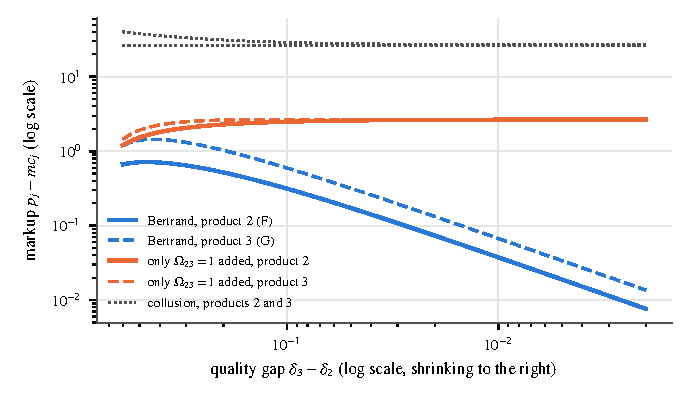
\includegraphics[width=0.74\textwidth]{figures/ch06/bresnahan_limit.pdf}
\caption{Markups of products 2 and 3 as their quality gap shrinks, in the seven-product design of
\cref{fig:06-bres-fig2}. Under Bertrand competition between their owners (blue) both markups fall in proportion to
the gap, as in \cref{prop:06-bertrand-limit}(a). If the Bertrand ownership matrix is changed only by letting
products 2 and 3 cooperate, $\Omega_{23} = 1$ (orange), the markups converge to a common positive value near 2.67,
as in part (b). Under full collusion (gray) they converge to about
26.7, the value given by \cref{eq:06-bres-mC}. Both axes are logarithmic. Computed with
\texttt{bresnahan\_fig2\_sim.py}.}
\label{fig:06-bres-limit}
\end{figure}

\subsubsection{The intuition and Bresnahan's Figure 2}\label{sec:06-bres-intuition}

Bresnahan states the intuition in two sentences \citep[p.~458]{Bresnahan1987}. If firms compete in prices, price is
near marginal cost for the products that have a close substitute sold by a competitor. If firms collude, the markup
on one firm's product hardly depends on whether its close substitutes are sold by competitors or by the firm itself.
\Cref{prop:06-bertrand-limit,prop:06-bres-collusion} make both sentences precise. Bresnahan adds a general point.
Conduct hypotheses differ in the comparative statics of price and quantity with respect to demand elasticities. So
conduct can be discerned even when marginal costs are unobserved, the same logic as the rotation argument of
\cref{ch:conduct}.

His Figure 2 illustrates the point with seven products in quality space and two firms, labelled G and F. We
recreate its design by solving the model. Products 2 and 3 are almost identical and belong to different firms.
Products 5, 6 and 7, at the top, all belong to G. \Cref{fig:06-bres-fig2} plots marginal cost and equilibrium prices
against quality under both conduct hypotheses, and \cref{fig:06-bres-fig2-orig} shows the original.\footnote{The
text of \citet[p.~466]{Bresnahan1987} describes the example differently from the figure. It says that ``Firm One
sells products 2, 4, and 5'' and that ``Firm Two sells product 3''. The prices of products 1 and 6 are held fixed,
because a third firm sells them. The figure labels the owners of products 1 to 7 as G, F, G, F, G, G, G. Our
recreation follows the figure. The economics is the same under both descriptions, because products 2 and 3 are
close neighbors owned by different firms.}

\begin{figure}[htbp]
\centering
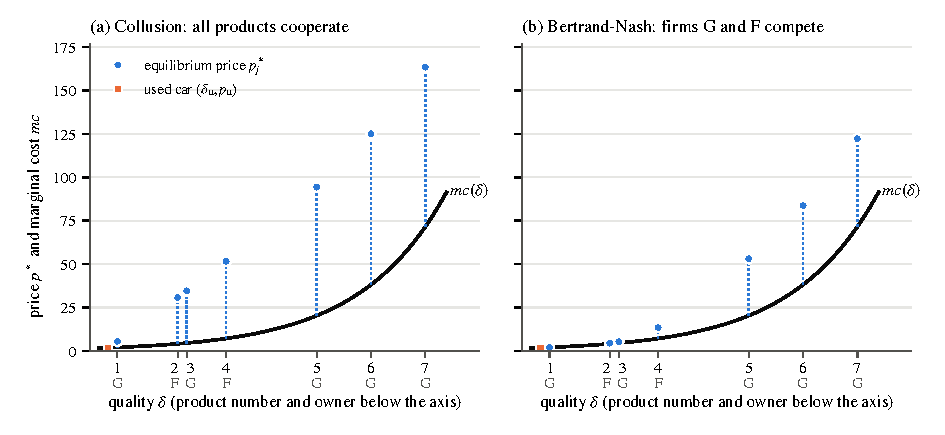
\includegraphics[width=\textwidth]{figures/ch06/bresnahan_fig2_sim.pdf}
\caption{Model-generated recreation of the design of \citet{Bresnahan1987}, Figure 2. Seven products with qualities
$\delta = (1, 2, 2.15, 2.8, 4.3, 5.2, 6.1)$ and owners G, F, G, F, G, G, G. Tastes are uniform with $\kappa = 1$ and
$\bar v = 48.3$. Marginal cost is $mc(\delta) = e^{0.7\delta}$, which is Bresnahan's $\psi e^{\delta}$ after a
rescaling of quality units. The used car has $\delta_{\mathrm u} = 0.85$ and $p_{\mathrm u} = mc(\delta_{\mathrm u})$.
Dots are equilibrium prices, and dotted segments are markups. Panel (a) solves \eqref{eq:06-bres-linear} with
$\Omega = \Omega^{\mathrm C}$ and panel (b) with the ownership matrix. Computed with \texttt{bresnahan\_fig2\_sim.py}.
The recreation copies the ownership labels of the original figure. Its markups need not match the original, which
Bresnahan drew as a sketch.}
\label{fig:06-bres-fig2}
\end{figure}

\begin{figure}[htbp]
\centering
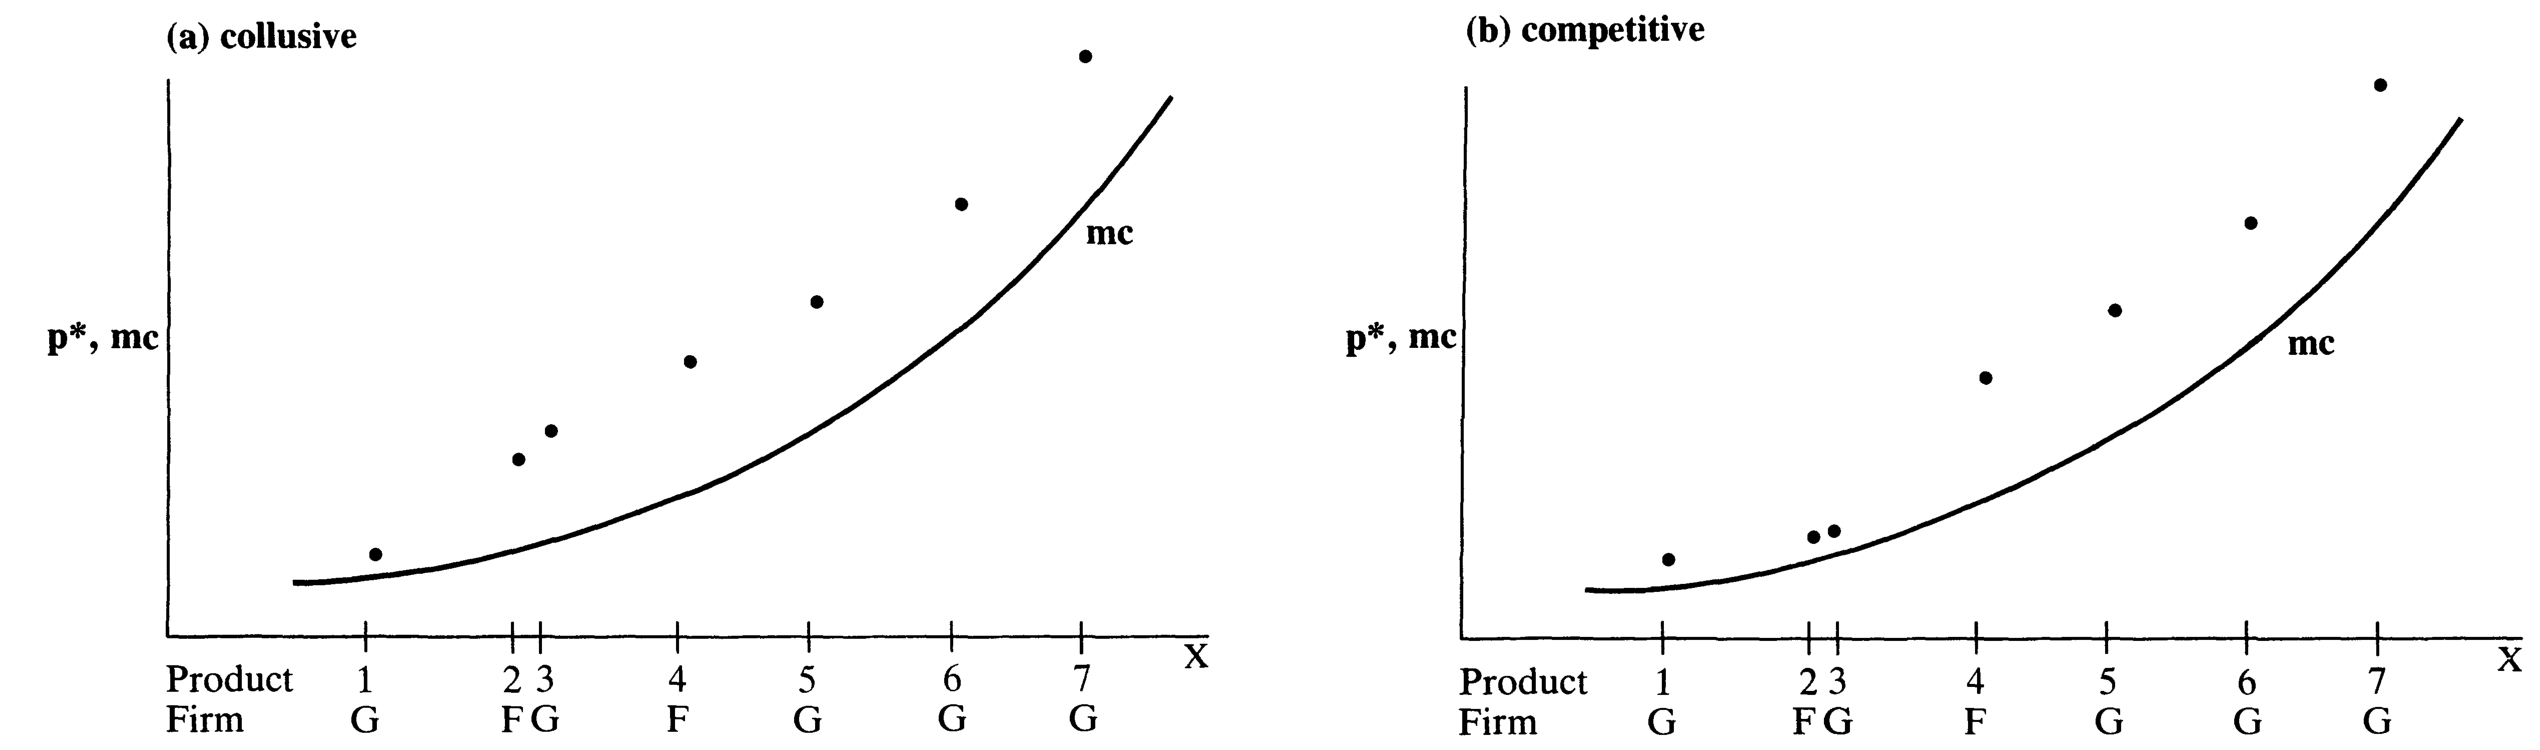
\includegraphics[width=\textwidth]{figures/ch06/bresnahan1987_fig2_orig.png}
\caption{Bresnahan's original illustration. Panel (a) shows collusive prices and panel (b) competitive prices, with
the marginal cost curve and the owner of each product below the quality axis. Source: \citet{Bresnahan1987},
Figure 2.}
\label{fig:06-bres-fig2-orig}
\end{figure}

The recreation shows three patterns. First, products 2 and 3 have markups of 26.65 and 30.05 under collusion and of
only 0.43 and 0.83 under Bertrand competition, so they sit on the cost curve in panel (b). Their rivalry is
fierce because they are close substitutes owned by different firms. Second, products 5, 6 and 7 keep between 44 and
55 percent of their collusive markups under Bertrand competition. They are distant from rivals and owned by one firm.
By \cref{rem:06-bres-topblock}, the price increments $p_6 - p_5$ and $p_7 - p_6$ and the quantities of products 6
and 7 are identical in the two panels. All three markups fall by the same amount, 41.28. Product 5 sells more under
Bertrand competition (7.61 against 5.50), because its lower cutoff falls when product 4 competes. Third, product 4,
owned by F and wedged between two G products at moderate distances, keeps 14 percent of its collusive markup. Most
of its Bertrand markup comes from the large markup of its upper neighbor, product 5, because prices are strategic
complements.

The recreation departs from Bresnahan's sketch in one visible respect. In his panel (b), products 4 to 7 keep nearly
all of their collusive markups. He writes that ``Products 4 and 5 change much less when the solution concept
changes'' \citep[p.~467]{Bresnahan1987}. In the solved model, product 4 keeps only 14 percent of its markup and
products 5 to 7 keep about half. Product 4 faces rival neighbors on both sides. Products 6 and 7 lose the same dollar
amount of markup as product 5, the lowest member of the top block (\cref{rem:06-bres-topblock}). Bresnahan's figure
is a sketch, and the robust contrast is the collapse of the markups of products 2 and 3.

The figure shows where the data can discriminate between the hypotheses. Regions of the quality ladder crowded with
products of different firms look very different under the two hypotheses. Regions with few firms change much less,
because market power is substantial even under competition. Bresnahan likens the large-car end of the mid-1950s
market, where GM produced most cars, to the region around products 4 and 5 of his example. He likens the
smaller-car segments to the region around products 1 and 2. There Ford, Chrysler, GM and, to a lesser extent, AMC
and the fringe were all present \citep[p.~467]{Bresnahan1987}. Bresnahan therefore expects the method to have statistical power in this industry. He also notes that the
method would be less revealing if every producer had a full product line \citep[p.~467]{Bresnahan1987}.
\Cref{rem:06-bres-power} makes this precise.

An earlier study supports this reading of the figure. \citet[pp.~1021--1022]{Bresnahan1989} summarizes
\citet{Bresnahan1981}, which fits the same vertical demand system to cross-sections of the 1977 and 1978 model
years. Its demand equation is the interior equation of \eqref{eq:06-bres-demand} (eq.~7 of the survey). Quality is
a hedonic function of length, weight, horsepower and other characteristics (eq.~8). The supply side is
\eqref{eq:06-bres-foc} under Bertrand conduct. Same-owner dummies on the two neighbors of each model play the role
of $\Omega_{j,j+1}$ and $\Omega_{j,j-1}$ (eq.~6$''$). The study reports two related findings. The large
price-cost margins appear on the larger vehicles, and the larger vehicles are much farther apart in quality space.
Products 5 to 7 of \cref{fig:06-bres-fig2} show the same pattern. They have no close rival, and they keep about
half of their collusive markups under Bertrand competition, while products 2 and 3 keep almost nothing. Bresnahan
adds that the finding confirms the view of industry observers based on accounting profits (footnote~13 of the
survey).

\subsection{Econometric specification and estimation}\label{sec:06-bres-estimation}

\casehead{Quality as an index of characteristics}
Quality is not observed. Bresnahan proxies it with a function of the physical characteristics (his eq.~22):
\begin{equation}\label{eq:06-bres-quality}
  \delta(x_j) = \sqrt{\beta_0 + x_j\beta},
\end{equation}
where $\beta_0$ and the vector $\beta$ are parameters. The interpretation comes from the hedonic model of
\citet{Rosen1974}, developed in \cref{sec:06-hedonic}. Consumers have preferences over characteristics, and firms
produce bundles of characteristics at costs that depend on them. The index is read as the expansion path of
efficient, cost-minimizing bundles. Each quality level is produced with the cheapest combination of characteristics
that delivers it. For this reason $\beta$ mixes information about tastes and technology, and its interpretation is
``clouded'' \citep[p.~467]{Bresnahan1987}. The square-root form is an arbitrary choice.

\casehead{Computing the model's predictions}
The parameters are $\theta = (\beta_0, \beta, \psi, \delta_{\mathrm u}, \bar v, \kappa)$, and the conduct hypothesis
fixes $\Omega$. For each trial value of $\theta$ the predictions are computed in three steps.
\begin{enumerate}
\item Compute every model's quality $\delta_j$ from \eqref{eq:06-bres-quality}.
\item Rank the models by quality, which determines who neighbors whom.
\item Solve the demand system \eqref{eq:06-bres-demand} and the first-order conditions \eqref{eq:06-bres-foc}
jointly for the predicted prices $p^*_j(\theta,\Omega)$ and quantities $q^*_j(\theta,\Omega)$, which amounts to the
linear system \eqref{eq:06-bres-linear}.
\end{enumerate}
The predictions depend only on parameters and on the exogenous characteristics. The used-car parameters are tied
together by \cref{ass:06-bres}(v), because the demand for the lowest-quality model \eqref{eq:06-bres-demand} is
overparameterized in $(\delta_{\mathrm u}, p_{\mathrm u})$. Bresnahan imposed $p_{\mathrm u} = mc(\delta_{\mathrm u})$
after initial experimentation showed the two were not easily distinguishable (p.~468).

\casehead{Errors and likelihood}
Observed prices and quantities equal the predictions plus additive, independent normal errors. Price errors have
variance $\sigma_p^2$. The error on aggregated quantity $m$ has variance $k_m\sigma_q^2$, from
\cref{sec:06-bres-data}, and price and quantity errors are independent. The likelihood is (his eq.~24)
\begin{equation}\label{eq:06-bres-lik}
  L(\theta,\sigma_p^2,\sigma_q^2)
  = \prod_{j=1}^{N_p}\frac{1}{\sqrt{2\pi\sigma_p^2}}\exp\Bigl[-\frac{(p_j - p_j^*)^2}{2\sigma_p^2}\Bigr]
    \prod_{m=1}^{N_q}\frac{1}{\sqrt{2\pi k_m\sigma_q^2}}
    \exp\Bigl[-\frac{\bigl(q_m - \sum_{j\in\mathcal I_m}q_j^*\bigr)^2}{2k_m\sigma_q^2}\Bigr],
\end{equation}
where $N_p$ and $N_q$ are the numbers of price and quantity observations and the predictions depend on
$(\theta,\Omega)$. The variances can be concentrated out. The log-likelihood is
\begin{equation*}
  \ln L = -\frac{N_p}{2}\ln(2\pi\sigma_p^2) - \frac{1}{2\sigma_p^2}\sum_{j}(p_j - p_j^*)^2
          - \frac{1}{2}\sum_m \ln(2\pi k_m\sigma_q^2) - \frac{1}{2\sigma_q^2}\sum_m \frac{(q_m - \sum_{j\in\mathcal I_m}q_j^*)^2}{k_m}.
\end{equation*}
Setting the derivative with respect to $\sigma_p^2$ to zero gives
$-\frac{N_p}{2\sigma_p^2} + \frac{1}{2\sigma_p^4}\sum_j (p_j - p_j^*)^2 = 0$, and similarly for $\sigma_q^2$. Hence
\begin{equation*}
  \hat\sigma_p^2(\theta) = \frac{1}{N_p}\sum_{j=1}^{N_p}(p_j - p_j^*)^2,
  \qquad
  \hat\sigma_q^2(\theta) = \frac{1}{N_q}\sum_{m=1}^{N_q}\frac{\bigl(q_m - \sum_{j\in\mathcal I_m}q_j^*\bigr)^2}{k_m}.
\end{equation*}
Substituting back gives the concentrated log-likelihood
\begin{equation}\label{eq:06-bres-conclik}
  \ell^c(\theta) = -\frac{N_p}{2}\ln\hat\sigma_p^2(\theta) - \frac{N_q}{2}\ln\hat\sigma_q^2(\theta)
  - \frac{1}{2}\sum_{m}\ln k_m - \frac{N_p + N_q}{2}\bigl(1 + \ln 2\pi\bigr).
\end{equation}
Maximum likelihood therefore chooses $\theta$ to minimize $N_p\ln\hat\sigma_p^2(\theta) + N_q\ln\hat\sigma_q^2(\theta)$.
Equivalently, it minimizes the product $(\hat\sigma_p^2)^{N_p}(\hat\sigma_q^2)^{N_q}$ of the mean squared price error
and the weighted mean squared quantity error. It is a form of nonlinear least squares for a system of two equations. All
estimation was done by numerical maximization.

\begin{remark}[A reduced-form error structure]\label{rem:06-bres-reducedform}
The errors in \eqref{eq:06-bres-lik} are appended to the equilibrium predictions. They are not structural demand or
cost shocks. Bresnahan calls this ``fully a reduced-form error structure'' (p.~469). It avoids the usual
endogeneity problem, because price never appears as a regressor and the predictions depend only on exogenous
characteristics. The cost of this choice is that the errors have no economic interpretation. A cost shock to one model would move
its neighbors' prices through the first-order conditions, which additive independent errors cannot capture.
\citet[p.~843]{BerryLevinsohnPakes1995} note that Bresnahan ``allows prices to be correlated with a linear
disturbance in an equilibrium pricing equation''. They add that he ``does not explicitly model the correlation
between prices and unobserved characteristics.'' Modelling an unobserved product characteristic $\xi_j$ and inverting market shares is
the response of \citet{Berry1994} and \citet{BerryLevinsohnPakes1995} (\cref{ch:logit,ch:blp}).
\end{remark}

\casehead{An irregular likelihood}
The likelihood is not continuous in the parameters. Predicted prices are continuous, but predicted quantities jump
at values of $\beta$ where two models, or a model and the used car, tie in quality. At such points the ranking
changes, and so does the set of neighbors. A discontinuous function cannot be concave, and the standard regularity
conditions for nonlinear regression fail. Bresnahan argues that ties are unlikely at the true parameter value, so
that limiting inference should go through (his footnote~9). He also reports that no local maxima caused trouble and
that the points of discontinuity were typically local minima, since they imply extreme predicted quantities
(footnote~10). Asymptotic normality of the estimators and of the test statistics remains unproven, as Appendix~B
acknowledges.

\casehead{Two further specifications}
Two more models serve as alternatives in the tests. The first is the log-linear hedonic model of
\citet{CowlingCubbin1971}, estimated on the British car market. Predicted prices and quantities follow a recursive
structure (his eqs.~25--26):
\begin{equation}\label{eq:06-bres-hedonic}
  p_j^* = \exp\bigl(a_0 + x_j a\bigr),
  \qquad
  q_j^* = \exp\bigl(l_0 + l_1(p_j - p_j^*)\bigr),
\end{equation}
where we write $a_0$, $a$, $l_0$ and $l_1$ for Bresnahan's $\alpha_0$, $\alpha_j$, $\lambda_0$ and $\lambda_1$. The
price equation adds GM and Ford dummies, following authors who use firm dummies as a proxy for market power. The
model has the same error and aggregation structure as the oligopoly models. \citet{Rosen1974} interprets a hedonic
price function as the equilibrium of a perfectly competitive, continuously differentiated market. The hedonic model,
``or something like it'', should hold if list prices were set in some nonmaximizing way (p.~470). It differs
radically from the oligopoly models. The second alternative, called ``Products'', is the opposite. It follows the
oligopoly model exactly but treats every model as if a separate firm made it, so $\Omega = I$. Neither is an
appealing story of the industry. Both are useful as tests, because an oligopoly model that survives against them
is more credible.

\subsection{Testing non-nested conduct hypotheses}\label{sec:06-bres-cox}

Collusion and Bertrand competition are non-nested hypotheses. They impose different matrices $\Omega$, and no
restriction on the parameters turns one model into the other. The hedonic model is a different family altogether.
A classical likelihood ratio test, which compares a model with a restricted version of itself, does not apply.
Bresnahan uses the non-nested test of \citet{Cox1961} in the regression form of \citet{PesaranDeaton1978}
\citep[p.~470]{Bresnahan1987}.

\casehead{The Cox statistic}
Let $H_0$ and $H_1$ be two parametric models for the same data, with maximized log-likelihoods $L_0$ and $L_1$. The
\emph{Cox statistic} for testing $H_0$ against $H_1$ is the observed log-likelihood ratio minus an estimate of its
expectation under $H_0$,
\begin{equation}\label{eq:06-bres-coxstat}
  T_0 = (L_0 - L_1) - \hat\E_0\bigl[L_0 - L_1\bigr].
\end{equation}
The expectation is evaluated at the estimate of $\theta_0$. It replaces the parameters of $H_1$ by their
\emph{pseudo-true values}, the probability limit of the $H_1$ estimator when the data come from $H_0$. Under $H_0$ the
standardized statistic is asymptotically standard normal. A significantly negative $T_0$ means that $H_1$ fits better
than it should if $H_0$ were true, which is evidence against $H_0$ in the direction of $H_1$. A significantly positive
$T_0$ means that $H_1$ fits worse than $H_0$ predicts. The test is two-tailed, so this also rejects $H_0$, whose
likelihood is ``too large'' relative to $H_1$. The test is not symmetric. Testing $H_1$ against $H_0$ is a different
test, so both models can be rejected, or neither. The next proposition gives the statistic for regression models.

\begin{proposition}[Cox statistic for non-nested regressions]\label{prop:06-bres-cox}
Let $y \in \R^N$, $H_0: y = f_0(\theta_0) + u$ and $H_1: y = f_1(\theta_1) + w$, with $u \sim N(0,\sigma_0^2 I_N)$ under
$H_0$, smooth mean functions, and parameter vectors of fixed dimension. Let $s_0^2$ and $s_1^2$ be the maximum
likelihood residual variances under the two models. Fit $H_1$ to the fitted values of $H_0$: let
$\hat\theta_{10}$ minimize $\|f_0(\hat\theta_0) - f_1(\theta_1)\|^2$, let $\hat d = f_0(\hat\theta_0) - f_1(\hat\theta_{10})$,
and define
\begin{equation*}
  \phi^2 = \frac{1}{N}\|\hat d\|^2,
  \qquad s_{10}^2 = s_0^2 + \phi^2,
  \qquad \tilde\phi = \frac{1}{N}\hat d^\top M_0\hat d,
\end{equation*}
where $M_0 = I_N - F_0(F_0^\top F_0)^{-1}F_0^\top$ and $F_0 = \frac{\partial f_0(\hat\theta_0)}{\partial\theta_0^\top}$. Then
\begin{equation*}
  T_0 = \frac{N}{2}\ln\frac{s_1^2}{s_{10}^2}.
\end{equation*}
If $H_0$ is true, $H_1$ does not contain the true mean function, and standard regularity conditions hold, then
\begin{equation*}
  \frac{T_0}{\sqrt{V_0}} \xrightarrow{d} N(0,1),
  \qquad
  V_0 = \frac{N\tilde\phi\, s_0^2}{s_{10}^4}.
\end{equation*}
\end{proposition}

\begin{proof}[Proof sketch]
The concentrated log-likelihood of a normal regression is $-\frac{N}{2}\ln s^2$ plus a constant common to both
models. Hence
\begin{equation*}
  L_0 - L_1 = \frac{N}{2}\ln\frac{s_1^2}{s_0^2}.
\end{equation*}
Under $H_0$, $s_1^2$ converges to $\sigma_0^2 + \phi_*^2$, where $\phi_*^2$ is the limit of $\phi^2$, the part of the
$H_0$ mean that $H_1$ cannot fit. The estimated expectation of $L_0 - L_1$ is therefore
$\frac{N}{2}\ln\frac{s_{10}^2}{s_0^2}$, and subtracting it gives $T_0$.

For the distribution we expand to first order around the true $\theta_0$ and the pseudo-true value
$\theta_{10}^*$. Write $f_0 = f_0(\theta_0)$ and $d = f_0 - f_1(\theta_{10}^*)$. Let $F_1$ be the gradient of $f_1$ at
$\theta_{10}^*$, define $M_1$ from $F_1$ as $M_0$ is defined from $F_0$, and let $P_k = I_N - M_k$ be the projection
onto the columns of $F_k$. The first-order condition
defining $\theta_{10}^*$ is $F_1^\top d = 0$, so $M_1d = d$. Four steps follow.
\begin{enumerate}
\item Fitting $H_1$ to $y = f_0 + u$ leaves residuals $M_1(d + u)$ to first order. Hence
$Ns_1^2 \approx \|d\|^2 + 2d^\top u + u^\top M_1 u$.
\item Fitting $H_0$ leaves residuals $M_0u$, so $Ns_0^2 \approx u^\top M_0 u$.
\item The fitted values of $H_0$ are $f_0 + P_0u$ to first order. Fitting $H_1$ to them, as in step 1, gives
$N\phi^2 \approx \|d\|^2 + 2d^\top P_0u + u^\top P_0M_1P_0u$.
\item Subtracting, $N(s_1^2 - s_{10}^2) \approx 2d^\top M_0 u + R$, where $R$ collects quadratic forms in $u$ on spaces of
fixed dimension and is bounded in probability. The term $d^\top M_0u$ is of order $\sqrt N$ because
$\|d\|^2$ grows like $N$.
\end{enumerate}
Since $\ln\frac{s_1^2}{s_{10}^2} \approx \frac{s_1^2 - s_{10}^2}{s_{10}^2}$, the statistic satisfies
\begin{equation*}
  T_0 \approx \frac{d^\top M_0u}{\sigma_0^2 + \phi_*^2},
  \qquad
  \Var_0\bigl(d^\top M_0 u\bigr) = \sigma_0^2\, d^\top M_0 d .
\end{equation*}
The leading term is normal with mean zero and variance $\frac{\sigma_0^2\, d^\top M_0 d}{(\sigma_0^2 + \phi_*^2)^2}$. Its
plug-in estimate is $V_0$, since $N\tilde\phi$ estimates $d^\top M_0d$. \citet{Pesaran1974} and
\citet{PesaranDeaton1978} give the regularity conditions and the multivariate version.
\end{proof}

The proof explains the two auxiliary regressions in Bresnahan's Appendix B. The first fits $H_1$ to the fitted
values of $H_0$, which he calls the ``phony-data regression''. Its residual variance $\phi^2$ measures how far $H_1$
is from $H_0$. The second regresses the phony-data residuals on the derivatives of $H_0$'s predictions. Its
residual variance $\tilde\phi$ removes the part of the distance that a small change in $\theta_0$ could absorb.
The intuition of the test is simple: $H_0$ is rejected if $H_1$ explains a significant part of $H_0$'s
residuals \citep[p.~471]{Bresnahan1987}.

\casehead{Bresnahan's formulas}
Bresnahan's models have two equations with independent errors, and the quantity equation is weighted by
$\frac{1}{k_m}$. The concentrated log-likelihood \eqref{eq:06-bres-conclik} has the same weights under every model,
so the terms in $k_m$ cancel from all likelihood ratios. The contributions of the two equations add. Let $s^2_{jp}$
and $s^2_{jq}$ be the estimated price and quantity error variances under $H_j$, for $j = 0, 1$ (his eqs.~B.1--B.2).
The phony-data regression fits $H_1$ to the predictions of $H_0$ and yields variances $\phi^2_p$ and $\phi^2_q$. Then
(his eqs.~B.3--B.5)\footnote{Equation (B.4) is printed as $s^2_{10q} \equiv s^2_{0p} + \phi^2_q$. The subscript $0p$ is
a misprint for $0q$, by analogy with (B.3) and with \cref{prop:06-bres-cox}.}
\begin{equation}\label{eq:06-bres-T0}
  s^2_{10p} = s^2_{0p} + \phi^2_p,
  \qquad
  s^2_{10q} = s^2_{0q} + \phi^2_q,
  \qquad
  T_0 = \frac{N_p}{2}\ln\frac{s^2_{1p}}{s^2_{10p}} + \frac{N_q}{2}\ln\frac{s^2_{1q}}{s^2_{10q}} .
\end{equation}
The second regression takes the residuals of the phony-data regression and regresses them linearly on the
derivatives of the $H_0$ predictions with respect to the $H_0$ parameters. Its residual variances are
$\tilde\phi_p$ and $\tilde\phi_q$, which Bresnahan writes as $\phi p$ and $\phi q$. They are variances in their own
right. They are not the square roots of $\phi^2_p$ and $\phi^2_q$. The asymptotic variance of $T_0$ is (his eq.~B.6)
\begin{equation}\label{eq:06-bres-V0}
  V_0(T_0) = N_p\tilde\phi_p\,\frac{s^2_{0p}}{s^4_{10p}} + N_q\tilde\phi_q\,\frac{s^2_{0q}}{s^4_{10q}},
\end{equation}
and the test statistic is $\frac{T_0}{\sqrt{V_0(T_0)}}$.\footnote{Appendix B prints the statistic as the ratio of $T_0$ to $V(T_0)$, without a square root. The text
(p.~470) divides the deviation of the likelihood ratio from its mean ``by its standard deviation''.
\Cref{prop:06-bres-cox} confirms that the square root is required for an asymptotically standard normal statistic. We
read the printed ratio as shorthand.} Each term of \eqref{eq:06-bres-T0} and \eqref{eq:06-bres-V0} is the
single-equation formula of \cref{prop:06-bres-cox}. Bresnahan's footnote~11 notes that the Pesaran-Deaton formulas were
altered slightly to account for the aggregation of quantities.

\begin{table}[htbp]
\centering
\caption{Cox test statistics for each maintained hypothesis against each alternative, 1954--1956}
\label{tab:06-bres-cox}
\small
\begin{tabular}{@{}lrrrr@{}}
\toprule
 & \multicolumn{4}{c}{Alternative hypothesis $H_1$} \\
\cmidrule(l){2-5}
Maintained hypothesis $H_0$ & Collusion & Nash-Competition & ``Products'' & Hedonic \\
\midrule
\multicolumn{5}{@{}l}{\textit{(a) 1954}} \\
Collusion        & $\cdot$     & 0.8951      & 0.9464      & $-1.934$ \\
Nash-Competition & $-2.325^{*}$ & $\cdot$    & $-0.8878$   & $-2.819^{*}$ \\
``Products''     & $-3.978^{*}$ & $3.029^{*}$ & $\cdot$    & $-1.604$ \\
Hedonic          & $-12.37^{*}$ & $-10.94^{*}$ & $-13.02^{*}$ & $\cdot$ \\
\addlinespace
\multicolumn{5}{@{}l}{\textit{(b) 1955}} \\
Collusion        & $\cdot$     & $-10.36^{*}$ & $-9.884^{*}$ & $-13.36^{*}$ \\
Nash-Competition & $-1.594$    & $\cdot$      & 1.260        & 0.6341 \\
``Products''     & $-0.7598$   & $-4.379^{*}$ & $\cdot$      & $-1.527$ \\
Hedonic          & $-3.353^{*}$ & $-8.221^{*}$ & $-5.950^{*}$ & $\cdot$ \\
\addlinespace
\multicolumn{5}{@{}l}{\textit{(c) 1956}} \\
Collusion        & $\cdot$     & 1.227        & 0.8263       & 1.629 \\
Nash-Competition & $-2.426^{*}$ & $\cdot$     & $-4.586^{*}$ & 0.8314 \\
``Products''     & $-3.153^{*}$ & 0.9951      & $\cdot$      & $4.731^{*}$ \\
Hedonic          & $-5.437^{*}$ & $-9.671^{*}$ & $-11.58^{*}$ & $\cdot$ \\
\bottomrule
\end{tabular}

\smallskip
\begin{minipage}{0.92\textwidth}
\footnotesize
\emph{Notes:} Reproduced from \citet[Table III, p.~471]{Bresnahan1987}. Each entry is the standardized Cox
statistic $\frac{T_0}{\sqrt{V_0}}$ for testing the row model against the column model, asymptotically standard
normal under the row model. A dot marks the diagonal. Asterisks are ours and mark rejection at the 5 percent level
in a two-tailed test, $\bigl|\frac{T_0}{\sqrt{V_0}}\bigr| > 1.96$. Negative values indicate that the alternative fits better than the maintained
model predicts. ``Products'' treats every model as a separate firm ($\Omega = I$). The hedonic model is
\eqref{eq:06-bres-hedonic}.
\end{minipage}
\end{table}

\casehead{Results}
\Cref{tab:06-bres-cox} reproduces the test results. In 1954 the hedonic model is rejected against every other
model. ``Products'' is rejected against both oligopoly models but not against the hedonic model.
Nash-Competition is rejected against Collusion ($-2.325$) and against the hedonic model ($-2.819$). Collusion is the
only model that escapes rejection against every alternative. Its statistic against the hedonic model, $-1.934$, is
close to the 5 percent cutoff of 1.96 but below it in absolute value. The 1956 results resemble those of 1954. Collusion is not
rejected against any alternative, and every other model is rejected at least once. Nash-Competition, for example,
is rejected against Collusion ($-2.426$) and against ``Products'' ($-4.586$).

The 1955 results are reversed. Collusion is rejected against all three alternatives, with statistics of $-10.36$,
$-9.884$ and $-13.36$. Nash-Competition is rejected against none. The other models are rejected as in the
surrounding years. ``Products'' is rejected against Nash-Competition, and the hedonic model against everything.
Some rejections have positive signs, as for ``Products'' against Nash-Competition in 1954 ($3.029$) and against the
hedonic model in 1956 ($4.731$). These reject because the likelihood of ``Products'' is too large relative to the
alternative, a possibility Bresnahan's footnote~12 points out for the two-tailed test.

Bresnahan stresses that the test results and the output expansion are independent evidence. Each year is estimated
separately, and no cross-year restriction, for example on the location of the demand curve, forces the competitive
model to be chosen in the high-quantity year. The coincidence of the reversal with the boom is therefore
informative \citep[p.~472]{Bresnahan1987}. The results are also robust to the two added specifications, which are
rejected throughout. The hedonic model is the cleanest of these rejections, since its likelihood is regular and the
caveat on asymptotic normality does not apply to it.

\subsection{Estimates}\label{sec:06-bres-estimates}

\begin{table}[t]
\centering
\caption{Parameter estimates under the maintained conduct hypotheses, 1954--1956}
\label{tab:06-bres-iv}
\small
\begin{tabular}{@{}lccc@{}}
\toprule
Parameter & 1954 (Collusion) & 1955 (Bertrand) & 1956 (Collusion) \\
\midrule
\multicolumn{4}{@{}l}{\textit{Quality index $\delta(x) = \sqrt{\beta_0 + x\beta}$}} \\
Constant $\beta_0$          & 47.91    & 48.28    & 50.87 \\
                            & (32.8)   & (43.2)   & (29.4) \\
Weight (thousands of lb)    & 0.3805   & 0.5946   & 0.5694 \\
                            & (0.332)  & (0.145)  & (0.374) \\
Length (thousands of in.)   & 0.1819   & 0.1461   & 0.1507 \\
                            & (0.128)  & (0.059)  & (0.146) \\
Horsepower (hundreds)       & 2.665    & 3.350    & 3.248 \\
                            & (0.692)  & (0.535)  & (0.620) \\
Cylinders                   & $-0.7387$ & $-0.9375$ & $-0.9639$ \\
                            & (0.205)  & (0.115)  & (0.186) \\
Hardtop dummy               & 0.9445   & 0.4531   & 0.4311 \\
                            & (0.379)  & (0.312)  & (0.401) \\
\addlinespace
\multicolumn{4}{@{}l}{\textit{Demand and supply}} \\
Marginal cost scale $\psi$  & 0.1753   & 0.1747   & 0.1880 \\
                            & (0.024)  & (0.020)  & (0.035) \\
Used-car quality $\delta_{\mathrm u}$ & 4.593 & 3.911 & 4.441 \\
                            & (1.49)   & (2.08)   & (1.46) \\
Upper endpoint $\bar v$     & $1.92\times10^{7}$ & $2.41\times10^{7}$ & $2.83\times10^{7}$ \\
                            & $(8.44\times10^{6})$ & $(9.21\times10^{6})$ & $(7.98\times10^{6})$ \\
Taste density $\kappa$      & 0.4108   & 0.4024   & 0.4075 \\
                            & (0.138)  & (0.184)  & (0.159) \\
\bottomrule
\end{tabular}

\smallskip
\begin{minipage}{0.86\textwidth}
\footnotesize
\emph{Notes:} Reproduced from \citet[Table IV, p.~472]{Bresnahan1987}. Asymptotic standard errors in parentheses.
Each column uses the conduct hypothesis not rejected in \cref{tab:06-bres-cox}. The mapping to Bresnahan's symbols
is: $\psi$ is his $\mu$, $\delta_{\mathrm u}$ is his $\gamma$, $\bar v$ is his $V_{\max}$, and $\kappa$ is his
$\delta$. The paper does not report the numbers of price and quantity observations.
\end{minipage}
\end{table}

\Cref{tab:06-bres-iv} reports the estimates under the specification that survives the tests in each year: Collusion
for 1954 and 1956 and Bertrand for 1955. The three columns are close. The marginal-cost scale is
0.1753, 0.1747 and 0.1880. The taste density is 0.4108, 0.4024 and 0.4075. The quality-index coefficients are close
in size and sign across years. The estimated primitives barely move, so the change in conduct alone captures the distinct
features of 1955.

\begin{table}[t]
\centering
\caption{Parameter estimates when one conduct hypothesis is imposed in every year}
\label{tab:06-bres-v}
\footnotesize
\setlength{\tabcolsep}{4pt}
\begin{tabular}{@{}lcccccc@{}}
\toprule
 & \multicolumn{3}{c}{(i) Collusive specification} & \multicolumn{3}{c}{(ii) Bertrand specification} \\
\cmidrule(lr){2-4}\cmidrule(l){5-7}
Parameter & 1954 & 1955 & 1956 & 1954 & 1955 & 1956 \\
\midrule
Constant $\beta_0$ & 47.91 & $-23.37$ & 50.87 & 31.64 & 48.28 & 33.23 \\
  & (32.8) & (24.5) & (29.4) & (29.9) & (43.2) & (17.8) \\
Weight & 0.3805 & 0.0103 & 0.5694 & 0.9311 & 0.5946 & $6.23\times10^{-3}$ \\
  & (0.332) & $(5.43\times10^{-2})$ & (0.374) & (0.210) & (0.145) & $(8.73\times10^{-4})$ \\
Length & 0.1819 & $-2.88\times10^{-3}$ & 0.1507 & 0.1474 & 0.1461 & 0.1605 \\
  & (0.128) & (0.102) & (0.146) & (0.038) & (0.059) & (0.149) \\
Horsepower & 2.665 & 0.1165 & 3.248 & 4.962 & 3.350 & $2.972\times10^{-2}$ \\
  & (0.692) & (0.106) & (0.620) & (0.676) & (0.535) & $(1.47\times10^{-2})$ \\
Cylinders & $-0.7387$ & $-1.309$ & $-0.9639$ & $-0.8846$ & $-0.9375$ & $-0.9078$ \\
  & (0.205) & (1.52) & (0.186) & (0.194) & (0.115) & (0.256) \\
Hardtop & 0.9445 & 1.468 & 0.4311 & $-0.2474$ & 0.4531 & 0.5282 \\
  & (0.379) & (1.08) & (0.401) & (0.464) & (0.312) & (0.249) \\
$\psi$ & 0.1753 & 1.344 & 0.1880 & 0.2518 & 0.1747 & 0.2902 \\
  & (0.024) & (0.151) & (0.035) & (0.074) & $(0.312)^{a}$ & $(0.249)^{a}$ \\
$\delta_{\mathrm u}$ & 4.593 & 1.604 & 4.441 & 6.352 & 3.911 & 1.204 \\
  & (1.49) & (4.83) & (1.46) & (3.54) & (2.08) & (3.19) \\
$\bar v$ & $1.92\times10^{7}$ & $1.46\times10^{8}$ & $2.83\times10^{7}$ & $9.81\times10^{5}$ & $2.41\times10^{7}$ & $1.03\times10^{6}$ \\
  & $(8.44\times10^{6})$ & $(6.74\times10^{6})$ & $(7.98\times10^{6})$ & $(8.78\times10^{6})$ & $(9.21\times10^{6})$ & $(8.90\times10^{6})$ \\
$\kappa$ & 0.4108 & $5.75\times10^{-2}$ & 0.4075 & 5.04 & 0.4024 & 7.334 \\
  & (0.138) & $(8.28\times10^{-2})$ & (0.159) & (1.21) & (0.184) & (2.46) \\
\bottomrule
\end{tabular}

\smallskip
\begin{minipage}{0.95\textwidth}
\footnotesize
\emph{Notes:} Reproduced from \citet[Tables V(i) and V(ii), pp.~473--474]{Bresnahan1987}. Asymptotic standard errors in
parentheses. Symbols as in \cref{tab:06-bres-iv}. $^{a}$~Printed as in the source. These two standard errors
duplicate the hardtop standard errors directly above them, (0.312) and (0.249). Table IV reports (0.020) for the
same 1955 estimate of $\psi$, so the printed values are probably typesetting errors. The paper also reports Table
V(iii) for the hedonic model and Table V(iv) for ``Products''.
\end{minipage}
\end{table}

\Cref{tab:06-bres-v} tells the opposite story. When one conduct hypothesis is imposed in all three years, the
parameters must explain 1955 by themselves, and they behave erratically. Under the collusive specification the 1955
column departs from its neighbors. The marginal-cost scale $\psi$ is an order of magnitude larger, 1.344 against
0.1753 and 0.1880. The taste density $\kappa$ is an order of magnitude smaller, 0.0575 against about 0.41. The upper
endpoint $\bar v$ jumps to $1.46\times10^{8}$, and length receives a negative coefficient. The parameters must absorb
the low prices and high output that collusive pricing cannot generate with stable primitives.

The Bertrand specification is ``similarly chaotic'' \citep[p.~473]{Bresnahan1987}. Now 1954 and 1956 are the odd
years. The 1954 column has the only negative hardtop coefficient estimated in any year under any specification. In 1956 the
weight and horsepower coefficients collapse toward zero, to $6.23\times10^{-3}$ and $2.972\times10^{-2}$. Relative to
the surrounding years, tastes in 1955 are spread ``at one tenth the density over ten times the range'' (p.~475).
The comparison is with the Bertrand estimates for 1954 and 1956, where $\kappa$ is 5.04 and 7.334 and $\bar v$ is near
$10^{6}$. The 1955 values, 0.4024 and $2.41\times10^{7}$, are those of \cref{tab:06-bres-iv}, since both tables estimate 1955
under Bertrand.
Bresnahan sums up the comparison in one sentence: ``It is change of behavioral assumption, not change of parameter
values, that provides a reasonable empirical explanation of 1955'' (p.~475).

The lesson is general. A misspecified conduct assumption does not disappear. It is absorbed into the estimated
primitives, which then become unstable across periods and implausible in level. Stability of demand and cost
parameters across periods is therefore informative about conduct. \Cref{tab:06-bres-iv} is built from the two panels
of \cref{tab:06-bres-v}, and only the combination left unrejected by the tests produces a consistent picture.

The magnitudes in \cref{tab:06-bres-iv} have sensible readings \citep[p.~475]{Bresnahan1987}. The quality-index
coefficients have the signs and sizes one expects from hedonic regressions. The negative cylinders coefficient is
familiar from that literature too. Econometrically, horsepower and cylinders are highly collinear. Economically,
the cylinders variable captures the fall in the cost of horsepower after the introduction of the V-8 engine.

The demand parameters describe very diverse tastes for quality. The eight million buyers of 1955 had tastes $v$
between $4.24\times10^{6}$ and $2.4\times10^{7}$. In Bresnahan's words, the distribution was ``20 million wide and 0.4
deep'', and 20 million times 0.4 gives the eight million buyers. Bresnahan cautions that this may be an artifact of
the constant density. The same numbers imply a potential market of $\kappa\bar v = 0.4024\times 2.41\times10^{7}
\approx 9.7$ million in 1955, of whom about 1.7 million (those with $v$ below $4.24\times10^{6}$) chose the used
car. The used-car quality $\delta_{\mathrm u}$ is around 4 in each year, while the lowest new-car quality is around
9. New and used cars are thus not close substitutes. The parameter $\psi$ only converts quality units into money in
the marginal-cost function.

Two further readings concern 1956. The 1955 purchases do not seem to have depressed 1956 demand. Both $\kappa$ and $\bar v$
are slightly larger in 1956 than in 1955, and the 1954 and 1956 demand parameters are very similar. The used-car
quality rises from 3.911 in 1955 to 4.441 in 1956 (it was 4.593 in 1954), which Bresnahan reads as considerable competition from the used-car
market in 1956. For comparison, the hedonic model's quantity equation gives price coefficients $l_1$ of $-3.742$
(0.640), $-1.312$ (0.787) and $-3.322$ (0.715) in 1954, 1955 and 1956 (Table V(iii)). The 1955 coefficient is the
smallest in absolute value and the least precise.

\subsection{Counterfactual, fit and residuals}\label{sec:06-bres-fit}

\casehead{Collusion in 1955 as a counterfactual}
The estimates allow a simple decomposition of the 1955 expansion into demand and conduct. Bresnahan computes the
equilibrium with the 1955 parameters, which were estimated under Bertrand, but with the collusive solution. The
counterfactual prices are about one-half of one percent above the average of 1954 and 1956. Predicted 1955 unit
sales are 7.1 million, 25.5 percent above the 1954 and 1956 average, instead of the actual 40.4 percent. The change
in conduct thus accounts for about 0.8 million cars, the difference between 7.9 and 7.1 million. Bresnahan compares
this with the largest residual in the demand system of \citet{Chow1960}, $+0.6$ million units, which falls in 1955.
The two magnitudes are comparable. A supply-side change of the size implied by the price war is thus of the same
order as the part of 1955 that demand models could not explain.

\begin{table}[htbp]
\centering
\caption{Fit of the four models and residuals of the Big Three, 1954--1956}
\label{tab:06-bres-fit}
\small
\begin{tabular}{@{}lcccccc@{}}
\toprule
\multicolumn{7}{@{}l}{\textit{(a) $R^2$ of the price ($p$) and quantity ($q$) equations (Table VI)}} \\
\addlinespace
 & \multicolumn{2}{c}{1954} & \multicolumn{2}{c}{1955} & \multicolumn{2}{c}{1956} \\
\cmidrule(lr){2-3}\cmidrule(lr){4-5}\cmidrule(l){6-7}
Model & $p$ & $q$ & $p$ & $q$ & $p$ & $q$ \\
\midrule
Collusion    & 0.94 & 0.62 & 0.92 & 0.58 & 0.96 & 0.61 \\
Bertrand     & 0.91 & 0.62 & 0.96 & 0.64 & 0.93 & 0.62 \\
``Products'' & 0.90 & 0.62 & 0.88 & 0.59 & 0.92 & 0.61 \\
Hedonic      & 0.89 & 0.71 & 0.88 & 0.73 & 0.88 & 0.71 \\
\midrule
\multicolumn{7}{@{}l}{\textit{(b) Average residual of each firm minus the average of all other firms (Table VII)}} \\
\addlinespace
 & \multicolumn{2}{c}{1954 (Collusion)} & \multicolumn{2}{c}{1955 (Bertrand)} & \multicolumn{2}{c}{1956 (Collusion)} \\
\cmidrule(lr){2-3}\cmidrule(lr){4-5}\cmidrule(l){6-7}
Firm & Price & Quantity & Price & Quantity & Price & Quantity \\
\midrule
GM       & 20.92    & $-99.6$ & 28.80   & $-82.86$ & 21.48    & $-68.73$ \\
Ford     & $-12.33$ & 60.2    & $-6.28$ & 22.97    & $-11.02$ & 19.06 \\
Chrysler & $-13.16$ & 96.89   & $-9.33$ & 64.47    & $-17.19$ & 11.94 \\
\bottomrule
\end{tabular}

\smallskip
\begin{minipage}{0.92\textwidth}
\footnotesize
\emph{Notes:} Panel (a) reproduces \citet[Table VI, p.~476]{Bresnahan1987}. Because of the heteroskedasticity, the quantity
$R^2$ is defined as a fraction of explained variance, $R^2_q = \frac{s^2_q - \hat\sigma^2_q}{s^2_q}$. Here $s^2_q$ is the
second raw moment of the quantity data, computed under the same heteroskedastic variance structure as the models. Panel (b) reproduces Table VII (p.~477), computed from the unrejected specification in each
year. Price residuals are in dollars and quantity residuals in cars. ``All other firms'' includes the other two
firms of the Big Three.
\end{minipage}
\end{table}

\casehead{Fit}
Panel (a) of \cref{tab:06-bres-fit} gives part of the intuition behind the tests. The reversal between Collusion and
Bertrand appears as a reversal in $R^2$. In the price equation the unrejected model fits better in every year: 0.94
against 0.91 in 1954, 0.96 against 0.92 in 1955, and 0.96 against 0.93 in 1956. In the quantity equation it fits
better in 1955 (0.64 against 0.58) and equally well in 1954 (0.62 each).\footnote{Bresnahan writes that ``in each
year, the model not rejected explains more variance in both equations'' (p.~477). In 1956, however, Table VI gives
a quantity $R^2$ of 0.61 for Collusion and 0.62 for Bertrand, so the statement holds strictly only for the price
equation.} The hedonic model fits quantities better in every year, with $R^2_q$ of 0.71 to 0.73, yet the oligopoly
model left unrejected in each year is not rejected against it. Bresnahan concludes that the price equation provides most of the power of the
tests. His footnote~14 gives two reasons to read these $R^2$ values with care. The oligopoly models have no constant
in the quantity equation, by \eqref{eq:06-bres-demand}. In the price equation, marginal cost explains much of the
cross-sectional variance, so the price $R^2$ would be high even if little of the markup were explained.

\casehead{Residuals by firm}
Panel (b) compares the average residuals of each of the Big Three with those of all other firms. Since ``all other
firms'' for Ford and Chrysler includes GM, the clearest message concerns GM. Its average price residual is 20.92,
28.80 and 21.48 dollars, and its average quantity residual is $-99.6$, $-82.86$ and $-68.73$ cars. Bresnahan
summarizes these as overpredicting GM prices by about \$30, out of the \$1,500 price of a typical car. He also
describes them as underpredicting GM sales by about 100 units, out of typical sales near 60,000.\footnote{The paper does not define the
sign of a residual. Bresnahan's wording matches residuals defined as predicted minus observed values. Under the more
common convention, observed minus predicted, the same numbers would mean that the models underpredict GM prices and
overpredict GM sales. The magnitudes are unaffected. Note also that the printed price residuals, \$21 to \$29, are
somewhat below the \$30 of the text.} The errors are small, but they suggest that GM had a cost or quality advantage.
Bresnahan therefore estimated two broader specifications for each oligopoly model. One adds a GM dummy to the quality
index. The other gives GM its own marginal-cost scale. Neither GM parameter is significant in any unrejected
specification, and no Cox test result is reversed. Either parameter does make the GM residuals much closer to zero.

\subsection{Robustness}\label{sec:06-bres-robust}

Besides the GM extensions, Bresnahan reports two generalizations aimed at the most obvious weaknesses of the model.

\casehead{Quality measured with error}
The tests depend on which products are neighbors. Small errors in the imputed qualities could change the ranking of
products, and with it the pattern of same-firm and rival neighbors. Robert Masson raised this concern (footnote~15).
Following \citet{Bresnahan1981}, the quality index is rewritten as observed with error,
\begin{equation}\label{eq:06-bres-qerror}
  \delta(x_j) = \sqrt{\beta_0 + x_j\beta} + \zeta_j,
\end{equation}
where we write $\zeta_j$ for Bresnahan's $\varepsilon_x$.\footnote{The printed formula on p.~478 reads
$\sqrt{\beta_0 + \varepsilon_j\beta_jZ_j} + \varepsilon_x$. The first $\varepsilon_j$ is a misprint for the summation sign.}
Since quality is unobserved, $\zeta_j$ must be integrated out of the likelihood. This changes the substitution
pattern. With $\Var(\zeta_j) = 0$, each product is a substitute for exactly two others. As the variance grows, the
probability of demand-side interaction with less similar products rises, which ``smears'' the demand equations and
reduces the importance of very similar products. Bresnahan does not know how to construct Cox tests for this
specification. Its likelihoods, however, still favor Bertrand in 1955 and Collusion in the other years.

\casehead{Durability}
The model treats cars as a flow good, a ``glaring shortcoming'' for a durable \citep[p.~478]{Bresnahan1987}.
Bresnahan adds the stock of similar used cars to both equations:
\begin{equation}\label{eq:06-bres-durable}
  p_j = p_j^*(\theta,\Omega) + \lambda_S \mathcal{S}_j + e^p_j,
  \qquad
  q_j = q_j^*(\theta,\Omega) + \theta_S \mathcal{S}_j + e^q_j,
\end{equation}
where we write $\lambda_S$ and $\theta_S$ for his $\lambda$ and $\theta$, and $e^p_j$ and $e^q_j$ for his error terms.
Here $\mathcal{S}_j$ is the stock of used cars ``like'' model $j$, meaning within ten percent of its weight, with used cars
depreciating at 15 percent per year. The construction is ad hoc. Both coefficients differ significantly from zero,
but the Cox test results of \cref{tab:06-bres-cox} are unaltered. The rerun covers only the collusive and Bertrand
specifications (footnote~16).

Bresnahan draws two conclusions from these checks. The highly structured oligopoly models do not tell all of the
story the data have to tell, as the significant durability terms show. The conclusions about conduct nonetheless
appear robust.

\subsection{Identification}\label{sec:06-bres-ident}

Bresnahan observes no costs, no instruments in the modern sense, and no variation in ownership. The data for each
year are a single cross-section of about 80 to 85 models. We now state what pins down each object.

Demand and cost are identified within a conduct hypothesis by functional form and by the cross-section of prices
and quantities. Prices equal marginal cost plus a markup. Marginal cost is a smooth function $\psi e^{\delta(x)}$ of
characteristics, while markups depend on quantities and on the gaps between neighbors. The cross-sectional variation
of prices with characteristics therefore separates the cost curve from the markups, given the functional forms.
Quantities pin down the density $\kappa$, which scales all demand derivatives in \eqref{eq:06-bres-deriv}.

The scale of quality is fixed by the cost function. In the pure vertical model, quality is identified only up to the
scale of tastes, as \cref{prop:06-vscale} shows. Here, multiplying all qualities by $c$ and dividing all tastes by $c$
leaves choices unchanged, but it changes $\psi e^{\delta}$ to $\psi e^{c\delta}$. The exponential cost function and
the square-root index thus fix the units of quality. This is identification by functional form, and it is one reason
the specification matters.

Conduct is identified by how markups vary across products with the distance to the nearest neighbor and with the
owner of that neighbor. By \cref{prop:06-bertrand-limit,prop:06-bres-collusion}, the two hypotheses make sharply
different predictions for products with close neighbors owned by rivals. Within a year, the cross-section supplies
many such configurations. This plays the role that rotations of demand play in the homogeneous-goods conduct
literature (\cref{ch:conduct}). There, conduct is identified by changes in the slope of demand that leave costs
unchanged. Here, the gaps between neighbors are the slopes, and they vary across products within a market. The next
remark states exactly which features of ownership matter.

\begin{remark}[When can the data tell conduct apart?]\label{rem:06-bres-power}
By \eqref{eq:06-bres-Amat}, the matrix $A(\Omega)$ depends on $\Omega$ only through the neighbor entries
$\Omega_{j,j+1}$. Two conduct hypotheses that agree on every neighbor pair imply identical equilibrium prices and
quantities, and no data can distinguish them. Collusion and Bertrand differ exactly at the neighbor pairs owned by
different firms. Suppose each of $F$ firms sold one contiguous block of the quality ladder. The two hypotheses would then
differ at only $F - 1$ pairs, and \cref{rem:06-bres-topblock} shows that the top block would keep its collusive
price increments under both.
Interleaved product lines, as in the small-car segment of the 1950s, create many pairs where the hypotheses differ.
In the design of \cref{fig:06-bres-fig2}, the hypotheses differ at the four pairs from $(1,2)$ to $(4,5)$ and agree at
$(5,6)$ and $(6,7)$.
\end{remark}

Three further points complete the argument. First, the conduct hypotheses are discrete, and each is estimated
separately. The test compares the fit of two fully specified reduced forms \eqref{eq:06-bres-eqm}. No
continuous conduct parameter is estimated. Second, the hedonic and ``Products'' alternatives check that the oligopoly models
are not chosen merely because the alternatives are poor. Third, no restriction links the years, so the selection of
Bertrand in 1955 is not forced by the output spike. The same feature means that each year's identification rests on
its own cross-section and functional forms.

\subsection{Limitations and critiques}\label{sec:06-bres-limits}

\casehead{Restrictive substitution}
Quality is one-dimensional, so each product substitutes only with its two neighbors. This is exactly what gives the
test its power, and it is also the most criticized feature of the model. \citet[p.~852]{BerryLevinsohnPakes1995}
note that cross-price elasticities in the vertical model are determined by market shares and the rank order of
prices alone, not by characteristics such as size or power. Their example is a ranking with a \$24,998 family
station wagon, a \$24,999 sports car and a \$25,000 station wagon. The vertical model guarantees that the two wagons
are not substitutes for each other, while the sports car substitutes for both. \citet{FeenstraLevinsohn1995} allow
multidimensional differentiation while keeping the rest of Bresnahan's framework. Bresnahan's own error-in-quality
extension softens the restriction in the same direction.

\casehead{Functional forms}
The uniform taste distribution, the square-root quality index and the exponential cost function are all arbitrary.
They identify the scale of quality and shape the markups. Bresnahan concedes that the wide, shallow taste
distribution may be an artifact of the constant density.

\casehead{Unobserved quality and exogenous characteristics}
The errors are added to the reduced form, so there is no unobserved product characteristic that consumers see and
the econometrician does not (\cref{rem:06-bres-reducedform}). Characteristics are treated as exogenous, a defect that
\citet[p.~245]{Berry1994} notes his own approach shares with Bresnahan's and with nearly all studies of
differentiated products. Product lines are predetermined, so the model says nothing about how conduct might affect
product choice.

\casehead{Likelihood-based testing}
The non-nested tests require a fully specified likelihood, including the distribution of the errors and a complete
supply model. \citet[p.~335]{Nevo2001} cites this as a reason to prefer other comparisons of conduct. The likelihood is
also irregular, and the asymptotic distribution of the test statistics is unproven. Only the rejection of the
hedonic model is statistically clean.

\casehead{Data and dynamics}
Prices are list prices, and quantities are production rather than sales, which misses fleet sales and end-of-year
bargains. The model is static, while cars are durable and buyers can time purchases. The durability check of
\cref{sec:06-bres-robust} is ad hoc, and its terms are significant. The study covers three years chosen because one of
them is anomalous. Finally, the power of the test depends on crowded regions with interleaved owners, so the method
does not transfer to industries where each firm owns a contiguous segment.

\subsection{Contribution}\label{sec:06-bres-contribution}

Bresnahan's paper set the template for testing conduct with differentiated products. It specifies demand and cost
explicitly, solves for equilibrium under each conduct hypothesis, and asks which equilibrium fits the data. Conduct
enters as a discrete hypothesis about which products cooperate, encoded in the matrix $\Omega$.
This representation is the one that merger simulation uses when it changes ownership (\cref{ch:mergers}), and it is
the object later conduct tests compare.

The paper also showed that the fine structure of a cross-section carries information about conduct, even without
cost data. Markups of close rivals collapse under competition, while prices within a region owned by one firm move
together and keep their differences. Its finding that conduct changed for one year made the temporary breakdown of collusion an empirical
object. And its comparison of \cref{tab:06-bres-iv,tab:06-bres-v} teaches a lesson that applies far beyond
automobiles: imposing the wrong conduct leaves unstable and implausible primitives behind.

Later work kept the logic and replaced the parts that critics found weakest. \citet{Berry1994} and
\citet{BerryLevinsohnPakes1995} added unobserved product characteristics and richer substitution patterns, with
instruments for price (\cref{ch:logit,ch:blp}). \citet{Nevo2001} compared the margins implied by alternative conduct
hypotheses with observed margins. \citet{GasmiLaffontVuong1992} applied non-nested tests to conduct in a soft-drink
market, and \citet{Vuong1989} developed the model-selection tests that much of this literature uses
(\cref{app:econometrics}). \citet{BerryHaile2014} formalize when alternative oligopoly models can be distinguished
with market-level data, building on the early intuitions of \citet{Bresnahan1981,Bresnahan1982}.

\section{The idiosyncratic shock: tastes for products versus tastes for characteristics}\label{sec:06-epsilon}

Bresnahan's test draws its power from a demand system without an idiosyncratic shock. Each car competes only with
its neighbors on the quality ladder, and the Bertrand markups of close rivals vanish (\cref{prop:06-bertrand-limit}).
The logit-type models of \cref{ch:logit,ch:blp} make the opposite modeling choice. This section compares the two
classes directly, and the next two sections study estimators for models without the shock.

Every random utility model in this chapter can be written in the form
\begin{equation}\label{eq:06-u-general}
  u_{ij} = \delta_j + \mu_{ij} + \epsilon_{ij},
\end{equation}
where $\delta_j$ is the mean utility of product $j$. The consumer-specific deviation $\mu_{ij}$ comes from
interactions between consumer tastes and product characteristics. The idiosyncratic shock $\epsilon_{ij}$ is
independent across products and consumers. The logit, the nested logit and the random coefficients logit of
\cref{ch:logit,ch:blp} contain the shock. The Hotelling, ideal-point and vertical models of \cref{sec:06-models} do
not. This section asks what the shock does to the economics of a model. The short answer is that with
$\epsilon_{ij}$ the product space can never be exhausted. Each new product arrives with a fresh draw of $\epsilon_{ij}$
for every consumer. These draws guarantee the product a positive market share and some market power, whatever its
characteristics. \citet[p.~34]{AckerbergEtAl2007} question the economic content of the shock. They write that the
$\epsilon_{ij}$ ``are added to the model largely for computational convenience'' and ``do not seem to match any omitted
causal demand determinant.'' They add that the shocks give every conceivable product a strictly positive expected share.
Every product then has a positive cross-price effect with every other product, so that ``competition is never completely
local.'' We make these statements precise, following \citet{BerryPakes2007}, and then describe what the shock
buys in estimation.\footnote{As stated in \cref{sec:06-ps-cs}, citations of \citet{BerryPakes2007} use the
pages, footnotes, equations and tables of the author manuscript of July 2, 2007.}

\subsection{Two specifications of the consumer-specific term}\label{sec:06-tp-pc}

\citet{BerryPakes2007} start from a general indirect utility $u_{ij} = U(X_j, V_i; \theta)$ (their eq.~1). Here $X_j$
is the vector of characteristics of product $j$, price included, $V_i$ is a vector of consumer tastes and $\theta$ is a
parameter vector. They split $X_j = (x_j, \xi_j)$ into characteristics the econometrician observes and an unobserved
characteristic $\xi_j$ that consumers and firms see. They split $V_i = (z_i, \nu_i)$ into attributes $z_i$ that a
micro data set might record and unobserved tastes $\nu_i$. Empirical models then impose additive separability (their
eq.~3),
\begin{equation}\label{eq:06-bp-additive}
  u_{ij} = f(X_j, z_i; \theta) + \mu_{ij},
\end{equation}
and an assumption on the distribution of $\mu_{ij}$ given $(X_j, z_i)$. Both classes of models discussed below let
$\mu_{ij}$ contain linear interactions $\sum_k \nu_{ik} X_{jk}$, so each consumer has her own marginal utility for each
characteristic. The two classes differ in one respect only.

\begin{definition}[Tastes for products and pure characteristics]\label{def:06-tp-pc}
A random utility model has \emph{tastes for products} if
\begin{equation}\label{eq:06-mu-tp}
  \mu^{tp}_{ij} = \sum_{k=1}^{K} \nu_{ik} X_{jk} + \epsilon_{ij},
\end{equation}
where, conditional on $(X_j, z_i)$ and on all $\mu_{ij'}$ with $j' \ne j$, the term $\epsilon_{ij}$ has support on the whole
real line. A random utility model is a \emph{pure characteristics model} if
\begin{equation}\label{eq:06-mu-pc}
  \mu^{pc}_{ij} = \sum_{k=1}^{K} \nu_{ik} X_{jk}.
\end{equation}
\end{definition}

The random coefficients logit of \citet{BerryLevinsohnPakes1995} and random coefficient probit models belong to the
first class (eq.~4 of \citealp{BerryPakes2007}). The ideal-point model belongs to the second, because expanding the
squared distance gives a pure characteristics model with a quadratic term in mean utility
(\cref{prop:06-idealpoint}). The vertical model is the special case of \eqref{eq:06-mu-pc} in which price is the only
characteristic with a random coefficient.

The label ``tastes for products'' comes from the reading of $\epsilon_{ij}$ in \cref{rem:06-tastesforproducts}, which
\citet{BerryPakes2007} attribute to \citet{CaplinNalebuff1991}. Let $d_{jm} = \indic\{j = m\}$ be a set of product
dummies and let $\eta_{im}$ be consumer $i$'s taste for ``being product $m$'', drawn independently across products and
consumers. Then
\begin{equation}\label{eq:06-dummies}
  \epsilon_{ij} = \sum_{m=1}^{J} d_{jm}\, \eta_{im},
\end{equation}
and \eqref{eq:06-mu-tp} becomes a pure characteristics model on a space of dimension $K + J$. Every product carries
its own characteristic, and every consumer has an independent taste for it. Adding a product adds a dimension to the
characteristic space. This is the source of both implications that \citet[p.~6]{BerryPakes2007} attribute to models
with tastes for products. First, there is a limit on substitution between products, and so a lower bound on markups.
Second, each consumer's utility grows without bound as products are added, whatever the characteristics of the new
products or of the consumer. Neither implication holds in a pure characteristics model. We now verify both claims in
the simplest member of each class.

\subsection{The logit benchmark}\label{sec:06-logit-bench}

Consider the logit model with an outside good. Utility is $u_{ij} = V_j + \epsilon_{ij}$ with $V_j = \delta_j - \alpha
p_j$ and $\alpha > 0$, and $u_{i0} = \epsilon_{i0}$. The shocks are independent standard Gumbel. By
\cref{prop:06-logit}, the market share of product $j$ is
\begin{equation}\label{eq:06-logit-share-p4}
  s_j = \frac{e^{V_j}}{1 + \sum_{k=1}^{J} e^{V_k}}.
\end{equation}
By \cref{prop:06-logsum}, expected maximum utility is $\ln(1 + \sum_k e^{V_k}) + \gamma_E$. Dividing by the marginal
utility of money $\alpha$ converts utility into dollars \citep{SmallRosen1981}. Expected consumer surplus is then the
logit surplus \eqref{eq:06-logitcs},
\begin{equation}\label{eq:06-logit-cs-p4}
  CS = \frac{1}{\alpha} \ln\Bigl(1 + \sum_{k=1}^{J} e^{V_k}\Bigr) + C,
\end{equation}
where the constant $C$ does not depend on the choice set.

\begin{proposition}[The logit never exhausts the product space]\label{prop:06-logit-exhaust}
In the logit model with an outside good the following hold.
\begin{enumerate}[label=(\roman*)]
\item Every product has a positive share, $s_j > 0$, for every finite vector $V$.
\item If product $j$ is sold by a single-product firm with constant marginal cost $c_j$ that sets its price to
maximize profit given rivals' prices, then its markup is
\begin{equation}\label{eq:06-logit-markup}
  p_j - c_j = \frac{1}{\alpha(1 - s_j)} > \frac{1}{\alpha}.
\end{equation}
\item Holding the prices of existing products fixed, adding product $J+1$ raises expected consumer surplus by
\begin{equation}\label{eq:06-logit-gain}
  \Delta CS = \frac{1}{\alpha} \ln\biggl(1 + \frac{e^{V_{J+1}}}{1 + \sum_{k \le J} e^{V_k}}\biggr) > 0 .
\end{equation}
In particular, an exact clone of product $1$ raises surplus by $\frac{1}{\alpha}\ln(1 + s_1)$, where $s_1$ is product
$1$'s share before the clone enters.
\item If the $J$ products have a common value $V$, then $CS = \frac{1}{\alpha}\ln(1 + J e^{V}) + C$ and
\begin{equation}\label{eq:06-logit-lnJ}
  \lim_{J \to \infty} \Bigl[ CS - \frac{1}{\alpha} \ln J \Bigr] = \frac{V}{\alpha} + C .
\end{equation}
Expected surplus grows without bound, at the rate $\frac{1}{\alpha}\ln J$.
\end{enumerate}
\end{proposition}

\begin{proof}
Part (i) holds because the numerator of \eqref{eq:06-logit-share-p4} is positive and the denominator is finite.

For part (ii), let $\mathcal{D} = 1 + \sum_k e^{V_k}$. Differentiating \eqref{eq:06-logit-share-p4} with respect to $V_j$ gives
\begin{equation*}
  \frac{\partial s_j}{\partial V_j} = \frac{e^{V_j} \mathcal{D} - e^{V_j} e^{V_j}}{\mathcal{D}^2} = s_j - s_j^2 = s_j (1 - s_j).
\end{equation*}
Since $\frac{\partial V_j}{\partial p_j} = -\alpha$, the chain rule gives $\frac{\partial s_j}{\partial p_j} = -\alpha s_j (1
- s_j)$. The firm's profit is $(p_j - c_j) M s_j$, with $M$ the market size. The first-order condition is
\begin{equation*}
  M \Bigl[ s_j + (p_j - c_j) \frac{\partial s_j}{\partial p_j} \Bigr] = M \bigl[ s_j - (p_j - c_j)\, \alpha s_j (1 - s_j) \bigr] = 0 .
\end{equation*}
Dividing by $M \alpha s_j (1 - s_j) > 0$ gives \eqref{eq:06-logit-markup}. The logit profit function is quasi-concave
in own price, so the first-order condition characterizes the best response (\cref{ch:logit}). Because $0 < s_j < 1$,
the factor $\frac{1}{1 - s_j}$ exceeds one and the markup exceeds $\frac{1}{\alpha}$.

For part (iii), write $\mathcal{D}_J = 1 + \sum_{k \le J} e^{V_k}$. By \eqref{eq:06-logit-cs-p4},
\begin{equation*}
  \Delta CS = \frac{1}{\alpha}\bigl[\ln(\mathcal{D}_J + e^{V_{J+1}}) - \ln \mathcal{D}_J\bigr]
            = \frac{1}{\alpha}\ln\Bigl(\frac{\mathcal{D}_J + e^{V_{J+1}}}{\mathcal{D}_J}\Bigr)
            = \frac{1}{\alpha}\ln\Bigl(1 + \frac{e^{V_{J+1}}}{\mathcal{D}_J}\Bigr),
\end{equation*}
which is positive because the argument of the logarithm exceeds one. For a clone of product $1$, $V_{J+1} = V_1$ and
$\frac{e^{V_1}}{\mathcal{D}_J} = s_1$.

For part (iv), $\ln(1 + J e^{V}) = \ln J + \ln(e^{V} + \frac{1}{J})$, and the second term converges to $V$. Substituting
into the expression for $CS$ gives \eqref{eq:06-logit-lnJ}.
\end{proof}

The mechanism behind (iii) and (iv) is the extreme value algebra of \cref{lem:06-maxstable}. If $J$ products have the
same $V$, each consumer's maximum utility is the maximum of $J$ independent Gumbel draws shifted by $V$. Its mean is
$V + \ln J + \gamma_E$. Every added product hands every consumer one more lottery ticket. The ticket has positive
expected value even when the product is physically identical to one already on sale.

Parts (iii) and (iv) hold prices fixed. Equilibrium pricing does not change the conclusion. With $J$ identical
single-product firms, \eqref{eq:06-logit-markup} gives a symmetric markup $\frac{1}{\alpha(1-s)}$, and $s \to 0$ as $J$
grows. The equilibrium price therefore converges to $c + \frac{1}{\alpha}$, so $V$ stays bounded and surplus still grows
like $\frac{1}{\alpha}\ln J$. \Cref{fig:06-clones} computes this case.

\citet{AndersonDePalmaThisse1992} make the same point about markups in a model without an outside good, where the
scale of the shock plays the role of a transport cost.

\begin{proposition}[Symmetric logit oligopoly]\label{prop:06-logit-symmetric}
Let $N \ge 2$ single-product firms with marginal cost $c$ sell products with utility $u_{ij} = \delta - p_j +
\sigma_\epsilon \epsilon_{ij}$, where $\sigma_\epsilon > 0$ and $\epsilon_{ij}$ is independent standard Gumbel, and let
there be no outside good. The unique symmetric Bertrand-Nash equilibrium has markup
\begin{equation}\label{eq:06-adpt-markup}
  p^* - c = \frac{\sigma_\epsilon N}{N - 1}.
\end{equation}
The markup decreases in $N$ and converges to $\sigma_\epsilon > 0$ as $N \to \infty$. It converges to zero as
$\sigma_\epsilon \to 0$.
\end{proposition}

\begin{proof}
By \cref{prop:06-logit} with scale $\sigma_\epsilon$, the share of firm $j$ is
\begin{equation*}
  s_j = \frac{\exp\bigl(\frac{\delta - p_j}{\sigma_\epsilon}\bigr)}{\sum_{k=1}^{N} \exp\bigl(\frac{\delta - p_k}{\sigma_\epsilon}\bigr)}
      = \frac{\exp\bigl(-\frac{p_j}{\sigma_\epsilon}\bigr)}{\sum_{k=1}^{N} \exp\bigl(-\frac{p_k}{\sigma_\epsilon}\bigr)} ,
\end{equation*}
since $\delta$ is common to all products and cancels. The algebra in the proof of \cref{prop:06-logit-exhaust}, with
$\alpha$ replaced by $\frac{1}{\sigma_\epsilon}$, gives $\frac{\partial s_j}{\partial p_j} = -\frac{1}{\sigma_\epsilon}
s_j (1 - s_j)$. The first-order condition $s_j + (p_j - c)\frac{\partial s_j}{\partial p_j} = 0$ becomes
\begin{equation*}
  p_j - c = \frac{\sigma_\epsilon}{1 - s_j}.
\end{equation*}
At any symmetric price vector every share equals $\frac{1}{N}$, so the condition pins down a single symmetric price,
\begin{equation*}
  p^* - c = \frac{\sigma_\epsilon}{1 - \frac{1}{N}} = \frac{\sigma_\epsilon N}{N - 1}.
\end{equation*}
The limits follow directly from this expression.
\end{proof}

The parameter $\sigma_\epsilon$ measures the dispersion of tastes for products. Compare the Salop circle of
\cref{sec:06-models}, where the symmetric markup is $\frac{\tau}{N}$ and vanishes as firms crowd a fixed space. In the
logit each entrant brings its own dimension, so entry never crowds the space and the markup stays above
$\sigma_\epsilon$.

\subsection{The pure characteristics benchmark}\label{sec:06-pc-bench}

Now take the vertical model of \cref{sec:06-vertical}, $u_{ij} = \delta_j - \nu_i p_j$ with $\nu_i > 0$. Let the active
products be ordered so that $0 = p_0 < p_1 < \dots < p_J$, with qualities $0 = \delta_0 < \delta_1 < \dots < \delta_J$
and decreasing cutoffs (\cref{prop:06-cutoffs}). Write $u_j(\nu) = \delta_j - \nu p_j$ for the utility that a consumer
of type $\nu$ obtains from product $j$.

\begin{proposition}[Bounded gains from new products]\label{prop:06-pc-gain}
Hold the prices of existing products fixed. A new product $k$ enters with price $p_k$ strictly between the prices of
two adjacent active products, $p_j < p_k < p_{j+1}$ for some $0 \le j < J$, and quality $\delta_k$. Define the
\emph{chord}
\begin{equation}\label{eq:06-chord}
  \bar\delta(p_k) = \delta_j + (p_k - p_j)\frac{\delta_{j+1} - \delta_j}{p_{j+1} - p_j}.
\end{equation}
\begin{enumerate}[label=(\roman*)]
\item For every type $\nu > 0$, the utility gain from the new product satisfies
\begin{equation}\label{eq:06-pc-gain}
  \max\Bigl\{u_k(\nu), \max_{m \le J} u_m(\nu)\Bigr\} - \max_{m \le J} u_m(\nu) \;\le\; \max\{0,\ \delta_k - \bar\delta(p_k)\}.
\end{equation}
\item If $\delta_k \le \bar\delta(p_k)$, no consumer gains and the new product has zero market share.
\item Suppose the existing products lie on a frontier $\delta = \phi(p)$, where $\phi$ is concave and twice
differentiable with $|\phi''| \le B$, and the new product also lies on it. Then every consumer's gain is at most
$\frac{B}{8}(p_{j+1} - p_j)^2$.
\end{enumerate}
\end{proposition}

\begin{proof}
For (i), write $p_k$ as a convex combination of its neighbors' prices,
\begin{equation*}
  p_k = \lambda p_j + (1 - \lambda) p_{j+1}, \qquad \lambda = \frac{p_{j+1} - p_k}{p_{j+1} - p_j} \in (0, 1).
\end{equation*}
Then $1 - \lambda = \frac{p_k - p_j}{p_{j+1} - p_j}$, so $\lambda \delta_j + (1 - \lambda)\delta_{j+1} = \bar\delta(p_k)$.
A maximum is at least as large as any weighted average, so
\begin{equation*}
  \max_{m \le J} u_m(\nu) \ge \max\{u_j(\nu), u_{j+1}(\nu)\}
  \ge \lambda u_j(\nu) + (1 - \lambda) u_{j+1}(\nu)
  = \bar\delta(p_k) - \nu p_k .
\end{equation*}
Subtracting this bound from $u_k(\nu) = \delta_k - \nu p_k$ gives $u_k(\nu) - \max_{m \le J} u_m(\nu) \le \delta_k -
\bar\delta(p_k)$. The gain on the left of \eqref{eq:06-pc-gain} equals $\max\{0, u_k(\nu) - \max_{m \le J} u_m(\nu)\}$,
which yields the bound.

For (ii), if $\delta_k \le \bar\delta(p_k)$, part (i) shows that no type strictly prefers $k$ to the best existing
product. Ties occur only for a set of types of probability zero, so the share of $k$ is zero.

For (iii), let $e(p) = \phi(p) - \bar\delta(p)$ on $[p_j, p_{j+1}]$, where $\bar\delta(p)$ is the chord. The function
$e$ vanishes at both endpoints, is nonnegative by concavity of $\phi$, and satisfies $e'' = \phi''$. Let $p^*$ maximize
$e$ on the interval. If $p^*$ is an endpoint, $e \equiv 0$ and there is nothing to prove. Otherwise $e'(p^*) = 0$ and a
second-order Taylor expansion around $p^*$ gives, for some $\zeta$ between $p^*$ and $p_j$,
\begin{equation*}
  0 = e(p_j) = e(p^*) + \tfrac{1}{2} e''(\zeta)(p_j - p^*)^2 ,
  \quad\text{so}\quad e(p^*) \le \tfrac{B}{2}(p^* - p_j)^2 .
\end{equation*}
The same argument at $p_{j+1}$ gives $e(p^*) \le \frac{B}{2}(p_{j+1} - p^*)^2$. The smaller of the two distances is at
most $\frac{1}{2}(p_{j+1} - p_j)$, so $e(p^*) \le \frac{B}{8}(p_{j+1} - p_j)^2$. Part (i) with $\delta_k = \phi(p_k)$
completes the proof.
\end{proof}

Part (iii) is the standard error bound for linear interpolation. It says that once a concave frontier is densely
filled, a new product placed on it adds a gain of the order of the square of the price gap. A product below the chord
adds nothing at all. The same logic applies to the general pure characteristics model, with the chord replaced by the
convex hull of the existing products.

\begin{corollary}[The convex hull bound]\label{cor:06-pc-hull}
In the pure characteristics model $u_{ij} = x_j\beta_i - \alpha_i p_j + \xi_j$, write $u_{ij} = w_i \cdot z_j$ with $z_j =
(x_j, p_j, \xi_j)$ and $w_i = (\beta_i, -\alpha_i, 1)$, and set $z_0 = 0$ for the outside good. Let $\bar z$ be any point
of the convex hull of $\{z_0, z_1, \dots, z_J\}$. Then the utility gain of consumer $i$ from a new product $z_k$ is at
most $\max\{0, w_i \cdot (z_k - \bar z)\} \le \lVert w_i \rVert\, \lVert z_k - \bar z \rVert$.
\end{corollary}

\begin{proof}
Write $\bar z = \sum_m \lambda_m z_m$ with $\lambda_m \ge 0$ and $\sum_m \lambda_m = 1$. Then $\max_m u_{im} \ge \sum_m
\lambda_m u_{im} = w_i \cdot \bar z$. The gain is $\max\{0, w_i \cdot z_k - \max_m u_{im}\} \le \max\{0, w_i \cdot (z_k -
\bar z)\}$. The Cauchy-Schwarz inequality gives the second bound.
\end{proof}

The corollary formalizes a statement of \citet[p.~7]{BerryPakes2007}. In the pure characteristics model, they write,
the gain from a new product is ``limited by a smooth (usually linear) function of the distance in characteristic
space'' to the existing products. A product inside the hull of existing products adds nothing.
As the space fills, every new product lies close to the hull and the gains vanish. \citet[footnote~8]{BerryPakes2007}
report that the decline is exponential in the cases they worked out. They add that the argument holds the environment
fixed, ruling out new technologies and changes in complementary goods.

Markups behave in the same way. \Cref{prop:06-bertrand-limit} shows that, with uniform tastes, the Bertrand markups of
two neighboring products owned by different firms go to zero as their qualities converge. Crowding the product space
therefore drives a pure characteristics market toward the competitive outcome. The private incentive to add a further
product disappears with the markup.

\begin{figure}[htbp]
\centering
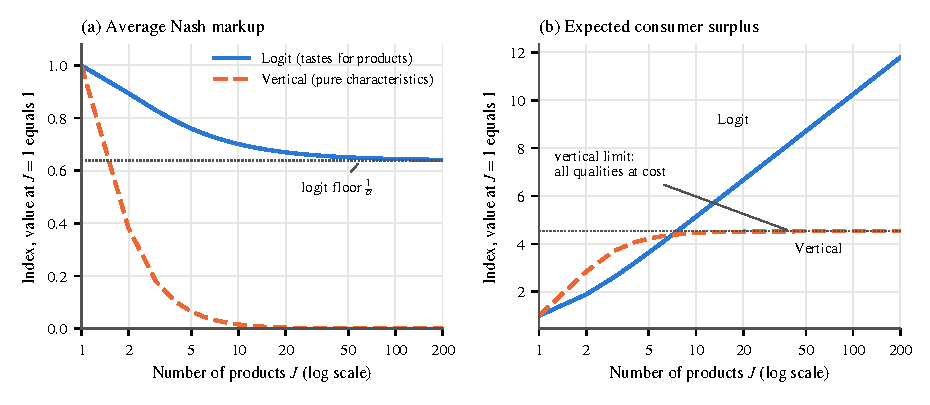
\includegraphics[width=\textwidth]{figures/ch06/clones.pdf}
\caption{Average Nash markup and expected consumer surplus as products are added, in a logit model with identical
products and in a vertical model whose products fill a fixed quality interval. Each product has its own owner. The
logit has $u_{ij} = 2 - p_j + \epsilon_{ij}$, outside good $u_{i0} = \epsilon_{i0}$ and marginal cost $1$. The vertical model
uses Bresnahan's form (\cref{sec:06-bresnahan}), with utility $v\delta_j - p_j$ and $v$ uniform on $[0,1]$. Its
qualities sit at the midpoints of $J$ equal bins of $[1,3]$, marginal cost is $0.05\,e^{\delta}$, and the outside good
has $\delta_0 = p_0 = 0$. Each series is
divided by its value at $J = 1$ because the units of the two models are not comparable. The figure is qualitative.
Computed with \texttt{figures/ch06/src/clones.py}.}
\label{fig:06-clones}
\end{figure}

\Cref{fig:06-clones} computes both models as single-product firms are added. In the logit, the markup falls from
$1.567$ at $J = 1$ to $1.005$ at $J = 200$ and approaches the floor $\frac{1}{\alpha} = 1$. Surplus rises from $0.449$ to
$5.298$ and keeps rising linearly in $\ln J$. In the vertical model, the sales-weighted markup falls from $0.815$ at $J =
1$ to $0.013$ at $J = 10$ and to $0.00003$ at $J = 200$. Surplus converges to $0.752$, the surplus when every quality in
$[1,3]$ is sold at marginal cost.

\subsection{Why the distinction matters}\label{sec:06-eps-matters}

The first implication concerns new goods and price indexes. Retrospective measurement of the gains from new products
goes back to \citet{Trajtenberg1989}, who used a nested logit to value innovations in computed tomography scanners.
Such measurement is also part of constructing ideal price indexes. \citet{BerryPakes2007} note that, according to the Boskin
Commission \citep{BoskinEtAl1996}, failing to measure these gains is the major source of bias in the Consumer Price
Index. A model with tastes for products credits every new variety with a
surplus gain through \eqref{eq:06-logit-gain}, however close it is to existing goods.

\citet[p.~230]{Hausman1997} puts the objection directly. The independence of irrelevant alternatives, he writes,
``typically leads to a vast overestimate of the consumer's surplus from a new good.'' The logit fails to ``incorporate
sufficiently the similarities to existing goods.'' Logit and constant elasticity of substitution demand are positive at every finite price, so the reservation
price at which a new good's demand would vanish is infinite. \citet{Petrin2002} quantifies the role of the shock for
the minivan. His average compensating variation for minivan buyers is \$13,652 with an OLS logit and \$7,414 with an
instrumented logit (1982--84 dollars, his Table~8). It falls to \$3,171 with random coefficients and to \$1,247 when
micro moments are added. The part attributed to the logit error falls from \$95,121 to \$396 across the same columns.
\Cref{ch:newgoods} treats these studies in full.

The second implication concerns market structure. With tastes for products, markups never vanish however many
products crowd the market, so there is always a further incentive to develop products. Market outcomes do not approach
competition as the number of products grows \citep[p.~7]{BerryPakes2007}. A researcher studying a market with hundreds
of products, or the welfare effect of entry, imposes these properties by choosing the model.

\subsection{What the idiosyncratic shock buys}\label{sec:06-eps-advantages}

Models with tastes for products have three practical advantages \citep[pp.~7--8]{BerryPakes2007}. Their choice
probabilities are integrals with simple limits of integration, because conditional on the random coefficients the
logit integral is in closed form \citep{McFadden1981}. Their purchase probabilities are positive at every parameter
value and, under regularity conditions, have smooth derivatives. Their market shares can be inverted to recover the
unobserved characteristics $\xi_j$ as a linear function of parameters and data. Instrumental variables can then handle
the correlation between price and $\xi_j$ \citep{BerryLevinsohnPakes1995}.

Pure characteristics models lose each advantage. The set of tastes for which a product is chosen is a polyhedron whose
shape changes with every parameter value. \citet{FeenstraLevinsohn1995} computed these acceptance regions directly, a
calculation that becomes complicated with several characteristics. Shares are zero whenever a product is dominated,
so the share function has flat regions. The inversion requires new arguments, which \cref{sec:06-purechar} develops.

\subsection{Nesting the two models: the modified BLP model}\label{sec:06-nesting}

A natural idea is to nest the two classes and let the data choose. \citet[eqs.~7--8]{BerryPakes2007} introduce a scale
parameter $\sigma_\epsilon \ge 0$,
\begin{equation}\label{eq:06-nest}
  u_{ij} = f_{ij}(\theta) + \sum_{k=1}^{K} \nu_{ik} X_{jk} + \sigma_\epsilon \epsilon_{ij},
\end{equation}
with $\epsilon_{ij}$ independent standard Gumbel. The model with tastes for products is the case $\sigma_\epsilon = 1$,
and the pure characteristics model is the case $\sigma_\epsilon = 0$. For $\sigma_\epsilon > 0$ define $\mu_\epsilon =
\frac{1}{\sigma_\epsilon}$ and multiply all utilities by $\mu_\epsilon$. This leaves choices unchanged. If $F(\nu)$ is the
distribution of $\nu = (\nu_1, \dots, \nu_K)$, the logit formula gives (their eq.~9)
\begin{equation}\label{eq:06-modblp}
  P_{ij}(\theta, \mu_\epsilon) = \int
  \frac{\exp\bigl(\mu_\epsilon\bigl[f_{ij}(\theta) + \sum_{k} \nu_k X_{jk}\bigr]\bigr)}
       {\sum_{q} \exp\bigl(\mu_\epsilon\bigl[f_{iq}(\theta) + \sum_{k} \nu_k X_{qk}\bigr]\bigr)} \,\dd F(\nu).
\end{equation}
We call \eqref{eq:06-modblp} the \emph{modified BLP model}. Formula \eqref{eq:06-modblp} needs $\mu_\epsilon < \infty$,
so no value of $\mu_\epsilon$ reproduces the pure characteristics model exactly. It is reached only as a limit.

\begin{proposition}[Pure characteristics as a limit]\label{prop:06-limit}
Let $U_{ij}(\nu) = f_{ij}(\theta) + \sum_k \nu_k X_{jk}$ and let
\begin{equation*}
  P^{pc}_{ij}(\theta) = \int \indic\bigl\{U_{ij}(\nu) > U_{iq}(\nu) \text{ for all } q \ne j\bigr\}\,\dd F(\nu)
\end{equation*}
be the pure characteristics choice probability. Suppose ties have probability zero, that is, $F$ assigns probability
zero to the set of $\nu$ with $U_{ij}(\nu) = U_{iq}(\nu)$ for some $q \ne j$. Then $P_{ij}(\theta, \mu_\epsilon) \to
P^{pc}_{ij}(\theta)$ as $\mu_\epsilon \to \infty$.
\end{proposition}

\begin{proof}
Fix $\nu$ outside the tie set and let $m$ be the unique maximizer of $U_{iq}(\nu)$ over $q$. Divide the numerator and
denominator of the integrand by the numerator to obtain
\begin{equation*}
  \frac{1}{1 + \sum_{q \ne j} \exp\bigl(\mu_\epsilon [U_{iq}(\nu) - U_{ij}(\nu)]\bigr)} .
\end{equation*}
If $j = m$, every exponent is negative and each exponential converges to zero, so the integrand converges to one. If
$j \ne m$, the exponent for $q = m$ is positive and that exponential diverges, so the integrand converges to zero. The
integrand therefore converges to $\indic\{j = m\}$ for $F$-almost every $\nu$. It lies in $[0,1]$, and the constant one
is integrable against the probability measure $F$. The dominated convergence theorem gives the result.
\end{proof}

\citet[footnote~9]{BerryPakes2007} add that a covering argument makes the convergence uniform in $\theta$. One might
hope that estimating $\mu_\epsilon$ along with the other parameters would deliver a large estimate whenever the pure
characteristics model generated the data. \citet[p.~9]{BerryPakes2007} give four reasons to doubt it.
\begin{enumerate}
\item Consistency proofs assume that the true parameter lies in a compact set. One would therefore have to prove
consistency for $\sigma_\epsilon = \frac{1}{\mu_\epsilon}$ on an interval that contains zero. The predicted shares are
undefined at $\sigma_\epsilon = 0$. The objective is then not a continuous function on a compact parameter set that
contains the truth, and the uniform convergence that standard proofs require fails at that boundary.
\item A good approximation needs a small $\sigma_\epsilon$, that is, a large $\mu_\epsilon$. For large $\mu_\epsilon$ the
computer cannot evaluate the exponentials in \eqref{eq:06-modblp}.
\item If $\sigma_\epsilon$ is known to be zero, an estimator that imposes it should estimate the other parameters more
precisely. With market-level data this efficiency gain can matter.
\item To learn whether these problems matter in a given application, one needs an estimator that does not rely on the
approximation \eqref{eq:06-modblp}.
\end{enumerate}
A test of $\sigma_\epsilon = 0$ faces a further, standard difficulty. The null hypothesis lies on the boundary of the
parameter space, where likelihood-ratio and Wald statistics have nonstandard limiting distributions.

\begin{remark}[The two models as bounds]\label{rem:06-bounding}
Real products differ in more than one unobserved characteristic. A pure characteristics model with as many unobserved
characteristics as products contains the model with tastes for products as a special case, by
\eqref{eq:06-dummies}. The pure characteristics model with a single unobserved characteristic and the model with
tastes for products are therefore opposite extremes. \citet[p.~12]{BerryPakes2007} suggest that the two might bound the
effects of unobserved product heterogeneity. Models with several unobserved characteristics are hard to estimate
from market data, although panel data on repeated choices of the same consumers can identify them
\citep{GoettlerShachar2001}.
\end{remark}

\section{Case study: estimating the pure characteristics model}\label{sec:06-purechar}

\citet{BerryPakes2007} turn the pure characteristics model, long used in theory, into an estimable model for market
data. Their paper has no field data. It develops the econometric machinery and then uses Monte Carlo experiments to
compare the pure characteristics model with models that have tastes for products. We follow the order of a case study,
with the simulated designs in the place of a data set.

\subsection{The question}\label{sec:06-bp-question}

The paper asks three questions. Can the pure characteristics model be estimated from market-level data on prices,
quantities and characteristics? How much computation does that take? When do models with tastes for products, possibly
with an estimated scale $\mu_\epsilon$, reproduce the implications of the pure characteristics model for elasticities and
for welfare? The questions matter because welfare analysis of new products extrapolates beyond observed prices. As
\cref{sec:06-epsilon} showed, the two classes of models extrapolate very differently.

\subsection{Model and normalizations}\label{sec:06-bp-model}

Utility of consumer $i$ from product $j = 0, 1, \dots, J$ is (their eq.~10)
\begin{equation}\label{eq:06-bp-u10}
  u_{ij} = x_j \beta_i - \alpha_i p_j + \lambda_i \xi_j ,
\end{equation}
with $\beta_{ik} = \beta_k + \nu_{ik}$, $\alpha_i = \alpha + \nu_{ip} > 0$ and $\lambda_i > 0$. Here $\beta_k$ is the mean
marginal utility of characteristic $k$ and $\nu_{ik}$ is consumer $i$'s deviation from it. Two assumptions are built into
\eqref{eq:06-bp-u10}.

\begin{assumption}[Berry and Pakes, A1 and A2]\label{ass:06-bp}
(A1) There is a single unobserved product characteristic, so $X_j = (x_j, \xi_j) \in \R^K \times \R$. (A2) The unobserved
characteristic is vertical: every consumer prefers more of it.
\end{assumption}

Utility is identified only up to a consumer-specific increasing affine transformation (\cref{prop:06-normalization}).
Berry and Pakes use both degrees of freedom. They subtract $u_{i0}$ from every utility, so the outside option has utility
zero and every characteristic is measured relative to the outside option. They then divide by $\lambda_i$, so the
coefficient on $\xi$ equals one for every consumer. After relabeling the rescaled coefficients, the model is (their
eq.~11)
\begin{equation}\label{eq:06-bp-u11}
  u_{ij} = x_j \beta_i - \alpha_i p_j + \xi_j , \qquad u_{i0} = 0 .
\end{equation}
This is the model of \citet{BerryLevinsohnPakes1995} without the shock $\epsilon_{ij}$. Units remain free. Multiplying
every $\xi_j$, $\beta_i$ and $\alpha_i$ by the same positive constant changes no choice (their footnote~12). Berry and
Pakes set the mean of $\alpha_i$ to one, so utility and $\xi$ are measured in units of the mean price coefficient.

Two interpretive points follow from the normalizations. First, $\xi_j$ measures the unobserved quality of product $j$
relative to that of the outside option (their footnote~11). A rise in average $\xi$ over time may therefore reflect
better products or a worse outside option, which matters for price indexes \citep{PakesBerryLevinsohn1993}. Second,
$\xi_j$ often stands for the combined effect of many minor characteristics (their footnote~4). If consumers differ in
their relative tastes for several unobserved characteristics, \eqref{eq:06-bp-u11} is misspecified.

\subsection{Computing market shares}\label{sec:06-bp-shares}

\casehead{The vertical building block}
Start with the vertical model $u_{ij} = \delta_j - \alpha_i p_j$, where $\delta_j = x_j\beta + \xi_j$ is quality (their
eqs.~12--13). It is the model of \cref{sec:06-vertical} with the price coefficient $\alpha_i$ in the role of the price
sensitivity $\nu_i$. Order the goods by increasing price. \Cref{sec:06-vcutoffs} showed that consumer $i$ buys $j$ if and
only if $\underline\nu_j(\delta, p) < \alpha_i < \bar\nu_j(\delta, p)$, with the general cutoffs
\eqref{eq:06-bp-cutoffs} (their eqs.~14--16). If $F$ is the distribution of $\alpha_i$, the share of product $j$ is
\eqref{eq:06-bp-share} (their eq.~17). We write it as $s_j(x, p, \xi; \theta, F)$ to show its dependence on the data and
on the unknown parameters $\theta$. Any parameter vector that puts a product below the quality-price frontier predicts a zero
share for it. A model with tastes for products never predicts a zero share.

\casehead{Extension to $K$ dimensions}
In \eqref{eq:06-bp-u11} the coefficients on $x$ vary across consumers. Conditional on $\beta_i = \beta$, however, the model
is again vertical in $\alpha_i$, with qualities $\delta_j(\beta) = x_j \beta + \xi_j$ that depend on the draw. Compute the
cutoffs $\bar\nu_j(\beta)$ and $\underline\nu_j(\beta)$ from \eqref{eq:06-bp-cutoffs} with $\delta_j(\beta)$ in place of
$\delta_j$, and integrate over $\beta$ (their eq.~18):
\begin{equation}\label{eq:06-bp-share18}
  s_j(x, p, \xi; \theta, F, G) = \int \bigl[F(\bar\nu_j(\beta) \mid \beta) - F(\underline\nu_j(\beta) \mid \beta)\bigr]\,
  \indic\{\bar\nu_j(\beta) > \underline\nu_j(\beta)\}\, \dd G(\beta) .
\end{equation}
Here $F(\cdot \mid \beta)$ is the distribution of $\alpha_i$ given $\beta_i = \beta$ and $G$ is the distribution of
$\beta_i$. The pure characteristics share function is a mixture of vertical-model share functions. The conditioning
argument avoids computing the region of $(\beta, \alpha)$ space in which a consumer chooses $j$, the route taken by
\citet{FeenstraLevinsohn1995}. The integral over $\beta$ has no closed form, so it is simulated \citep{Pakes1986}. With
$ns$ draws $\beta_1, \dots, \beta_{ns}$ from $G$ and their empirical distribution $G_{ns}$ (their eqs.~19--20),
\begin{equation}\label{eq:06-bp-share20}
  s_j(x, p, \xi; \theta, F, G_{ns}) = \frac{1}{ns} \sum_{r=1}^{ns}
  \bigl[F(\bar\nu_j(\beta_r) \mid \beta_r) - F(\underline\nu_j(\beta_r) \mid \beta_r)\bigr]\,
  \indic\{\bar\nu_j(\beta_r) > \underline\nu_j(\beta_r)\} .
\end{equation}
Berry and Pakes note that if $F$ has a density that is differentiable in the parameters, the simulated share function is
continuously differentiable in the parameters. The simulation adds error to the computed shares, as in
\citet{BerryLevinsohnPakes1995}.

The comparison with the random coefficients logit is instructive. There the first step integrates out $\epsilon_{ij}$
analytically conditional on $\beta_i$, which yields the logit formula. Here the first step integrates out $\alpha_i$
analytically conditional on $\beta_i$, which yields the vertical formula. Both models simulate the remaining
integral. A practical version of \eqref{eq:06-bp-share20} proceeds as follows (their footnote~15).
\begin{enumerate}
\item Draw $\beta_1, \dots, \beta_{ns}$ from $G$ once, and keep the draws fixed across parameter values so that the
objective function is smooth in the parameters.
\item For each draw $r$, compute $\delta_j(\beta_r) = x_j \beta_r + \xi_j$ for $j = 1, \dots, J$, with $\delta_0 = p_0 = 0$.
\item Sort the products by price and drop those that are dominated for this draw, using the frontier algorithm that
follows \cref{prop:06-frontier}. The survivors have decreasing adjacent cutoffs.
\item For each survivor compute $F(\bar\nu_j \mid \beta_r) - F(\bar\nu_{j+1} \mid \beta_r)$ with cutoffs between adjacent
survivors. Assign zero to the dropped products.
\item Average the conditional shares over the $ns$ draws.
\end{enumerate}
In the Monte Carlo design of \cref{sec:06-bp-design}, $\ln\alpha_i = \sigma_p \nu_{ip}$ with $\nu_{ip}$ standard normal and
independent of $\beta_i$. Step 4 then uses $F(a \mid \beta) = \Phi\bigl(\frac{\ln a}{\sigma_p}\bigr)$ for $a > 0$, with $\Phi$
the standard normal distribution function.

\subsection{Existence and uniqueness of the inverse}\label{sec:06-bp-inverse}

Estimation follows the three steps of \citet{BerryLevinsohnPakes1995}. For each parameter vector one recovers the
unobserved characteristics from the observed shares, computes them with an algorithm, and then chooses the parameters
that best satisfy moment conditions on $\xi$. The first step requires that the share equations have exactly one
solution.

Fix $(x, p, \theta, F, G)$ and write $\sigma_j(\xi_0, \xi)$, $j = 0, 1, \dots, J$, for the share of good $j$ as a function of
the unobserved characteristics of all goods, the outside good included. Let $s^o$ be the observed share vector, assumed
to lie in the interior of the unit simplex, so that every share is strictly between zero and one. With the normalization
$\xi_0 = 0$, we seek $\xi \in \R^J$ such that (their eq.~21)
\begin{equation}\label{eq:06-bp-system}
  \sigma(0, \xi) = s^o .
\end{equation}
For good $j \ge 1$ define the \emph{element-by-element inverse} $r_j(\xi_{-j})$ as the value of $\xi_j$ that matches good
$j$'s share when the other inside goods are held at $\xi_{-j}$ (their eq.~23):
\begin{equation}\label{eq:06-bp-r}
  \sigma_j\bigl(0, r_j(\xi_{-j}), \xi_{-j}\bigr) = s^o_j .
\end{equation}
Stack the inverses into $r(\xi) = (r_1(\xi_{-1}), \dots, r_J(\xi_{-J}))$, a map from $\R^J$ to $\R^J$. A vector $\xi$ solves
\eqref{eq:06-bp-system} if and only if it is a fixed point (their eq.~24)
\begin{equation}\label{eq:06-bp-fixedpoint}
  \xi = r(\xi) .
\end{equation}
Indeed, a fixed point matches every inside share, and the outside share then matches because shares sum to one.

\begin{theorem}[Berry and Pakes 2007, Theorem~1]\label{thm:06-bp-inverse}
Suppose the share function $\sigma$ has the following properties.\footnote{\citet{BerryPakes2007} state monotonicity in
weak form and the substitutes condition as the pair of inequalities in their eqs.~25--26. We add strict monotonicity in
own $\xi$ on the interior, which makes the element-by-element inverse single valued. We also state the substitutes
condition in the form that the proof uses. \citet{BerryGandhiHaile2013} generalize conditions of this type under the
name ``connected substitutes''.}
\begin{enumerate}[label=(\arabic*)]
\item \emph{Monotonicity.} Each $\sigma_j$, $j = 0, \dots, J$, is continuous, nondecreasing in its own $\xi_j$ and
nonincreasing in every other component. It is strictly increasing in $\xi_j$ at any point where $0 < \sigma_j < 1$. For
fixed values of the other components, $\sigma_j \to 0$ as $\xi_j \to -\infty$ and $\sigma_j \to 1$ as $\xi_j \to \infty$.
\item \emph{Linearity of utility in $\xi$.} Raising $\xi$ for every good, the outside good included, by the same amount
changes no share: $\sigma(\xi_0 + c, \xi + c\mathbf{1}) = \sigma(\xi_0, \xi)$ for every $c \in \R$.
\item \emph{Substitutes with some other good.} Let $(\xi_0, \xi)$ give interior shares. Let $(\tilde\xi_0, \tilde\xi) \ge
(\xi_0, \xi)$ componentwise, with equality exactly on a nonempty proper subset $I$ of $\{0, 1, \dots, J\}$. Then
$\sigma_j(\tilde\xi_0, \tilde\xi) < \sigma_j(\xi_0, \xi)$ for at least one $j \in I$.
\end{enumerate}
Then for every $s^o$ in the interior of the unit simplex, \eqref{eq:06-bp-system} has exactly one solution $\xi \in \R^J$.
Moreover, $r$ is a weak contraction in the sup norm: $\lVert r(\xi') - r(\xi) \rVert_\infty \le \lVert \xi' - \xi
\rVert_\infty$.
\end{theorem}

Condition (3) says that when the unobserved characteristics of some goods rise, at least one good whose characteristic
did not rise loses share strictly. The proof has five steps. Steps 3 and 4 follow \citet[eqs.~27--31]{BerryPakes2007}.
They attribute existence to the argument in \citet{Berry1994}. Step 5 gives a self-contained existence argument.
Throughout we write the arguments of $\sigma_j$ in the order (outside good, own, other inside goods) when it helps.

\begin{proof}
\emph{Step 1: $r$ is well defined and continuous.} Fix $j$ and $\xi_{-j}$, and let $g(a) = \sigma_j(0, a, \xi_{-j})$. By
condition (1), $g$ is continuous with limits $0$ and $1$. Since $0 < s^o_j < 1$, the intermediate value theorem gives a
solution of $g(a) = s^o_j$. Two solutions $a < a'$ would make $g$ constant at the interior value $s^o_j$ on $[a, a']$,
which strict monotonicity rules out. For continuity of $r_j$, take $h > 0$. Strict monotonicity gives $g(r_j + h) > s^o_j > g(r_j - h)$. By
continuity of $\sigma_j$ in $\xi_{-j}$, both strict inequalities survive small changes in $\xi_{-j}$, which keeps the
solution within $h$ of $r_j$.

\emph{Step 2: $r$ is monotone.} Let $\xi \le \xi'$ and suppose $r_j(\xi'_{-j}) < r_j(\xi_{-j})$ for some $j$. Raising the
rivals from $\xi_{-j}$ to $\xi'_{-j}$ weakly lowers $j$'s share, so
\begin{equation*}
  s^o_j = \sigma_j\bigl(0, r_j(\xi'_{-j}), \xi'_{-j}\bigr) \le \sigma_j\bigl(0, r_j(\xi_{-j}), \xi'_{-j}\bigr)
  \le \sigma_j\bigl(0, r_j(\xi_{-j}), \xi_{-j}\bigr) = s^o_j .
\end{equation*}
The first inequality uses own monotonicity. Both inequalities hold with equality, so $\sigma_j(0, \cdot, \xi'_{-j})$ is
constant at $s^o_j$ on an interval, which contradicts strict monotonicity. Hence $r(\xi) \le r(\xi')$.

\emph{Step 3: $r$ is a weak contraction.} Take $\xi, \xi' \in \R^J$ with $d = \lVert \xi - \xi' \rVert_\infty$, and write
$r_j = r_j(\xi_{-j})$ and $r'_j = r_j(\xi'_{-j})$. By the definition of $r_j$ and linearity with $c = d$,
\begin{equation}\label{eq:06-bp-p27}
  \sigma_j\bigl(d, r_j + d, \xi_{-j} + d\bigr) = \sigma_j\bigl(0, r_j, \xi_{-j}\bigr) = s^o_j .
\end{equation}
Now $\xi'_{-j} \le \xi_{-j} + d$ and $0 < d$. Lowering the rivals' characteristics from $(d, \xi_{-j} + d)$ to $(0,
\xi'_{-j})$ weakly raises $j$'s share, so
\begin{equation}\label{eq:06-bp-p28}
  \sigma_j\bigl(0, r_j + d, \xi'_{-j}\bigr) \ge s^o_j .
\end{equation}
Suppose $r'_j > r_j + d$. Then own monotonicity and \eqref{eq:06-bp-p28} give
\begin{equation*}
  s^o_j = \sigma_j\bigl(0, r'_j, \xi'_{-j}\bigr) \ge \sigma_j\bigl(0, r_j + d, \xi'_{-j}\bigr) \ge s^o_j ,
\end{equation*}
so $\sigma_j(0, \cdot, \xi'_{-j})$ would be constant at $s^o_j$ on $[r_j + d, r'_j]$. This contradicts strict
monotonicity, so $r'_j \le r_j + d$. The same argument with $c = -d$ gives $r'_j \ge r_j - d$. Hence $|r'_j - r_j| \le d$
for every $j$, which is the weak contraction property.

\emph{Step 4: uniqueness.} Suppose $\xi \ne \xi'$ both solve \eqref{eq:06-bp-system}. Exchanging their names if
necessary, $\bar c = \max_k (\xi_k - \xi'_k) > 0$. Let $I = \{k : \xi_k - \xi'_k = \bar c\}$, a nonempty set of inside goods.
Define $\tilde\xi = \xi' + \bar c\mathbf{1}$ and $\tilde\xi_0 = \bar c$. By linearity,
\begin{equation*}
  \sigma(\tilde\xi_0, \tilde\xi) = \sigma(0, \xi') = s^o .
\end{equation*}
Compare $(\tilde\xi_0, \tilde\xi)$ with $(0, \xi)$. For each inside good, $\tilde\xi_k - \xi_k = \bar c - (\xi_k - \xi'_k) \ge
0$, with equality exactly for $k \in I$. For the outside good, $\tilde\xi_0 - 0 = \bar c > 0$. So $(\tilde\xi_0, \tilde\xi) \ge
(0, \xi)$ with equality exactly on $I$, a nonempty proper subset of $\{0, \dots, J\}$. Shares at $(0, \xi)$ equal $s^o$ and are
interior. Condition (3) then yields a good $j \in I$ with $\sigma_j(\tilde\xi_0, \tilde\xi) < \sigma_j(0, \xi) = s^o_j$. But
$\sigma_j(\tilde\xi_0, \tilde\xi) = s^o_j$, a contradiction.

\emph{Step 5: existence.} We first find a vector $\xi^{(0)}$ with $r(\xi^{(0)}) \ge \xi^{(0)}$. By linearity,
$\sigma(0, a\mathbf{1}) = \sigma(-a, \mathbf{0})$. As $a \to -\infty$, the outside good's own characteristic $-a$ goes to
infinity, so by condition (1) its share goes to one and every inside share goes to zero. Choose $a$ with $\sigma_j(0,
a\mathbf{1}) < s^o_j$ for all $j \ge 1$. At own value $a$ and rivals at $a$, good $j$ falls short of its target, so own
monotonicity gives $r_j(a\mathbf{1}_{-j}) > a$. Set $\xi^{(0)} = a\mathbf{1}$ and iterate $\xi^{(n+1)} = r(\xi^{(n)})$. By
Step 2 and induction, the sequence is nondecreasing.

Next, the sequence is bounded. Because it is nondecreasing, it can be unbounded only if some component
diverges to infinity. Since $\xi^{(n)}_j \le r_j(\xi^{(n)}_{-j})$ and $\sigma_j$ increases in own $\xi_j$, every
inside share satisfies $\sigma_j(0, \xi^{(n)}) \le s^o_j$. Shares sum to one, so $\sigma_0(0, \xi^{(n)}) \ge s^o_0 > 0$.
Suppose component $\xi^{(n)}_k$ diverged. Because the other components are at least $\xi^{(0)}_{-k}$ and
$\sigma_0$ is nonincreasing in inside characteristics,
\begin{equation*}
  \sigma_0\bigl(0, \xi^{(n)}\bigr) \le \sigma_0\bigl(0, \xi^{(n)}_k, \xi^{(0)}_{-k}\bigr)
  \le 1 - \sigma_k\bigl(0, \xi^{(n)}_k, \xi^{(0)}_{-k}\bigr) \to 0 ,
\end{equation*}
by the limit in condition (1). This contradicts $\sigma_0 \ge s^o_0$. A bounded nondecreasing sequence converges, say to
$\xi^*$. By continuity of $r$, $\xi^* = \lim r(\xi^{(n)}) = r(\xi^*)$, so $\xi^*$ solves \eqref{eq:06-bp-system}.
\end{proof}

\begin{remark}[The conditions in the pure characteristics model]\label{rem:06-bp-conditions}
\citet[Comment~1]{BerryPakes2007} observe that the conditions hold for any finite $\theta$ as long as $F(\cdot \mid \beta)$
has a positive density. The distribution $G$ need not have a density, so the simulated $G_{ns}$ of
\eqref{eq:06-bp-share20} is allowed. Linearity holds by construction in \eqref{eq:06-bp-u11}, and their Comment~2 notes
that any model that is linear in $\xi$ alone would share the result. Condition (3) can be checked draw by draw.
Conditional on $\beta$, the undominated goods form a chain ordered by price, and each good on the chain competes with its
neighbors. The outside good is always on the chain. If the chain contains goods both inside and outside $I$, some
adjacent pair has one member in each. Raising the characteristic of the member outside $I$ strictly lowers the
conditional share of its neighbor in $I$, because $F$ has a positive density. Interior aggregate shares ensure that
such draws have positive probability.
\end{remark}

Steps 3 to 5 are constructive. The iteration in Step 5 is the element-by-element inverse started from a low point. It
converges monotonically, but the argument gives no rate. The weak contraction property gives no rate either, because its
modulus may equal one. \citet{BerryPakes2007} report that they could not prove a modulus below one. This is the main
computational difference from the logit-based contraction of \citet{BerryLevinsohnPakes1995}, which converges at a
geometric rate.

\subsection{Computing the inverse}\label{sec:06-bp-compute}

Berry and Pakes offer three methods, because each fails in some of their experiments.

\casehead{The modified BLP contraction}
Apply the BLP contraction of \cref{ch:blp} to the modified BLP model \eqref{eq:06-modblp} with a large fixed
$\mu_\epsilon$. Since the logit part of \eqref{eq:06-modblp} depends on mean utility only through $\mu_\epsilon\delta$, the
iteration on mean utilities reads
\begin{equation}\label{eq:06-modblp-contraction}
  \delta^{(h+1)} = \delta^{(h)} + \frac{1}{\mu_\epsilon}\bigl[\ln s^o - \ln s(\delta^{(h)}; \mu_\epsilon)\bigr] .
\end{equation}
The method is fast. It is inaccurate when $\mu_\epsilon$ cannot be set high enough, and numerical overflow limits how
high it can go.

\casehead{The element-by-element inverse}
Start from a candidate vector. For each product $j$, hold the other products at their current values and solve the
one-dimensional monotone equation \eqref{eq:06-bp-r} for $\xi_j$. Update all products and repeat until predicted shares
match observed shares. By \cref{thm:06-bp-inverse} each pass is a weak contraction. In practice the method sometimes
makes large gains in the first iterations and then nearly stops. If predicted shares are then positive, Newton steps can
finish the job.

\casehead{The homotopy}
A homotopy deforms a problem with a known solution into the problem of interest. Berry and Pakes use the fixed-point
homotopy (their eq.~32)
\begin{equation}\label{eq:06-homotopy}
  h(\xi, t, \xi_0) = (1 - t)(\xi - \xi_0) + t\bigl(\xi - r(\xi)\bigr), \qquad t \in [0, 1],
\end{equation}
where $\xi_0$ is a starting guess, for example the output of another method. Let $\xi(t)$ solve $h(\xi, t, \xi_0) = 0$.
At $t = 0$ the solution is $\xi_0$, and at $t = 1$ it is the fixed point \eqref{eq:06-bp-fixedpoint}. Rearranging $h = 0$
gives (their eq.~33)
\begin{equation}\label{eq:06-homotopy33}
  \xi(t) = (1 - t)\,\xi_0 + t\, r\bigl(\xi(t)\bigr) .
\end{equation}

\begin{proposition}[Convergence of the homotopy]\label{prop:06-homotopy}
Under the conditions of \cref{thm:06-bp-inverse}, let $\xi^*$ be the unique solution of \eqref{eq:06-bp-system}.
\begin{enumerate}[label=(\roman*)]
\item For each $t \in [0, 1)$, the map $\Phi_t(\xi) = (1 - t)\xi_0 + t\, r(\xi)$ is a contraction with modulus at most $t$.
Hence $\xi(t)$ exists, is unique, and is the limit of the recursion $\xi \mapsto (1-t)\xi_0 + t\,r(\xi)$ (their eq.~34)
from any starting point.
\item $\lVert \xi(t) - \xi^* \rVert_\infty \le \lVert \xi_0 - \xi^* \rVert_\infty$ for every $t \in [0,1)$, and $\xi(t) \to
\xi^*$ as $t \to 1$.
\end{enumerate}
\end{proposition}

\begin{proof}
For (i), $\lVert \Phi_t(\xi) - \Phi_t(\xi') \rVert_\infty = t \lVert r(\xi) - r(\xi') \rVert_\infty \le t \lVert \xi - \xi'
\rVert_\infty$ by the weak contraction property. The contraction mapping theorem (\cref{app:math}) gives the rest.

For (ii), subtract $\xi^* = (1 - t)\xi^* + t\, r(\xi^*)$ from \eqref{eq:06-homotopy33}:
\begin{equation*}
  \xi(t) - \xi^* = (1 - t)(\xi_0 - \xi^*) + t\bigl[r(\xi(t)) - r(\xi^*)\bigr] .
\end{equation*}
Taking norms and using the weak contraction property,
\begin{equation*}
  \lVert \xi(t) - \xi^* \rVert_\infty \le (1 - t)\lVert \xi_0 - \xi^* \rVert_\infty + t \lVert \xi(t) - \xi^* \rVert_\infty .
\end{equation*}
Collecting terms and dividing by $1 - t > 0$ gives the bound. The path is therefore bounded. Take any sequence $t_n \to 1$
along which $\xi(t_n)$ converges, say to $\hat\xi$. Passing to the limit in \eqref{eq:06-homotopy33} and using continuity of
$r$ gives $\hat\xi = r(\hat\xi)$. By uniqueness $\hat\xi = \xi^*$. Every convergent subsequence has the same limit, so
$\xi(t) \to \xi^*$.
\end{proof}

The modulus $t$ explains the practical behavior. Each tenfold reduction in the error of the recursion takes about
$\frac{\ln 10}{-\ln t}$ iterations. That is about 229 iterations at $t = 0.99$, 459 at $t = 0.995$ and 1,150 at
$t = 0.998$. Berry and Pakes start at $t = 0.99$ and move $t$ toward one slowly, solving for each new $\xi(t)$ by Newton's
method when the recursion becomes slow. They find that the homotopy gets much closer to the solution than the
element-by-element inverse before it slows down.

What the paper calls the ``homotopy'' method is an integrated routine that combines the three methods.
\begin{enumerate}
\item Run the modified BLP contraction \eqref{eq:06-modblp-contraction} with a high $\mu_\epsilon$, lowering
$\mu_\epsilon$ if numerical errors arise.
\item If needed, switch to the element-by-element inverse, with periodic Newton steps when possible.
\item If that does not converge quickly, use the homotopy recursion. For small problems, push $t$ to one or very near it.
For large problems, use only a few values such as $t = 0.99$, $0.995$ and $0.998$.
\end{enumerate}

\subsection{Simulation error and limit theory}\label{sec:06-bp-simerror}

\citet{BerryLintonPakes2004} derive limit theorems as the number of products $J$ grows, for models with and without
tastes for products. The two classes behave very differently, and the difference has computational consequences.

In the plain logit no simulation is needed, but observed shares contain sampling error from a finite sample of
consumers. The inversion is analytic (their eqs.~35--36),
\begin{equation}\label{eq:06-logit-inv-sens}
  \xi_j = \ln s_j - \ln s_0 - x_j \beta , \qquad \frac{\partial \xi_j}{\partial s_j} = \frac{1}{s_j} .
\end{equation}
With many products most shares are small, so the recovered $\xi_j$ are very sensitive to any error in $s_j$.
\citet{BerryLintonPakes2004} show that simulation error causes the same problem in the random coefficients logit. A
back-of-the-envelope calculation shows the orders of magnitude. If $s_j$ is estimated from $n$ independent draws, its
variance is about $\frac{s_j(1 - s_j)}{n}$. The delta method then gives
\begin{equation*}
  \Var(\ln \hat s_j) \approx \frac{1}{s_j^2}\cdot\frac{s_j(1 - s_j)}{n} = \frac{1 - s_j}{n s_j} .
\end{equation*}
With $s_j$ of order $\frac{1}{J}$, the standard deviation of the error in $\xi_j$ is of order $\sqrt{\frac{J}{n}}$. It grows
with the number of products unless $n$ grows faster than $J$.

The pure characteristics model behaves in the opposite way. As products crowd the space, competition becomes local and
fierce, so $\frac{\partial s_j}{\partial \xi_j}$ is large and the inverse map is insensitive to share errors. The
vertical model makes this concrete. By \cref{prop:06-vinversion}, $\delta_j = \sum_{m \le j} (p_m - p_{m-1})
F^{-1}(S_m)$, where $S_m = \sum_{k \ge m} s_k$ is a cumulative share. A cumulative share estimated from $n$ draws has
variance at most $\frac{1}{4n}$, whatever $J$. The weights $\frac{p_m - p_{m-1}}{f(F^{-1}(S_m))}$ translate errors
in $S_m$ into errors in $\delta_j$. Their sum is bounded when prices lie in a bounded interval and the density $f$ is
bounded away from zero there. The error in each $\delta_j$ is then of order $\frac{1}{\sqrt n}$, independent of $J$.

The formal results preserve this ranking, with higher required rates than the heuristic suggests.
\citet{BerryLintonPakes2004} derive conditions for asymptotic normality of the parameter estimates. The number of
simulation draws must grow at rate $J$ in the vertical model and at rate $J^2$ in logit-type models.
\citet[p.~23]{BerryPakes2007} report the Monte Carlo results of that paper. About fifty draws suffice for the limit
distribution to describe the vertical model with up to two hundred products. The logit with one
hundred products requires over two thousand draws.

Two forces therefore pull in opposite directions \citep[pp.~23--24]{BerryPakes2007}. The required number of draws grows
like $J^2$ with tastes for products and like $J$ without them, which favors the pure characteristics model. The BLP
contraction converges geometrically, while no rate is known for the pure characteristics inverse, which favors the
model with tastes for products. Which force dominates depends on the number of products and on how often the inverse
must be computed, which grows with the number of parameters.

\subsection{Estimator, instruments and identification}\label{sec:06-bp-estimator}

Write mean quality as $\delta_j = x_j\beta + \xi_j$ and split the parameters into the linear parameters $\theta_1 = \beta$
and the nonlinear parameters $\theta_2$ that govern the distribution of $(\beta_i - \beta, \alpha_i)$. For each $\theta_2$,
\cref{thm:06-bp-inverse} delivers a unique $\delta(\theta_2)$ that matches the observed shares, computed by the methods of
\cref{sec:06-bp-compute}. The structural error is $\xi_j(\theta) = \delta_j(\theta_2) - x_j\beta$. With instruments $z_j$
satisfying $\E[\xi_j z_j] = 0$, the GMM estimator solves
\begin{equation}\label{eq:06-bp-gmm}
  \hat\theta = \argmin_{\theta} \; \xi(\theta)^\top Z\, W\, Z^\top \xi(\theta),
\end{equation}
where $Z$ stacks the instruments and $W$ is a weighting matrix. The linear parameters can be concentrated out by
instrumental variables regression of $\delta(\theta_2)$ on $x$, exactly as in \cref{ch:blp}.

Price is correlated with $\xi$ in any equilibrium model, so the instruments must exclude it. The small Monte Carlo design
uses five instruments. They are a constant, $x$, $x^2$, the market mean of $x$ and the distance from each product to its
nearest neighbor in $x$. These functions of the characteristics of rival products shift each product's competitive
environment, and so its price and share, without entering its own utility. The distance to the nearest neighbor suits
the pure characteristics model, where substitution is local. An approximation to optimal instruments had little effect
(their footnote~17). The large design uses a constant and $x$, each interacted with market dummies. Berry and Pakes
attribute their success to the requirement that one utility model fit three markets whose product sets differ sharply.

\subsection{The Monte Carlo designs}\label{sec:06-bp-design}

Data are drawn from the model (their eqs.~37--39)
\begin{equation}\label{eq:06-bp-mc}
  u_{ij} = \delta_j + \sigma_x \nu_{ix} x_j - \alpha_i p_j , \qquad
  \ln \alpha_i = \sigma_p \nu_{ip} , \qquad
  \delta_j = \beta_0 + \beta_x x_j + \xi_j ,
\end{equation}
with $(\nu_{ix}, \nu_{ip})$ independent standard normal. The true values are $\sigma_x = 1$, $\sigma_p = 1$, $\beta_0 = 2$ and
$\beta_x = 1$. The price coefficient is lognormal with $\E[\ln \alpha_i] = 0$. This fixes the median of $\alpha_i$ at
one. Its mean is $e^{\frac{\sigma_p^2}{2}} \approx 1.65$ at the true $\sigma_p = 1$. The design therefore normalizes the
median of the price coefficient, while their text describes a normalization of the mean
\citep[p.~11]{BerryPakes2007}.

The characteristic $x$ equals twice a firm-specific uniform $(0,1)$ draw plus one half of a uniform $(0,1)$ draw common to
all firms in the market, which correlates characteristics within a market. Its variance is $\frac{4}{12} + \frac{1}{4}
\cdot \frac{1}{12} = \frac{17}{48} \approx 0.354$. In the base design $\xi_j$ is uniform on $(-\frac{1}{2}, \frac{1}{2})$,
with variance $\frac{1}{12} \approx 0.083$. A second design uses $\xi_j$ uniform on $(-1.5, 1.5)$, with variance $0.75$, which
exceeds the variance of $x$. Price is a convex function of quality, $p_j = \frac{e^{\delta_j}}{20}$. Equivalently, $\delta_j
= \ln(20 p_j)$ is strictly concave in price. In the vertical case this makes the cutoffs strictly decreasing, so every
product sells (\cref{prop:06-frontier}). Since price depends on $\delta_j$ and hence on $\xi_j$, price is endogenous by
construction. Observed shares come from the choices of 5,000 simulated consumers at the true parameters. Prices come
from this formula, and no pricing game is solved, so the design does not need a price equilibrium to exist.
Dividing utility by $\alpha_i$ puts it in the linear form of assumption A1 of \citet{CaplinNalebuff1991}, with type
vector $(\frac{1}{\alpha_i}, \frac{\sigma_x \nu_{ix}}{\alpha_i})$. In the vertical case, $\sigma_x = 0$, the type
$\frac{1}{\alpha_i}$ is lognormal with log-variance $\sigma_p^2 = 1$. It therefore satisfies their assumption A2, which for a
one-dimensional lognormal type holds exactly when the log-variance is at most 2 (\cref{sec:06-branches}). For the
two-dimensional design, A2 would have to be checked for the joint density of this type vector.

The paper uses two sample designs. The small design has 20 markets, each with a number of products drawn with equal
probability from $\{2, \dots, 10\}$, and 100 simulated data sets. The large design is patterned on the evolution of processor
speed in personal computers from 1995 to 1997 \citep{Pakes2003}. It has three markets, or years, with 75, 100 and 125
products. The characteristic $x$ is uniform between the year's minimum and maximum megahertz, divided by ten. The ranges
are 25 to 133 in year 1, 25 to 200 in year 2 and 33 to 240 in year 3. The unobserved characteristic equals the year's
megahertz range times $(2u_j - 1)$, with $u_j$ uniform on $[0, 1]$, so that it scales with $x$. Prices fall over time
(their eq.~40),
\begin{equation}\label{eq:06-bp-mc-price}
  \ln p_j = (t - 1)\ln 0.7 + 1.1 \ln \delta_j ,
\end{equation}
so the price of a given bundle falls about 30 percent a year, and price remains convex in quality. Some shares are very
small, smaller than in typical data sets. The large design uses one data set and asymptotic standard errors. Its
homotopy starts from the output of the modified BLP contraction with fixed $\mu_\epsilon$ and iterates 25 times on (their
eq.~41)
\begin{equation}\label{eq:06-bp-41}
  \delta' = 0.05\,\delta + 0.95\, r(\delta) .
\end{equation}
Recursion \eqref{eq:06-bp-41} anchors on the current $\delta$ instead of a fixed starting point, so it is a damped
element-by-element inverse. Its fixed points are those of $r$.

\subsection{Results}\label{sec:06-bp-results}

\casehead{Computing mean utilities}
\Cref{tab:06-bp-delta} reproduces Table~1 of \citet{BerryPakes2007}. It takes one simulated market with five products
and computes $\delta$ by different methods. The homotopy with the same 5,000 draws that generated the data recovers the
true $\delta$ exactly. With 500 draws it still fits the shares to machine precision, but the $\delta$'s differ from the truth
by 0.15 to 0.23. Their order is preserved. The modified BLP contraction with $\mu_\epsilon = 1$, which is the original BLP
contraction in these units, takes one-fiftieth of the homotopy's time but bears little relation to the truth. With
$\mu_\epsilon = 10$ one value is out of order: $\delta_5 = 4.06$ falls below $\delta_4 = 4.10$. With $\mu_\epsilon = 50$ the
order is right and the errors are 1 to 2 percent, but the time rises to 58 percent of the full homotopy's. With 500
draws and $\mu_\epsilon = 50$ the errors grow to between 0.26 and 0.57, larger than the homotopy's errors with the same
draws.

\begin{table}[htbp]
\centering
\caption{Computing $\delta$ by different methods: one market with five products}
\label{tab:06-bp-delta}
\small
\begin{tabular}{@{}lccccccc@{}}
\toprule
 & True & \multicolumn{2}{c}{Homotopy} & \multicolumn{4}{c}{Modified BLP contraction, fixed $\mu_\epsilon$} \\
\cmidrule(lr){3-4} \cmidrule(l){5-8}
Draws ($ns$) & 5,000 & 5,000 & 500 & 5,000 & 5,000 & 5,000 & 500 \\
$\mu_\epsilon$ & & & & 1 & 10 & 50 & 50 \\
\midrule
$\delta_1$ & 2.99 & 2.99 & 3.14 & 3.08 & 3.02 & 3.04 & 3.25 \\
$\delta_2$ & 3.21 & 3.21 & 3.36 & 2.09 & 3.19 & 3.26 & 3.51 \\
$\delta_3$ & 3.56 & 3.56 & 3.71 & 3.13 & 3.60 & 3.62 & 3.94 \\
$\delta_4$ & 4.04 & 4.04 & 4.27 & 4.13 & 4.10 & 4.10 & 4.61 \\
$\delta_5$ & 4.10 & 4.10 & 4.32 & 2.68 & 4.06 & 4.16 & 4.65 \\
\midrule
Relative time & & 1 & 0.15 & 0.02 & 0.12 & 0.58 & 0.03 \\
\bottomrule
\end{tabular}

\smallskip
\begin{minipage}{0.92\textwidth}
\footnotesize Source: \citet{BerryPakes2007}, Table~1. Data come from model \eqref{eq:06-bp-mc}. The ``True'' column
uses the 5,000 consumer draws that generated the shares. Relative time is computing time relative to the homotopy with
5,000 draws.
\end{minipage}
\end{table}

\casehead{Parameter estimates with few products}
\Cref{tab:06-bp-small} combines Tables~2 and~3 of the paper. With a small variance of $\xi$, the modified BLP
contraction with $\mu_\epsilon$ fixed at 30 does about as well as the homotopy. The means of $\sigma_x$ are 1.04 and 1.03
and those of $\beta_0$ are 2.06 and 2.00. With the larger variance of $\xi$, Berry and Pakes needed $\mu_\epsilon = 50$ for
comparable performance, and computational problems prevented pushing $\mu_\epsilon$ much higher. All methods then
overestimate $\sigma_x$ (1.24 and 1.26) and $\beta_0$ (2.34 and 2.33). In the first experiment $\mu_\epsilon = 30$ worked a
little better than $\mu_\epsilon = 50$, perhaps because of approximation errors in computing exponentials of large
numbers (their footnote~18).

\begin{table}[htbp]
\centering
\caption{Monte Carlo estimates with a small number of products per market}
\label{tab:06-bp-small}
\small
\setlength{\tabcolsep}{4.5pt}
\begin{tabular}{@{}lccccccc@{}}
\toprule
 & & \multicolumn{4}{c}{Fixed or no scale (Table 2)} & \multicolumn{2}{c}{Estimated scale (Table 3)} \\
\cmidrule(lr){3-6} \cmidrule(l){7-8}
 & True & (1) & (2) & (3) & (4) & (5) & (6) \\
Method & & Mod.\ BLP & Homotopy & Mod.\ BLP & Homotopy & Mod.\ BLP & Mod.\ BLP \\
Scale $\mu_\epsilon$ & & 30 & none & 50 & none & estimated & estimated \\
$\xi_j$ uniform on & & $(-\frac{1}{2}, \frac{1}{2})$ & $(-\frac{1}{2}, \frac{1}{2})$ & $(-1.5, 1.5)$ & $(-1.5, 1.5)$
  & $(-\frac{1}{2}, \frac{1}{2})$ & $(-1.5, 1.5)$ \\
\midrule
$\sigma_x$ & 1 & 1.04 & 1.03 & 1.24 & 1.26 & 1.14 & 1.64 \\
           &   & (0.04) & (0.03) & (0.06) & (0.06) & (0.04) & (0.08) \\
$\sigma_p$ & 1 & 1.00 & 0.98 & 1.02 & 1.02 & 1.03 & 1.09 \\
           &   & (0.01) & (0.01) & (0.03) & (0.03) & (0.01) & (0.03) \\
$\beta_0$  & 2 & 2.06 & 2.00 & 2.34 & 2.33 & 2.19 & 2.79 \\
           &   & (0.05) & (0.05) & (0.10) & (0.09) & (0.06) & (0.12) \\
$\beta_x$  & 1 & 0.99 & 1.00 & 1.04 & 1.05 & 1.00 & 1.03 \\
           &   & (0.01) & (0.01) & (0.02) & (0.03) & (0.01) & (0.03) \\
$\mu_\epsilon$, mean & $\infty$ & & & & & 34.08 & 15.50 \\
                    &          & & & & & (3.31) & (1.98) \\
$\mu_\epsilon$, median & $\infty$ & & & & & 17.81 & 4.67 \\
\bottomrule
\end{tabular}

\smallskip
\begin{minipage}{0.95\textwidth}
\footnotesize Source: \citet{BerryPakes2007}, Tables~2 and~3. Entries are means across 100 simulated data sets of 20
markets with 2 to 10 products each. The paper's text describes the numbers in parentheses in Table~2 as standard
deviations of the estimates across samples. The standard error of each mean is then about one tenth of the number shown.
The note to Table~3 calls them estimated standard deviations of the mean estimates. Columns (5) and (6) use 500
simulation draws. In some runs of columns (5) and (6), $\mu_\epsilon$ rose until numerical errors occurred and was then
fixed at 50 (once at 25). The homotopy took about ten times as long as the modified BLP estimates.
\end{minipage}
\end{table}

The numbers in parentheses need care. For Table~2, the paper's text describes them as standard deviations of the
estimates across the 100 samples. The precision of each reported mean is then about one tenth of the number shown. On that
reading, the overestimate of $\sigma_x$ in the high-variance design, about 0.25, is many times the standard error of the
mean. It reflects finite-sample bias, which Monte Carlo noise cannot explain. Berry and Pakes conclude that the asymptotic approximation
understates the variance of the estimator at these sample sizes. They also note that every method does worse when the
unobservable has more variance, so more data are needed for a given precision.

Estimating $\mu_\epsilon$ avoids the need to choose it, but at a cost. With the base variance the estimates move away
from the truth ($\sigma_x = 1.14$, $\beta_0 = 2.19$). With the large variance they are poor ($\sigma_x = 1.64$, $\beta_0 =
2.79$). The estimates of $\mu_\epsilon$ have means of 34.08 and 15.50 and much smaller medians of 17.81 and 4.67. Their
distribution is therefore skewed, and in the high-variance design the typical estimate gives the logit error a large role.
Imposing the traditional logit scale normalization, in place of the normalization on the price coefficient, made
convergence without numerical errors much less likely (their footnote~19).

\casehead{Substitution patterns with few products}
Parameter estimates are rarely the object of interest. \Cref{tab:06-bp-subst} reproduces Table~4 of the paper. It reports
derivatives of the share of the cheapest product in one market of the high-variance design with respect to the prices of
products 1 to 5. Each derivative is computed for every Monte Carlo parameter estimate and then averaged, which
approximates averaging over the sampling distribution of the estimator. The last two columns form a \emph{hybrid}. They
use the parameters estimated by the modified BLP model with estimated $\mu_\epsilon$ but compute derivatives from either
the pure characteristics functional form or the modified BLP form with $\mu_\epsilon = 50$.

\begin{table}[htbp]
\centering
\caption{Derivatives of the share of product 1 with respect to the price of each product}
\label{tab:06-bp-subst}
\small
\begin{tabular}{@{}lcccccc@{}}
\toprule
 & & & \multicolumn{2}{c}{Modified BLP} & \multicolumn{2}{c}{BLP parameters, derivatives via} \\
\cmidrule(lr){4-5} \cmidrule(l){6-7}
Product & True & Homotopy & Fix $\mu_\epsilon = 50$ & Estimate $\mu_\epsilon$ & Homotopy & Mod.\ BLP \\
\midrule
1 & $-0.6027$ & $-0.6198$ & $-0.7313$ & $-0.4130$ & $-0.5241$ & $-0.6353$ \\
  &           & (0.0337)  & (0.0220)  & (0.0232)  & (0.0267)  & (0.0226) \\
2 & 0.1981 & 0.2093 & 0.2531 & 0.1656 & 0.1629 & 0.2034 \\
  &        & (0.0233) & (0.0140) & (0.0139) & (0.0133) & (0.0144) \\
3 & 0.1621 & 0.1624 & 0.1183 & 0.0331 & 0.1461 & 0.1096 \\
  &        & (0.0106) & (0.0022) & (0.0059) & (0.0129) & (0.0024) \\
4 & 0.0000 & 0.0002 & 0.0278 & 0.0348 & 0.0001 & 0.0172 \\
  &        & (0.0001) & (0.0038) & (0.0042) & (0.0001) & (0.0031) \\
5 & 0.0204 & 0.0252 & 0.0292 & 0.0235 & 0.0212 & 0.0296 \\
  &        & (0.0026) & (0.0024) & (0.0023) & (0.0023) & (0.0031) \\
\bottomrule
\end{tabular}

\smallskip
\begin{minipage}{0.95\textwidth}
\footnotesize Source: \citet{BerryPakes2007}, Table~4. Row $k$ gives $\frac{\partial s_1}{\partial p_k}$ for one market of the
design with $\xi$ uniform on $(-1.5, 1.5)$. Entries average the derivative over the Monte Carlo parameter estimates of the
corresponding method. Numbers in parentheses are standard deviations of the calculated sample mean.
\end{minipage}
\end{table}

The homotopy with the pure characteristics functional form reproduces the true pattern far better than either modified
BLP estimate with its own functional form. Even with $\mu_\epsilon$ fixed at 50, the modified BLP model misses the fourth
entry badly, predicting 0.0278 where the truth is zero. Product 4 is not a neighbor of product 1, and only a pure
characteristics model can produce an exact zero. The surprise is the hybrid. The parameters from the modified BLP model
with estimated $\mu_\epsilon$, combined with the pure characteristics functional form, give $-0.5241$, 0.1629, 0.1461, 0.0001
and 0.0212. Berry and Pakes draw two lessons (their p.~31). Good parameter estimates need not produce good predictions
when the model's functional form is used to compute them. Even if one estimates with the modified BLP contraction, one may
not want to use \eqref{eq:06-modblp} to compute implications.

\casehead{Parameter estimates and elasticities with many products}
\Cref{tab:06-bp-large} combines Tables~5 and~6 of the paper. The differences across methods are much larger than with few
products. The modified BLP model with estimated scale does worst. Its estimate $\mu_\epsilon = 0.934$ gives the logit error
a large role, and to match the small shares the constant is driven to $\beta_0 = -6.455$, with a standard error of 66.864. With
$\mu_\epsilon$ fixed (at 10, halved where numerical problems arose), $\beta_0 = 1.354$ is still too low. The homotopy is close
to the truth, with $\beta_0 = 1.956$. The reason is the small shares of this design. A pure characteristics model generates
small shares when products have similar characteristics. A model with tastes for products can generate them only through
very low mean utilities. Twenty-five iterations of \eqref{eq:06-bp-41} raise the mean of the computed $\delta$'s
substantially relative to the modified BLP output.

\begin{table}[htbp]
\centering
\caption{The large design: parameter estimates and own-price elasticities}
\label{tab:06-bp-large}
\small
\begin{tabular}{@{}lcccc@{}}
\multicolumn{5}{@{}l}{\emph{Panel A. Parameter estimates (Table 5)}} \\
\toprule
 & & & \multicolumn{2}{c}{Modified BLP} \\
\cmidrule(l){4-5}
Parameter & True & Homotopy & Fix $\mu_\epsilon$ & Estimate $\mu_\epsilon$ \\
\midrule
$\sigma_x$ & 1 & 0.833 & 0.862 & 0.832 \\
           &   & (0.194) & (0.380) & (6.956) \\
$\sigma_p$ & 1 & 1.192 & 1.188 & 1.207 \\
           &   & (0.556) & (0.621) & (1.783) \\
$\beta_0$  & 2 & 1.956 & 1.354 & $-6.455$ \\
           &   & (2.013) & (2.066) & (66.864) \\
$\beta_x$  & 1 & 0.984 & 0.986 & 0.879 \\
           &   & (0.209) & (0.198) & (1.102) \\
Scale $\mu_\epsilon$ & & $\infty$ & 10 & 0.934 \\
                     & & & & (6.680) \\
\bottomrule
\end{tabular}

\bigskip
\begin{tabular}{@{}rrrrrrr@{}}
\multicolumn{7}{@{}l}{\emph{Panel B. Percent change in share from a 1 percent price increase, five cheapest products of year 1 (Table 6)}} \\
\toprule
 & & & & \multicolumn{2}{c}{Modified BLP} & BLP parameters, \\
\cmidrule(lr){5-6}
Share (\%) & Price & True & Homotopy & Fixed $\mu_\epsilon$ & Est.\ $\mu_\epsilon$ & derivatives via homotopy \\
\midrule
5.2109 & 1.26 & $-11.0$  & $-14.6$  & $-6.8$  & $-1.8$ & $-14.6$ \\
4.0180 & 1.58 & $-26.8$  & $-24.5$  & $-9.2$  & $-2.3$ & $-24.7$ \\
0.1078 & 2.93 & $-30.8$  & $-46.3$  & $-11.0$ & $-2.9$ & $-45.3$ \\
0.0038 & 3.85 & $-100.0$ & $-100.0$ & $-14.8$ & $-3.7$ & $-100.0$ \\
0.8855 & 4.01 & $-63.4$  & $-58.5$  & $-19.3$ & $-4.9$ & $-57.9$ \\
\bottomrule
\end{tabular}

\smallskip
\begin{minipage}{0.95\textwidth}
\footnotesize Source: \citet{BerryPakes2007}, Tables~5 and~6. One simulated data set with three markets of 75, 100 and 125
products. Asymptotic standard errors in parentheses. The fixed scale was set to 10 and halved for parameter values and
markets that caused numerical problems, in a few cases down to 2.5. Elasticities in Panel B are computed from a discrete
1 percent price change. The last column of Panel B takes the $\sigma$ estimates of the modified BLP model with estimated
scale. It recomputes $\delta$ with the homotopy contraction and $\beta$ from the new $\delta$, and it uses the pure
characteristics functional form.
\end{minipage}
\end{table}

Panel B shows the implications. All methods capture the general pattern of substitution, although the modified BLP
model is more diffuse. Only the homotopy captures the level of the elasticities. The products with very small shares have
excellent substitutes in the pure characteristics model. For the fourth product, with a share of 0.0038 percent, a 1
percent price increase wipes out all sales, an elasticity of $-100$. The modified BLP model with estimated scale predicts
$-3.7$ for the same product, and the model with fixed scale predicts $-14.8$. Such a product would survive only if a
multi-product firm sold it, so that some markup could be sustained (their footnote~21). The hybrid column again comes
close to the truth. Berry and Pakes read this as evidence that BLP-type estimates can locate the relative importance of
the characteristics even when the data say little about how local substitution is. Holding the $\sigma$'s fixed and taking
$\mu_\epsilon$ to infinity is then a cheap robustness check.

\casehead{Welfare}
\Cref{tab:06-bp-welfare} reports the average gain per person, in dollars, from moving from the year-1 choice set to the
year-3 choice set. Between the two years the number of products rises, quality improves and prices fall, so many consumers
leave the outside good and the true gain is large. All methods do well. The homotopy is within 0.5 percent of the truth
(265.3 against 266.1). The modified BLP model with estimated scale is within 3 percent (259.0). Berry and Pakes explain the
result through share fitting. The contraction fits observed shares exactly, so the extra surplus that the logit errors
would add is offset by lower mean utilities. This roughly cancels the welfare bias of the model with tastes for products.

\begin{table}[htbp]
\centering
\caption{Average welfare gain per person from the year-1 to the year-3 choice set}
\label{tab:06-bp-welfare}
\small
\begin{tabular}{@{}lc@{}}
\toprule
Method & Gain (\$) \\
\midrule
True & 266.1 \\
Homotopy & 265.3 \\
Modified BLP, $\mu_\epsilon = 10$ & 270.0 \\
Modified BLP, $\mu_\epsilon$ estimated & 259.0 \\
Modified BLP, $\mu_\epsilon$ estimated, final homotopy contraction & 272.1 \\
\bottomrule
\end{tabular}

\smallskip
\begin{minipage}{0.75\textwidth}
\footnotesize Source: \citet{BerryPakes2007}, Table~7. Large design. The rows correspond to the methods of Panel B of
\cref{tab:06-bp-large}.
\end{minipage}
\end{table}

\subsection{Robustness and interpretation}\label{sec:06-bp-interpret}

The robustness evidence lies in the comparison of designs. With few products and a small unobservable variance, every
method recovers parameters and elasticities reasonably well. With a larger unobservable variance, all methods lose
precision and the modified BLP model with estimated scale degrades most. With many products and small shares, only the
pure characteristics computation recovers the level of the elasticities. Two results recur. The functional form used to
compute implications matters at least as much as the parameter estimates. Welfare changes between two observed choice
sets are robust in this design because both models fit the observed shares exactly.

We read the welfare result as specific to its setting. Both choice sets are observed and both models are fit to them.
The logit's mechanical credit for variety is then absorbed into lower mean utilities. A counterfactual that adds or
removes products without observed shares to discipline the mean utilities would not have this protection. That is where
\cref{prop:06-logit-exhaust} predicts the largest differences.

\citet[pp.~36--37]{BerryPakes2007} conclude with practical advice. The easiest approach uses the existing BLP method with
their normalization on the price coefficient in place of the usual normalization on the scale of the logit error. It
worked in their experiments when the number of products was not large and the relative variance of $\xi$ was not high.
Fixing $\mu_\epsilon$ at a large value imposes the pure characteristics restriction and gains efficiency by estimating one
parameter fewer. One cannot know in advance how large a value suffices, however, and numerical errors limit how large it
can be. The homotopy is the most accurate method and the slowest. A practical compromise is to estimate by BLP methods and
then compute the implications with the pure characteristics share function. At a minimum this provides a robustness check.

\subsection{Limitations, critiques and contribution}\label{sec:06-bp-critique}

The model allows a single unobserved characteristic, and that characteristic is vertical (\cref{ass:06-bp}). If
consumers differ in their tastes for several unobserved characteristics, the model is misspecified. Market data seem to
offer little scope for estimating richer structures (\cref{rem:06-bounding}). The Monte Carlo evidence is limited: two
designs, one data set in the large design, and prices that are exact functions of mean utility with no cost shocks. The
inverse has no known convergence rate, and the computational burden grows quickly with the number of products. Pure
characteristics models also assume that consumers compare all products. With hundreds of close substitutes this
produces very large elasticities, a point that \citet{BajariBenkard2005} confront directly in \cref{sec:06-bb-pc}.
\citet{Song2007} applies the pure characteristics model to the market for computer processors and compares its welfare
measures with those of a random coefficients logit.

The paper made the theoretical class of pure characteristics models usable with market data. It showed how to compute
shares by conditioning on all but one random coefficient, and it proved that shares can be inverted under weak conditions.
The proof became a template for later invertibility results \citep{BerryGandhiHaile2013}. It provided algorithms with
known properties and documented their trade-offs. It also showed that the choice of functional form for computing
elasticities and welfare can matter more than the estimation method. Above all, it framed the question of what the
idiosyncratic shock assumes about the world and how much the answers to applied questions depend on it.

\section{The hedonic approach}\label{sec:06-hedonic}

The hedonic approach also drops the idiosyncratic shock, but it starts from prices. Each product is a bundle of
characteristics, and the market prices bundles. The relationship between price and characteristics reveals, at each
chosen bundle, the buyer's marginal willingness to pay. We first develop the classical model of \citet{Rosen1974} and the
identification problems raised against it. We then study \citet{BajariBenkard2005}, who adapt the approach to
oligopolistic markets with an unobserved characteristic and a finite number of products.\footnote{Numbers are taken from
the January 2004 working-paper version of \citet{BajariBenkard2005}, NBER Working Paper 10278. All the numbers we cite for
it refer to that version. These are its pages, footnotes, equations (1, 6--18, 21--22 and 29--34), assumptions A1 to A9,
Theorems 1 to 8, Appendices A and B, tables and figures. The article in the \emph{Journal of Political Economy} reports
a revised application based on bounds, with different tables and figures. The Gibbs-sampler estimates of
\cref{sec:06-bb-pc}, including the taste correlations, elasticities and demand curves, appear only in the working paper.
The working paper's title page lists the authors as Benkard and Bajari.}

\subsection{Rosen's hedonic model}\label{sec:06-rosen}

\casehead{Consumers}
Products are described by a vector of characteristics $z = (z_1, \dots, z_K)$, and a continuum of product types is
available. In this subsection we follow Rosen and write characteristics as $z$, not as $x$. The market assigns a price $p(z)$ to each bundle. We call $p(\cdot)$ the \emph{hedonic price function}.
Consumers take it as given. A consumer with income $y$ and taste parameter $a$ buys one unit of one product and spends the
rest on a numeraire $c$:
\begin{equation}\label{eq:06-rosen-consumer}
  \max_{c, z}\; U(c, z; a) \quad\text{subject to}\quad c + p(z) = y .
\end{equation}
Substituting the budget constraint and differentiating with respect to $z_k$ gives the first-order condition
\begin{equation}\label{eq:06-rosen-foc}
  \frac{\partial p(z)}{\partial z_k} = \frac{U_{z_k}(y - p(z), z; a)}{U_c(y - p(z), z; a)}, \qquad k = 1, \dots, K .
\end{equation}
At the chosen bundle, the \emph{implicit price} of each characteristic equals the consumer's marginal rate of substitution
between that characteristic and money.

Rosen describes preferences through the \emph{bid function} $\theta(z; u, y, a)$, the amount the consumer would pay for
bundle $z$ and still reach utility $u$. It is defined by
\begin{equation}\label{eq:06-rosen-bid}
  U\bigl(y - \theta(z; u, y, a), z; a\bigr) = u .
\end{equation}
In this section $\theta$ denotes Rosen's bid function. It is unrelated to the parameter vector $\theta$ of
\cref{sec:06-rum}.
Implicit differentiation gives $\theta_{z_k} = \frac{U_{z_k}}{U_c} > 0$ and $\theta_u = -\frac{1}{U_c} < 0$. A higher bid
curve corresponds to lower utility. The consumer reaches the highest utility $u^*$ whose bid curve still touches the price
function. At the optimum $z^*$,
\begin{equation}\label{eq:06-rosen-tangency}
  \theta(z^*; u^*, y, a) = p(z^*), \qquad \theta_{z_k}(z^*; u^*, y, a) = p_{z_k}(z^*), \qquad \theta(z; u^*, y, a) \le p(z) \text{ for all } z .
\end{equation}
The bid curve is tangent to the price function from below.

\casehead{Producers}
A firm with technology parameter $b$ can produce bundle $z$ at unit cost $C(z; b)$ under constant returns. Its
\emph{offer function} $\phi(z; \pi, b) = C(z; b) + \pi$ is the price at which it would supply $z$ and earn profit $\pi$ per
unit. The firm chooses the bundle that maximizes $p(z) - C(z; b)$. At the optimum, with maximal profit $\pi^*$,
$\phi(z; \pi^*, b) \ge p(z)$ for every $z$, with equality at the chosen bundle. The offer curve is tangent to the price
function from above. With general returns to scale the offer function also embeds the optimal output, but the tangency is
the same \citep{Rosen1974}.

\casehead{Equilibrium}
The price function clears the market for every bundle: the distribution of bundles demanded equals the distribution
supplied. In equilibrium $p(z)$ is an envelope of the bid functions of all consumers, which touch it from below. It is also an
envelope of the offer functions of all firms, which touch it from above. \Cref{fig:06-hedonic} draws the geometry. The gradient of the price
function at a traded bundle equals both the marginal willingness to pay of its buyer and the marginal cost of its seller.
The price function is an equilibrium locus. It is neither a demand curve nor a supply curve.

\begin{figure}[htbp]
\centering
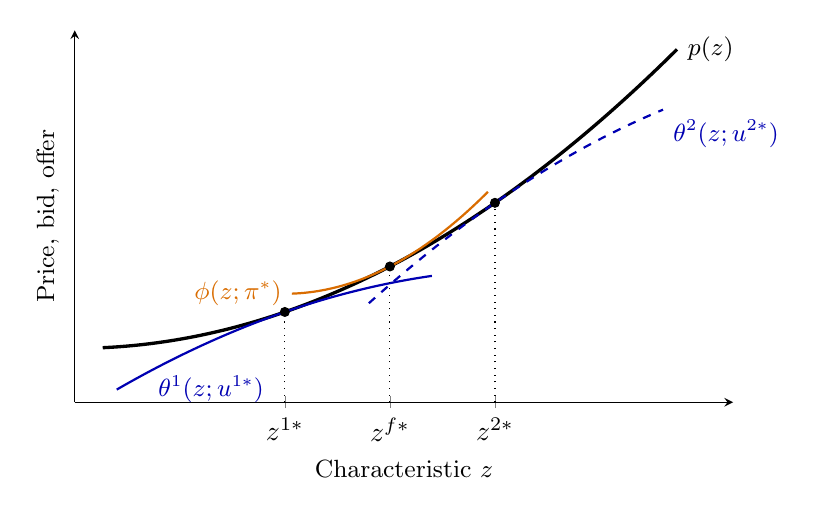
\begin{tikzpicture}
\begin{axis}[
  width=0.82\textwidth, height=0.52\textwidth,
  axis lines=left, xmin=0, xmax=4.7, ymin=0, ymax=6.9,
  xlabel={Characteristic $z$}, ylabel={Price, bid, offer},
  xtick={1.5,2.25,3}, xticklabels={$z^{1*}$, $z^{f*}$, $z^{2*}$},
  ytick=\empty, clip=false, every axis label/.append style={font=\small}]
  \addplot[domain=0.2:4.3, samples=120, very thick, black] {1+0.3*x^2}
    node[pos=1, right, font=\small] {$p(z)$};
  \addplot[domain=0.3:2.55, samples=80, thick, blue!70!black] {1.675+0.9*(x-1.5)-0.25*(x-1.5)^2};
  \node[anchor=east, font=\small, text=blue!70!black] at (axis cs:1.42,0.24) {$\theta^{1}(z; u^{1*})$};
  \addplot[domain=2.1:4.2, samples=80, thick, blue!70!black, dashed] {3.7+1.8*(x-3)-0.3*(x-3)^2}
    node[pos=1, below right, font=\small] {$\theta^{2}(z; u^{2*})$};
  \addplot[domain=1.55:2.95, samples=80, thick, orange!85!black] {2.51875+1.35*(x-2.25)+0.9*(x-2.25)^2}
    node[pos=0, left, font=\small] {$\phi(z; \pi^*)$};
  \addplot[only marks, mark=*, mark size=1.6pt] coordinates {(1.5,1.675) (2.25,2.51875) (3,3.7)};
  \draw[dotted] (axis cs:1.5,0) -- (axis cs:1.5,1.675);
  \draw[dotted] (axis cs:2.25,0) -- (axis cs:2.25,2.51875);
  \draw[dotted] (axis cs:3,0) -- (axis cs:3,3.7);
\end{axis}
\end{tikzpicture}
\caption{The hedonic price function $p(z)$. Consumer 1 and consumer 2 choose $z^{1*}$ and $z^{2*}$, where their bid curves
$\theta^{1}$ and $\theta^{2}$ (concave) touch $p(z)$ from below. A firm chooses $z^{f*}$, where its offer curve $\phi$ touches
$p(z)$ from above. At each traded bundle the slope of $p(z)$ equals the buyer's marginal willingness to pay and the seller's
marginal cost.}
\label{fig:06-hedonic}
\end{figure}

\casehead{Rosen's two-step procedure}
The model suggests two steps. First, regress the prices of products in a market on their characteristics with a flexible
functional form. This yields an estimate $\hat p(z)$ and implicit prices $\hat p_{z_k}(z_j)$ at each traded bundle. Second,
treat the implicit prices as observed marginal prices. Estimate the marginal bid functions $\hat p_{z_k}(z_j) =
F^k(z_j, Y_{1j})$, which depend on characteristics and buyer attributes $Y_{1j}$. Estimate them jointly with the marginal
offer functions $\hat p_{z_k}(z_j) = G^k(z_j, Y_{2j})$, which depend on seller attributes $Y_{2j}$.

\casehead{The identification critique}
The second step runs into two problems, which a one-characteristic example makes transparent. Let the price function be
quadratic,
\begin{equation*}
  p(z) = \pi_0 + \pi_1 z + \tfrac{1}{2}\pi_2 z^2 , \qquad \pi_2 > 0 ,
\end{equation*}
so the implicit price is $p_z(z) = \pi_1 + \pi_2 z$. The coefficients $\pi_0, \pi_1, \pi_2$ are unrelated to the profit $\pi$ of the offer function. Let consumer $i$'s marginal bid be linear,
\begin{equation*}
  \theta_z(z) = b_0 - b_1 z + b_2 Y_i + \eta_i , \qquad b_1 > 0 ,
\end{equation*}
where $Y_i$ is an observed attribute and $\eta_i$ an unobserved taste. The first-order condition $p_z(z_i) = \theta_z(z_i)$
gives
\begin{equation}\label{eq:06-rosen-choice}
  \pi_1 + \pi_2 z_i = b_0 - b_1 z_i + b_2 Y_i + \eta_i
  \quad\Longrightarrow\quad
  z_i = \frac{b_0 - \pi_1 + b_2 Y_i + \eta_i}{\pi_2 + b_1} .
\end{equation}

The first problem was raised by \citet{BrownRosen1982}. In one market the constructed implicit price $\pi_1 + \pi_2 z_i$ is
an exact linear function of $z_i$. Regressing it on $z_i$ and $Y_i$ fits perfectly with coefficients $(\pi_1, \pi_2, 0)$. The
second step merely reproduces the first-step price function and reveals nothing about the slope $-b_1$ of the marginal bid
curve. Identification requires restrictions that the data cannot supply in a single market, such as different functional
forms for the price function and the marginal bid function.

The second problem was stressed by \citet{Epple1987} and \citet{Bartik1987}. By \eqref{eq:06-rosen-choice}, the chosen
quantity $z_i$ rises with the unobserved taste $\eta_i$. Consumers who value the characteristic more buy more of it, and
along a nonlinear price function they also pay a higher implicit price. The regressor $z_i$ is correlated with the error of
the marginal bid equation. The consumer's own attributes are poor instruments, because they enter the bid function or may
correlate with unobserved tastes. A valid instrument must shift the price function that the consumer faces without
shifting tastes. Variation in $(\pi_1, \pi_2)$ across separate markets with the same distribution of tastes does this. In
market $m$ the first-order condition reads $\pi_{1m} + \pi_{2m} z_i = b_0 - b_1 z_i + b_2 Y_i + \eta_i$, and market indicators
identify $b_1$ through their effect on $z_i$.

\citet{EkelandHeckmanNesheim2004} show that the linear-quadratic structure behind the critique is special. Equilibrium
price functions are generically nonlinear, and with additive separability assumptions this nonlinearity can identify
preferences from a single market with one observed characteristic. Rosen's framework also connects to earlier sections.
Bresnahan's quality index $\delta(x) = \sqrt{\beta_0 + \sum_k x_k\beta_k}$ is read as a hedonic expansion path of
cost-minimizing characteristics, and his non-nested tests include a hedonic alternative (\cref{sec:06-bresnahan}).

\subsection{Bajari and Benkard: the model and the price function}\label{sec:06-bb-model}

\casehead{Motivation}
\citet[pp.~1--5]{BajariBenkard2005} give two reasons why hedonic models are rarely used in industrial organization. First,
Rosen assumes perfect competition and a continuum of products. Yet oligopoly is often the object of study, and oligopolistic
markets rarely contain more than a few hundred products. Under imperfect competition a hedonic price function need not
exist, and where it exists it is unlikely to be additively separable. Second, Rosen assumes that every characteristic is observed. In their data on personal computers,
357 of the 695 products are dominated. For each of them, another product is better in every observed characteristic and
cheaper. No hedonic model with full observability can rationalize positive demand for such products. Discrete choice models
avoid the problem through the shock $\epsilon_{ij}$. Bajari and Benkard instead add one characteristic that consumers see and
the econometrician does not.

They contrast their model with BLP-type models along the lines of \cref{sec:06-epsilon}. An i.i.d.\ shock makes the
characteristic space infinite dimensional. Together with the distributional assumptions, it typically produces demand curves
of hyperbolic shape that approach both axes. The hedonic model restricts demand only to slope downward, so the two models can
differ sharply when demand is predicted at prices outside the data.

\casehead{The model}
A product $j$ is a vector $(x_j, \xi_j)$, with $x_j \in \R^K$ observed by consumers and econometrician and a scalar $\xi_j$
observed by consumers only. Markets are indexed by $t \in \mathcal{T}$ and prices by $p_{jt}$. Consumer $i$ has utility
$u_i(x_j, \xi_j, c)$ over the product and a composite good $c \ge 0$ with price one. With income $y_i$, the consumer solves
(their eq.~1)
\begin{equation}\label{eq:06-bb-consumer}
  \max_{(j, c)}\; u_i(x_j, \xi_j, c) \quad\text{subject to}\quad p_{jt} + c \le y_i .
\end{equation}

\begin{assumption}[Bajari and Benkard, A1 to A3]\label{ass:06-bb}
For every consumer and market: (A1) $u_i$ is continuously differentiable and strictly increasing in $c$, with
$\frac{\partial u_i}{\partial c} \ge \underline{m} > 0$ for $c \in (0, y_i]$. (A2) $u_i$ is Lipschitz continuous in $(x_j,
\xi_j)$ with constant $L$. (A3) $u_i$ is strictly increasing in $\xi_j$.
\end{assumption}

We state the bounds $\underline{m}$ and $L$ as common to all consumers, which the Lipschitz property of the price function
requires. Assumption A3 is the strongest. It rules out satiation in the unobserved characteristic.

\begin{theorem}[Bajari and Benkard, Theorem~1]\label{thm:06-bb-pricefn}
Under \cref{ass:06-bb}, for any two products $j$ and $j'$ with positive demand in market $t$:
\begin{enumerate}[label=(\roman*)]
\item If $x_j = x_{j'}$ and $\xi_j = \xi_{j'}$, then $p_{jt} = p_{j't}$.
\item If $x_j = x_{j'}$ and $\xi_j > \xi_{j'}$, then $p_{jt} > p_{j't}$.
\item $|p_{jt} - p_{j't}| \le \bar L\bigl(\lVert x_j - x_{j'} \rVert + |\xi_j - \xi_{j'}|\bigr)$ with $\bar L = \frac{L}{\underline{m}}$.
\end{enumerate}
\end{theorem}

\begin{proof}
Each part shows that a violation would leave one of the two products with no buyers.

(i) Suppose $p_{jt} > p_{j't}$. A consumer who can afford $j$ gets the same product characteristics from $j'$ with more of the
composite good. By A1 she strictly prefers $j'$, so $j$ has no demand.

(ii) Suppose $p_{jt} \le p_{j't}$. For a consumer who can afford $j'$, A1 and then A3 give
\begin{equation*}
  u_i(x_j, \xi_j, y_i - p_{jt}) \ge u_i(x_j, \xi_j, y_i - p_{j't}) > u_i(x_j, \xi_{j'}, y_i - p_{j't}) ,
\end{equation*}
so $j'$ has no demand.

(iii) Let $d = \lVert x_j - x_{j'} \rVert + |\xi_j - \xi_{j'}|$ and suppose $p_{jt} - p_{j't} > \bar L d$. Take a consumer who can
afford $j$, so $y_i \ge p_{jt}$. Split the utility difference into a change in $c$ and a change in characteristics:
\begin{align*}
  u_i(x_{j'}, \xi_{j'}, y_i - p_{j't}) - u_i(x_j, \xi_j, y_i - p_{jt})
  &= \bigl[u_i(x_{j'}, \xi_{j'}, y_i - p_{j't}) - u_i(x_{j'}, \xi_{j'}, y_i - p_{jt})\bigr] \\
  &\quad + \bigl[u_i(x_{j'}, \xi_{j'}, y_i - p_{jt}) - u_i(x_j, \xi_j, y_i - p_{jt})\bigr] \\
  &\ge \underline{m}\,(p_{jt} - p_{j't}) - L d .
\end{align*}
The first bracket uses the mean value theorem and A1, and the second uses A2. The last expression exceeds $\underline{m} \bar L d -
L d = 0$. Every potential buyer of $j$ strictly prefers $j'$, so $j$ has no demand. Exchanging the roles of $j$ and $j'$
covers the other sign.
\end{proof}

The theorem uses only consumer optimization and the fact that consumers take prices as given. It places no restriction on
the supply side, so it holds under oligopoly and in static or dynamic equilibria. Its conclusions justify writing prices in
market $t$ as an equilibrium \emph{price function} $p_t(x, \xi)$ with $p_{jt} = p_t(x_j, \xi_j)$. Bajari and Benkard stress
what the function is not (their pp.~7--8). It is an equilibrium object that changes whenever any primitive changes: a new
product, a cost shock, a change in ownership. It does not predict the price of a product that is not on the market. It is
specific to each market. Even simple oligopoly models imply that it is nonlinear and not additively separable in $\xi$,
because markups depend on all characteristics. They therefore keep the general form.

\subsection{The first stage: the unobserved characteristic as a price quantile}\label{sec:06-bb-firststage}

The first stage recovers $\xi_j$ from prices. The unobserved characteristic has no natural units and is identified only up
to an increasing transformation. Bajari and Benkard normalize it to be uniform on $[0,1]$, which amounts to measuring it by
its own distribution function. Two further assumptions are needed.

\begin{assumption}[Bajari and Benkard, A4 and A5]\label{ass:06-bb-indep}
(A4) $\xi$ is independent of $x$. (A5) For every market $t$ and every $x$, $p_t(x, \cdot)$ is strictly increasing, with
$\frac{\partial p_t(x, \xi)}{\partial \xi} > \underline{\kappa}$ for all $(x, \xi)$ and some $\underline{\kappa} > 0$.
\end{assumption}

A4 strengthens the mean independence common in the literature. Because $\xi$ enters the price function
nonseparably, the model can still generate patterns that look like heteroskedasticity. Bajari and Benkard note that the
monotonicity in A5 follows from consumer preferences through \cref{thm:06-bb-pricefn}(ii). Let $F_{p_t \mid x = x_0}$ denote the distribution of
prices in market $t$ among products with observed characteristics $x_0$.

\begin{theorem}[Bajari and Benkard, Theorem~2]\label{thm:06-bb-xi}
Suppose prices are observed without error and A4 and A5 hold. Then for each market $t$ the price function $p_t$ is
identified within the class of price functions that are strictly increasing in $\xi$. The unobserved characteristics are
also identified:
\begin{equation}\label{eq:06-bb-xi}
  \xi_j = F_{p_t \mid x = x_j}(p_{jt}), \qquad p_t(x_0, e_0) = F^{-1}_{p_t \mid x = x_0}(e_0) .
\end{equation}
\end{theorem}

\begin{proof}
The argument is a chain of equalities.
\begin{align*}
  F_{p_t \mid x = x_j}(p_{jt}) &= \Pr\bigl(p_t(x, \xi) \le p_{jt} \mid x = x_j\bigr) && \text{(definition)} \\
  &= \Pr\bigl(\xi \le p_t^{-1}(x_j, p_{jt}) \mid x = x_j\bigr) && \text{($p_t(x_j, \cdot)$ strictly increasing)} \\
  &= \Pr\bigl(\xi \le p_t^{-1}(x_j, p_{jt})\bigr) && \text{(A4)} \\
  &= p_t^{-1}(x_j, p_{jt}) && \text{($\xi$ uniform on $[0,1]$)} \\
  &= \xi_j && \text{($p_{jt} = p_t(x_j, \xi_j)$).}
\end{align*}
Here $p_t^{-1}(x, \cdot)$ is the inverse of $p_t(x, \cdot)$. The same chain with $(x_0, p_t(x_0, e_0))$ in place of $(x_j,
p_{jt})$ gives $F_{p_t \mid x = x_0}(p_t(x_0, e_0)) = e_0$. Inverting this identity gives the second equation in
\eqref{eq:06-bb-xi}. Both objects are functions of the observable distribution of prices given characteristics, which
proves identification.
\end{proof}

The unobserved characteristic is the rank of a product's price among products with the same observed characteristics. A
computer priced at the 90th percentile among computers with identical observed specifications has $\xi = 0.9$. Identification
uses a single cross-section, so $\xi_j$ and its distribution may change over time. The first part of the argument follows
\citet{Matzkin2003}. If prices are measured with error, identification requires each product to be observed in many markets,
so that averaging removes the error (their Appendix~A, Theorem~6). The estimator replaces the conditional distribution with
a nonparametric estimate (their eq.~18):
\begin{equation}\label{eq:06-bb-xihat}
  \hat\xi_{jt} = \hat F_{p_t \mid x = x_j}(p_{jt}) .
\end{equation}
Kernel or series estimators can be used. In the application a local linear kernel estimator \citep{FanGijbels1996}
worked best.

Bajari and Benkard offer three alternatives to independence. Under \emph{options packages} (their Theorem~3), products are
grouped into models, such as a particular line of desktop computers, and an options package $x$ is chosen within a model.
All products of a model share the same $\xi$ (their A6), and a baseline package $\bar x$ is available for every model (their
A7). Normalizing $\xi$ given $x = \bar x$ to be uniform, $\xi_j$ is the price quantile of the baseline version of $j$'s model.
The approach is a nonparametric analog of fixed effects. It works in one cross-section even with measurement error, and it
is testable because many products share the same $\xi$.

Under a \emph{rich set of price functions} (their Theorem~4), some market has prices that depend on $\xi$ alone (their A8).
Packaged goods whose flavors all sell at the same price are an example. Prices weakly increase in $x$ and strictly increase
in $\xi$ in every market (their A9). With full support and products observed in many markets, these conditions identify the
ranking of the $\xi_j$. Finally, nonseparable nonparametric instrumental variables methods for triangular systems
\citep{ImbensNewey2009} could replace independence. They require instruments that determine the endogenous observed
characteristics yet are independent of $\xi$, and such instruments are hard to find in product markets.

\subsection{The second stage: preferences}\label{sec:06-bb-secondstage}

With $\xi$ recovered, Bajari and Benkard treat it as an observed characteristic. If demand were observed for every price
function, the results of \citet{MasColell1977} would recover preferences. Data are rarely that rich, and often each consumer
is observed once. Two cases arise.

\casehead{Continuous choice set}
Suppose utility is linear in the logarithms of the characteristics and in the composite good (their eq.~6):
\begin{equation}\label{eq:06-bb-u6}
  u_{ij} = \beta_{i1}\ln x_{1j} + \dots + \beta_{iK}\ln x_{Kj} + \beta_{i\xi}\ln \xi_j + c , \qquad c = y_i - p_t(x_j, \xi_j) .
\end{equation}
If the choice set is a continuum and the choice is interior, the consumer chooses $(x, \xi)$ on the price surface to maximize
\eqref{eq:06-bb-u6}. Differentiating with respect to $x_k$ and $\xi$ gives (their eqs.~7--8)
\begin{equation*}
  \frac{\beta_{ik}}{x_{kj}} = \frac{\partial p_t(x_j, \xi_j)}{\partial x_k}, \quad k = 1, \dots, K, \qquad
  \frac{\beta_{i\xi}}{\xi_j} = \frac{\partial p_t(x_j, \xi_j)}{\partial \xi} .
\end{equation*}
Solving for the tastes gives (their eqs.~9--10)
\begin{equation}\label{eq:06-bb-tastes}
  \beta_{ik} = x_{kj}\,\frac{\partial p_t(x_j, \xi_j)}{\partial x_k}, \qquad
  \beta_{i\xi} = \xi_j\,\frac{\partial p_t(x_j, \xi_j)}{\partial \xi} .
\end{equation}
A single observed choice therefore identifies a consumer's entire taste vector, given the price function and $\xi_j$. Each
taste is the implicit price of the characteristic times the chosen quantity, which is the consumer's willingness to pay, in
dollars, for a unit increase in the logarithm of the characteristic. Pooling consumers' choices traces out the population
distribution of tastes nonparametrically. The precision of these estimates depends only on the first-stage sample.

More generally, write $u_i(x, c) = u(x, y_i - p(x); \beta_i)$ with $\beta_i \in \R^B$ (their eq.~11). The first-order
conditions $\frac{\partial}{\partial x_k} u(x, y_i - p(x); \beta_i) = 0$ define the optimal choice $x(\beta)$. Implicit
differentiation gives $x'(\beta) = -[D_{xx}\bar u]^{-1} D_{x\beta}\bar u$, where $\bar u(x; \beta) = u(x, y_i - p(x); \beta)$
(their eqs.~12--14). Their Theorem~5 states that $\beta_i$ is locally identified when $x'(\beta)$ is locally positive or
negative definite, by the inverse function theorem. With as many taste parameters as characteristics ($B = K$) and $x'(\beta)$
definite everywhere on an open convex set, the map $x(\cdot)$ is one-to-one and tastes are globally identified
\citep{GaleNikaido1965}. One choice identifies at most $K$ random coefficients.

\casehead{Discrete choice set}
With finitely many products, utility maximization yields inequalities. If consumer $i$ chooses product $j$, then (their
eq.~15)
\begin{equation}\label{eq:06-bb-ineq}
  u(x_j, \xi_j, y_i - p_{jt}; \beta_i) \ge u(x_k, \xi_k, y_i - p_{kt}; \beta_i) \quad\text{for all } k \ne j ,
\end{equation}
so $\beta_i$ lies in the \emph{revealed preference set} $A_{ij} = \{\beta : \text{\eqref{eq:06-bb-ineq} holds}\}$ (their
eq.~16). The set typically contains more than one point, so individual tastes are not identified. It can still be small when
the choice set is rich. If every characteristic is continuous and the products fill a compact set, the sets shrink to points as the number
of products grows (their Appendix~B, Theorem~8). Their rate argument is simple. In their Appendix~B, utility
$u(x_j, p_j; \beta_i)$ does not depend on income, and there is no outside option. Each set then depends only on the
product chosen, and the sets for the $J$ products partition the bounded parameter space $\mathcal{B}$. Their average
Lebesgue measure is therefore $\frac{m(\mathcal{B})}{J}$. An outside option would add one more set and leave the rate
unchanged. Consumers who buy
nothing are treated as buying a bundle with zero characteristics at zero price (their eq.~17):
\begin{equation*}
  u(0, 0, y_i; \beta_i) \ge u(x_k, \xi_k, y_i - p_{kt}; \beta_i) \quad\text{for all } k .
\end{equation*}
These conditions are only inequalities, so the tastes of non-purchasers are not point identified even with a continuous
product space.

The sets $A_{ij}$ deliver bounds on the population distribution of tastes. Let $\mathcal{B}(\bar\beta) = \{\beta : \beta \le
\bar\beta\}$. The share of consumers whose whole set $A_{ij}$ lies in $\mathcal{B}(\bar\beta)$ is a lower bound for the taste
distribution function at $\bar\beta$. The share whose set meets $\mathcal{B}(\bar\beta)$ is an upper bound. When utility is
quasi-linear, as in \eqref{eq:06-bb-u6}, income cancels from \eqref{eq:06-bb-ineq}. All buyers of product $j$ then share one
set $A_j$, and product-level quantities suffice for estimation.

\casehead{A Bayesian point estimate and the Gibbs sampler}
For a point estimate, Bajari and Benkard turn the inequalities into a likelihood. Consumer $i$ with tastes $\beta_i$ chooses
$j$ with likelihood (their eq.~21)
\begin{equation}\label{eq:06-bb-lik}
  L(j \mid x, y_i, \beta_i) = \indic\bigl\{u(x_j, y_i - p_j; \beta_i) \ge u(x_k, y_i - p_k; \beta_i) \text{ for all } k \ne j\bigr\} ,
\end{equation}
where $x_j$ now includes $\xi_j$. With a uniform prior on a box $\mathcal{B}$ that contains every $A_{ij}$, the posterior
$\pi(\beta_i \mid j) \propto \indic\{\beta_i \in \mathcal{B}\}\, L(j \mid x, y_i, \beta_i)$ is uniform on $A_{ij}$ (their
eq.~22).

Sampling from a uniform distribution on a set defined by many inequalities is easy coordinate by coordinate. In model
\eqref{eq:06-bb-u6}, choice of $j$ requires, for every $k \ne j$ (their eq.~29),
\begin{equation*}
  \sum_{l} \beta_{il}\ln x_{lj} + y_i - p_j \ge \sum_{l} \beta_{il}\ln x_{lk} + y_i - p_k .
\end{equation*}
Collecting the terms in $\beta_{i1}$ gives
\begin{equation*}
  \beta_{i1}\,(\ln x_{1j} - \ln x_{1k}) \ge \sum_{l \ne 1} \beta_{il}(\ln x_{lk} - \ln x_{lj}) + (p_j - p_k) .
\end{equation*}
Define the ratio
\begin{equation}\label{eq:06-bb-ratio}
  R_k(\beta_{i,-1}) = \frac{\sum_{l \ne 1} \beta_{il}(\ln x_{lk} - \ln x_{lj}) + (p_j - p_k)}{\ln x_{1j} - \ln x_{1k}} .
\end{equation}
If $x_{1j} > x_{1k}$, the denominator is positive and the inequality reads $\beta_{i1} \ge R_k$. If $x_{1j} < x_{1k}$,
dividing by a negative number flips it to $\beta_{i1} \le R_k$. If $x_{1j} = x_{1k}$, the inequality does not involve
$\beta_{i1}$. Given the other coordinates, $\beta_{i1}$ is therefore uniform on $[\beta_{1,\min}, \beta_{1,\max}]$ with
(their eqs.~32--33)\footnote{The working paper prints the price term in eqs.~30--33 as $(y_i - p_j) - (y_i - p_k)$, which
has the opposite sign. The expression here follows from their eq.~29.}
\begin{equation}\label{eq:06-bb-bounds}
  \beta_{1,\min} = \max\Bigl\{\underline b_1,\ \max_{k : x_{1j} > x_{1k}} R_k(\beta_{i,-1})\Bigr\}, \qquad
  \beta_{1,\max} = \min\Bigl\{\bar b_1,\ \min_{k : x_{1j} < x_{1k}} R_k(\beta_{i,-1})\Bigr\},
\end{equation}
where $[\underline b_1, \bar b_1]$ is the range of the first coordinate in the prior box. The other coordinates are
handled in the same way. The sampler proceeds as follows.
\begin{enumerate}
\item Start from a point $\beta_i^{(0)}$ in $A_{ij}$. Bajari and Benkard use the tastes implied by the continuous-case
formulas \eqref{eq:06-bb-tastes} and search nearby when that point violates an inequality.
\item Given $\beta_i^{(s)}$, draw $\beta_{i1}^{(s+1)}$ from the uniform distribution on $[\beta_{1,\min}, \beta_{1,\max}]$
computed at the current values of the other coordinates.
\item Draw each remaining coordinate $l = 2, \dots, K$ in the same way, conditioning on the most recent values of the others.
\item Repeat, discarding an initial set of draws.
\end{enumerate}
Each inequality is linear in $\beta_i$, so $A_{ij}$ is an intersection of half-spaces. It is therefore convex, hence
connected, and standard sufficient conditions for convergence of the sampler hold (their footnote~8). The distribution
function of tastes is estimated by the frequency of draws below each point (their eq.~34),
\begin{equation}\label{eq:06-bb-cdf}
  \hat F(\bar\beta_1, \dots, \bar\beta_K) = \frac{1}{S}\sum_{s=1}^{S} \indic\bigl\{\beta^{(s)}_1 \le \bar\beta_1, \dots, \beta^{(s)}_K \le \bar\beta_K\bigr\} ,
\end{equation}
with draws pooled across consumers. The uniform prior selects one distribution among the many consistent with the data. The
sampler extends to repeated choices, which add inequalities, and to estimation error in $\xi$, by drawing $\xi$ from its
sampling distribution before each run.

\casehead{When independence fails}
If $\xi$ is locally positively correlated with some observed characteristic, the first stage attributes part of the price
effect of $\xi$ to that characteristic. Its implicit price is biased upward and the implicit price of $\xi$ downward. Through
\eqref{eq:06-bb-tastes} the estimated tastes inherit the same biases. Because a product is a bundle of both characteristics,
the biases partly offset in the demand for products. Bajari and Benkard report that they cancel exactly with linear utility
and a linear price function.

\subsection{Application: personal computers, December 1999}\label{sec:06-bb-pc}

\casehead{Data}
The data come from the PC Data Retail Hardware Monthly Report. They contain quantities, average prices and characteristics of
desktop computers for 29 months. The analysis concentrates on December 1999, with 695 models, a cross-section in which
traditional demand methods typically struggle. The data reportedly cover about 75 percent of U.S.\ retail computer sales.
Processor dummies are replaced by a CPU benchmark score, which a regression on chip speed interacted with chip dummies explains
with an $R^2$ of 0.999. The final data contain 19 characteristics. The three main continuous characteristics are the benchmark, RAM
and hard drive capacity. Following their Table~1, the others are MMX, SCSI, CD-ROM, DVD, a network card, a monitor dummy, monitor size, a zip
drive, desktop versus tower, refurbished and no modem. Five operating-system dummies complete the list, one of which is
omitted in the regression. With all characteristics treated as observed, 357 of the 695 products are dominated.
\Cref{tab:06-bb-data} reproduces selected rows of their Table~1, including an OLS hedonic regression.

\begin{table}[htbp]
\centering
\caption{Personal computers, December 1999: summary statistics and a linear hedonic regression}
\label{tab:06-bb-data}
\small
\begin{tabular}{@{}lrrrrr@{}}
\toprule
Variable & Mean & S.D. & Min & Max & OLS coefficient \\
\midrule
CPU benchmark          & 1354.5 & 362.3 & 516 & 2544 & 0.836 \\
RAM (MB)               & 74.0 & 35.1 & 16 & 256 & 3.010 \\
Hard drive (MB)        & 9276.8 & 4850.3 & 2100 & 40000 & 0.008 \\
MMX                    & 0.64 & 0.48 & 0 & 1 & $-56.971$ \\
SCSI                   & 0.01 & 0.08 & 0 & 1 & 310.747 \\
CD-ROM                 & 0.67 & 0.47 & 0 & 1 & 26.478 \\
DVD                    & 0.14 & 0.35 & 0 & 1 & 32.213 \\
Monitor included       & 0.31 & 0.46 & 0 & 1 & 29.625 \\
Monitor size           & 0.75 & 3.27 & 0 & 15 & 22.822 \\
Desktop (not tower)    & 0.17 & 0.37 & 0 & 1 & 25.611 \\
Refurbished            & 0.09 & 0.28 & 0 & 1 & $-144.314$ \\
No modem               & 0.55 & 0.50 & 0 & 1 & 145.169 \\
\midrule
Constant               & & & & & $-590.2$ \\
$R^2$                  & & & & & 0.79 \\
$N$                    & & & & & 695 \\
\bottomrule
\end{tabular}

\smallskip
\begin{minipage}{0.85\textwidth}
\footnotesize Source: \citet{BajariBenkard2005}, Table~1 (working-paper version). The dependent variable of the OLS
regression is price in dollars. Rows not shown are the network card, zip drive and four operating-system dummies (Windows NT
4.0, Windows NT, Windows 98, Windows 95, with Windows 3.1 omitted). The paper reports no standard errors for this regression.
\end{minipage}
\end{table}

\casehead{First stage}
A nonparametric estimator in 19 dimensions is impractical, so the first stage treats three continuous characteristics
nonparametrically: CPU benchmark, RAM and hard drive. The price function is assumed additively separable in the other 16, with
coefficients fixed at the OLS values of \cref{tab:06-bb-data}. Bajari and Benkard argue that many of these are peripherals that
can be bought and sold separately, so arbitrage limits nonseparability. The estimator is \eqref{eq:06-bb-xihat} with a local
linear kernel and a normal kernel. Bandwidths were chosen by eye, which oversmooths relative to the mean-squared-error optimum.
Smooth estimates help because derivatives of the price function supply starting values for the sampler. With a finite product
space, only the $\hat\xi_j$ are needed for the demand system itself.

The unobserved characteristics are precisely estimated (their Table~2). Asymptotic standard errors average 0.010, have median
0.009, and are below 0.018 for 95 percent of products, with a maximum of 0.104. Bootstrap standard errors, from 1,000 samples
drawn with i.i.d.\ sampling of products, average 0.012, have 95th percentile 0.022 and maximum 0.121. For 508 of the 695
products the bootstrap standard error exceeds the asymptotic one. Two features explain the precision. A quantile is easier to
estimate than a density, and the characteristic space is densely filled, so almost every product has close neighbors. The
estimated bias was small and barely changed the ranking of the $\hat\xi_j$, so it was left out.

\casehead{Second stage}
The demand system uses all 19 observed characteristics and $\xi$. Utility is quasi-linear, linear in the logarithms of CPU
benchmark, hard drive, RAM and $\xi$, and linear in the other characteristics and in price. The $\hat\xi_j$ were rescaled so
that budget sets are convex, and other normalizations changed the results little. After discarding initial draws, the sampler
produced 1,000 taste draws per product, a total of 695,000 twenty-dimensional draws. These were reweighted by each product's
sales. Including the initial draws, the computation took about an hour on their Sun Ultra 60 workstation.

The estimated willingness-to-pay distributions (their Figures~1--5) look roughly lognormal except for the CPU benchmark. The
modal marginal willingness to pay is between \$1 and \$2 per megabyte of RAM and about 1.25 cents per megabyte of hard drive.
The data are informative even about the taste for SCSI, a dummy characteristic, because extreme values of one coefficient
require extreme values of others to rationalize a choice. Tastes are strongly positively correlated (their Table~3). The
correlation between the CPU and SCSI coefficients is 0.694, between RAM and hard drive 0.533, and between CPU and RAM 0.510. The
taste for $\xi$ correlates positively with every other taste, from 0.351 with hard drive to 0.477 with RAM. This arises even
though $\xi$ was assumed independent of $x$ in the first stage.

\casehead{Elasticities}
Aggregating the taste draws gives demand curves and elasticities for every product. With all 695 products the median
own-price elasticity $\varepsilon_{jj}$ was about $-100$. Bajari and Benkard read this as a rejection of perfect information. With 695 products,
neighbors are close in price and characteristics, so a fully informed consumer would switch at a tiny price change. Real
consumers search and consider only a handful of products. They therefore re-estimated the model with only the 24 products that
sold at least 5,000 units, a minimum share of 0.75 percent. These products account for 72 percent of sales. Own-price
elasticities then range from $-4$ to $-72$, with a median of $-11$. They caution that the selection retained similar
best-selling products, so these elasticities may still be too large in magnitude.

\begin{table}[htbp]
\centering
\caption{The five best-selling computers in December 1999 and their estimated price elasticities}
\label{tab:06-bb-elast}
\small
\begin{tabular}{@{}llrrrr@{}}
\multicolumn{6}{@{}l}{\emph{Panel A. Characteristics (Table 4)}} \\
\toprule
Model & CPU (benchmark) & RAM & Hard drive & Price (\$) & Sales \\
\midrule
HP Pavilion 6535      & Intel Celeron 466 MHz (1281) & 64 MB & 8.4 GB  & 590 & 71,199 \\
Compaq Presario 5441  & AMD K6-2 475 MHz (1076)      & 64 MB & 8.0 GB  & 540 & 54,449 \\
Compaq Presario 5461  & AMD K6-2 500 MHz (1115)      & 64 MB & 10.0 GB & 727 & 43,029 \\
E-Machines eTower 433 & Celeron 433 MHz (1167)       & 32 MB & 4.3 GB  & 471 & 40,399 \\
HP Pavilion 6545C     & Celeron 500 MHz (1398)       & 64 MB & 13.0 GB & 858 & 34,198 \\
\bottomrule
\end{tabular}

\bigskip
\begin{tabular}{@{}lrrrrr@{}}
\multicolumn{6}{@{}l}{\emph{Panel B. Matrix of price elasticities (Table 5)}} \\
\toprule
 & HP6535 & Compaq5441 & Compaq5461 & E-Machines & HP6545C \\
\midrule
HP6535      & $-4.14$ & 0.12    & 0.00    & 0.43     & 0.28 \\
Compaq5441  & 0.17    & $-5.95$ & 2.98    & 0.73     & 0.55 \\
Compaq5461  & 0.00    & 2.80    & $-8.00$ & 0.85     & 0.11 \\
E-Machines  & 0.61    & 0.69    & 0.91    & $-10.65$ & 0.66 \\
HP6545C     & 0.70    & 0.86    & 0.18    & 1.02     & $-4.46$ \\
\bottomrule
\end{tabular}

\smallskip
\begin{minipage}{0.92\textwidth}
\footnotesize Source: \citet{BajariBenkard2005}, Tables~4 and~5 (working-paper version). Table~4 of the paper prints the
processor as ``AMD A6-2''. Panel A corrects it to the AMD K6-2 chip. Elasticities come from the model estimated on the 24 products
selling at least 5,000 units. The paper does not state whether rows or columns index the product whose price changes.
\end{minipage}
\end{table}

\Cref{tab:06-bb-elast} shows the five best sellers and their elasticity matrix. Two features stand out. The most similar
products substitute most, as the two Compaq models do (2.98 and 2.80). Some cross elasticities are exactly zero: the HP6535 and
the Compaq5461 do not substitute at all, presumably because other products lie between them in characteristic space. A model with
an i.i.d.\ shock cannot produce a zero cross elasticity, since every product keeps some buyers who rank it second.

\begin{figure}[htbp]
\centering
\begin{subfigure}[t]{0.8\textwidth}
\centering
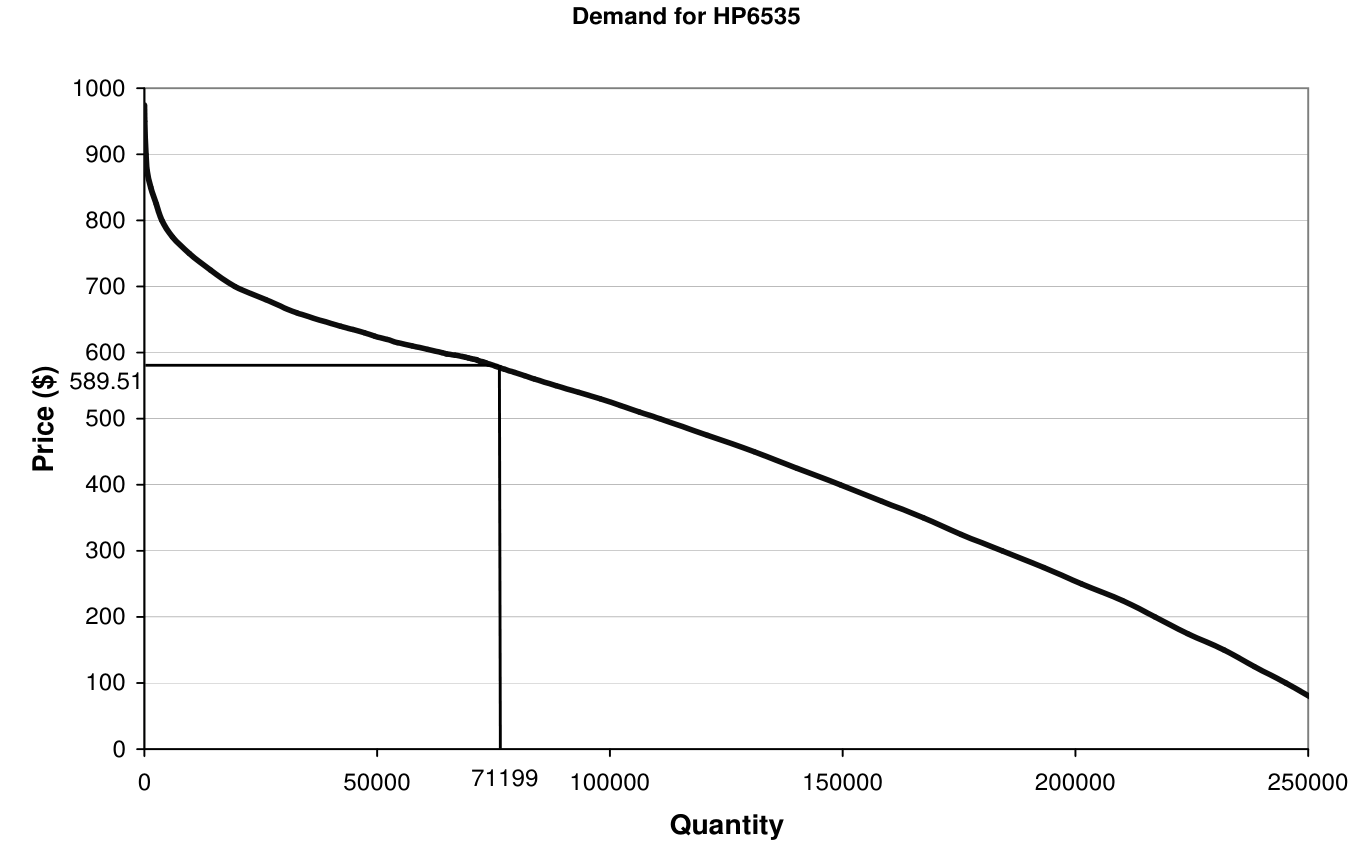
\includegraphics[width=\textwidth]{figures/ch06/bb_fig6_demand.png}
\caption{Estimated demand for the HP Pavilion 6535}
\end{subfigure}\par\medskip
\begin{subfigure}[t]{0.8\textwidth}
\centering
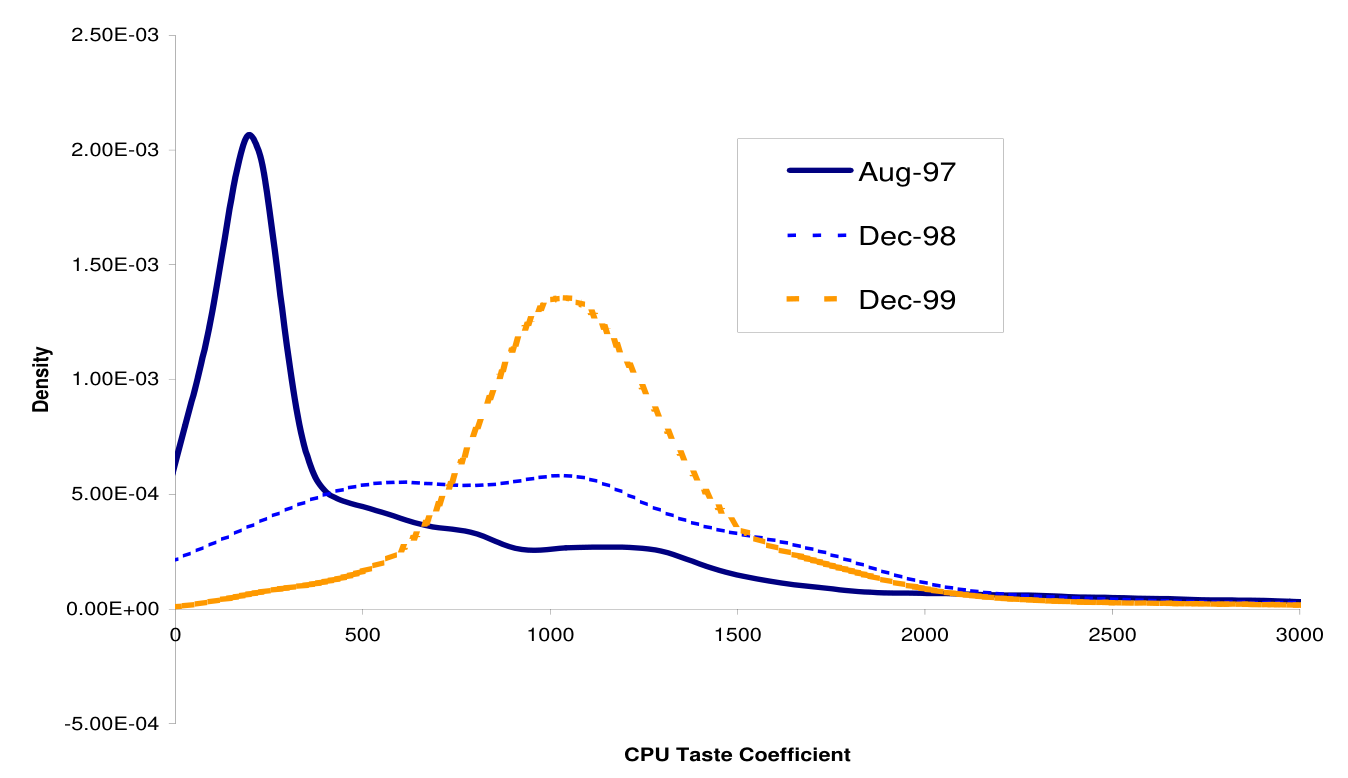
\includegraphics[width=\textwidth]{figures/ch06/bb_fig7_cputaste.png}
\caption{Estimated density of the taste for CPU}
\end{subfigure}
\caption{Panel (a) shows the estimated demand curve of the HP Pavilion 6535, with the observed price (\$589.51) and quantity
(71,199) marked. Panel (b) shows the estimated distribution of the CPU taste coefficient in August 1997, December 1998 and
December 1999. Source: Bajari and Benkard (2005), Figures~6 and~7 (working-paper version).}
\label{fig:06-bb-demand}
\end{figure}

Panel (a) of \cref{fig:06-bb-demand} shows the estimated demand curve for the HP6535. It is steep at high prices, flat near the
observed price and steep again at low prices. A small group of consumers strongly prefers this model, which explains the steep
upper part. Near the observed price many consumers would switch to neighboring products for little compensation, which flattens
the curve. At low prices the product already has a large share and few consumers remain to be won. Utility maximization forces
the curve to slope down, but nothing else restricts its shape. Bajari and Benkard contrast it with the curves of standard
discrete choice models, which approach both axes, and with those of multi-stage budgeting models, which are typically quadratic.

Panel (b) shows estimates from other months of the data. The distribution of the CPU taste shifts up sharply between August
1997 and December 1999. In the intermediate period it has markedly higher variance. Bajari and Benkard attribute the shift to
complementarity with the rapidly growing use of the internet. The evidence suggests that the common assumption of a taste
distribution that is constant over time would fail in this industry.

\casehead{Assessment}
The hedonic approach estimates the distribution of a twenty-dimensional taste vector nonparametrically. It allows demand
curves of any downward-sloping shape and exact zeros in the matrix of cross elasticities. It identifies the unobserved
characteristic from a single cross-section without instruments for price, because price is a function of $(x, \xi)$ and $\xi$
is recovered from the price distribution itself. Its costs are equally clear. The first stage needs many products per market
and full independence of $\xi$ from $x$, stronger than the mean independence that BLP-type estimators impose relative to
their instruments. \citet[p.~35]{AckerbergEtAl2007} stress that the consistency of the first stage rests on asymptotics in
the number of products. Products must eventually ``fill up'' the characteristic space, so that every product has others
with observed characteristics arbitrarily close to its own. They add that experience is still too limited to know what
``many'' products means here. The unobservable is single and vertical. Consumers are assumed fully informed, which the elasticities with
695 products reject.

The comparison with \citet{BerryPakes2007} is instructive. Both papers drop the idiosyncratic shock and keep one vertical
unobservable. Berry and Pakes keep a parametric taste distribution, invert market shares for $\xi$ and use instruments for price,
following \citet{BerryLevinsohnPakes1995}. Bajari and Benkard recover $\xi$ from prices and use revealed preference to recover a
nonparametric taste distribution. In both, many close substitutes produce very large elasticities. This suggests that in models
with tastes for products the shock $\epsilon_{ij}$ partly stands in for frictions such as limited information and search, which
pure characteristics models must then model explicitly. The random coefficients logit of \cref{ch:blp} remains the workhorse,
and the models of this section and the last are the natural checks on what its shock assumes.


\section{Bibliographic notes}\label{sec:06-notes}

Random utility models go back to the law of comparative judgment of \citet{Thurstone1927}, the ancestor of the
probit. \citet{Luce1959} stated the choice axiom, and \citet{Marschak1960} connected probabilistic choice with
utility maximization. \citet{McFadden1974} turned the conditional logit into an econometric model of choice among
discrete alternatives, and \citet{McFadden1978} introduced the generalized extreme value family. \citet{Williams1977},
\citet{DalyZachary1978} and \citet{McFadden1981} developed the social surplus function, and \citet{SmallRosen1981}
derived the corresponding welfare measures. \citet{Yellott1977} characterized the Gumbel distribution through Luce's
axiom. \citet{McFadden1984} surveys the econometrics of qualitative response models, including estimation from
sampled subsets of alternatives. \citet{HausmanMcFadden1984}
develop the specification test of the independence of irrelevant alternatives. \citet{Train2009} is the standard
textbook treatment of discrete choice models and their estimation by simulation.

The characteristics approach to consumer demand is due to \citet{Lancaster1966} and \citet{Gorman1980}. Address models
start with \citet{Hotelling1929} and \citet{Salop1979}, and \citet{DAspremontGabszewiczThisse1979} corrected
Hotelling's analysis of location. Vertical differentiation was developed for oligopoly by \citet{GabszewiczThisse1979}
and \citet{ShakedSutton1982,ShakedSutton1983}, and for monopoly by \citet{MussaRosen1978}. \citet[ch.~7]{Tirole1988}
treats the linear and circular cities and, in a supplementary section, vertical differentiation at textbook
level. Bresnahan credits the demand
system that he estimates to \citet{PrescottVisscher1977}. \citet{AndersonDePalmaThisse1992} synthesize discrete choice
theory and the theory of product differentiation. Among other results, they derive the logit from a representative
consumer \citep{AndersonDePalmaThisse1988} and relate it to address models \citep{AndersonDePalmaThisse1989}.
\citet{CaplinNalebuff1991} prove the existence of price equilibrium for a broad class of these models.

\citet{Bresnahan1987} builds on his earlier work on market power in the automobile industry and on the
identification of conduct \citep{Bresnahan1981,Bresnahan1982}. His survey \citep{Bresnahan1989} places both the 1981
study and the time-series evidence on price wars in the wider literature on market power. The 1987 tests follow
the non-nested approach of
\citet{Cox1961} and \citet{PesaranDeaton1978}. \citet{Vuong1989} later proposed the model selection tests that much
applied work uses, and \citet{GasmiLaffontVuong1992} applied non-nested tests to collusion in a soft-drink market.
\citet{FeenstraLevinsohn1995} extended the oligopoly model to several dimensions of quality. \citet{Nevo2001} compares
the margins implied by alternative conduct hypotheses within a random coefficients demand system, and
\citet{BerryHaile2014} study when market-level data can distinguish oligopoly models. The temporary breakdown of
collusion that Bresnahan documents connects his work to the theories of collusion over the business cycle of
\citet{RotembergSaloner1986} and \citet{GreenPorter1984} (\cref{ch:collusion-theory}).

The pure characteristics model is the model of product differentiation that theorists use. \citet{BerryPakes2007} made
it estimable with market data, and \citet{Song2007} applies it to the market for computer processors.
\citet{BerryLintonPakes2004} derive limit theory for both classes of models as the number of products grows.
\citet{AckerbergEtAl2007} survey the econometric tools behind these demand models and question the economic
content of the idiosyncratic shock.
\citet{BerryGandhiHaile2013} generalize the invertibility arguments of \citet{Berry1994} and \citet{BerryPakes2007}. The
hedonic approach starts with \citet{Rosen1974}. Its identification problems were raised by \citet{BrownRosen1982},
\citet{Epple1987} and \citet{Bartik1987}, and revisited by \citet{EkelandHeckmanNesheim2004}. \citet{BajariBenkard2005}
adapt the approach to oligopolistic markets with an unobserved characteristic, and \citet{Pakes2003} uses hedonic
regressions to build price indexes for personal computers. The welfare value of new products depends heavily on the
idiosyncratic shock. \citet{Trajtenberg1989}, \citet{Hausman1997} and \citet{Petrin2002} study it, and
\cref{ch:newgoods} treats their work.

\section{Exercises}\label{sec:06-exercises}

\begin{enumerate}[label=\arabic*., leftmargin=*, itemsep=6pt]

\item (Single crossing and the frontier.)
\begin{enumerate}[label=(\alph*)]
  \item In the specification $u_{ij} = \delta_j(y_i - p_j)$ of \citet{GabszewiczThisse1979}, let
  $0 < \delta_0 < \delta_1 < \dots < \delta_J$ and $0 = p_0 < p_1 < \dots < p_J$, where $j = 0$ is the outside good.
  Show that $u_{ij} - u_{ik}$ is strictly monotone in income $y_i$ for every $j \ne k$. Derive the income $y_j$ at
  which a consumer is indifferent between $j - 1$ and $j$.
  \item Suppose $y_1 < y_2 < \dots < y_J$, and let incomes have a continuous CDF $H$. Show that consumers with incomes
  in $(y_j, y_{j+1})$ buy product $j$, with $y_{J+1} = \infty$, and write the market shares in terms of $H$.
  \item Return to \cref{ass:06-vertical}. Suppose $\bar\nu_j \le \bar\nu_{j+1}$ for some $j$. Show that product $j$
  sells nothing. Show also that once product $j$ is deleted, the cutoff between $j - 1$ and $j + 1$ lies between
  $\bar\nu_j$ and $\bar\nu_{j+1}$.
  \item Prove that for a product on the frontier the general cutoffs \eqref{eq:06-bp-cutoffs} equal the adjacent
  cutoffs \eqref{eq:06-cutoff}. This completes the argument sketched in \cref{rem:06-general-cutoffs}.
\end{enumerate}

\item (Market size and recovered qualities.) Consider the exponential vertical model of \cref{ex:06-exponential}
with $\lambda = 1$. Hold the observed quantities $q_1, \dots, q_J$ fixed and vary the market size $M$, so that
$s_j = \frac{q_j}{M}$.
\begin{enumerate}[label=(\alph*)]
  \item Show that
  \begin{equation*}
    \frac{\partial\delta_j}{\partial M} = -\frac{1}{M}\sum_{m=1}^{j}(p_m - p_{m-1})\,\frac{S_m}{1 - S_m},
  \end{equation*}
  and conclude that every recovered quality falls when $M$ rises.
  \item Show that a larger $M$ also shrinks every quality step $\delta_j - \delta_{j-1}$. What does a market with more
  nonbuyers reveal about the products?
  \item Recompute the cutoffs, the qualities and the single-product markups of \cref{ex:06-vnumeric} with the market
  size doubled, so that $s = (0.10, 0.075, 0.05)$. Compare the proportional change in qualities with the proportional
  change in markups. Use \eqref{eq:06-vexp-g} to explain why markups depend much less on $M$ than qualities do when
  shares are small.
\end{enumerate}

\item (A lognormal taste distribution.) Let $\ln\nu_i \sim N(0, \sigma^2)$ in the vertical model, as in
\cref{rem:06-vshape}.
\begin{enumerate}[label=(\alph*)]
  \item Show that the median of $\nu_i$ equals one for every $\sigma$. Which normalization of \cref{prop:06-vscale}
  does this impose?
  \item Derive $\frac{\partial\delta_{jt}(\sigma)}{\partial\sigma}$. Show that a higher $\sigma$ raises the quality step
  $\delta_{(m)t} - \delta_{(m-1)t}$ if and only if $S_{mt} > \frac{1}{2}$. Interpret the result in terms of where the
  cutoffs fall in the taste distribution.
  \item Show that for every $\sigma$ the OLS coefficient $\hat\beta(\sigma)$ satisfies the $K$ sample moments
  $\sum_{j,t}x_{jt}^\top\big(\delta_{jt}(\sigma) - x_{jt}\hat\beta(\sigma)\big) = 0$ exactly. Conclude that these
  moments cannot identify $\sigma$.
  \item Let $z_{jt}$ be a cost shifter excluded from $x_{jt}$. Write the GMM objective function that identifies
  $\sigma$, and describe the variation in the data that pins it down. Explain why standard errors should be
  clustered by market.
\end{enumerate}

\item (Close neighbors in Bresnahan's model.) Two products with qualities $0 < \delta_1 < \delta_2$ are sold to
consumers whose taste for quality $v$ is uniform on $[0, \bar v]$ with density $\kappa$. Utility is
$v\delta_j - p_j$, and the outside good has $\delta_0 = p_0 = 0$. Marginal cost is $mc(\delta) = \psi\delta^2$ with
$\psi(\delta_1 + \delta_2) < \bar v$. Write $h = \delta_2 - \delta_1$.
\begin{enumerate}[label=(\alph*)]
  \item Write the demand system, and show that both products sell at marginal-cost prices.
  \item Solve the Bertrand equilibrium with separate owners. Show that
  \begin{equation*}
    m_1 = \frac{\delta_1 h(\bar v + \psi h)}{3\delta_1 + 4h}, \qquad
    m_2 = \frac{h(\delta_1 + h)\big(2\bar v - \psi(3\delta_1 + 2h)\big)}{3\delta_1 + 4h},
  \end{equation*}
  and verify that both markups are positive.
  \item Solve the equilibrium under joint ownership, and verify the formula of \cref{prop:06-bres-collusion}.
  \item Let $h \to 0$ with $\delta_1$ fixed. Show that the Bertrand markups vanish at rate $h$, with
  $\frac{m_1}{h} \to \frac{\bar v}{3}$. Show that the markups under joint ownership converge to
  $\frac{1}{2}(\bar v\delta_1 - \psi\delta_1^2) > 0$. Relate both results to \cref{prop:06-bertrand-limit}.
\end{enumerate}

\item (Extreme value algebra.)
\begin{enumerate}[label=(\alph*)]
  \item Let $\epsilon$ be standard Gumbel. Show that $e^{-\epsilon}$ is exponential with mean one. The minimum of
  independent exponential variables with rates $r_j$ is exponential with rate $\sum_j r_j$. Use this fact to give a
  second proof of \cref{lem:06-maxstable}.
  \item In the logit model of \cref{prop:06-logit} with $\sigma_\epsilon = 1$, show that the consumers who choose $j$
  have expected shock $\E[\epsilon_{ij} \mid j \text{ chosen}] = \gamma_E - \ln P_{ij}$. Use \eqref{eq:06-maxindep}.
  \item Use part (b) to explain why the buyers of a product with a small share have large shocks on average. What
  does this imply for the welfare loss that the logit attributes to the withdrawal of such a product?
  \item The fourth moment of the standard logistic distribution is $\frac{7\pi^4}{15}$. Verify that its excess
  kurtosis is $1.2$, as stated in \cref{sec:06-gumbel}.
\end{enumerate}

\item (Clones in three models.) Hold all prices fixed.
\begin{enumerate}[label=(\alph*)]
  \item In the logit with an outside good, show that adding $n$ exact clones of product 1 raises expected consumer
  surplus by $\frac{1}{\alpha}\ln(1 + ns_1)$, where $s_1$ is the share of product 1 before entry. What happens as
  $n \to \infty$?
  \item Place product 1 and its $n$ clones in one nest of a nested logit with nesting parameter $\sigma$, and every
  other product in a nest of its own. Use \eqref{eq:06-nestedH} and \cref{thm:06-gev} to show that the gain is
  \begin{equation*}
    \frac{1}{\alpha}\ln\Big(1 + \big[(n+1)^{1-\sigma} - 1\big]s_1\Big).
  \end{equation*}
  Find its limits as $\sigma \to 0$ and as $\sigma \to 1$.
  \item In the vertical model, show that a new product placed on the chord between two adjacent products adds no
  surplus. Show that a product whose quality exceeds the chord by $\eta > 0$ raises no consumer's utility by more than
  $\eta$, and find the types who buy it.
  \item Interpret parts (a) to (c) with \cref{prop:06-logit-exhaust,prop:06-pc-gain}. Which model would you trust to
  value a new brand of breakfast cereal, and which to value a new airline cabin class?
\end{enumerate}

\item (Characteristics as instruments.)
\begin{enumerate}[label=(\alph*)]
  \item Explain why sums of rival characteristics are valid instruments for price in \eqref{eq:06-delta} only under
  \eqref{eq:06-meanind}. Give two economic mechanisms through which firms' choices of characteristics violate this
  condition.
  \item State a timing and information assumption under which characteristics are valid instruments. Explain why
  choosing characteristics before prices is not enough.
  \item Suppose the condition holds. Explain why sums of rival characteristics are inefficient instruments. Describe a
  two-step procedure that approximates the efficient instrument \eqref{eq:06-optiv}.
  \item Propose cost-shifter instruments for a differentiated-products market of your choice. Give one reason why they
  might fail.
\end{enumerate}

\item (Wrong conduct and unstable primitives.) Use \cref{tab:06-bres-iv,tab:06-bres-v}.
\begin{enumerate}[label=(\alph*)]
  \item Under the collusive specification, list the parameters whose 1955 estimates differ most from their 1954 and
  1956 values. Under the Bertrand specification, list the parameters whose 1954 and 1956 estimates differ most from
  their 1955 values.
  \item Suppose demand and cost primitives are stable across years. Explain why a misspecified conduct assumption
  should then show up as unstable estimates of the primitives.
  \item Design a test of parameter stability across years based on the maximum likelihood estimator of
  \cref{sec:06-bres-estimation}. State the null hypothesis and the test statistic. What would you conclude if stability
  is rejected under one conduct hypothesis but not under the other?
  \item Give one reason why the primitives might change across years even when conduct does not. Explain how it would
  affect the interpretation of your test.
\end{enumerate}

\end{enumerate}
